\documentclass[11pt,a5paper,twoside,bahasa,listof=nochaptergap]{book}
\usepackage[tmargin=2.5cm,bmargin=2.5cm,lmargin=2.5cm,rmargin=2.0cm]{geometry}
\setcounter{secnumdepth}{5}
\usepackage[titletoc]{appendix}
\usepackage{csvsimple,longtable,booktabs}
\usepackage{listings}
\usepackage{diagbox}
\usepackage{csquotes}
\usepackage{tikz}
\usepackage{amsmath}
\usepackage[titles]{tocloft}

\begingroup
\makeatletter
\let\newcounter\@gobble\let\setcounter\@gobbletwo
\globaldefs\@ne \let\c@loldepth\@ne
\newlistof{listings}{lol}{\lstlistlistingname}
\newlistentry{lstlisting}{lol}{0}
\makeatother
\endgroup

\cftsetindents{lstlisting}{0in}{1.3in}

\lstset{ %
	numbers=left,
	xleftmargin=2em,
	xrightmargin=2mm,
	frame=single,
	framesep=2mm,
	basicstyle=\footnotesize\ttfamily,
	framexleftmargin=2em,
	captionpos=b,
	belowcaptionskip=4pt,
	frame=single,
	breaklines=true,
	postbreak=\raisebox{0ex}[0ex][0ex]{\ensuremath{\color{red}\hookrightarrow\space}}
}
\usepackage{color, colortbl}
\definecolor{LightCyan}{rgb}{0.88,1,1}
\usepackage{rotating}
\usepackage{mdframed}
\usepackage{clrscode3e}
\usepackage[parfill]{parskip}
\usepackage{graphics}
\usepackage{fontspec}
\setsansfont{Trebuchet MS}
\setmainfont{Times New Roman}
\setmonofont{Courier New}
\usepackage{tocbibind}
\usepackage{enumitem}
\usepackage{pdflscape}
\usepackage{minted}
\usepackage{multirow}
\usepackage{graphicx}
\usepackage[verbose]{wrapfig}
\usepackage{changepage}
\usepackage{eso-pic}
\usepackage{ragged2e}
\usepackage{xesearch}
\usepackage[bahasa]{babel}
\usepackage[breaklinks=true]{hyperref}
\usepackage[font=small]{caption}
\usepackage{enumitem}
\setlist{nolistsep}
\usepackage{float}
\usepackage{longtable}
\usepackage{array,etoolbox}
\usepackage{amssymb}
\preto\tabular{\setcounter{magicrownumbers}{0}}
\preto\longtable{\setcounter{magicrownumbers}{0}}
\newcounter{magicrownumbers}
\newcommand\rownumber{\stepcounter{magicrownumbers}\arabic{magicrownumbers}}

\newcommand\nc[1]{%
	\multicolumn{1}{c}{#1}%
}

\usepackage{setspace}
\singlespacing
\usepackage{fancyhdr}
\fancyhf{}
\renewcommand{\headrulewidth}{0pt}
\lhead[\thepage]{}
\rhead[]{\thepage}
\pagestyle{fancy}

\usepackage{titlesec}
\titleformat{\chapter}[display]{\filcenter\fontsize{11}{11}\bfseries}{\chaptername \ \thechapter}{0pt}{\filcenter\fontsize{11}{11}\bfseries\uppercase}
\titlespacing*{\chapter}{0pt}{-0.5cm}{40pt}
\titlespacing*{\section}{0pt}{11pt}{0pt}
\titlespacing*{\subsection}{0pt}{11pt}{0pt}
\titlespacing*{\subsubsection}{0pt}{11pt}{0pt}
\titleformat*{\section}{\fontsize{11}{11}\bfseries}
\titleformat*{\subsection}{\fontsize{11}{11}\bfseries}
\titleformat*{\subsubsection}{\fontsize{11}{11}\bfseries}


\addto\captionsbahasa{%
	\renewcommand\bibname{DAFTAR PUSTAKA}%
	\renewcommand\contentsname{DAFTAR ISI}%
	\renewcommand\listtablename{DAFTAR TABEL}%
	\renewcommand\listfigurename{DAFTAR GAMBAR}%
	\renewcommand\chaptername{BAB}%
}


\usepackage{chngcntr}
\renewcommand{\lstlistingname}{Kode Sumber}
\renewcommand{\lstlistlistingname}{DAFTAR KODE SUMBER}
\renewcommand*\thechapter{\arabic{chapter}}
\renewcommand\cftlstlistingpresnum{Kode Sumber }
\newcommand{\var}[2]{\newcommand{#1}{#2}}
\var{\judul}{Desain, Analisis dan Implementasi Algoritma Komputasi String dengan Metode Dynamic Programming dan Meet In the Middle pada Permasalahan Klasik SPOJ 9967 Playing With Words}
\var{\judulEnglish}{Algorithm Design, Analysis and Implementation for String Computation Using Dynamic Programming and Meet In The Middle Technique in SPOJ Classic Problem 9967 Playing With Words}
\var{\judulold}{Desain dan Analisis Algoritma Komputasi String dengan Metode Meet In the Middle pada Permasalahan SPOJ Klasik 9967 Playing With Words}
\var{\judulEnglishold}{Algorithm Design and Analysis for String Computation Using Meet In The Middle Technique in SPOJ Classic Problem 9967 Playing With Words}
\var{\penulis}{Dewangga Winasforcepta Winardi}
\var{\nrp}{5113 100 098}
\var{\jurusan}{Teknik Informatika }
\var{\jurusanEnglish}{Informatics Department }
\var{\fakultas}{Teknologi Informasi }
\var{\fakultasEnglish}{Information Technology }
\var{\prodi}{S-1 }
\var{\bidangStudi}{Algoritma Pemrograman}
\var{\pembimbingSatu}{Rully Soelaiman, S.Kom., M.Kom.}
\var{\nipPembimbingSatu}{197002131994021001}
\var{\pembimbingDua}{Ir. F.X. Arunanto, M.Sc.}
\var{\nipPembimbingDua}{195701011983031004}
\var{\meetinthemiddle}{\textit{meet in the middle}}
\var{\dynamicprogramming}{\textit{dynamic programming}}
\var{\problem}{permasalahan klasik SPOJ 9967 \textit{Playing With Words}}
\var{\dc}{\textit{divide and conquer} (D\&C)}


\usepackage{caption}
\captionsetup[table]{labelsep=space}
\captionsetup[figure]{labelsep=space}
\captionsetup[lstlisting]{labelsep=space}

\setlength\cftparskip{-2pt}
\setlength\cftbeforechapskip{0pt}
\setlength{\lineskip}{0pt}

% Pemenggalan Tambahan
%english
%\hyphenation{ver-tex}
%\hyphenation{bridge}
%\hyphenation{block}
%\hyphenation{weight}
%\hyphenation{dis-joint}
%\hyphenation{par-ent}
%\hyphenation{root}
%\hyphenation{node}
%\hyphenation{set}
%\hyphenation{bridge-block}
%\hyphenation{con-nected}
%\hyphenation{com-po-nent}
%\hyphenation{undi-rected}
%\hyphenation{di-rected}
%\hyphenation{par-tially}
%\hyphenation{fully}
%\hyphenation{query}
%\hyphenation{dataset}

%bahasa
\hyphenation{me-nge-ta-hui}
\hyphenation{me-nya-ta-kan}
\hyphenation{meng-i-ni-si-al-i-sa-si}
\hyphenation{meng-gu-na-kan}
\hyphenation{me-la-ku-kan}
\hyphenation{me-li-bat-kan}
\hyphenation{permasalahan}

\makeatletter
\def\emptypage@emptypage{%
	\begin{center}
		\emph{Halaman ini sengaja dikosongkan}
	\end{center}
	\newpage%
}%
\def\cleardoublepage{%
	\clearpage%
	\if@twoside%
	\ifodd\c@page%
	% do nothing
	\else%
	\emptypage@emptypage%
	\fi%
	\fi%
}%
\makeatother
\raggedbottom


\renewcommand{\cftchapleader}{\cftdotfill{\cftdotsep}}
\renewcommand{\cftchappresnum}{BAB }
\renewcommand{\cfttabpresnum}{Tabel }
\cftsetindents{tab}{1em}{4.7em}
\renewcommand{\cftfigpresnum}{Gambar }
\cftsetindents{fig}{1em}{5.5em}

\cftsetindents{chapter}{0em}{3.6em}      % set amount of 
\cftsetindents{section}{2em}{2em}

\renewcommand{\thechapter}{\Roman{chapter}}
\renewcommand{\thesection}{\arabic{chapter}.\arabic{section}}
\renewcommand{\thesubsection}{\arabic{chapter}.\arabic{section}.\arabic{subsection}}
\renewcommand{\thefigure}{\arabic{chapter}.\arabic{figure}}
\renewcommand{\thetable}{\arabic{chapter}.\arabic{table}}

\newcommand{\insertfigure}{\begin{figure}\caption{A figure}\end{figure}}
\usepackage{etoolbox}% http://ctan.org/pkg/etoolbox
\makeatletter
% \patchcmd{<cmd>}{<search>}{<replace>}{<succes>}{<failure>}
\patchcmd{\@chapter}{\addtocontents{lof}{\protect\addvspace{10\p@}}}{}{}{}
\patchcmd{\@chapter}{\addtocontents{lot}{\protect\addvspace{10\p@}}}{}{}{}
\makeatother

\makeatletter
\g@addto@macro\appendix{%
	\addtocontents{toc}{%
		\protect\renewcommand{\protect\cftchappresnum}{}%
	}%
}
\makeatother


\renewcommand{\cftchapaftersnumb}{\hspace{0em}}

% Table caption above table
\floatstyle{plaintop}
\restylefloat{table}

% Centering table caption
\usepackage[justification=centering]{caption}
% Prevent hyphenation
\usepackage[none]{hyphenat}

\begin{document} \sloppy
	% To prevent lstlisting from roman numbering
	\renewcommand{\thelstlisting}{\thesection.\arabic{lstlisting}}
	\renewcommand{\theequation}{\thesection.\arabic{equation}}
	
	% To remove spacing between chapter in list of figure and list of table
	\addtocontents{lof}{\protect\renewcommand*\protect\addvspace[1]{}}
	\addtocontents{lot}{\protect\renewcommand*\protect\addvspace[1]{}}
	
	% \setlength{\abovecaptionskip}{-12.75pt}
	
	\title {\judul}
	\author {\penulis}
	
	\frontmatter
	\addcontentsline{toc}{chapter}{SAMPUL}
	\newpage
	\newgeometry{top=7cm,left=2cm,bottom=2cm}

	\sffamily
	\thispagestyle{empty}
	\color{white}
	{ \noindent TUGAS AKHIR - KI141502 }\\*[10pt] 
	{\large\textbf{\MakeUppercase{\judul}}} \\*[32pt]
	\\
	\\
	\\
	\MakeUppercase{\penulis} \\*
	NRP \nrp \\*[10pt]
	Dosen Pembimbing 1 \\*
	\pembimbingSatu \\*[10pt]
	Dosen Pembimbing 2 \\*
	\pembimbingDua \\*[10pt]
	DEPARTEMEN \MakeUppercase{\jurusan} \\*
	Fakultas \fakultas \\*
	Institut Teknologi Sepuluh Nopember \\*
	Surabaya, 2017 \\*
	\AddToShipoutPictureBG*{
\includegraphics[width=\paperwidth,height=\paperheight]{sampul/sampul.png}}
	\rmfamily
	\normalsize
	\restoregeometry
	\color{black}
	\cleardoublepage
	
\newpage
	\newgeometry{top=7cm,left=2cm,bottom=2cm}

	\sffamily
	\thispagestyle{empty}
	{ \noindent TUGAS AKHIR - KI141502 }\\*[10pt] 
	{\large\textbf{\MakeUppercase{\judul}}} \\*[32pt]
	\\
	\\
	\\
	\MakeUppercase{\penulis} \\*
	NRP \nrp \\*[10pt]
	Dosen Pembimbing 1 \\*
	\pembimbingSatu \\*[10pt]
	Dosen Pembimbing 2 \\*
	\pembimbingDua \\*[10pt]
	DEPARTEMEN \MakeUppercase{\jurusan} \\*
	Fakultas \fakultas \\*
	Institut Teknologi Sepuluh Nopember \\*
	Surabaya, 2017 \\*
	\AddToShipoutPictureBG*{
\includegraphics[width=\paperwidth,height=\paperheight]{sampul/sampulWhite.png}}
	\rmfamily
	\normalsize
	\restoregeometry
	\color{black}
	\cleardoublepage

\newpage
	\newgeometry{top=7cm,left=2cm,bottom=2cm}
	\sffamily
	\thispagestyle{empty}
	{\noindent UNDERGRADUATE THESES - KI141502 } \\*[10pt]
	{\large\textbf{\MakeUppercase{\judulEnglish}}} \\*[32pt]
	\\
	\\
	\\
	\\
	\MakeUppercase{\penulis} \\*
	NRP \nrp \\*[10pt]
	Supervisor 1 \\*
	\pembimbingSatu \\*[10pt]
	Supervisor 2 \\*
	\pembimbingDua \\*[10pt]
	\MakeUppercase{\jurusanEnglish} \\*
	Faculty of \fakultasEnglish \\*
	Institut Teknologi Sepuluh Nopember \\*
	Surabaya, 2017 \\*
	\AddToShipoutPictureBG*{
\includegraphics[width=\paperwidth,height=\paperheight]{sampul/sampulWhite.png}}
	\rmfamily
	\normalsize
	\restoregeometry
	\color{black}
	\cleardoublepage

	\addcontentsline{toc}{chapter}{LEMBAR PENGESAHAN}
	\newpage
	\thispagestyle{plain}
	\begin{centering}
		\textbf{\MakeUppercase{\judul}} \\*[10pt]
		\textbf{\large{TUGAS AKHIR}} \\*
		Diajukan Guna Memenuhi Salah Satu Syarat \\*
		Memperoleh Gelar Sarjana Komputer \\*
		pada \\*
		Bidang Studi \bidangStudi \\*
		Program Studi \prodi Departemen \jurusan \\*
		Fakultas \fakultas \\*
		Institut Teknologi Sepuluh Nopember \\*[10pt]
		Oleh: \\*
		\textbf{\penulis} \\*
		NRP: \nrp \\*[20pt]
	\end{centering}

	{\noindent Disetujui oleh Dosen Pembimbing Tugas Akhir:}\\*[20pt]         \pembimbingSatu \hfill \hfill .......................... \\
		NIP: \nipPembimbingSatu \hfill \hfill (Pembimbing 1) \\*[20pt]
		
	{\noindent \pembimbingDua  \hfill \hfill ...........................}  \\
	NIP: \nipPembimbingDua \hfill \hfill (Pembimbing 2) \\*[20pt] 

	\begin{centering}
		\textbf{SURABAYA} \\*
		\textbf{JULI 2017} \\*
	\end{centering}
	\cleardoublepage

	% INDONESIAN ABSTRAK
\addcontentsline{toc}{chapter}{ABSTRAK}
\thispagestyle{plain}
\begin{centering}
\textbf{\MakeUppercase{\judul}}
\end{centering}

\begin{tabular}{ll}
Nama  & : \MakeUppercase{\penulis} \\
NRP & : \nrp \\
Departemen  & : \jurusan FTIF-ITS \\
Pembimbing I  & : \pembimbingSatu \\
Pembimbing II  & : \pembimbingDua
\end{tabular}
\\*[20pt]
\begin{centering}
\textbf{Abstrak}
\end{centering}
\itshape
% BEGIN
\\
\indent Diberikan dua buah string $orig1$ dan $orig2$. Diberikan tiga tahapan proses enkripsi untuk menghasilkan string $ad1$ dan $ad2$. Tahap pertama adalah string $orig1$ diacak sususan karakter-karakternya. Tahap kedua adalah string $orig2$ diacak susunan karakter-karakternya. Tahap terakhir adalah salah satu karakter dari string $orig1$ atau $orig2$ diganti dengan karakter sebelum atau sesudahnya dalam alfabet. Jarak dua buah string didefinisikan sebagai jumlah dari selisih mutlak dari karakter-karakter pada posisi yang sama. Diberikan sebuah bilangan bulat $X$ yang merupakan jarak dari string $orig1$ dan string $ad1$ dijumlahkan dengan jarak dari string $orig2$ dan string $ad2$. Tentukan jumlah kemungkinan kombinasi string $orig1$ dan $orig2$ jika diberikan string $ad1$, $ad2$ dan nilai $X$.

Meet in the middle adalah sebuah teknik pencarian dengan paradigma divide and conquer yang membagi permasalahan menjadi dua, lalu menyelesaikannya masing-masing, lalu menggabungkannya kembali.

Dynamic programming adalah sebuah paradigma untuk
mendapatkan nilai optimal dari beberapa kemungkinan jawaban,
dimana permasalahan tersebut memiliki submasalah tumpang
tindih dan struktur optimal.

Pada tugas akhir ini akan dirancang penyelesaian masalah yang disampaikan pada paragraf pertama dengan menggunakan teknik meet in the middle dan pendekatan dynamic programming.

Solusi yang dikembangkan berjalan dengan kompleksitas waktu $\mathcal{O}(2^{|S|} * MAX\_DIST^{2} * T)$, dimana $|S|$ adalah panjang string yang diberikan dan $MAX\_DIST$ adalah jarak antar string maksimal.\\
% END
\rm \\
\textbf{Kata Kunci: string, divide and conquer, meet in the middle, dynamic programming}


\cleardoublepage

% ENGLISH ABSTRACT
\addcontentsline{toc}{chapter}{ABSTRACT}
\thispagestyle{plain}
\begin{centering}
\textbf{\MakeUppercase{\judulEnglish}}
\end{centering}

\begin{tabular}{ll}
Name  & : \MakeUppercase{\penulis} \\
NRP & : \nrp \\
Major  & : \jurusanEnglish Faculty of IT-ITS \\
Supervisor I  & : \pembimbingSatu \\
Supervisor II  & : \pembimbingDua
\end{tabular}
\\*[20pt]
\begin{centering}
\textbf{Abstract}
\end{centering}
\itshape
% BEGIN
\\
\indent 
Given two strings $ orig1 $ and $ orig2 $. Given three steps to encrypt $ orig1 $ and $ orig2 $ to become $ ad1 $ and $ ad2 $. First step is shuffle the letters position of string $ orig1 $. The Second step is shuffle the letters position of string $ orig2 $. The last step is replace one letter from string $ orig1 $ or $ orig2 $ with its next or previous letter in the alphabet. Distance between two strings is defined as the sum of absolute difference between letter in same position. Given an integer $ X $ which is $ distance(orig1, ad1) + distance(orig2, ad2) $. Find the number of possible string $ orig1 $ and $ orig2 $ from given string $ ad1 $, $ ad2 $ and integer $ X $.

Meet in the middle is a searching technique with divide and conquer paradigm that divide problem into two or more subproblems, solve each, and combine all the subproblem's answers to get main answer.

Dynamic programming is a paradigm to get optimal solution from some possible answer, which each of subproblem has overlapping subproblems and optimal structure.

In this final project the writer will design and analyse an algorithm to solve the problem that stated in the first paragraph using meet in the middle and dynamic programming.

The solution will run in $\mathcal{O}(2^{|S|} * MAX\_DIST^{2} * T)$ time complexity where $ |S| $ is the given string $ ad1 $ and $ ad2 $ and $ MAX\_DIST $ is the maximum distance between given strings.
\\
% END
\rm \\
\textbf{Keywords: string, divide and conquer, meet in the middle, dynamic programming}

\cleardoublepage

	%\include{istilah/istilah}
	\chapter{KATA PENGANTAR}

\indent\indent Puji syukur penulis panjatkan kepada Allah SWT. atas pimpinan, penyertaan, dan karunia-Nya sehingga penulis dapat menyelesaikan Tugas Akhir yang berjudul :
\begin{center}
	\textbf{\MakeUppercase{\judul}}.
\end{center}

Penelitian Tugas Akhir ini dilakukan untuk memenuhi salah satu syarat meraih gelar Sarjana di Jurusan Teknik Informatika Fakultas Teknologi Informasi Institut Teknologi Sepuluh Nopember.

Dengan selesainya Tugas Akhir ini diharapkan apa yang telah dikerjakan penulis dapat memberikan manfaat bagi perkembangan ilmu pengetahuan terutama di bidang teknologi informasi serta bagi diri penulis sendiri selaku peneliti.

Penulis mengucapkan terima kasih kepada semua pihak yang telah memberikan dukungan baik secara langsung maupun tidak langsung selama penulis mengerjakan Tugas Akhir maupun selama menempuh masa studi antara lain:

\begin{itemize}
	\item Almh. Mama yang selalu memberi perhatian, kasih sayang serta dukungan atas apapun keputusan dan kegiatan yang dilakukan oleh penulis dan menjadi semangat utama bagi diri penulis baik selama penulis menempuh masa kuliah maupun pengerjaan Tugas Akhir ini.
	\item Bapak, Ibu dan keluarga penulis yang selalu memberikan perhatian, dorongan dan kasih sayang.
	\item Bapak Rully Soelaiman, S.Kom., M.Kom. selaku Dosen Pembimbing yang telah banyak meluangkan waktu untuk memberikan ilmu, nasihat, motivasi, pandangan dan bimbingan kepada penulis baik selama penulis menempuh masa kuliah maupun selama pengerjaan Tugas Akhir ini.
	\item Bapak Ir. F.X. Arunanto, M.Sc. selaku dosen pembimbing yang telah memberikan ilmu, dan masukan kepada penulis.
	\item Teman-teman, Kakak-kakak dan Adik-adik administrator Laboratorium Pemrograman yang selalu menjadi teman untuk berbagi ilmu.
	\item Seluruh tenaga pengajar dan karyawan Jurusan Teknik Informatika ITS yang telah memberikan ilmu dan waktunya demi berlangsungnya kegiatan belajar mengajar di Jurusan Teknik Informatika ITS.
	\item Seluruh teman penulis di Jurusan Teknik Informatika ITS yang telah memberikan dukungan dan semangat kepada penulis selama penulis menyelesaikan Tugas Akhir ini.
\end{itemize}

Penulis mohon maaf apabila masih ada kekurangan pada Tugas Akhir ini. Penulis juga mengharapkan kritik dan saran yang membangun untuk pembelajaran dan perbaikan di kemudian hari. Semoga melalui Tugas Akhir ini penulis dapat memberikan kontribusi dan manfaat yang sebaik-baiknya. \\ \\ \\

\hfill Surabaya, Juli 2017 \\ \\ \\

\hfill Dewangga Winasforcepta Winardi \\
\cleardoublepage

	\tableofcontents
	\cleardoublepage
	\listoftables
	\cleardoublepage
	\listoffigures
	\cleardoublepage
	\lstlistoflistings
	\cleardoublepage
	
	
	
	\mainmatter
	\chapter{PENDAHULUAN}
Pada bab ini akan dijelaskan latar belakang, rumusan masalah, batasan masalah, tujuan, metodologi dan sistematika penulisan Tugas Akhir.

\section{Latar Belakang}

Tugas Akhir ini mengacu pada \problem. Diberikan dua buah \textit{string} $orig1$ dan $orig2$. Diberikan tiga tahapan proses enkripsi untuk menghasilkan \textit{string} $ad1$ dan $ad2$ sebagai berikut:

\begin{enumerate}
	\item \textit{String} $orig1$ diacak urutan karakter-karakternya.
	\item \textit{String} $orig2$ diacak urutan karakter-karakternya.
	\item Salah satu karakter dari \textit{string} $orig1$ atau $orig2$ diganti dengan karakter sebelum atau sesudahnya dalam alfabet.
\end{enumerate}	

Jarak dua buah \textit{string} didefinisikan sebagai jumlah dari selisih mutlak dari karakter-karakter pada posisi yang sama. Diberikan sebuah bilangan bulat $X$ yang merupakan jarak dari \textit{string} $orig1$ dan \textit{string} $ad1$ dijumlahkan dengan jarak dari \textit{string} $orig2$ dan \textit{string} $ad2$. Berapakah jumlah kemungkinan kombinasi \textit{string} $orig1$ dan $orig2$ jika diberikan \textit{string} $ad1$, $ad2$ dan nilai $X$.

Untuk menyelesaikan permasalahan di atas, penulis akan menggunakan pendekatan solusi dengan teknik \dynamicprogramming{} dan \meetinthemiddle{}. Selain dapat menjawab pertanyaan dengan benar, waktu juga menjadi salah satu faktor penting untuk memberikan gambaran tentang performa dari algoritma yang dirancang.

Hasil dari Tugas Akhir ini diharapkan dapat memberikan gambaran mengenai performa algoritma dengan teknik \dynamicprogramming{} dan \meetinthemiddle{}.	 

\section{Rumusan Masalah}
Rumusan masalah yang diangkat dalam Tugas Akhir ini adalah sebagai berikut:
\begin{enumerate}
	\item Perancangan algoritma yang sesuai untuk menyelesaikan \problem{} yang didasari oleh teknik \dynamicprogramming{} dan \meetinthemiddle{}.
	\item Implementasi algoritma untuk menyelesaikan \problem.
	\item Analisis performa algoritma yang telah dirancang untuk menyelesaikan \problem.
\end{enumerate}

\section{Batasan Masalah}
Permasalahan yang dibahas pada Tugas Akhir ini memiliki beberapa batasan, yaitu sebagai berikut:

\begin{enumerate}
	\item Implementasi algoritma menggunakan bahasa pemrograman C++.
	\item Uji coba kebenaran dilakukan dengan uji \textit{submission} ke situs penilaian daring SPOJ.
	\item Panjang \textit{string} masukan $ ad1 $ dan $ ad2 $ maksimal bernilai 10.
	\item Karakter pada \textit{string} masukan $ ad1 $ dan $ ad2 $ berada dalam rentang $ `b` \le ad1_{i}, ad2_{i} \le `y` $.
	\item Nilai masukan $ X $ tidak melebihi $ 100000 $.
	\item Batas waktu eksekusi program adalah $ 6,459 $ detik. 
\end{enumerate}

\section{Tujuan}
Tujuan dari Tugas Akhir ini adalah sebagai berikut:

\begin{enumerate}
	\item Menyelesaikan \problem{} dengan algoritma yang telah dirancang dan diimplementasikan menggunakan teknik \dynamicprogramming{} dan \meetinthemiddle{}.
	\item Menguji kebenaran algoritma dengan melakukan uji kebenaran terhadap algoritma yang telah dirancang dan diimplementasikan.
	\item Mengetahui performa algoritma yang dibangun dengan menganalisa hasil uji coba.
\end{enumerate}

\section{Manfaat}
Manfaat dari Tugas Akhir ini adalah sebagai berikut:

\begin{enumerate}
	\item Mengetahui pemanfaatan metode \dynamicprogramming{} dan \meetinthemiddle{} dalam menyelesaikan suatu permasalahan.
	\item Melatih kemampuan analisis karakteristik permasalahan yang dapat diselesaikan dengan metode \dynamicprogramming{} dan \meetinthemiddle{}.
\end{enumerate}

\section{Metodologi}
Metodologi yang digunakan dalam pengerjaan Tugas Akhir ini adalah sebagai berikut:
\begin{enumerate}
	
	\item Penyusunan proposal Tugas Akhir

	Pada tahap ini dilakukan penyusunan proposal Tugas Akhir yang berisi permasalahan dan gagasan solusi yang akan diteliti pada \problem.
	
	\item Studi literatur
	
	Pada tahap ini dilakukan pencarian informasi dan studi literatur mengenai pengetahuan atau metode yang dapat digunakan dalam penyelesaian masalah. Informasi didapatkan dari materi-materi yang berhubungan dengan algoritma yang digunakan untuk penyelesaian permasalahan ini, materi-materi tersebut didapatkan dari buku, jurnal, maupun internet.
	
	\item Desain
	
	Pada tahap ini dilakukan desain rancangan algoritma yang digunakan dalam solusi untuk pemecahan \problem.
	
	\item Implementasi perangkat lunak
	
	Pada tahap ini dilakukan implementasi atau realiasi dari rancangan desain algoritma yang telah dibangun pada tahap desain ke dalam bentuk program.
	
	\item Uji coba dan evaluasi
	
	Pada tahap ini dilakukan uji coba kebenaran implementasi. Pengujian kebenaran dilakukan pada sistem penilaian daring SPOJ sesuai dengan masalah yang dikerjakan untuk diuji apakah luaran dari program telah sesuai.
	
	\item Penyusunan buku Tugas Akhir
	
	Pada tahap ini dilakukan penyusunan buku Tugas Akhir yang berisi dokumentasi hasil pengerjaan Tugas Akhir.
\end{enumerate}

	\section{Sistematika Penulisan}
	Berikut adalah sistematika penulisan buku Tugas Akhir ini:
	\begin{enumerate}
		\item BABI: PENDAHULUAN
		
		Bab ini berisi latar belakang, rumusan masalah, batasan masalah, tujuan, metodologi dan sistematika penulisan Tugas Akhir.
		
		\item BAB II: DASAR TEORI
		
		Bab ini berisi dasar teori mengenai permasalahan dan algoritma penyelesaian yang digunakan dalam Tugas Akhir
		
		\item BAB III: DESAIN
		
		Bab ini berisi desain algoritma dan struktur data yang digunakan dalam penyelesaian permasalahan.
		
		\item BAB IV: IMPLEMENTASI
		
		Bab ini berisi implementasi berdasarkan desain algortima yang telah dilakukan pada tahap desain.
		
		\item BAB V: UJI COBA DAN EVALUASI
		
		Bab ini berisi uji coba dan evaluasi dari hasil implementasi yang telah dilakukan pada tahap implementasi.
		
		\item BAB VI: KESIMPULAN
		
		Bab ini berisi kesimpulan yang didapat dari hasil uji coba yang telah dilakukan.
	\end{enumerate}

\cleardoublepage

	\chapter{DASAR TEORI}
Pada bab ini akan dijelaskan mengenai dasar teori yang menjadi dasar pengerjaan Tugas Akhir ini.

\section{Deskripsi Permasalahan} \label{section:deskripsi_permasalahan}
Amr M. sangat curiga dengan sebuah iklan yang terdiri dari 2 buah \textit{string} $ad1$ dan $ad2$. Ia menduga kedua \textit{string} tersebut menyimpan pesan tersembunyi. Setelah menghubungi sumber yang terpercaya, ia menemukan proses untuk menyembunyikan pesan tersebut. Pesan asli yang dibawa selalu berupa dua buah \textit{string} $orig1$ dan $orig2$. Berikut adalah langkah-langkah transformasi pesan asli menjadi pesan pada iklan:

\begin{enumerate}
	\item Karakter-karakter pada \textit{string} $orig1$ diacak urutannya.
	\item Karakter-karakter pada \textit{string} $orig2$ diacak urutannya.
	\item Salah satu karakter dari \textit{string} $orig1$ atau $orig2$ diganti dengan karakter sebelum atau sesudahnya dalam alfabet.
\end{enumerate}

Langkah-langkah di atas akan menghasilkan \textit{string} $ad1$ dan $ad2$ dari $orig1$ dan $orig2$ secara berurutan. Contohnya untuk \textit{string} $orig1 = bcd $ dan $orig2 = wcy$ dapat menghasilkan \textit{string} $ad1 = dcb$ dan $ad2 = cxy$ di mana $cxy$ berasal dari $wcy$ yang diacak menjadi $cwy$ dan karakter $w$ digantikan dengan karakter $x$.

Setelah melakukan riset, Amr menemukan sebuah jarak $X$, di mana $X$ adalah $jarak(orig1 + ad1)$ ditambah dengan $jarak(orig2 + ad2)$. Jarak antara dua \textit{string} didefinisikan sebagai jumlah dari selisih absolut dari karakter-karakter pada posisi yang sama. Contohnya $jarak(ab, cd) = |'a' - 'c'| + |'b' - 'd'| = 4$. Diberikan \textit{string} $ad1$, $ad2$ dan sebuah bilangan bulat $X$. Hitung jumlah kemungkinan \textit{string} $orig1$ dan $orig2$ yang mungkin.

Sebagai contoh, Tabel \ref{tab:contoh_kombinasi_c_n_1} adalah kombinasi dari \textit{string} $ orig1 $ dan $ orig2 $ dengan \textit{string} $ ad1=c $, \textit{string} $ ad2=n $ dan $ X=1 $. Jawaban dari kasus tersebut adalah 4 karena terdapat 4 kombinasi dengan $ X=1 $. Contoh berikutnya adalah kasus ketika $ ad1=bd $, \textit{string} $ ad2=gj $ dan $ X=5 $. Berdasarkan daftar kombinasi \textit{string} $ orig1 $ dan $ orig2 $ pada Tabel \ref{tab:contoh_kombinasi_bd_gj_5}, terdapat $ 8 $ kombinasi \textit{string} $ orig1 $ dan \textit{string} $ orig2 $ yang memenuhi kriteria $ X = 5 $ sehingga jawaban akhir dari kasus tersebut adalah $ 8 $. 

\begin{table}
	\centering
	\begin{tabular}{|>$l<$|>$l<$|>$l<$|l|} \hline
		$ orig1 $ & $ orig2 $ & $ X $ & Validitas\\ \hline
		$ b $ & $ n $ & $ 1 $ & Valid \\ \hline
		$ d $ & $ n $ & $ 1 $ & Valid\\ \hline
		$ c $ & $ m $ & $ 1 $ & Valid\\ \hline
		$ c $ & $ o $ & $ 1 $ & Valid\\ \hline
	\end{tabular}
	\caption{Kombinasi \textit{string} $orig1$ dan $ orig2 $ dengan $ ad1 = c $, \textit{string} $ ad2 = n $ dan $ X=1 $}
	\label{tab:contoh_kombinasi_c_n_1}
\end{table}

\begin{table}
	\centering
	\begin{tabular}{|>$l<$|>$l<$|>$l<$|l|} \hline
		$ orig1 $ & $ orig2 $ & $ X $ & Validitas\\ \hline
		$ad$ & $gj$ & $1$ & Tidak valid\\ \hline
		$cd$ & $gj$ & $1$ & Tidak valid\\ \hline
		$bc$ & $gj$ & $1$ & Tidak valid\\ \hline
		$be$ & $gj$ & $1$ & Tidak valid\\ \hline
		$bd$ & $fj$ & $1$ & Tidak valid\\ \hline
		$bd$ & $hj$ & $1$ & Tidak valid\\ \hline
		$bd$ & $gi$ & $1$ & Tidak valid\\ \hline
		$bd$ & $gk$ & $1$ & Tidak valid\\ \hline
		$ad$ & $jg$ & $7$ & Tidak valid\\ \hline
		$cd$ & $jg$ & $7$ & Tidak valid\\ \hline
		$bc$ & $jg$ & $7$ & Tidak valid\\ \hline
		$be$ & $jg$ & $7$ & Tidak valid\\ \hline
		$bd$ & $ig$ & $5$ & Valid\\ \hline
		$bd$ & $kg$ & $7$ & Tidak valid\\ \hline
		$bd$ & $jf$ & $7$ & Tidak valid\\ \hline
		$bd$ & $jh$ & $5$ & Valid\\ \hline
		$cb$ & $gj$ & $3$ & Tidak valid\\ \hline
		$eb$ & $gj$ & $5$ & Valid\\ \hline
		$da$ & $gj$ & $5$ & Valid\\ \hline
		$dc$ & $gj$ & $3$ & Tidak valid\\ \hline
		$db$ & $fj$ & $5$ & Valid\\ \hline
		$db$ & $hj$ & $5$ & Valid\\ \hline
		$db$ & $gi$ & $5$ & Valid\\ \hline
		$db$ & $gk$ & $5$ & Valid\\ \hline
		$cb$ & $jg$ & $9$ & Tidak valid\\ \hline
		$eb$ & $jg$ & $11$ & Tidak valid\\ \hline
		$da$ & $jg$ & $11$ & Tidak valid\\ \hline
		$dc$ & $jg$ & $9$ & Tidak valid\\ \hline
		$db$ & $ig$ & $9$ & Tidak valid\\ \hline
		$db$ & $kg$ & $11$ & Tidak valid\\ \hline
		$db$ & $jf$ & $11$ & Tidak valid\\ \hline
		$db$ & $jh$ & $9$ & Tidak valid\\ \hline
	\end{tabular}
	\caption{Kombinasi \textit{string} $orig1$ dan $ orig2 $ dengan $ ad1 = bd $, \textit{string} $ ad2 = gj $ dan $ X=5 $}
	\label{tab:contoh_kombinasi_bd_gj_5}
\end{table}

\section{Deskripsi Umum}
Pada subbab ini akan dijelaskan  mengenai deskripsi-deskripsi umum yang terdapat pada Tugas Akhir ini.

\subsection{\textit{String}}
\label{subsec:string}
Pada dunia ilmu komputer, \textit{string} didefinisikan sebagai sebuah rangkaian karakter. \textit{String} pada umumnya dipahami sebagai sebuah struktur data dan diimplementasi menggunakan struktur data \textit{array}\cite{string}.

\subsection{Rekurens}
\label{subsec:rekurens}
Ketika sebuah algoritma mengandung sebuah persamaan rekursif yang memanggil dirinya sendiri, waktu prosesnya dapat dikatakan sebagai rekurens. Rekurens adalah sebuah persamaan atau pertidaksamaan yang mendeskripsikan sebuah fungsi dalam hal nilai pada masukan yang lebih kecil\cite{cormen}.

\subsection{\textit{Divide and Conquer}}
\label{subsec:divide_and_conquer}
Dalam ilmu komputer, \dc{} adalah paradigma perancangan algoritma yang bekerja dengan memecah permasalahan menjadi dua atau lebih submasalah dengan karakteristik yang sama atau berkaitan hingga cukup sederhana untuk diselesaikan secara langsung. Solusi dari masing-masing submasalah akan dikombinasikan untuk mendapatkan solusi dari permasalahan utama. Pada umumnya \dc{} merajuk pada aplikasi algoritma yang mereduksi setiap permasalahan menjadi hanya satu submasalah\cite{cp3}.

\subsection{\textit{Meet In The Middle}}
\label{subsec:meet_in_the_middle}
Dalam dunia pemrograman komputer, \textit{meet in the middle} adalah sebuah teknik pencarian dua arah dengan membagi dua permasalahan, lalu menyelesaikannya secara terpisah, lalu menggabungkan keduanya untuk mendapatkan hasil yang diinginkan\cite{cp3}.

\subsection{\textit{Dynamic Programming}}
\label{subsec:dynamic_programming}
Dalam dunia ilmu komputer, \dynamicprogramming{} adalah sebuah metode penyelesaian masalah yang memecah sebuah permasalahan yang rumit menjadi submasalah-submasalah yang lebih sederhana. \dynamicprogramming{} bersifat efektif ketika submasalah dari permasalahan yang diberikan mungkin berasal dari lebih dari satu pilihan. Teknik kunci dari \dynamicprogramming{} adalah menyimpan solusi untuk setiap submasalah untuk digunakan jika submasalah tersebut muncul kembali\cite{cormen}.

\subsection{\textit{State}}
\label{subsec:state}
\textit{State} atau \textit{state variable} adalah himpunan variabel parameter dari sebuah submasalah dari permasalahan yang diberikan\cite{state}.

\subsection{\textit{Bitmask}}
\label{subsec:bitmask}
Bitmask adalah sebuah bilangan bulat yang disimpan dan direpresentasikan sebagai himpunan dari nilai \textit{boolean}. Salah satu contoh pemanfaatan teknik \textit{bitmasking} adalah penggunaan \textit{bitmask} sebagai salah satu index pada tabel memo pada teknik \dynamicprogramming{}\cite{cp3}.

\section{Analisa Submasalah Optimal}
\label{sec: analisa_submasalah_optimal}
Pada subbab ini akan dijelaskan mengenai submasalah-submasalah yang jawabannya dapat membangun jawaban akhir. Tujuan utama dari permasalahan yang diberikan adalah untuk mencari jumlah kemungkinan \textit{string} $orig1$ dan $orig2$ dari \textit{string} $ad1$ dan $ad2$ yang memiliki jarak $dist(orig1, ad1) + dist(orig2, ad2) = X$ yang berikutnya disebut dengan jawaban akhir. 

\subsection{Membagi Permasalah Menjadi Submasalah yang \textit{Independent}} \label{subsec:membagi_permasalahan_menjadi_dua_submasalah_yang_independent}

Pada \problem{}, jawaban akhir merupakan banyak kombinasi \textit{string} $ orig1 $ dan \textit{string} $ orig2 $ yang mungkin. Dapat dilihat bahwa perhitungan jumlah kombinasi \textit{string} $ orig1 $ dari \textit{string} $ ad1 $ dan perhitungan jumlah kombinasi \textit{string} $ orig2 $ dari \textit{string} $ ad2 $ tidak memiliki keterkaitan satu sama lain. Artinya adalah dapat dihitung jumlah kombinasi \textit{string} $ orig1 $ dari \textit{string} $ ad1 $ tanpa mempedulikan kondisi \textit{string} $ orig2 $. Begitu juga sebaliknya pada perhitungan jumlah kombinasi \textit{string} $ orig2 $. Dengan kata lain perhitungan jumlah kombinasi \textit{string} $ orig1 $ dan $ orig2 $ dapat dilakukan secara terpisah. Teknik tersebut disebut dengan \meetinthemiddle{}.

Apabila operasi \textit{replace} pada \problem{} diabaikan, maka jawaban akhir dari dapat dihitung dengan alur secara umum pada Gambar \ref{figure:ilustrasi_umum_penyelesaian_meet_in_the_middle_tanpa_operasi_replace}. Karena operasi \textit{replace} diabaikan, maka jawaban akhir dapat dibentuk dengan mencari seluruh kemungkinan pasangan \textit{string} $ orig1 $ yang memiliki jarak $ D $ terhadap \textit{string} $ ad1 $ dengan \textit{string} $ orig2 $ yang memiliki jarak $ X - D $ terhadap \textit{string} $ ad2 $. 

\begin{figure}
	\centerline{ 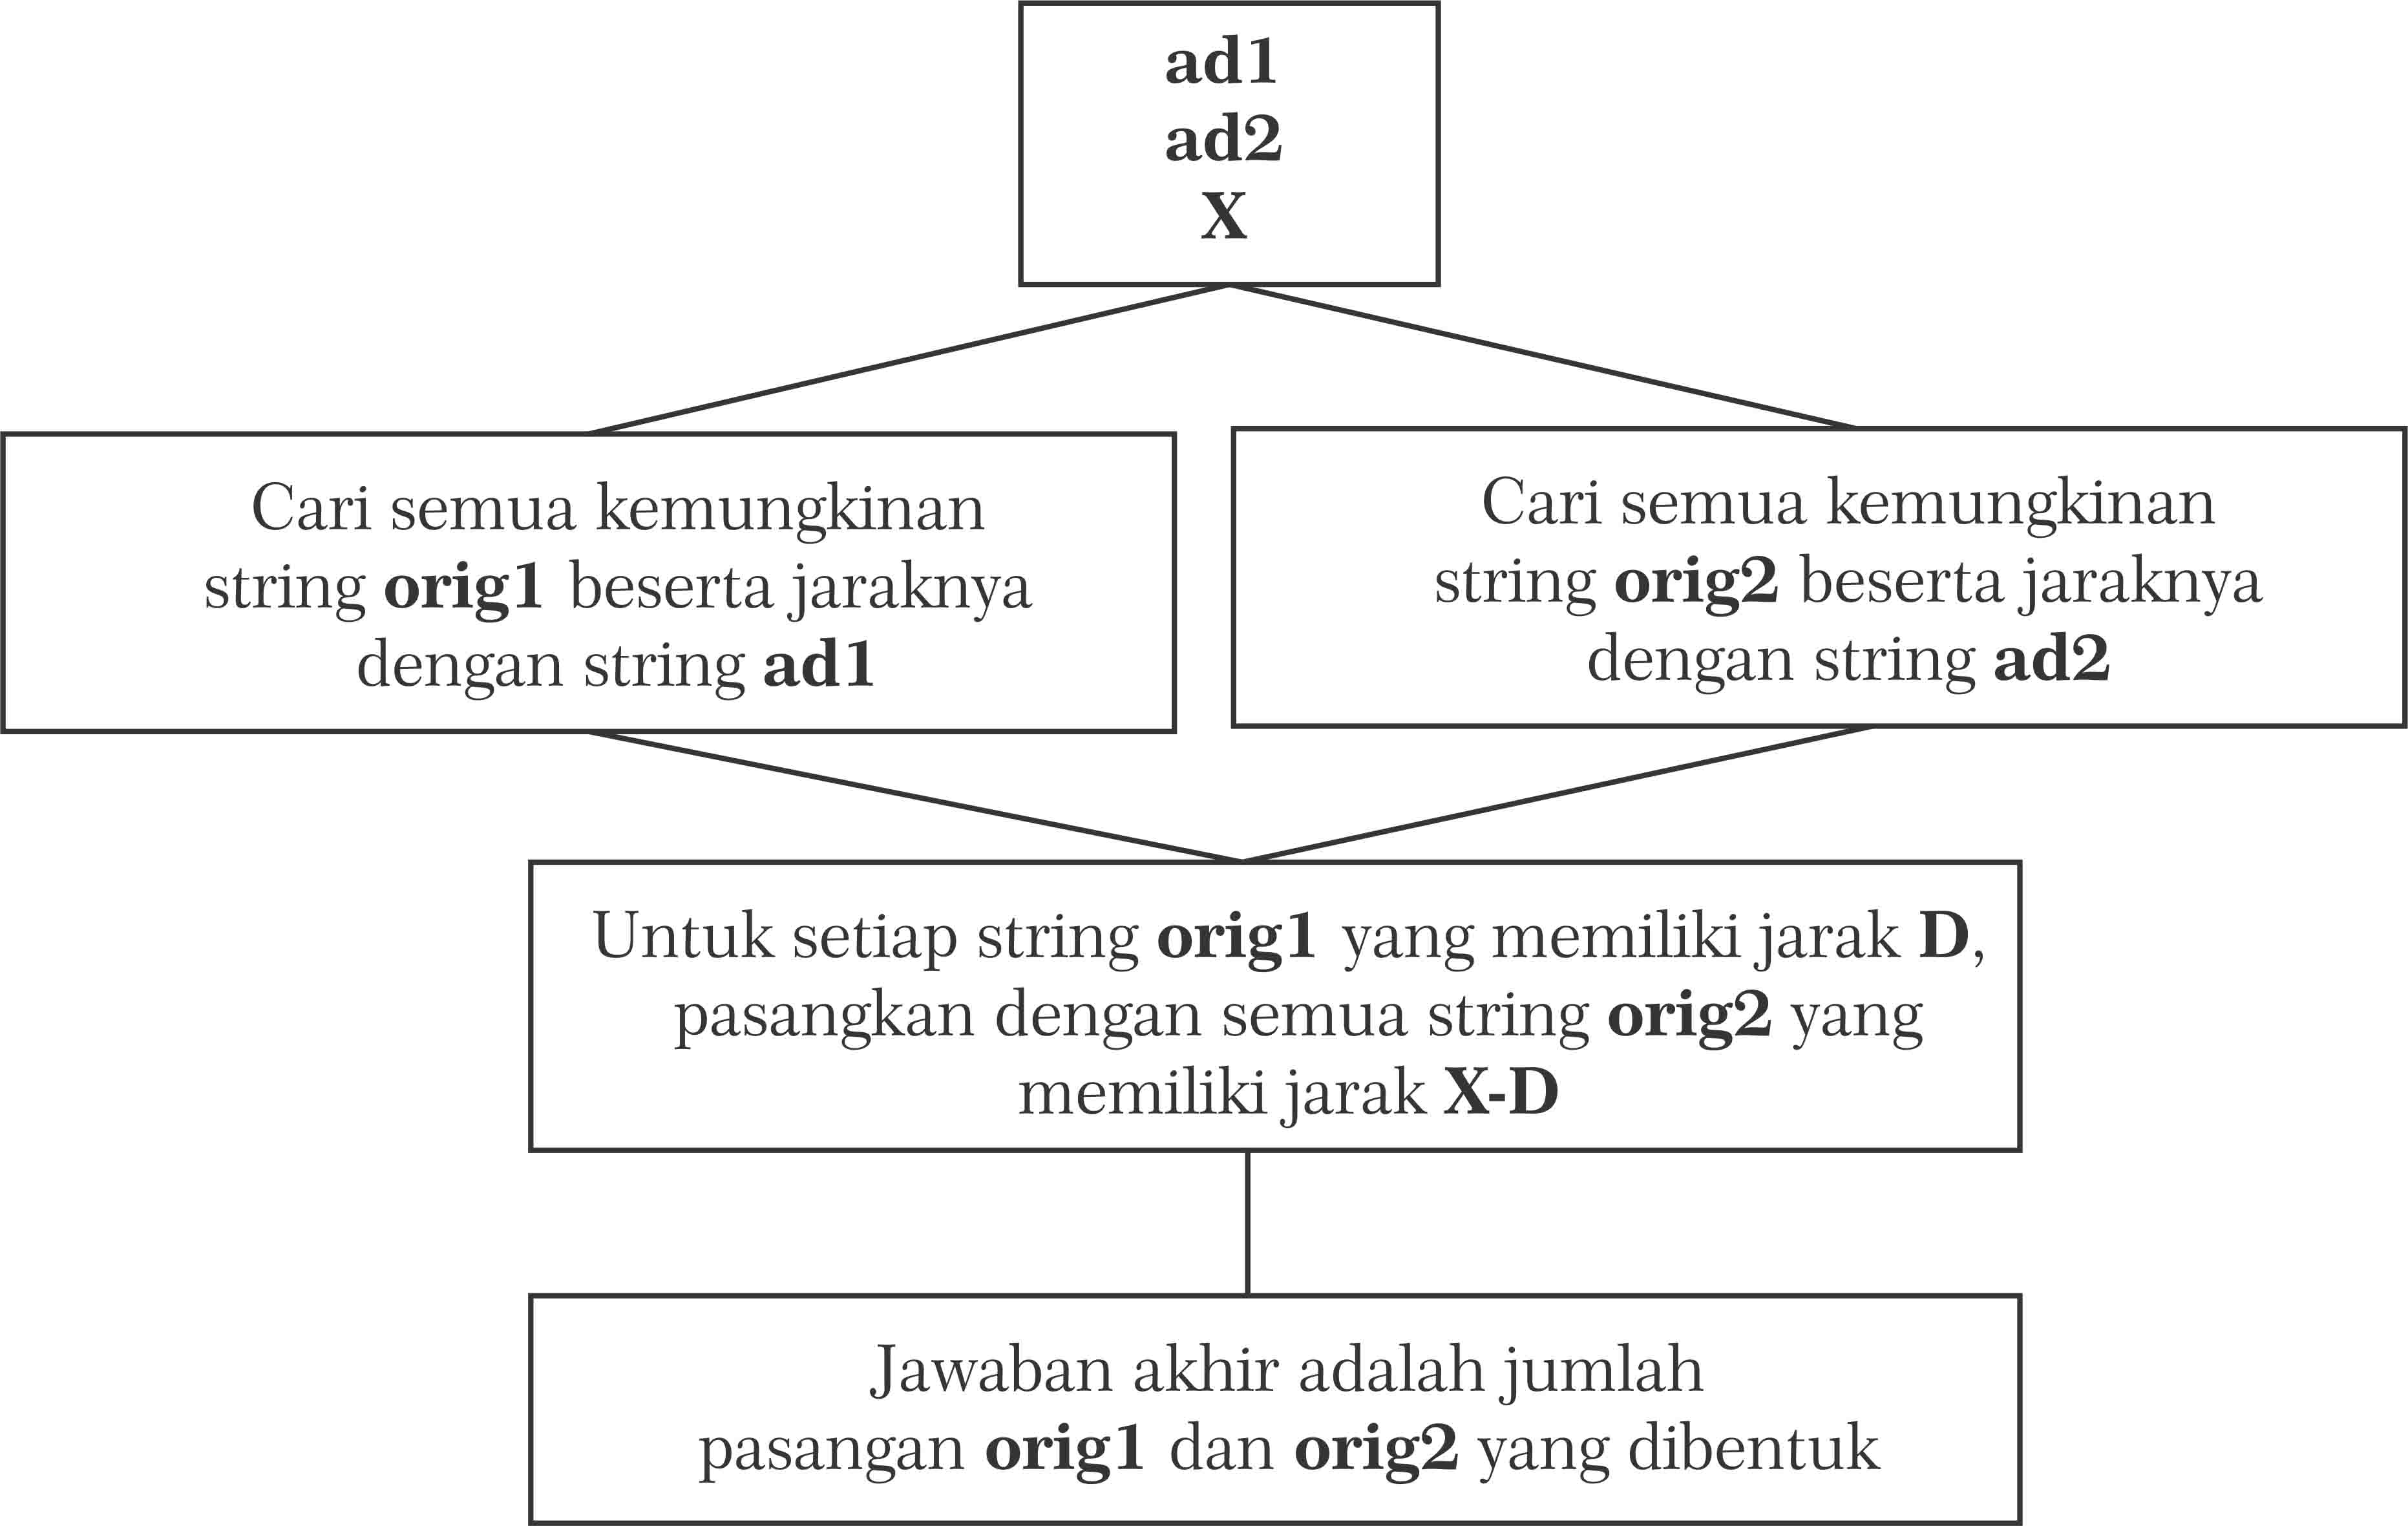
\includegraphics[scale=0.4]{assets/images/jpg/ilustrasi-umum-tanpa-replace.jpg}}
	\caption{Ilustrasi umum penyelesaian permasalahan dengan metode \meetinthemiddle{} tanpa operasi \textit{replace}}
	\label{figure:ilustrasi_umum_penyelesaian_meet_in_the_middle_tanpa_operasi_replace}
\end{figure}

Ketika terdapat operasi \textit{replace}, di mana operasi \textit{replace} adalah operasi di mana salah satu karakter pada \textit{string} $ orig1 $ atau $ orig2 $ diganti dengan karakter sebelumnya atau sesudahnya secara alfabetis, maka perlu dilakukan penyesuaian pada proses perhitungan jawaban. Selain perhitungan kombinasi \textit{string} $ orig1 $ dan \textit{string} $ orig2 $, perlu juga dilakukan perhitungan untuk kombinasi \textit{string} $ orig1 $ dan \textit{string} $ orig2 $ setelah dilakukan satu kali operasi \textit{replace}. Sehingga jawaban akhir dari \problem{} adalah total dari jumlah kemungkinan pasangan \textit{string} $ orig1 $ tanpa operasi \textit{replace} yang memiliki jarak $ D $ terhadap \textit{string} $ ad1 $ dengan \textit{string} $ orig2 $ dengan operasi \textit{replace} yang memiliki jarak $ X - D $ terhadap \textit{string} $ ad2 $ dan jumlah kemungkinan pasangan \textit{string} $ orig1 $ dengan operasi \textit{replace} yang memiliki jarak $ D $ terhadap \textit{string} $ ad1 $ dengan \textit{string} $ orig2 $ tanpa operasi \textit{replace} yang memiliki jarak $ X - D $ terhadap \textit{string} $ ad2 $. Gambar \ref{figure:ilustrasi_umum_penyelesaian_meet_in_the_middle_dengan_operasi_replace} adalah ilustrasi umum penyelesaian \problem{} dengan metode \meetinthemiddle{}.

\begin{figure}
	\centerline{ 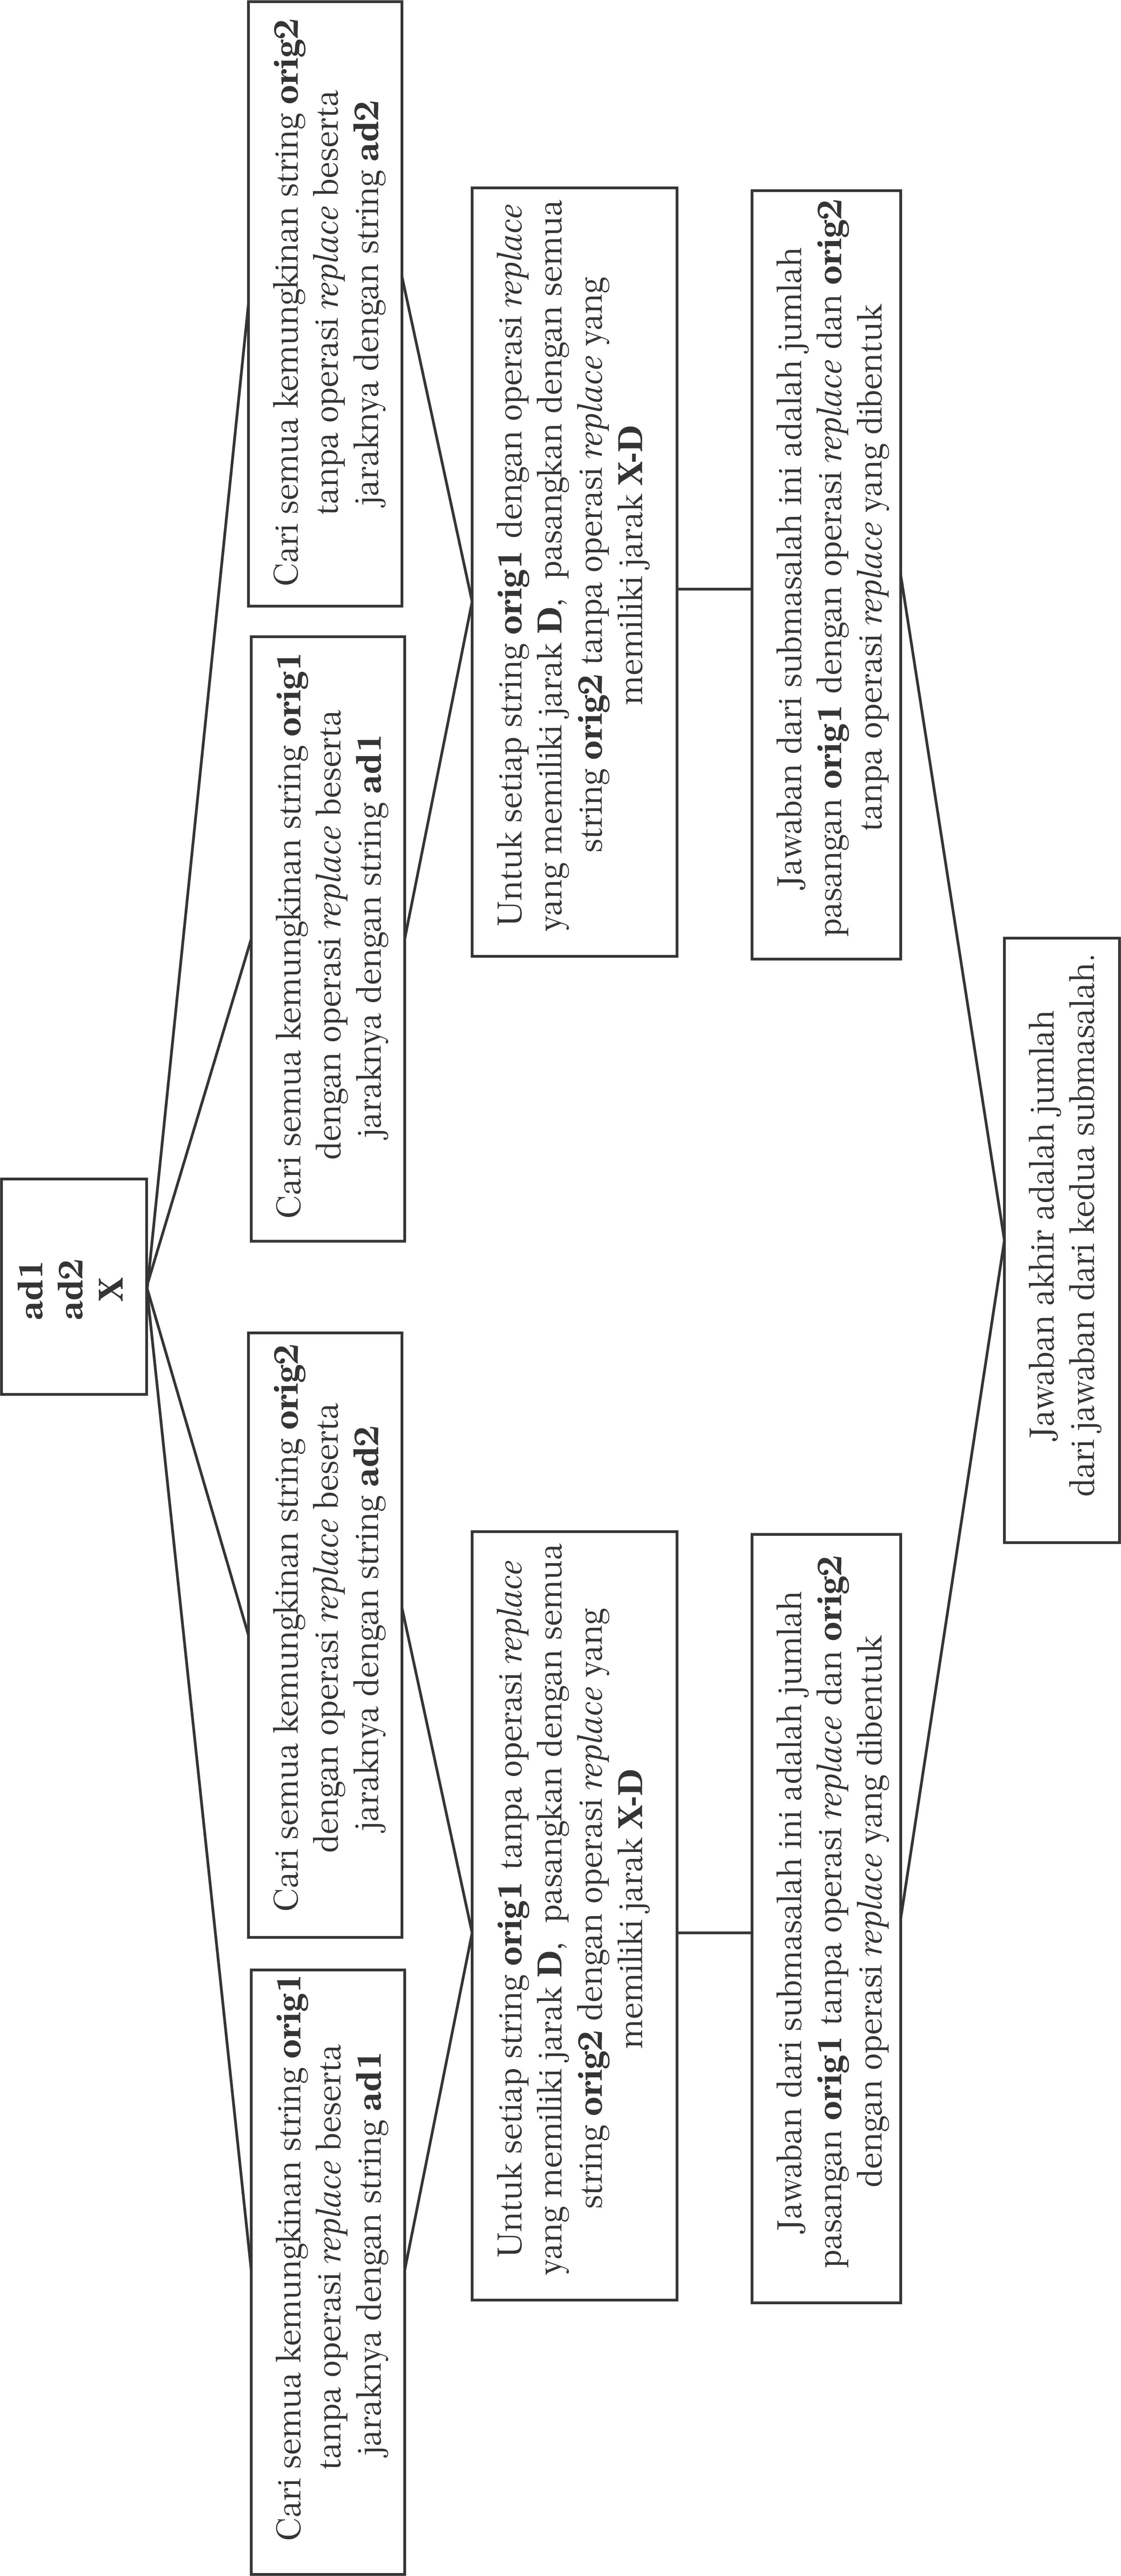
\includegraphics[scale=0.25]{assets/images/jpg/ilustrasi-umum-dengan-replace-rotated.jpg}}
	\caption{Ilustrasi umum penyelesaian permasalahan dengan metode \meetinthemiddle{} dengan operasi \textit{replace}}
	\label{figure:ilustrasi_umum_penyelesaian_meet_in_the_middle_dengan_operasi_replace}
\end{figure}

Sebagai contoh kasus ketika \textit{string} $ orig1=bd $, \textit{string} $ orig2=gj $ dan $ X=5 $. Langkah pertama untuk menyelesaikan kasus ini adalah dengan mencari semua kemungkinan kombinasi \textit{string} $ orig1 $ tanpa operasi \textit{replace} dan semua kemungkinan \textit{string} $ orig2 $ dengan operasi \textit{replace}. Tabel \ref{tab:kombinasi_orig1_bd_tanpa_replace} menunjukkan seluruh kombinasi \textit{string} $ orig1 $ tanpa operasi \textit{replace} beserta jarak masing-masing dengan \textit{string} $ ad1 $ dan Tabel \ref{tab:kombinasi_orig2_gj_dengan_replace} menunjukkan seluruh kombinasi \textit{string} $ orig2 $ dengan operasi \textit{replace} beserta jarak masing-masing dengan \textit{string} $ ad2 $. Berikutnya adalah mencari seluruh pasangan kombinasi \textit{string} $ orig1 $ tanpa operasi \textit{replace} dengan jarak terhadap \textit{string} $ ad1 $ sebesar $ D $ dan kombinasi \textit{string} $ orig2 $ dengan operasi \textit{replace} dengan jarak terhadap \textit{string} $ ad2 $ sebesar $ X-D $ yang hasilnya dapat dilihat pada Tabel \ref{tab:kombinasi_orig1_bd_tanpa_replace_dan_orig2_gj_dengan_replace}. Berikutnya hal yang sama juga dilakukan untuk kombinasi \textit{string} $ orig1 $ dengan operasi \textit{replace} dan \textit{string} $ orig2 $ tanpa operasi \textit{replace}. Tabel \ref{tab:kombinasi_orig1_bd_dengan_replace} menunjukkan seluruh kombinasi \textit{string} $ orig1 $ dengan operasi \textit{replace} beserta jarak masing-masing dengan \textit{string} $ ad1 $ dan Tabel \ref{tab:kombinasi_orig2_gj_tanpa_replace} menunjukkan seluruh kombinasi \textit{string} $ orig2 $ tanpa operasi \textit{replace} beserta jarak masing-masing dengan \textit{string} $ ad2 $. Berikutnya adalah mencari seluruh pasangan kombinasi \textit{string} $ orig1 $ dengan operasi \textit{replace} dengan jarak terhadap \textit{string} $ ad1 $ sebesar $ D $ dan kombinasi \textit{string} $ orig2 $ dengan operasi \textit{replace} tanpa jarak terhadap \textit{string} $ ad2 $ sebesar $ X-D $ yang hasilnya dapat dilihat pada Tabel \ref{tab:kombinasi_orig1_bd_dengan_replace_dan_orig2_gj_tanpa_replace}. Jawaban akhir dari kasus ketika \textit{string} $ orig1=bd $, \textit{string} $ orig2=gj $ dan $ X=5 $ adalah jumlah dari kombinasi pasangan \textit{string} $ orig1 $ dan \textit{string} $ orig2 $ pada Tabel \ref{tab:kombinasi_orig1_bd_tanpa_replace_dan_orig2_gj_dengan_replace} dan Tabel \ref{tab:kombinasi_orig1_bd_dengan_replace_dan_orig2_gj_tanpa_replace}.

\begin{table}
	\centering
	\begin{tabular}{|l|l|l|} \hline
		$ orig1 $ & Jarak dengan $ ad1 $\\ \hline
		$bd$ & $0$ \\ \hline
		$db$ & $4$ \\ \hline
	\end{tabular}
	\caption{Kombinasi \textit{string} $orig1$ dengan nilai \textit{string} $ ad1=bd $ tanpa operasi \textit{replace}}
	\label{tab:kombinasi_orig1_bd_tanpa_replace}
\end{table}

\begin{table}
	\centering
	\begin{tabular}{|l|l|l|} \hline
		$ orig2 $ & Jarak dengan $ ad2 $\\ \hline
		$fj$ & $1$ \\ \hline
		$hj$ & $1$ \\ \hline
		$gi$ & $1$ \\ \hline
		$gk$ & $1$ \\ \hline
		$ig$ & $5$ \\ \hline
		$kg$ & $7$ \\ \hline
		$jf$ & $7$ \\ \hline
		$jh$ & $5$ \\ \hline
	\end{tabular}
	\caption{Kombinasi \textit{string} $orig2$ dengan nilai \textit{string} $ ad2=gj $ dengan operasi \textit{replace}}
	\label{tab:kombinasi_orig2_gj_dengan_replace}
\end{table}

\begin{table}
	\centering
	\begin{tabular}{|l|l|l|l|} \hline
		$ orig1 $ & Jarak dengan $ ad1 $ & $ orig2 $ & Jarak dengan $ ad2 $\\ \hline
		$bd$ & $0$ & $ig$ & $5$\\ \hline
		$bd$ & $0$ & $jh$ & $5$\\ \hline
		$db$ & $4$ & $fj$ & $1$\\ \hline
		$db$ & $4$ & $hj$ & $1$\\ \hline
		$db$ & $4$ & $gi$ & $1$\\ \hline
		$db$ & $4$ & $gk$ & $1$\\ \hline
	\end{tabular}
	\caption{Kombinasi \textit{string} $orig1$ dengan nilai \textit{string} $ ad1=bd $ tanpa operasi \textit{replace} dan  \textit{string} $orig2$ dengan nilai \textit{string} $ ad2=gj $ dengan operasi \textit{replace} dengan $ X=5 $}
	\label{tab:kombinasi_orig1_bd_tanpa_replace_dan_orig2_gj_dengan_replace}
\end{table}

\begin{table}
	\centering
	\begin{tabular}{|l|l|l|} \hline
		$ orig1 $ & Jarak dengan $ ad1 $\\ \hline
		$ad$ & $1$ \\ \hline
		$cd$ & $1$ \\ \hline
		$bc$ & $1$ \\ \hline
		$be$ & $1$ \\ \hline
		$cb$ & $3$ \\ \hline
		$eb$ & $5$ \\ \hline
		$da$ & $5$ \\ \hline
		$dc$ & $3$ \\ \hline
	\end{tabular}
	\caption{Kombinasi \textit{string} $orig1$ dengan nilai \textit{string} $ ad1=bd $ dengan operasi \textit{replace}}
	\label{tab:kombinasi_orig1_bd_dengan_replace}
\end{table}

\begin{table}
	\centering
	\begin{tabular}{|l|l|l|} \hline
		$ orig2 $ & Jarak dengan $ ad2 $\\ \hline
		$gj$ & $0$ \\ \hline
		$jg$ & $6$ \\ \hline
	\end{tabular}
	\caption{Kombinasi \textit{string} $orig2$ dengan nilai \textit{string} $ ad2=gj $ tanpa operasi \textit{replace}}
	\label{tab:kombinasi_orig2_gj_tanpa_replace}
\end{table}

\begin{table}
	\centering
	\begin{tabular}{|l|l|l|l|} \hline
		$ orig1 $ & Jarak dengan $ ad1 $ & $ orig2 $ & Jarak dengan $ ad2 $\\ \hline
		$eb$ & $5$ & $gj$ & $0$\\ \hline
		$da$ & $5$ & $gj$ & $0$\\ \hline
	\end{tabular}
	\caption{Kombinasi \textit{string} $orig1$ dengan nilai \textit{string} $ ad1=bd $ dengan operasi \textit{replace} dan  \textit{string} $orig2$ dengan nilai \textit{string} $ ad2=gj $ tanpa operasi \textit{replace} dengan $ X=5 $}
	\label{tab:kombinasi_orig1_bd_dengan_replace_dan_orig2_gj_tanpa_replace}
\end{table}

Pada deskripsi \problem{} jawaban akhir adalah banyak kemungkinan \textit{string} $ orig1 $ dan $ orig2 $ tanpa perlu menyertakan daftar \textit{string} $ orig1 $ dan $ orig2 $ yang mungkin. Maka dari itu, proses perhitungan jawaban akhir dapat disederhanakan agar algoritma yang dibangun lebih optimal. Seperti yang terlihat pada ilustrasi umum penyelesaian pada Gambar \ref{figure:ilustrasi_umum_penyelesaian_meet_in_the_middle_dengan_operasi_replace_tanpa_kombinasi}, proses pencarian kombinasi \textit{string} $ orig1 $ dan $ orig2 $ dapat diganti dengan hanya menghitung jumlah kemungkinan kombinasi \textit{string} $ orig1 $ dengan atau tanpa operasi \textit{replace} dengan jarak terhadap \textit{string} $ ad1 $ sebesar $ D $ dan jumlah kemungkinan kombinasi \textit{string} $ orig2 $ dengan atau tanpa operasi \textit{replace} dengan jarak terhadap \textit{string} $ ad2 $ sebesar $ D $ dengan $ 0 \le D \le X $.

\begin{figure}
	\centerline{ 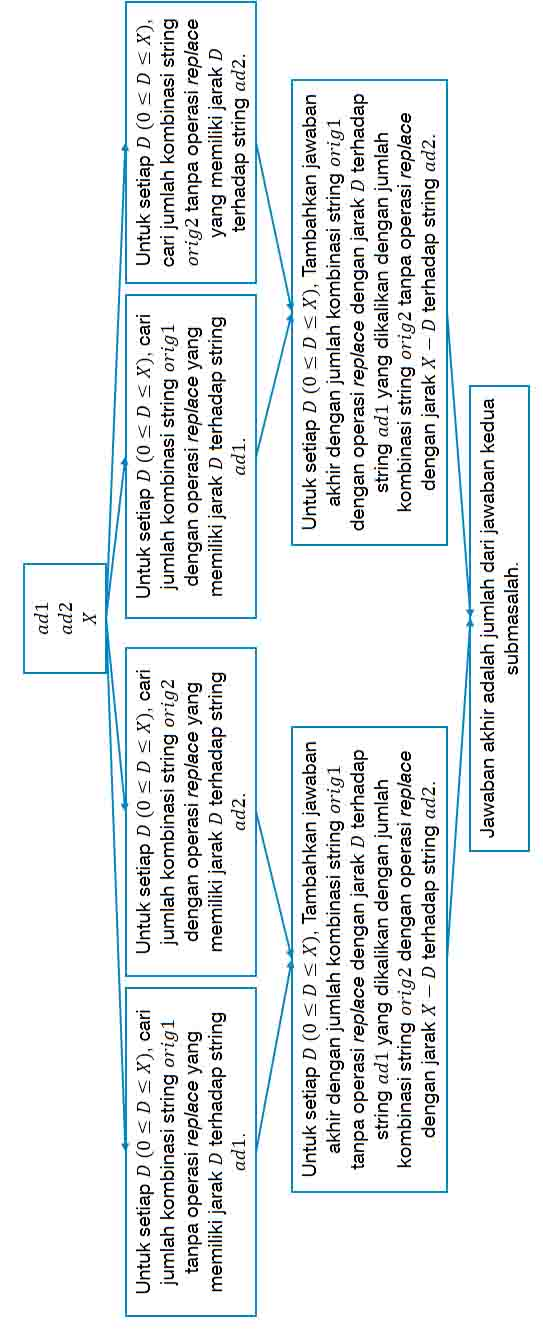
\includegraphics[scale=0.43]{assets/images/jpg/ilustrasi-umum-optimized-fix.jpg}}
	\caption{Ilustrasi umum penyelesaian permasalahan dengan metode \meetinthemiddle{} dengan operasi \textit{replace} tanpa mempedulikan kombinasi \textit{string} yang dihasilkan}
	\label{figure:ilustrasi_umum_penyelesaian_meet_in_the_middle_dengan_operasi_replace_tanpa_kombinasi}
\end{figure}

\subsection{Submasalah Optimal untuk Menghitung Jumlah Kombinasi \textit{String} $ Orig $ dari \textit{String} $ Ad $ Tanpa Operasi \textit{Replace} dengan Jarak $D$}
\label{subsec:submasalah_optimal_untuk_menghitung_jumlah_kombinasi_string_orig_dari_string_ad_tanpa_operasi_replace}
Ilustrasi pada Gambar \ref{figure:ilustrasi_umum_penyelesaian_meet_in_the_middle_dengan_operasi_replace_tanpa_kombinasi} menunjukkan bahwa untuk mendapatkan jawaban akhir dari \problem{} salah satu langkah yang harus dilakukan adalah menghitung jumlah kombinasi \textit{string} $ orig $ dari \textit{string} $ ad $ tanpa operasi \textit{replace} dengan jarak $ D $. Terdapat dua kali perhitungan untuk proses ini yaitu perhitungan untuk mencari jumlah kombinasi \textit{string} $ orig1 $ dan \textit{string} $ orig2 $ tanpa operasi \textit{replace} dengan jarak $ D $.

Perhitungan jumlah kombinasi \textit{string} $ orig $ tanpa operasi \textit{replace} dapat dilakukan dengan memanfaatkan teknik \textit{bitmasking}. Gambar \ref{figure:ilustrasi_perhitungan_kombinasi_orig_tanpa_replace} adalah ilustrasi perhitungan kombinasi \textit{string} $ orig $ dari \textit{string} $ ad $ dengan nilai \textit{string} $ ad=bcd $ dan $ D=4 $ tanpa operasi \textit{replace}. Nilai dari suatu \textit{state} adalah jumlah dari nilai seluruh \textit{state} yang merupakan \textit{child} dari \textit{state} tersebut dengan kasus dasar pada \textit{state} dengan $ mask=0 $, apabila $ jarak=D $ maka \textit{state} tersebut akan bernilai $ 1 $, jika tidak maka akan bernilai $ 0 $.

Namun, seperti yang dapat dilihat pada Gambar \ref{figure:contoh_kasus_tumpang_tindih}, terdapat beberapa kasus di mana pada suatu \textit{state}, \textit{state} dengan nilai tersebut bersifat tumpang tindih dengan suatu \textit{state} lain. Pada Gambar \ref{figure:contoh_kasus_tumpang_tindih}, \textit{state} yang saling tumpang tindih ditandai dengan tulisan berwarna merah. Dengan adanya kasus \textit{state} yang tumpang tindih tersebut dapat dimanfaatkan untuk melakukan optimasi pada algoritma yang dirancang dengan tidak melakukan perhitungan ulang pada \textit{state} yang sudah pernah muncul sebelumnya. Sehingga proses perhitungan yang sebelumnya seperti dengan ilustrasi pada Gambar \ref{figure:ilustrasi_perhitungan_kombinasi_orig_tanpa_replace} dapat disederhanakan menjadi seperti yang terdapat pada Gambar \ref{figure:ilustrasi_perhitungan_kombinasi_orig_tanpa_replace_optimal}. Teknik tersebut dikenal dengan teknik \dynamicprogramming{}.

\begin{figure}
	\centerline{ \includegraphics[scale=0.3]{assets/images/new/jpg/subproblem1-rotated.jpg}}
	\caption{Ilustrasi perhitungan jumlah kombinasi \textit{string} $ orig $ dari \textit{string} $ ad $ tanpa operasi \textit{replace} dengan nilai \textit{string} $ ad = bcd $ dan $ D=4 $}
	\label{figure:ilustrasi_perhitungan_kombinasi_orig_tanpa_replace}
\end{figure}

\begin{figure}
	\centerline{ \includegraphics[scale=0.3]{assets/images/new/jpg/subproblem1-overlapping-rotated.jpg}}
	\caption{Contoh kasus tumpang tindih pada perhitungan kombinasi \textit{string} $ orig $ dari \textit{string} $ ad $ tanpa operasi \textit{replace} dengan nilai \textit{string} $ ad=bcd $ dan $ D=4 $}
	\label{figure:contoh_kasus_tumpang_tindih}
\end{figure}

\begin{figure}
	\centerline{ 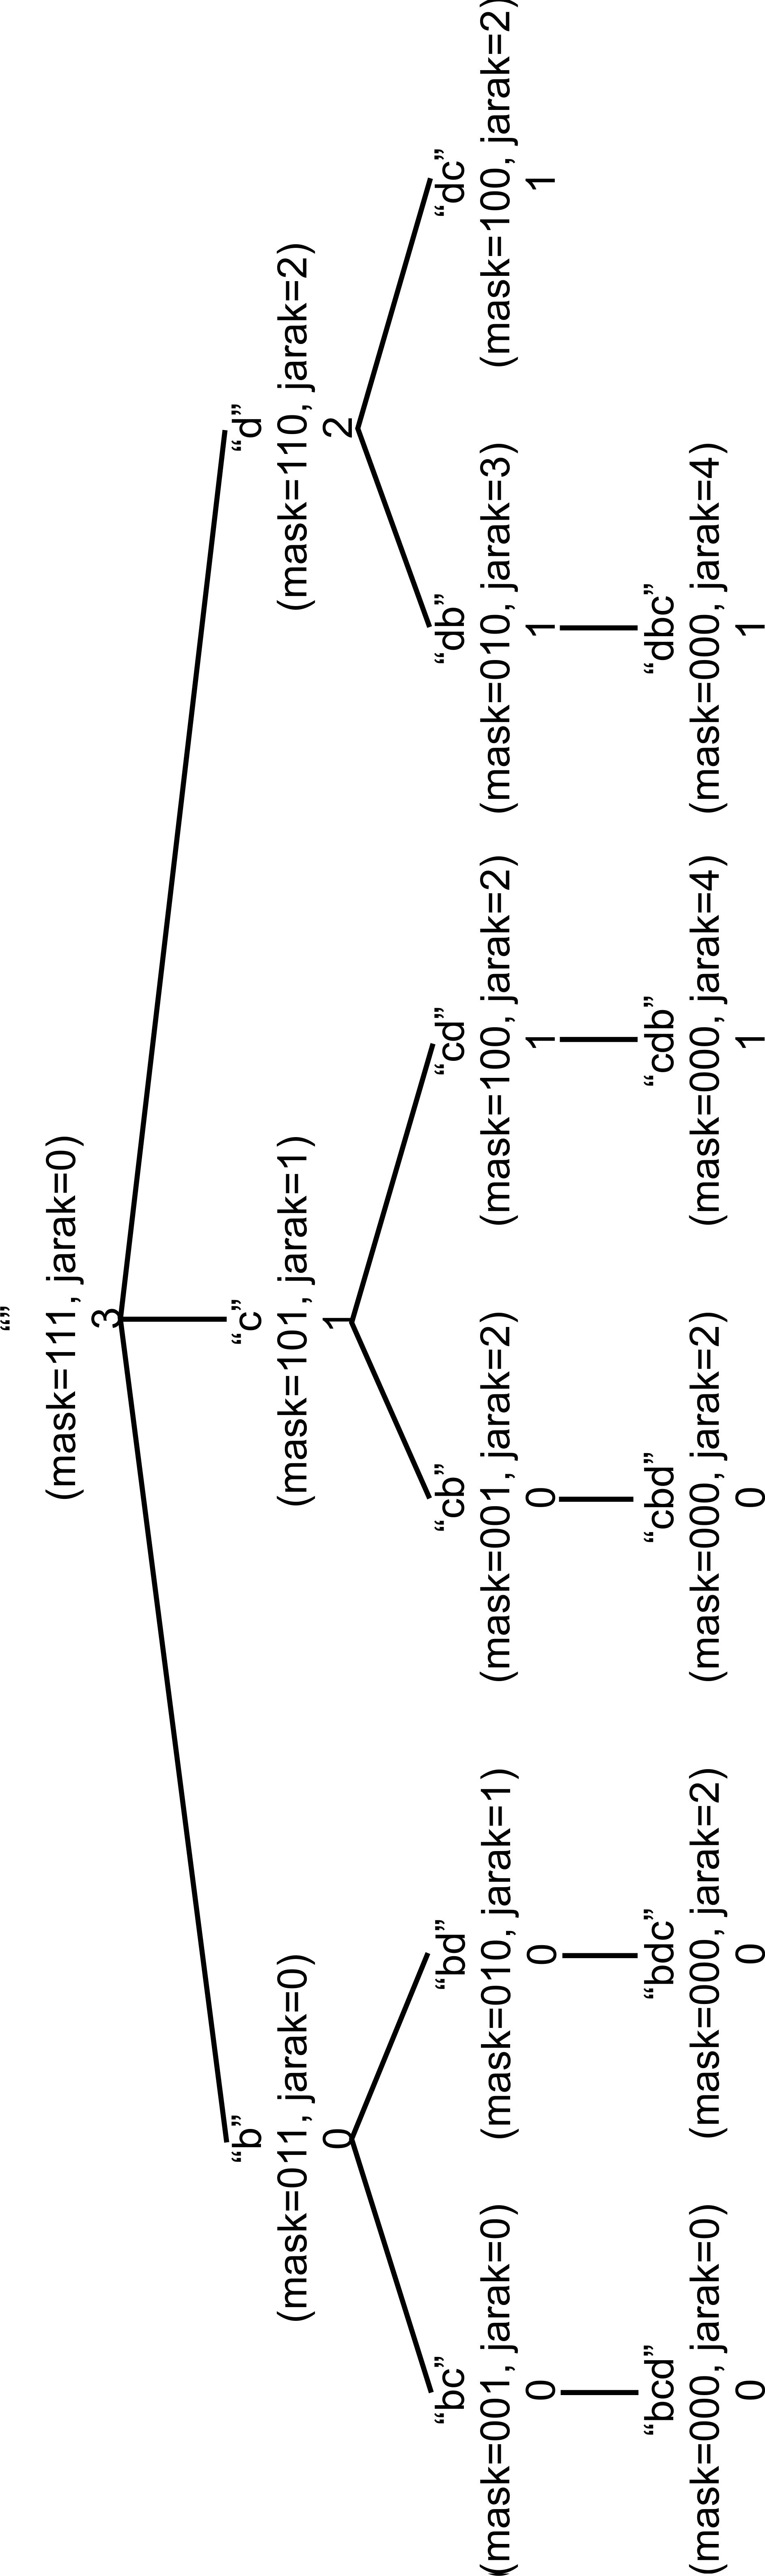
\includegraphics[scale=0.3]{assets/images/new/jpg/subproblem1-optimal-rotated.jpg}}
		\caption{Ilustrasi perhitungan jumlah kombinasi \textit{string} $ orig $ dari \textit{string} $ ad $ tanpa operasi \textit{replace} dengan nilai \textit{string} $ ad = bcd $ dan $ D=4 $ tanpa menghitung kasus yang tumpang tindih}
		\label{figure:ilustrasi_perhitungan_kombinasi_orig_tanpa_replace_optimal}
\end{figure}

\subsection{Submasalah Optimal untuk Menghitung Jumlah Kombinasi \textit{String} $ Orig $ dari \textit{String} $ Ad $ dengan Operasi \textit{Replace} dengan Jarak $D$}
\label{subsec:submasalah_optimal_untuk_menghitung_jumlah_kombinasi_string_orig_dari_string_ad_dengan_operasi_replace}

Ilustrasi pada Gambar \ref{figure:ilustrasi_umum_penyelesaian_meet_in_the_middle_dengan_operasi_replace_tanpa_kombinasi} menunjukkan bahwa untuk mendapatkan jawaban akhir dari \problem{} salah satu langkah yang harus dilakukan adalah menghitung jumlah kombinasi \textit{string} $ orig $ dari \textit{string} $ ad $ dengan operasi \textit{replace} dengan jarak $ D $. Terdapat dua kali perhitungan untuk proses ini yaitu perhitungan untuk mencari jumlah kombinasi \textit{string} $ orig1 $ dan \textit{string} $ orig2 $ tanpa operasi \textit{replace} dengan jarak $ D $.

Cara untuk mendapatkan jawaban dari submasalah ini hampir sama dengan cara mencari jawaban pada submasalah perhitungan jumlah kombinasi \textit{string} $ orig $ dari \textit{string} $ ad $ tanpa operasi \textit{replace}. Gambar \ref{figure:ilustrasi_perhitungan_kombinasi_orig_dengan_replace} merupakan ilustrasi dari penyelesaian submasalah perhitungan jumlah kombinasi \textit{string} $ orig $ dari \textit{string} $ ad $ dengan operasi \textit{replace} dengan nilai $ ad=be $ dan $ D=1 $. Sedikit berbeda dengan penyelesaian submasalah perhitungan jumlah kombinasi \textit{string} $ orig $ dari \textit{string} $ ad $ tanpa operasi \textit{replace}, pada penyelesaian submasalah ini terdapat satu parameter lagi pada setiap \textit{state}, yaitu penanda bahwa pada \textit{state} tersebut sudah pernah melakukan operasi \textit{replace} atau belum.

Sama seperti pada penyelesaian submasalah perhitungan jumlah kombinasi \textit{string} $ orig $ dari \textit{string} $ ad $ tanpa operasi \textit{replace}, pada submasalah perhitungan jumlah kombinasi \textit{string} $ orig $ dari \textit{string} $ ad $ dengan operasi \textit{replace} juga memiliki \textit{state} yang saling tumpang tindih seperti yang terlihat pada Gambar \ref{figure:contoh_kasus_tumpang_tindih_2} sehingga dapat dilakukan optimasi menggunakan teknik \dynamicprogramming{} untuk meningkatkan efisiensi algoritma yang dibangun. Pada Gambar \ref{figure:submasalah_1_pada_submasalah_2} dapat dilihat bahwa terdapat beberapa \textit{state} yang ternyata memiliki kondisi yang mampu diselesaikan dengan metode yang sama dengan metode penyelesaian submasalah perhitungan jumlah kombinasi \textit{string} $ orig $ dari \textit{string} $ ad $ tanpa operasi \textit{replace}. Sehingga penyelesaian submasalah perhitungan jumlah kombinasi \textit{string} $ orig $ dari \textit{string} $ ad $ dengan operasi \textit{replace} dapat disederhanakan dengan memanfaatkan penyelesaian submasalah perhitungan jumlah kombinasi \textit{string} $ orig $ dari \textit{string} $ ad $ tanpa operasi \textit{replace}.

\begin{figure}
	\centerline{ \includegraphics[scale=0.25]{assets/images/new/jpg/subproblem2-rotated.jpg}}
	\caption{Ilustrasi perhitungan jumlah kombinasi \textit{string} $ orig $ dari \textit{string} $ ad $ dengan operasi \textit{replace} dengan nilai \textit{string} $ ad = be $ dan $ D=1 $}
	\label{figure:ilustrasi_perhitungan_kombinasi_orig_dengan_replace}
\end{figure}

\begin{figure}
	\centerline{ 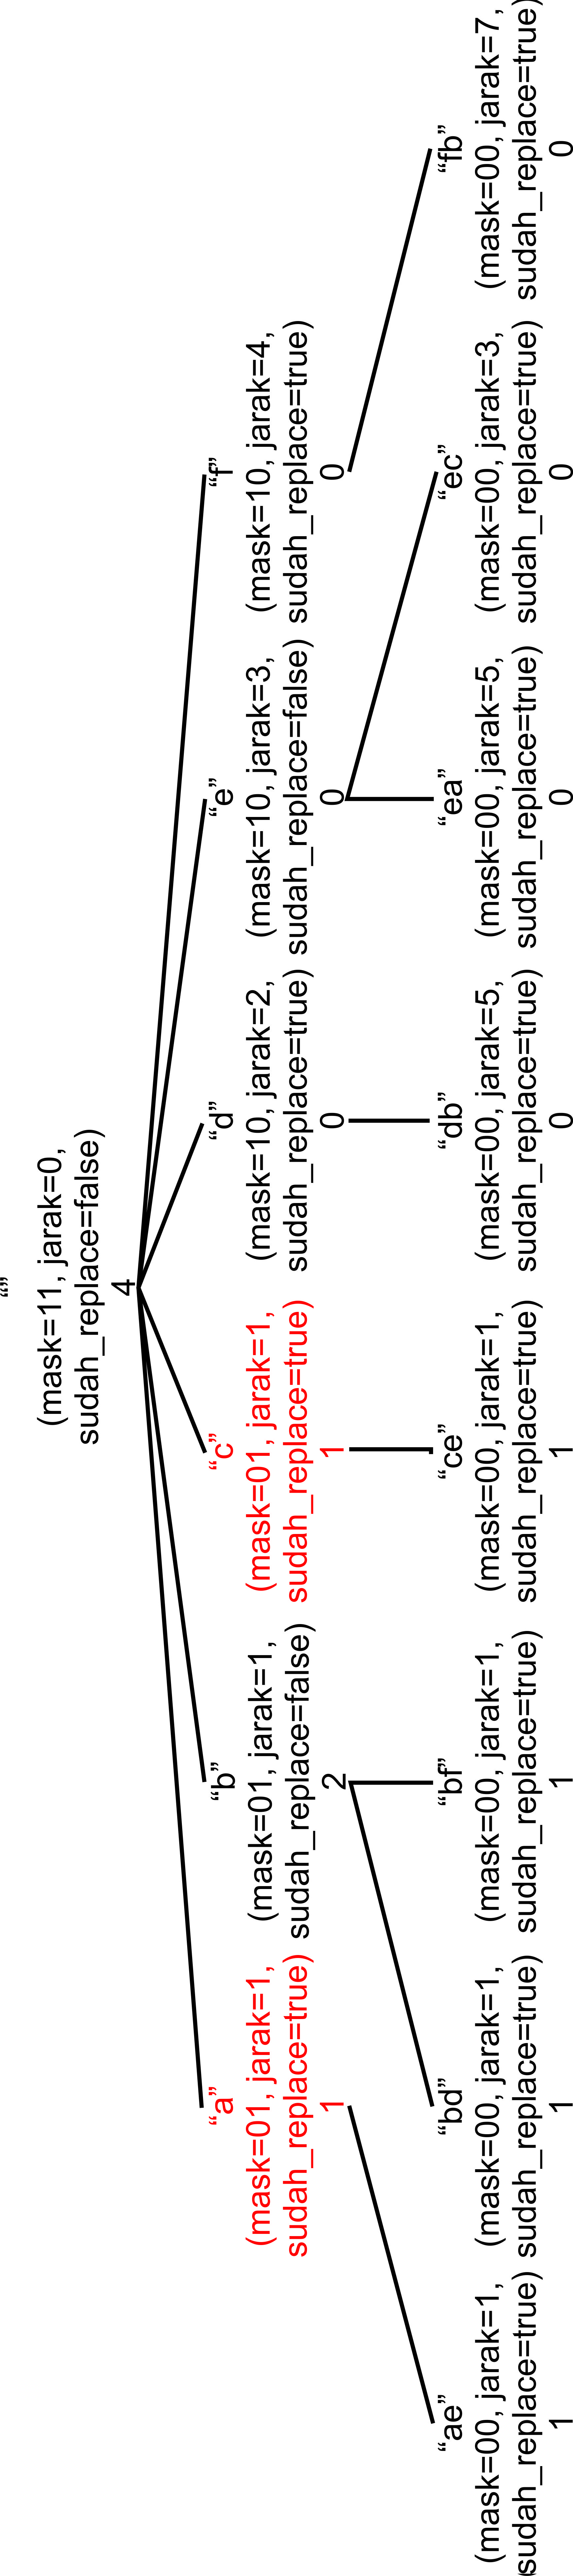
\includegraphics[scale=0.25]{assets/images/new/jpg/subproblem2-overlapping-rotated.jpg}}
	\caption{Contoh kasus tumpang tindih pada perhitungan kombinasi \textit{string} $ orig $ dari \textit{string} $ ad $ dengan operasi \textit{replace} dengan nilai \textit{string} $ ad=be $ dan $ D=1 $}
	\label{figure:contoh_kasus_tumpang_tindih_2}
\end{figure}

\begin{figure}
	\centerline{ 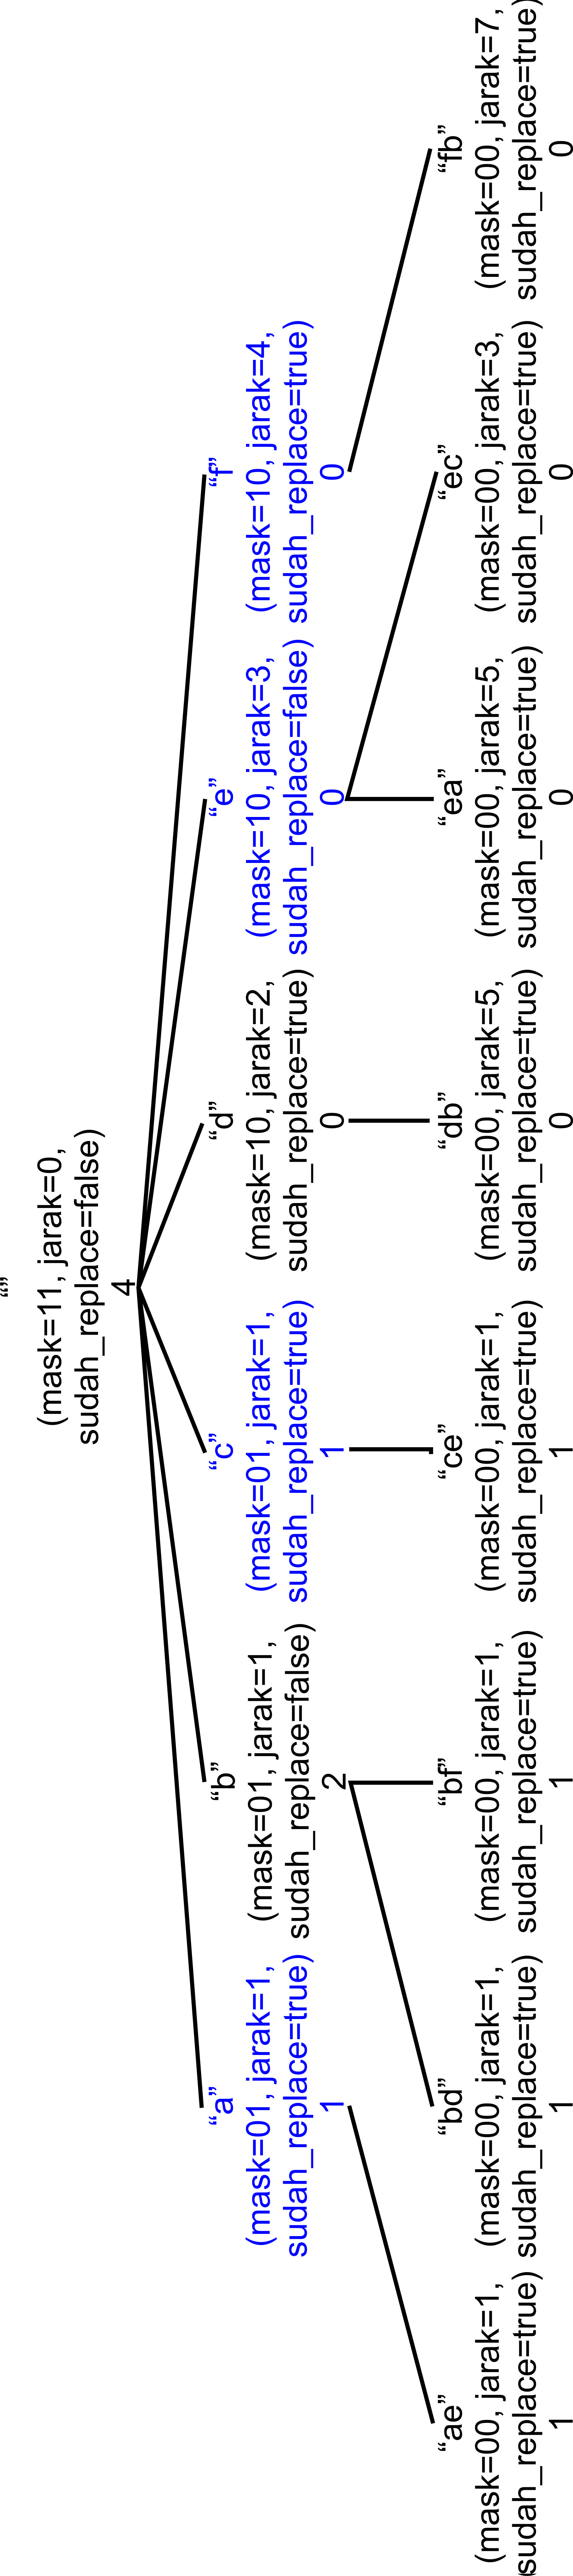
\includegraphics[scale=0.25]{assets/images/new/jpg/subproblem2-tipe1-rotated.jpg}}
	\caption{Submasalah perhitungan jumlah kombinasi \textit{string} $ orig $ terhadap \textit{string} $ ad $ tanpa operasi \textit{replace} pada submasalah perhitungan jumlah kombinasi \textit{string} $ orig $ terhadap \textit{string} $ ad $ dengan operasi \textit{replace}}
	\label{figure:submasalah_1_pada_submasalah_2}
\end{figure}


\section{Pemodelan Relasi Rekurens}
\label{sec:pemodelan_relasi_rekurens}
    
\begin{equation}
answer = \parbox[t]{0.9\textwidth}{ $\sum_{dist=0}^{dist=min_{(X, 250)}}((F_{(S_{0}, 2^{|S_{0}|}, bound - dist)} * G_{(S_{1}, 2^{|S_{1}|}, bound - X + dist)}) + (G_{(S_{0}, 2^{|S_{0}|}, bound -dist)} * F_{(S_{1},2^{|S_{1}|},bound-X+dist)}))$}
\label{equation:main_answer}
\end{equation}    
    
Pada subbab ini akan dijelaskan tentang relasi rekurens berdasarkan analisis pada subbab \ref{sec: analisa_submasalah_optimal}. Pada subbagian \ref{subsec:membagi_permasalahan_menjadi_dua_submasalah_yang_independent}, dijelaskan bahwa permasalahan dapat dipecah menjadi dua submasalah yang dapat diselesaikan tanpa bergantung satu sama lain dengan memecah permasalahan berdasarkan masing-masing \textit{string} $ad$. Karena terdapat sebuah operasi \textit{replace} yang dilakukan, maka untuk menyelesaikan masing-masing submasalah harus dilakukan dua jenis perhitungan, yaitu operasi perhitungan jumlah kemungkinan \textit{string} $orig$ tanpa operasi \textit{replace} dan operasi perhitungan jumlah kemungkinan \textit{string} $orig$ dengan operasi \textit{replace}. Kedua operasi tersebut didefinisikan dalam bentuk fungsi sebagai berikut:
\begin{enumerate}
	\item $F_{(S, mask, dist)}$, yaitu fungsi untuk menghitung jumlah kemungkinan \textit{string} awal dari \textit{string} $ S $ tanpa operasi \textit{replace} di mana $S$ adalah \textit{string} awal yang akan dihitung, $mask$ adalah nilai \textit{bitmask} dan $dist$ adalah jarak \textit{string} awal dengan \textit{string} yang dibentuk pada \textit{state} tersebut.
	\label{itm: fungsi_f}
	\item $G_{(S, mask, dist)}$, yaitu fungsi untuk menghitung jumlah kemungkinan \textit{string} awal dari \textit{string} $ S $ dengan sekali operasi \textit{replace} di mana $S$ adalah \textit{string} awal yang akan dihitung, $mask$ adalah nilai \textit{bitmask} dan $dist$ adalah jarak \textit{string} awal dengan \textit{string} yang dibentuk pada \textit{state} tersebut.
	\label{itm: fungsi_g} 
\end{enumerate}

Jawaban \problem{} dapat dihitung dengan memanfaatkan kedua fungsi di atas. Persamaan \ref{equation:main_answer} merupakan persamaan untuk menghitung jawaban utama dari \problem{} di mana $S_{0}$ adalah \textit{string} $ad1$, $S_{1}$ adalah \textit{string} $ad2$, $X$ adalah jumlah jarak($ad1$, $orig1$) dengan jarak($ad2$, $orig2$) dan $bound=min(250, X)$ dengan Tabel \ref{tab:daftar_notasi_main_answer} adalah daftar notasi yang digunakan pada persamaan tersebut. Nilai $ bound = min(250, X) $ memiliki arti batas atas variabel $ bound $ adalah $ 250 $ karena panjang \textit{string} masukan dijamin tidak lebih dari $ 10 $ karakter yang artinya jarak antar dua \textit{string} pada \problem{} tidak mungkin melebihi angka $ 250 $. Sehingga apabila nilai masukan $ X>250 $ dapat diasumsikan bahwa hal tersebut tidak mungkin. 

\begin{table}[H]
	\centering
	\begin{tabular} {|p{3cm}|p{5cm}|} \hline
		Notasi & Deskripsi\\ \hline
		$ dist $ & Nilai jarak yang diiterasi dari 0 hingga $ min(X, 250) $\\ \hline
		$ X $ & Masukan yang merepresentasikan jumlah jarak \textit{string} $ orig1 $ dengan \textit{string} $ ad1 $ dan jarak \textit{string} $ orig2 $ dengan \textit{string} $ ad2 $ \\ \hline
		$ S_{0} $ & \textit{String} masukan yang merepresentasikan $ ad1 $\\ \hline
		$ S_{1} $ & \textit{String} masukan yang merepresentasikan $ ad2 $\\ \hline
		$ |S_{0}| $ & Panjang \textit{string} $ ad1 $\\ \hline
		$ |S_{1}| $ & Panjang \textit{string} $ ad2 $\\ \hline
		$ bound $ & Nilai batas jarak maksimal yang bernilai $ min(X, 250) $\\ \hline
	\end{tabular}\caption{Daftar notasi persamaan \ref{equation:main_answer}}
	\label{tab:daftar_notasi_main_answer}
\end{table}

\subsection{Pemodelan Relasi Rekurens Submasalah Optimal untuk Menghitung Jumlah Kemungkinan \textit{String} Awal Tanpa Operasi \textit{Replace} dengan Jarak $X-dist$}
\label{subsec:pemodelan_relasi_rekurens_submasalah_optimal_untuk_menghitung_jumlah_kemungkinan_string_awal_tanpa_operasi_replace}

\begin{table}
	\centering
	\begin{tabular} {|p{3cm}|p{5cm}|} \hline
		Notasi & Deskripsi\\ \hline
		$ S $ & \textit{String} yang akan dicari kemungkinan \textit{string} awalnya.\\ \hline
		$ mask $ & Sebuah bilangan bulat yang bertugas sebagai \textit{bitmask} yang merepresentasikan kondisi karakter mana saja yang sudah diambil pada kondisi (\textit{state}) tersebut.\\ \hline
		$ dist $ & Jarak \textit{string} yang sudah terbentuk pada kondisi tersebut dengan \textit{string} $ S $ dari $ bound $ atau secara matematis dapat dituliskan dengan $ bound - distance(currentString, S) $.\\ \hline
		$ bound $ & Nilai batas jarak maksimal yang bernilai $ min(X, 250) $\\ \hline
		$ idx $ & Index karakter pada \textit{string} $ S $ yang akan diambil atau digunakan.\\ \hline
		$ NSB_{(mask)} $ & Mengembalikan jumlah angka 1 pada $ mask $ apabila direpresentasikan dalam basis biner\\ \hline
		$ set\_bit_{(mask)} $ & Himpunan index bilangan bernilai satu dari $ mask $ apabila direpresentasikan dalam basis biner.\\ \hline
		$ is\_on_{(mask, idx)} $ & Mengembalikan nilai $ true $ apabila bilangan pada index $ idx $ pada $ mask $ bernilai $ 1 $ apabila direpresentasikan dalam basis biner.\\ \hline
	\end{tabular}\caption{Daftar notasi persamaan \ref{equation:rekurens_f}, \ref{equation:rekurens_f1} dan \ref{equation:rekurens_duplicate_rule1}}
	\label{tab:daftar_notasi_f}
\end{table}

\begin{equation}
F_{(S, mask, dist)} = \begin{cases}
0, & \parbox[t]{.3\textwidth}{if $dist > bound$ or ($mask=0$ and $dist \neq bound$)}, \\
1, & \parbox[t]{.3\textwidth}{if $mask=0$ and $dist=bound$}, \\
\sum_{i=0}^{i=NSB_{(mask)}} \\F1_{(S, mask,
	set\_bit(mask)_{i}, dist)} ,& \text{otherwise}
\end{cases}
\label{equation:rekurens_f}
\end{equation}



\begin{equation}
F1_{(S, mask, idx, dist)} = 
\begin{cases}
F_{(S, mask - 2^{idx}, dist +}\\_{|S_{idx} - S_{curIdx}|)}
, & \parbox[t]{.3\textwidth}{idx = |S| - 1 or $duplicate\_rule1_{(S, mask, idx)} = True$}\\
0, & \text{otherwise}
\end{cases}
\label{equation:rekurens_f1}
\end{equation}


\begin{equation}
duplicate\_rule1_{(S, mask, idx)} = 
\begin{cases}
True, & \parbox[t]{.3\textwidth}{if $idx < |S| -1$ and ($S_{idx} \neq S_{idx + 1}$  \text{or} (($S_{idx} = S_{idx + 1}$)  \text{and} ($is\_on_{(mask, idx + 1)} =  False$))}\\
False, & \text{otherwise}
\label{equation:rekurens_duplicate_rule1}
\end{cases}
\end{equation}

\begin{equation*}
	is\_on_{(mask, idx)} = 
	\begin{cases}
		True, & \parbox[t]{.3\textwidth}{($mask$ \& $2^{idx}) = 1$}\\
		False, & \text{otherwise}
	\end{cases}
\end{equation*}

Pada bagian ini akan dijelaskan beberapa persamaan rekurens dengan daftar notasi seperti yang terdapat pada Tabel \ref{tab:daftar_notasi_f}. Pada persamaan \ref{equation:main_answer} terdapat fungsi $F_{(S, mask, dist)}$ yang merupakan fungsi untuk menghitung jumlah kemungkinan \textit{string} $orig$ dari \textit{string} $S$ tanpa operasi \textit{replace} dengan jarak $X-dist$. Nilai dari fungsi $F_{(S, mask, dist)}$ adalah hasil penjumlahan seluruh \textit{state} yang berhubungan, yaitu \textit{state} $F_{(S, mask - 2^{idx}, dist +|S_{idx} - S_{curIdx}|)}$ di mana $curIdx$ adalah jumlah \textit{string} yang sudah dipilih pada \textit{state} tersebut yang direpresentasikan dengan jumlah bit tidak menyala pada $mask$. Tidak semua \textit{state} $F_{(S, mask - 2^{idx}, dist +|S_{idx} - S_{curIdx}|)}$ dijumlahkan untuk mendapatkan nilai dari fungsi $F_{(S, mask, dist)}$. Hanya \textit{state} yang valid yang nilainya dijumlahkan untuk membentuk nilai dari fungsi $F_{(S, mask, dist)}$. Persamaan \ref{equation:rekurens_f1} adalah persamaan rekurens untuk menentukan apakah \textit{state} $F_{(S, mask - 2^{idx}, dist +|S_{idx} - S_{curIdx}|)}$ merupakan \textit{state} yang valid dari sebuah \textit{state} $F_{(S, mask, dist)}$. Persamaan \ref{equation:rekurens_f} adalah relasi rekurens dari submasalah perhitungan jumlah kemungkinan \textit{string} $orig$ dari \textit{string} $S$ tanpa operasi \textit{replace} dengan jarak $X-dist$.

Fungsi $ duplicate\_rule1_{(S, mask, idx)} $ adalah fungsi yang mencegah terjadinya perhitungan kombinasi \textit{string} yang sama secara berulang. Contohnya pada kasus \textit{string} $ S=bcc $. Pada dasarnya, fungsi $ F $ akan melakukan perhitungan seluruh kombinasi \textit{string} $ S $ yang mungkin sehingga hasil dari \textit{string} $ S $ yang memiliki panjang $ 3 $ karakter adalah $ 6 $. Berikut adalah \textit{string} yang merupakan kombinasi dari \textit{string} $ S $ yang memiliki panjang 3 karakter:
\begin{enumerate}
	\item $ S_{0}S_{1}S_{2} $
	\item $ S_{0}S_{2}S_{1} $
	\item $ S_{1}S_{0}S_{2} $
	\item $ S_{1}S_{2}S_{0} $
	\item $ S_{2}S_{0}S_{1} $
	\item $ S_{2}S_{1}S_{0} $
\end{enumerate}

Sehingga apabila \textit{string} $ S=bcc $, maka kombinasi \textit{string} yang terbentuk adalah sebagai berikut:
\begin{enumerate}
	\item $ bcc $
	\item $ bcc $
	\item $ cbc $
	\item $ ccb $
	\item $ cbc $
	\item $ ccb $
\end{enumerate}

Terdapat beberapa \textit{string} yang bersifat duplikat sehingga tidak dapat dikatakan sebagai \textit{string} yang berbeda. Sehingga banyak kombinasi \textit{string} berbeda dari $ S=bcc $ adalah $ 3 $ dengan rincian sebagai berikut:
\begin{enumerate}
	\item $ bcc $
	\item $ cbc $
	\item $ ccb $
\end{enumerate}

Konsep dasar dari fungsi $ duplicate\_rule1_{(S, mask, idx)} $ adalah dengan menerapkan aturan hanya boleh memilih karakter $ S_{idx} $ apabila $ S_{idx} = S_{idx+1} $ dan karakter tersebut telah dipilih sebelumnya, yang secara matematis didefinisikan dengan $ mask \& 2^{idx+1} = 0$.

Untuk penjelasan fungsi $ F_{(S, mask, dist)} $ yang lebih jelas, akan disimulasikan contoh pemanggilan fungsi $ F_{(bcc, 7, 3)} $ pada kasus $ S=bcc $ dan $ X=5 $. Berikut adalah penjelasan rinci dari parameter fungsi yang dipanggil:
\begin{enumerate}
	\item Parameter pertama yang bernilai $ bcc $ memiliki arti \textit{string} masukan yang akan dicari jumlah kombinasi \textit{string} awalnya tanpa operasi \textit{replace} adalah $ S=bcc $.
	\item Parameter kedua yang bernilai $ 7 $ merepresentasikan bahwa pada \textit{state} tersebut nilai $ mask = 7 $ atau apabila direpresentasikan dalam basis biner bernilai $ mask = 111_{(2)} $ yang artinya pada \textit{state} tersebut belum ada karakter pada $ S $ yang dipilih untuk melengkapi kombinasi \textit{string} yang akan dicari.
	\item parameter ketiga yang bernilai $ 3 $ merepresentasikan bahwa pada \textit{state} tersebut nilai $ dist = 3 $ yang artinya pada \textit{state} tersebut membutuhkan jarak sebesar $ bound - 3$ untuk mencapai kondisi valid sebuah kombinasi \textit{string} awal di mana $ bound=5 $.
\end{enumerate}

Karena himpunan $ set\_bit_{(7)} = \{0, 1, 2\} $, maka hasil dari pemanggilan fungsi $ F_{(bcc, 7, 3)} $ adalah hasil dari penjumlahan hasil fungsi-fungsi yang akan dipanggil pada fungsi tersebut. Berikut adalah fungsi-fungsi yang dipanggil pada pemanggilan fungsi $ F_{(bcc, 7, 3)} $:
\begin{enumerate}
	\item $ F1_{(bcc, 7, 0, 3)} $ yang akan memanggil fungsi $ F_{(bcc, 6, 3)} $ karena memenuhi syarat $ duplicate\_rule1_{(bcc, 7, 0)} = True$.
	\item $ F1_{(bcc, 7, 1, 3)} $ yang akan mengembalikan nilai $ 0 $ karena nilai $ idx \neq |S| - 1 $ dan nilai $ duplicate\_rule1_{(bcc, 7, 1)} \neq True$ bukan merupakan kondisi yang memenuhi syarat terpanggilnya fungsi $ F_{(bcc, 5, 4)} $.
	\item $ F1_{(bcc, 7, 2, 3)} $ yang akan memanggil fungsi $ F_{(bcc, 3, 4)} $ karena memenuhi syarat $ idx = |S| - 1 $ di mana $ |S| = 3 $ sehingga $ |S|-1 = 2 $ dan $ idx=2 $.
\end{enumerate}

Proses dilanjutkan secara rekursif, yaitu dengan pemanggilan fungsi $ F_{(bcc, 6, 3)} $. Karena himpunan $ set\_bit_{(6)} = \{1, 2\} $, maka hasil dari pemanggilan fungsi $ F_{(bcc, 6, 3)} $ adalah hasil dari penjumlahan hasil fungsi-fungsi yang akan dipanggil pada fungsi tersebut. Berikut adalah fungsi-fungsi yang dipanggil pada pemanggilan fungsi $ F_{(bcc, 6, 3)} $:
\begin{enumerate}
	\item $ F1_{(bcc, 6, 1, 3)} $ yang akan mengembalikan nilai $ 0 $ karena nilai $ idx \neq |S| - 1 $ dan nilai $ duplicate\_rule1_{(bcc, 6, 0)} \neq True$ bukan merupakan kondisi yang memenuhi syarat terpanggilnya fungsi $ F_{(bcc, 4, 3)} $.
	\item $ F1_{(bcc, 6, 2, 3)} $ yang akan memanggil fungsi $ F_{(bcc, 2, 3)} $ karena memenuhi syarat $ idx = |S| - 1 $ di mana $ |S| = 3 $ sehingga $ |S|-1 = 2 $ dan $ idx=2 $.
\end{enumerate}

Proses berikutnya adalah pemanggilan fungsi $ F_{(bcc, 2, 3)} $. Karena himpunan $ set\_bit_{(2)} = \{1\} $, maka nilai dari fungsi $ F_{(bcc, 2, 3)} $ sama dengan nilai dari satu-satunya fungsi yang dipanggil pada fungsi tersebut, yaitu $ F1_{(bcc, 2, 1, 3)} $. Fungsi $ F1_{(bcc, 2, 1, 3)} $ akan memanggil fungsi $ F_{(bcc, 0, 3)} $ karena memenuhi kondisi nilai $ duplicate\_rule1_{(bcc, 2, 1)} = True$. Fungsi $ F_{(bcc, 0, 3)} $ sendiri akan mengembalikan nilai $ 0 $ karena kondisi ketika $ mask = 0 $ adalah kondisi dasar (\textit{base case}) dan $ dist \neq bound$ di mana $ dist = 3$ dan $ bound=5 $. Sehingga nilai dari fungsi $ F_{(bcc, 2, 3)} =0$, fungsi $ F_{(bcc, 6, 3)} =0$ dan nilai dari fungsi $ F_{(bcc, 7, 3)} = 0$.

Berikutnya adalah perhitungan fungsi $ F_{(bcc, 3, 4)} $.  Karena himpunan $ set\_bit_{(3)} = \{0, 1\} $, maka hasil dari pemanggilan fungsi $ F_{(bcc, 3, 4)} $ adalah hasil dari penjumlahan hasil fungsi-fungsi yang akan dipanggil pada fungsi tersebut. Berikut adalah fungsi-fungsi yang dipanggil pada pemanggilan fungsi $ F_{(bcc, 3, 4)} $:
\begin{enumerate}
	\item $ F1_{(bcc, 3, 0, 4)} $ yang akan memanggil fungsi $ F_{(bcc, 2, 5)} $ karena memenuhi syarat $ duplicate\_rule1_{(bcc, 3, 0)} = True$.
	\item $ F1_{(bcc, 3, 1, 4)} $ yang akan memanggil fungsi $ F_{(bcc, 1, 4)} $ karena memenuhi syarat $ duplicate\_rule1_{(bcc, 3, 1)} = True$.
\end{enumerate}

Proses berikutnya adalah pemanggilan fungsi $ F_{(bcc, 2, 5)} $. Karena himpunan $ set\_bit_{(2)} = \{1\} $, maka nilai dari fungsi $ F_{(bcc, 2, 5)} $ sama dengan nilai dari satu-satunya fungsi yang dipanggil pada fungsi tersebut, yaitu $ F1_{(bcc, 2, 1, 5)} $. Fungsi $ F1_{(bcc, 2, 1, 5)} $ akan memanggil fungsi $ F_{(bcc, 0, 5)} $ karena memenuhi kondisi nilai $ duplicate\_rule1_{(bcc, 2, 1)} = True$. Fungsi $ F_{(bcc, 0, 5)} $ sendiri akan mengembalikan nilai $ 1 $ karena kondisi ketika $ mask = 0 $ adalah kondisi dasar (\textit{base case}) dan $ dist = bound$ di mana $ dist = 5$ dan $ bound=5 $. Sehingga nilai dari fungsi $ F_{(bcc, 2, 5)} =1$.

Berikutnya adalah pemanggilan fungsi $ F_{(bcc, 1, 4)} $. Karena himpunan $ set\_bit_{(1)} = \{0\} $, maka nilai dari fungsi $ F_{(bcc, 1, 4)} $ sama dengan nilai dari satu-satunya fungsi yang dipanggil pada fungsi tersebut, yaitu $ F1_{(bcc, 1, 0, 4)} $. Fungsi $ F1_{(bcc, 1, 0, 4)} $ akan memanggil fungsi $ F_{(bcc, 0, 5)} $ karena memenuhi kondisi nilai $ duplicate\_rule1_{(bcc, 1, 0)} = True$. Fungsi $ F_{(bcc, 0, 5)} $ sendiri akan mengembalikan nilai $ 1 $ karena kondisi ketika $ mask = 0 $ adalah kondisi dasar (\textit{base case}) dan $ dist = bound$ di mana $ dist = 5$ dan $ bound=5 $. Sehingga nilai dari fungsi $ F_{(bcc, 1, 4)} =1$, fungsi $ F_{(bcc, 3, 4)} =2$ dan nilai akhir dari fungsi $ F_{(bcc, 7, 3)} =2$.

\subsection{Pemodelan Relasi Rekurens Submasalah Optimal untuk Menghitung Jumlah Kemungkinan \textit{String} Awal dengan Sekali Operasi \textit{Replace} dengan Jarak $X-dist$}
\label{subsec:pemodelan_relasi_rekurens_submasalah_optimal_untuk_menghitung_jumlah_kemungkinan_string_awal_dengan_operasi_replace}

\begin{table}
	\centering
	\begin{tabular} {|p{3cm}|p{5cm}|} \hline
		Notasi & Deskripsi\\ \hline
		$ S $ & \textit{String} yang akan dicari kemungkinan \textit{string} awalnya.\\ \hline
		$ mask $ & Sebuah bilangan bulat yang bertugas sebagai \textit{bitmask} yang merepresentasikan kondisi karakter mana saja yang sudah diambil pada kondisi (\textit{state}) tersebut.\\ \hline
		$ dist $ & Jarak \textit{string} yang sudah terbentuk pada kondisi tersebut dengan \textit{string} $ S $ dari $ bound $ atau secara matematis dapat dituliskan dengan $ bound - distance(currentString, S) $.\\ \hline
		$ bound $ & Nilai batas jarak maksimal yang bernilai $ min(X, 250) $\\ \hline
		$ idx $ & Index karakter pada \textit{string} $ S $ yang akan diambil atau digunakan.\\ \hline
		$ NSB_{(mask)} $ & Mengembalikan jumlah angka 1 pada $ mask $ apabila direpresentasikan dalam basis biner\\ \hline
		$ set\_bit_{(mask)} $ & Himpunan index bilangan bernilai satu dari $ mask $ apabila direpresentasikan dalam basis biner.\\ \hline
		$ is\_on_{(mask, idx)} $ & Mengembalikan nilai $ true $ apabila bilangan pada index $ idx $ pada $ mask $ dalam basis biner bernilai $ 1 $.\\ \hline
		
	\end{tabular}\caption{Daftar notasi persamaan \ref{equation:relasi_rekurens_fungsi_g}, \ref{equation:relasi_rekurens_fungsi_g1}, \ref{equation:relasi_rekurens_fungsi_g2}, \ref{equation:relasi_rekurens_fungsi_g3}, \ref{equation:rekurens_duplicate_rule2} dan \ref{equation:rekurens_duplicate_rule3} (1)}
	\label{tab:daftar_notasi_g_1}
\end{table}

\begin{table}
	\centering
	\begin{tabular} {|p{3cm}|p{5cm}|} \hline
		Notasi & Deskripsi\\ \hline
		$ charLastPos_{(S, C)} $ & Index terbesar dari karakter $ C $ pada \textit{string} $ S $.\\ \hline
		$ charFirstPos_{(S, C)} $ & Index terkecil dari karakter $ C $ pada \textit{string} $ S $.\\ \hline
		$ curIdx $ & Angka yang merepresentasikan panjang \textit{string} $ orig $ pada \textit{state} tersebut. Nilai $ curIdx $ adalah jumlah bit yang bernilai $ 0 $ pada $ mask $.\\ \hline
		
		
	\end{tabular}\caption{Daftar notasi persamaan \ref{equation:relasi_rekurens_fungsi_g}, \ref{equation:relasi_rekurens_fungsi_g1}, \ref{equation:relasi_rekurens_fungsi_g2}, \ref{equation:relasi_rekurens_fungsi_g3}, \ref{equation:rekurens_duplicate_rule2} dan \ref{equation:rekurens_duplicate_rule3} (2)}
	\label{tab:daftar_notasi_g_2}
\end{table}

\begin{equation}
G_{(S, mask, dist)} = 
\begin{cases}
0, & \parbox[t]{.3\textwidth}{$dist > bound$ or $mask = bound$}\\
\sum_{i=0}^{i=NSB_{(mask)}}\\
(G1_{(S, mask,} \\_{set\_bit_{(mask)i}, dist)}\\
+ G2_{(S, mask,} \\_{set\_bit_{(mask)i}, dist)}\\
+ G3_{(S, mask,} \\_{set\_bit_{(mask)i}, dist)}), & \text{otherwise}
\end{cases}
\label{equation:relasi_rekurens_fungsi_g}	
\end{equation}

\begin{equation}
G1_{(S, mask, idx, dist)} = 
\begin{cases}
G_{(S, mask}\\-_{2^{idx}, dist}\\_{+|S_{idx}}\\_{-S_{curIdx}|)}, & \parbox[t]{.4\textwidth}{$idx=|S|-1$ or $duplicate\_rule1_{(S, mask, idx)} = True$}\\
0, & \text{otherwise}
\end{cases}
\label{equation:relasi_rekurens_fungsi_g1}
\end{equation}

\begin{equation}
G2_{(S, mask, idx, dist)} = 
\begin{cases}
F_{(S, mask}\\_{-2^{idx}, dist}\\_{+|S_{idx}+1}\\_{-S_{curIdx}|)}, & \parbox[t]{.4\textwidth}{$idx=|S|-1$ or ($duplicate\_rule1_{(S, mask, idx)} = True$ and $duplicate\_rule2_{(S, mask, idx)} = True$)}\\
0, & \text{otherwise}
\end{cases}
\label{equation:relasi_rekurens_fungsi_g2}
\end{equation}

\begin{equation}
G3_{(S, mask, idx, dist)} = 
\begin{cases}
F_{(S, mask}\\_{-2^{idx}, dist}\\_{+|S_{idx}-1}\\_{-S_{curIdx}|)}, & \parbox[t]{.4\textwidth}{($idx=|S|-1$ or $duplicate\_rule1_{(S, mask, idx)} = True$) and ($idx=0$ or $duplicate\_rule3_{(S, mask, idx)} = True$)}\\
0, & \text{otherwise}
\end{cases}
\label{equation:relasi_rekurens_fungsi_g3}
\end{equation}

\begin{equation}
duplicate\_rule2_{(S, mask, idx)} = 
\begin{cases}
True, & \parbox[t]{.3\textwidth}{if $idx < |S| -1$
	and ($charFirstPos_{(S, S_{idx} + 1)} = -1$
	or ($charFirstPos_{(S, S_{idx} + 1)} \neq -1$ 
	and $is\_on_{(mask}$, $_{charFirstPos_{(S, S_{idx} + 1)})} = False$}\\
False, & \text{otherwise}
\end{cases}
\label{equation:rekurens_duplicate_rule2}
\end{equation}

Pada bagian ini akan dijelaskan beberapa persamaan rekurens dengan daftar notasi seperti yang terdapat pada Tabel \ref{tab:daftar_notasi_g_1} dan Tabel \ref{tab:daftar_notasi_g_2}. Pada persamaan \ref{equation:main_answer} terdapat fungsi $G_{(S, mask, dist)}$ yang merupakan fungsi untuk menghitung jumlah kemungkinan \textit{string} $orig$ dari \textit{string} $S$ dengan sekali operasi \textit{replace} dengan jarak $X-dist$. Sama halnya dengan fungsi $F_{(S, mask, dist)}$, nilai dari fungsi $G_{(S, mask, dist)}$ adalah hasil penjumlahan dari seluruh \textit{state} yang berhubungan dan valid. Terdapat tiga kasus \textit{state} yang mungkin, yaitu:

\begin{equation}
duplicate\_rule3(S, mask, idx) = 
\begin{cases}
True, & \parbox[t]{.3\textwidth}{if $idx > 0 -1$
	and ($charLastPos(S, S_{idx} - 1) = -1$
	or ($charLastPos(S, S_{idx} - 1) \neq -1$ 
	and $is\_on_{(mask}$, $_{charLastPos_{(S, S_{idx} - 1)})}=True$}\\
False, & \text{otherwise}
\end{cases}
\label{equation:rekurens_duplicate_rule3}
\end{equation}


\begin{enumerate}
	\item \textit{State} $ G_{(S, mask-2^{idx}, dist+|S_{idx}-S_{curIdx}|)} $ dengan kasus ketika memilih $ S_{idx} $ sebagai $ orig_{curIdx} $ tanpa melakukan \textit{replace}.
	\item \textit{State} $ F_{(S, mask-2^{idx}, dist+|S_{idx}+1-S_{curIdx}|)} $ dengan kasus ketika memilih $ S_{idx}+1 $, dengan kata lain mengganti karakter $ S_{idx} $ dengan karakter setelahnya dalam alfabet sebagai $ orig_{curIdx} $.
	\item \textit{State} $ F_{(S, mask-2^{idx}, dist+|S_{idx}-1-S_{curIdx}|)} $ dengan kasus ketika memilih $ S_{idx}-1 $, dengan kata lain mengganti karakter $ S_{idx} $ dengan karakter sebelumnya dalam alfabet, sebagai $ orig_{curIdx} $.
\end{enumerate}

Masing-masing jenis \textit{state} yang berhubungan langsung dengan \textit{state} $G_{(S, mask, dist)}$ memiliki syarat tersendiri untuk menjadi sebuah \textit{state} yang valid. Berikut adalah syarat dari masing-masing jenis \textit{state} yang dapat dibentuk dari \textit{state} $G_{(S, mask, dist)}$:
\begin{enumerate}
	\item Persamaan \ref{equation:relasi_rekurens_fungsi_g1} adalah persamaan yang menentukan apakah \textit{state} $ G_{(S, mask-2^{idx}, dist+|S_{idx}-S_{curIdx}|)} $ merupakan sebuah \textit{state} yang valid dari \textit{state} $G_{(S, mask, dist)}$.
	\item Persamaan \ref{equation:relasi_rekurens_fungsi_g2} adalah persamaan yang menentukan apakah \textit{state} $ F_{(S, mask-2^{idx}, dist+|S_{idx}+1-S_{curIdx}|)} $ merupakan sebuah \textit{state} yang valid dari \textit{state} $G_{(S, mask, dist)}$.
	\item Persamaan \ref{equation:relasi_rekurens_fungsi_g3} adalah persamaan yang menentukan apakah \textit{state} $ F_{(S, mask-2^{idx}, dist+|S_{idx}-1-S_{curIdx}|)} $ merupakan sebuah \textit{state} yang valid dari \textit{state} $G_{(S, mask, dist)}$. 
\end{enumerate}

Fungsi $ duplicate\_rule2_{(S, mask, idx)} $ dan fungsi $ duplicate\_rule3_{(S, mask, idx)} $ adalah fungsi yang mencegah terjadinya perhitungan kombinasi \textit{string} yang sama secara berulang setelah operasi \textit{replace} dilakukan. Contohnya pada kasus \textit{string} $ S=bcc $. Pada dasarnya, fungsi $ G_{(S, mask, dist)} $ akan melakukan perhitungan seluruh kombinasi \textit{string} $ S $ yang mungkin dengan sekali operasi \textit{replace} sehingga hasil dari \textit{string} $ S $ yang memiliki panjang $ 3 $ karakter adalah $ 36 $. Berikut adalah \textit{string} yang merupakan kombinasi dari \textit{string} $ S $ yang memiliki panjang 3 karakter dengan sekali operasi \textit{replace}:
\begin{enumerate}
	\item $ S_{0}+1S_{1}S_{2} $
	\item $ S_{0}S_{1}+1S_{2} $
	\item $ S_{0}S_{1}S_{2}+1 $
	\item $ S_{0}-1S_{1}S_{2} $
	\item $ S_{0}S_{1}-1S_{2} $
	\item $ S_{0}S_{1}S_{2}-1 $
	
	\item $ S_{0}+1S_{2}S_{1} $
	\item $ S_{0}S_{2}+1S_{1} $
	\item $ S_{0}S_{2}S_{1}+1 $
	\item $ S_{0}-1S_{2}S_{1} $
	\item $ S_{0}S_{2}-1S_{1} $
	\item $ S_{0}S_{2}S_{1}-1 $
	
	\item $ S_{1}+1S_{0}S_{2} $
	\item $ S_{1}S_{0}+1S_{2} $
	\item $ S_{1}S_{0}S_{2}+1 $
	\item $ S_{1}-1S_{0}S_{2} $
	\item $ S_{1}S_{0}-1S_{2} $
	\item $ S_{1}S_{0}S_{2}-1 $
	
	\item $ S_{1}+1S_{2}S_{0} $
	\item $ S_{1}S_{2}+1S_{0} $
	\item $ S_{1}S_{2}S_{0}+1 $
	\item $ S_{1}-1S_{2}S_{0} $
	\item $ S_{1}S_{2}-1S_{0} $
	\item $ S_{1}S_{2}S_{0}-1 $
	
	\item $ S_{2}+1S_{0}S_{1} $
	\item $ S_{2}S_{0}+1S_{1} $
	\item $ S_{2}S_{0}S_{1}+1 $
	\item $ S_{2}-1S_{0}S_{1} $
	\item $ S_{2}S_{0}-1S_{1} $
	\item $ S_{2}S_{0}S_{1}-1 $
	
	\item $ S_{2}+1S_{1}S_{0} $
	\item $ S_{2}S_{1}+1S_{0} $
	\item $ S_{2}S_{1}S_{0}+1 $
	\item $ S_{2}-1S_{1}S_{0} $
	\item $ S_{2}S_{1}-1S_{0} $
	\item $ S_{2}S_{1}S_{0}-1 $
\end{enumerate}

Sehingga apabila \textit{string} $ S=bcc $, maka kombinasi \textit{string} yang terbentuk adalah sebagai berikut:
\begin{enumerate}
	\item $ ccc $
	\item $ bdc $
	\item $ bcd $
	\item $ acc $
	\item $ bbc $
	\item $ bcb $
	
	\item $ ccc $
	\item $ bdc $
	\item $ bcd $
	\item $ acc $
	\item $ bbc $
	\item $ bcb $
	
	\item $ dbc $
	\item $ ccc $
	\item $ cbd $
	\item $ bbc $
	\item $ cac $
	\item $ cbb $
	
	\item $ dcb $
	\item $ cdb $
	\item $ ccc $
	\item $ bcb $
	\item $ cbb $
	\item $ cca $
	
	\item $ dbc $
	\item $ ccc $
	\item $ cbd $
	\item $ bbc $
	\item $ cac $
	\item $ cbb $
	
	\item $ dcb $
	\item $ cdb $
	\item $ ccc $
	\item $ bcb $
	\item $ cbb $
	\item $ cca $
\end{enumerate}

Terdapat beberapa \textit{string} yang bersifat duplikat sehingga tidak dapat dikatakan sebagai \textit{string} yang berbeda. Sehingga banyak kombinasi \textit{string} berbeda dari $ S=bcc $ dengan sekali operasi \textit{replace} adalah $ 13 $ dengan rincian sebagai berikut:
\begin{enumerate}
	\item $ ccc $
	\item $ bdc $
	\item $ bcd $
	\item $ acc $
	\item $ bbc $
	\item $ bcb $	
	\item $ dbc $	
	\item $ cbd $
	\item $ cac $
	\item $ cbb $	
	\item $ dcb $
	\item $ cdb $	
	\item $ cca $
\end{enumerate}

Konsep dasar dari fungsi $ duplicate\_rule2_{(S, mask, idx)} $ mirip dengan konsep dasar dari fungsi $ duplicate\_rule1_{(S, mask, idx)} $. Hanya saja karena pada fungsi $ G_{(S, mask, dist)} $ terdapat kondisi di mana karakter $ S_{i} $ yang dipilih diganti dengan karakter $ S_{i}+1 $ yang merupakan karakter berikutnya dalam alfabet, aturan yang diterapkan berbeda dengan fungsi $ duplicate\_rule1_{(S, mask, idx)} $. Pada fungsi $ duplicate\_rule1_{(S, mask, idx)} $ diterapkan aturan hanya boleh memilih sebuah karakter $ S_{idx} $ apabila tidak ada karakter $ S_{idx}+1 $ yang muncul pada \textit{string} $ S $ atau karakter $ S_{idx}+1 $ pertama yang muncul atau dengan kata lain karakter $ S_{idx}+1 $ dengan index terkecil pada \textit{string} $ S $ telah dipilih sebelumnya.

Fungsi $ duplicate\_rule3_{(S, mask, idx)} $ memiliki konsep dasar yang mirip dengan fungsi $ duplicate\_rule2_{(S, mask, idx)} $. Hanya saja pada fungsi $ duplicate\_rule3_{(S, mask, idx)} $ bertujuan untuk mencegah duplikasi pada kondisi fungsi $ G_{(S, mask, dist)} $ memilih sebuah karakter $ S_{idx} $ yang berikutnya digantikan dengan karakter $ S_{idx}-1 $ yang merupakan karakter sebelumnya dalam alfabet. Sehingga aturan yang diterapkan adalah hanya boleh memilih karakter $ S_{idx} $ apabila karakter $ S_{idx}-1 $ yang merupakan karakter sebelumnya pada alfabet tidak muncul pada \textit{string} $ S $ atau karakter $ S_{idx}-1 $ yang terakhir muncul atau dengan kata lain karakter $ S_{idx}-1 $ dengan index terbesar pada \textit{string} $ S $ belum dipilih sebelumnya.

Untuk penjelasan fungsi $ G_{(S, mask, dist)} $ yang lebih jelas, akan disimulasikan contoh pemanggilan fungsi $ G_{(bcc, 7, 2)} $ pada kasus $ S=bcc $ dan $ X=3 $. Berikut adalah penjelasan rinci dari parameter fungsi yang dipanggil:

\begin{enumerate}
	\item Parameter pertama yang bernilai $ bcc $ memiliki arti \textit{string} masukan yang akan dicari jumlah kombinasi \textit{string} awalnya tanpa operasi \textit{replace} adalah $ S=bcc $.
	\item Parameter kedua yang bernilai $ 7 $ merepresentasikan bahwa pada \textit{state} tersebut nilai $ mask = 7 $ atau apabila direpresentasikan dalam basis biner bernilai $ mask = 111_{(2)} $ yang artinya pada \textit{state} tersebut belum ada karakter pada $ S $ yang dipilih untuk melengkapi kombinasi \textit{string} yang akan dicari.
	\item parameter ketiga yang bernilai $ 2 $ merepresentasikan bahwa pada \textit{state} tersebut nilai $ dist = 2 $ yang artinya pada \textit{state} tersebut membutuhkan jarak sebesar $ bound - 2$ untuk mencapai kondisi valid sebuah kombinasi \textit{string} awal di mana $ bound=3 $.
\end{enumerate}

Karena himpunan $ set\_bit_{(7)} = \{0, 1, 2\} $, maka hasil dari pemanggilan fungsi $ G_{(bcc, 7, 2)} $ adalah hasil dari penjumlahan hasil fungsi-fungsi yang akan dipanggil pada fungsi tersebut. Berikut adalah fungsi-fungsi yang dipanggil pada pemanggilan fungsi $ G_{(bcc, 7, 2)} $:
\begin{enumerate}
	\item Fungsi $ G1_{(bcc, 7, 0, 2)} $ yang akan memanggil fungsi $ G_{(bcc, 6, 2)} $ karena memenuhi kondisi $ duplicate\_rule1_{(bcc, 7, 0)} = True$.
	\item Fungsi $ G2_{(bcc, 7, 0, 2)} $ yang mana karena $ idx \neq |S|-1 $ dan $ duplicate\_rule2_{(bcc, 7, 0)} = False$ tidak akan memanggil fungsi $ F_{(bcc, 6, 3)} $ dan akan mengembalikan nilai $ 0 $.
	\item Fungsi $ G3_{(bcc, 7, 0, 2)} $ yang akan memanggil fungsi $ F_{(bcc, 6, 3)} $ karena memenuhi kondisi $ duplicate\_rule1_{(bcc, 7, 0)} = True$ dan $ duplicate\_rule3_{(bcc, 7, 0)} = True$. Fungsi $ F_{(bcc, 6, 3)} $ akan mengembalikan nilai $ 1 $.
	
	\item Fungsi $ G1_{(bcc, 7, 1, 2)} $ yang mana karena $ idx \neq |S|-1 $ dan $ duplicate\_rule1_{(bcc, 7, 1)} = False$ tidak akan memanggil fungsi $ G_{(bcc, 5, 3)} $ dan akan mengembalikan nilai $ 0 $.
	\item Fungsi $ G2_{(bcc, 7, 1, 2)} $ yang mana karena $ idx \neq |S|-1 $ dan $ duplicate\_rule1_{(bcc, 7, 1)} = False$ tidak akan memanggil fungsi $ F_{(bcc, 5, 4)} $ dan akan mengembalikan nilai $ 0 $.
	\item Fungsi $ G3_{(bcc, 7, 1, 2)} $ yang mana karena $ idx \neq |S|-1 $ dan $ duplicate\_rule1_{(bcc, 7, 1)} = False$ tidak akan memanggil fungsi $ F_{(bcc, 5, 2)} $ dan akan mengembalikan nilai $ 0 $.
	
	\item Fungsi $ G1_{(bcc, 7, 2, 2)} $ yang akan memanggil fungsi $ G_{(bcc, 3, 3)} $ karena memenuhi kondisi $ idx = |S| - 1 $.
	\item Fungsi $ G2_{(bcc, 7, 2, 2)} $ yang akan memanggil fungsi $ F_{(bcc, 3, 4)} $ karena memenuhi kondisi $ idx = |S| - 1 $. Fungsi  $ F_{(bcc, 3, 4)} $ akan mengembalikan nilai $ 0 $.
	\item Fungsi $ G3_{(bcc, 7, 2, 2)} $ yang akan memanggil fungsi $ F_{(bcc, 3, 2)} $ karena memenuhi kondisi $ idx = |S| - 1 $. Fungsi $ F_{(bcc, 3, 2)} $ akan mengembalikan nilai $ 2 $.
\end{enumerate}

Berikutnya adalah pemanggilan fungsi $ G_{(bcc, 6, 2)} $. Karena himpunan $ set\_bit_{(6)} = \{1, 2\} $, maka hasil dari pemanggilan fungsi $ G_{(bcc, 6, 2)} $ adalah hasil dari penjumlahan hasil fungsi-fungsi yang akan dipanggil pada fungsi tersebut. Berikut adalah fungsi-fungsi yang dipanggil pada pemanggilan fungsi $ G_{(bcc, 6, 2)} $:
\begin{enumerate}
	\item Fungsi $ G1_{(bcc, 6, 1, 2)} $ yang mana karena $ idx \neq |S|-1 $ dan $ duplicate\_rule1_{(bcc, 6, 1)} = False$ tidak akan memanggil fungsi $ G_{(bcc, 4, 2)} $ dan akan mengembalikan nilai $ 0 $.
	\item Fungsi $ G2_{(bcc, 6, 1, 2)} $ yang mana karena $ idx \neq |S|-1 $ dan $ duplicate\_rule1_{(bcc, 6, 1)} = False$ tidak akan memanggil fungsi $ F_{(bcc, 4, 3)} $ dan akan mengembalikan nilai $ 0 $.
	\item Fungsi $ G3_{(bcc, 6, 1, 2)} $ yang mana karena $ idx \neq |S|-1 $ dan $ duplicate\_rule1_{(bcc, 6, 1)} = False$ tidak akan memanggil fungsi $ F_{(bcc, 4, 3)} $ dan akan mengembalikan nilai $ 0 $.
	
	\item Fungsi $ G1_{(bcc, 6, 2, 2)} $ yang akan memanggil fungsi $ G_{(bcc, 2, 2)} $ karena memenuhi kondisi $ idx = |S| - 1 $.
	\item Fungsi $ G2_{(bcc, 6, 2, 2)} $ yang akan memanggil fungsi $ F_{(bcc, 2, 3)} $ karena memenuhi kondisi $ idx = |S| - 1 $. Fungsi $ F_{(bcc, 2, 3)} $ akan mengembalikan nilai $ 1 $.
	\item Fungsi $ G3_{(bcc, 6, 2, 2)} $ yang mana karena $ idx \neq 0 $ dan $ duplicate\_rule3_{(bcc, 6, 1)} = False$ tidak akan memanggil fungsi $ F_{(bcc, 2, 3)} $ dan akan mengembalikan nilai $ 0 $.	
\end{enumerate}

Berikutnya adalah pemanggilan fungsi $ G_{(bcc, 2, 2)} $. Karena himpunan $ set\_bit_{(2)} = \{1\} $, maka hasil dari pemanggilan fungsi $ G_{(bcc, 2, 2)} $ adalah hasil dari penjumlahan hasil fungsi-fungsi yang akan dipanggil pada fungsi tersebut. Berikut adalah fungsi-fungsi yang dipanggil pada pemanggilan fungsi $ G_{(bcc, 2, 2)} $:
\begin{enumerate}
	\item Fungsi $ G1_{(bcc, 2, 1, 2)} $ yang akan memanggil fungsi $ G_{(bcc, 0, 2)} $ karena memenuhi kondisi $ duplicate\_rule1_{(bcc, 2, 1)} = True$. Fungsi $ G_{(bcc, 0, 2)} $ akan mengembalikan nilai $ 0 $ karena pada kasus dasar $ mask=0 $, fungsi $ G_{(S, mask, dist)} $ akan selalu mengembalikan nilai 0.
	\item Fungsi $ G2_{(bcc, 2, 1, 2)} $ yang akan memanggil fungsi $ F_{(bcc, 0, 3)} $ karena memenuhi kondisi $ duplicate\_rule1_{(bcc, 2, 1)} = True$ dan $ duplicate\_rule2_{(bcc, 2, 1)} = True$. Fungsi $ F_{(bcc, 0, 3)} $ akan mengembalikan nilai $ 1 $.
	\item Fungsi $ G3_{(bcc, 2, 1, 2)} $ yang mana karena $ idx \neq |S|-1 $ dan $ duplicate\_rule3_{(bcc, 2, 1)} = False$ tidak akan memanggil fungsi $ F_{(bcc, 0, 3)} $ dan akan mengembalikan nilai $ 0 $.
\end{enumerate}

Sehingga nilai fungsi $ G_{(bcc, 2, 2)}=1 $ dan nilai fungsi $ G_{(bcc, 6, 2)}=2 $. Berikutnya adalah pemanggilan fungsi $ G_{(bcc, 3, 3)} $. Karena himpunan $ set\_bit_{(3)} = \{0, 1\} $, maka hasil dari pemanggilan fungsi $ G_{(bcc, 3, 3)} $ adalah hasil dari penjumlahan hasil fungsi-fungsi yang akan dipanggil pada fungsi tersebut. Berikut adalah fungsi-fungsi yang dipanggil pada pemanggilan fungsi $ G_{(bcc, 3, 3)} $:
\begin{enumerate}
	\item Fungsi $ G1_{(bcc, 3, 0, 3)} $ yang akan memanggil fungsi $ G_{(bcc, 2, 4)} $ karena memenuhi kondisi $ duplicate\_rule1_{(bcc, 3, 0)} = True$. Nilai dari fungsi $ G_{(bcc, 2, 4)} $ adalah $ 0 $ karena kasus dasar dari fungsi $ G_{(S, mask, dist)} $ ketika $ dist>bound $ akan mengembalikan nilai $ 0 $.
	
	\item Fungsi $ G2_{(bcc, 3, 0, 3)} $ yang mana karena $ idx \neq |S|-1 $ dan $ duplicate\_rule2_{(bcc, 3, 0)} = False$ tidak akan memanggil fungsi $ F_{(bcc, 2, 3)} $ dan akan mengembalikan nilai $ 0 $.
	 
	\item Fungsi $ G3_{(bcc, 3, 0, 3)} $ yang akan memanggil fungsi $ F_{(bcc, 2, 5)} $ karena memenuhi kondisi $ duplicate\_rule1_{(bcc, 3, 0)} = True $ dan $ idx = 0 $. Nilai dari $ F_{(bcc, 2, 5)}  $ adalah $ 0 $.
	
	\item Fungsi $ G1_{(bcc, 3, 1, 3)} $ yang akan memanggil fungsi $ G_{(bcc, 1, 3)} $ karena memenuhi kondisi $ duplicate\_rule1_{(bcc, 3, 0)} = True $.
	 
	\item Fungsi $ G2_{(bcc, 3, 1, 3)} $ yang akan memanggil fungsi $ F_{(bcc, 1, 4)} $ karena memenuhi kondisi $ duplicate\_rule1_{(bcc, 3, 1)} = True $ dan $ duplicate\_rule2_{(bcc, 3, 1)} = True $. Nilai dari $ F_{(bcc, 1, 4)}  $ adalah $ 0 $.
	 
	\item Fungsi $ G3_{(bcc, 3, 1, 3)} $ yang akan memanggil fungsi $ F_{(bcc, 1, 4)} $ karena memenuhi kondisi $ duplicate\_rule1_{(bcc, 3, 1)} = True $ dan $ duplicate\_rule3_{(bcc, 3, 1)} = True $. Nilai dari $ F_{(bcc, 1, 4)}  $ adalah $ 0 $.	
\end{enumerate}

Berikutnya adalah pemanggilan fungsi $ G_{(bcc, 1, 3)} $. Karena himpunan $ set\_bit_{(1)} = \{0\} $, maka hasil dari pemanggilan fungsi $ G_{(bcc, 1, 3)} $ adalah hasil dari penjumlahan hasil fungsi-fungsi yang akan dipanggil pada fungsi tersebut. Berikut adalah fungsi-fungsi yang dipanggil pada pemanggilan fungsi $ G_{(bcc, 1, 3)} $:
\begin{enumerate}
	\item Fungsi $ G1_{(bcc, 1, 0, 3)} $ yang akan memanggil fungsi $ G_{(bcc, 0, 4)} $ karena memenuhi kondisi $ duplicate\_rule1_{(bcc, 1, 0)} = True $. Nilai dari fungsi $ G_{(bcc, 0, 4)} $ adalah $ 0 $ karena pada kasus dasar fungsi $ G_{(S, mask, dist)} $, ketika $ mask=0 $ fungsi $ G_{(S, mask, dist)} $ akan mengembalikan nilai $ 0 $.
	
	\item Fungsi $ G2_{(bcc, 1, 0, 3)} $ yang akan memanggil fungsi $ F_{(bcc, 0, 3)} $ karena memenuhi kondisi $ duplicate\_rule1_{(bcc, 1, 0)} = True $ dan $ duplicate\_rule2_{(bcc, 1, 0)} = True $. Nilai dari fungsi $ F_{(bcc, 0, 3)} $ adalah $ 1 $.
	
	\item Fungsi $ G3_{(bcc, 1, 0, 3)} $ yang akan memanggil fungsi $ F_{(bcc, 0, 5)} $ karena memenuhi kondisi $ duplicate\_rule1_{(bcc, 1, 0)} = True $ dan $ idx = 0 $. Nilai dari fungsi $ F_{(bcc, 0, 5)} $ adalah $ 0 $.
\end{enumerate}

Sehingga hasil dari fungsi $ G_{(bcc, 1, 3)} =1$, fungsi $ G_{(bcc, 3, 3)} = 1$ dan fungsi $ G_{(bcc, 7, 2)} = 6$.
	\chapter{DESAIN}
\label{chapter:desain}

Pada bab ini akan dibahas tentang desain algoritma untuk menyelesaikan \problem{}.
\section{Desain Umum Sistem}
Pada subbab ini akan dijelaskan mengenai gambaran secara umum dari algoritma yang dirancang.

Program akan diawali dengan melakukan \textit{preprocess} lalu dilanjutkan dengan menerima masukan berupa banyak data uji. Untuk setiap data uji berupa sebuah baris yang terdiri dari tiga data masukan yang dipisahkan oleh sebuah spasi, yaitu \textit{string} $ad1$, \textit{string} $ad2$ dan bilangan bulat $X$. \textit{String} $ad1$ dan $ad2$ adalah \textit{string} hasil enkripsi sesuai dengan deskripsi \problem{} dan $X=dist(ad1, orig1) + dist(ad2, orig2)$ di mana $dist(st1, st2)$ adalah total jarak absolut masing-masing karakter $st1$ dan $st2$ pada posisi yang sama. Setelah menerima masukan, maka masukan tersebut diolah dan hasilnya ditampilkan di layar. Secara garis besar seperti yang terlihat pada Gambar \ref{figure:fungsi_main}. 

\begin{figure}
	\begin{mdframed}
		\begin{codebox}
			\Procname{$\proc{Main}()$}
			\li \proc{preprocess}()
			\li $\id{TC} \gets \proc{Input}()$
			\li \For $T \gets 0$ \To $TC - 1$ \Do
			\li 	\proc{readInput}()			
			\li 	\proc{init}()
			\li 	\proc{solveProblem}()
			\li 	\proc{writeOutput}()
			\End
		\end{codebox}
	\end{mdframed}
	\caption{Pseudocode Fungsi Main}
	\label{figure:fungsi_main}
\end{figure}

\section{Desain Fungsi Preprocess}
\label{sec:desain_fungsi_preprocess}
Fungsi preprocess merupakan fungsi yang bertujuan agar algoritma yang menyelesaikan permasalahan dapat berjalan dengan benar dan efisien. Pada fungsi ini akan dilakukan perhitungan daftar bit yang bernilai $1$ pada setiap bilangan bulat dengan konstanta rentang bilangan yang telah ditentukan. Konstanta rentang bilangan yang digunakan adalah $0$ hingga $2^{10}$ di mana $10$ merupakan panjang maksimal \textit{string} $ad1$ dan $ad2$ yang mungkin. Tabel \ref{tab:setbit_1} sampai dengan Tabel \ref{tab:setbit_35} adalah nilai dari himpunan $ setBit $ setelah fungsi preprocess dijalankan. Gambar \ref{figure:pseudocode_fungsi_preprocess} adalah \textit{pseudocode} untuk fungsi \textit{preprocess}.

\begin{figure}
	\begin{mdframed}
		\begin{codebox}
			\Procname{$\proc{preprocess}()$}
			\li \For $num \gets 0$ \To $2^{10} - 1$ \Do
			\li 	\For $bitPos \gets 0$ \To $10 - 1$ \Do 
			\li 		\If $isBitOn(num, bitPos)$ \Then
			\li				$setBit_{(powerNum)}$.\proc{push}$(bitPos)$
						\End
					\End
				\End
		\end{codebox}
	\end{mdframed}
	\caption{Pseudocode Fungsi Preprocess}
	\label{figure:pseudocode_fungsi_preprocess}
\end{figure}

\section{Desain Fungsi Init}
\label{sec:desain_fungsi_init}

Fungsi init merupakan fungsi yang bertujuan untuk melakukan inisialisasi nilai awal dan perhitungan data-data yang diperlukan untuk menyelesaikan \problem{} untuk setiap kasus uji.

Karena algoritma yang dibangun menggunakan pendekatan paradigma \dynamicprogramming{} yang menggunakan teknik memoisasi, maka algoritma yang dibangun harus melakukan inisialisasi nilai untuk setiap memo yang digunakan. Terdapat dua variabel memo yang digunakan pada algoritma yang dibangun, yaitu $memoF_{(idx, mask, dist)}$ untuk mencatat hasil perhitungan fungsi $F_{(S, mask, dist)}$ dan $memoG_{(idx, mask, dist)}$ untuk mencatat hasil perhitungan fungsi $G_{(S, mask, d)}$.

Untuk mempermudah menyelesaikan \problem{}, algoritma yang dibangun membutuhkan \textit{string} masukan $ad1$ dan $ad2$ dalam keadaan yang sudah terurut \textit{ascending} secara alfabetis.

Pada bagian berikutnya adalah perhitungan data-data yang dibutuhkan untuk perhitungan jawaban akhir dari \problem{}. Data-data yang diperlukan adalah sebagai berikut:
\begin{enumerate}
	\item $maxMask_{(S)}$ yaitu nilai maksimal $mask$ untuk \textit{string} $S$. Nilai maksimal $mask$ dari \textit{string} $S$ adalah $2^{|S|}-1$.
	\item $charFirstPos_{(S, C)}$ yaitu posisi pertama karakter $C$ pada \textit{string} $S$.
	\item $charLastPos_{(S, C)}$ yaitu posisi terakhir karakter $ C $ pada \textit{string} $ S $.
\end{enumerate}

Sebagai contoh, ketika \textit{string} masukan $ S="inicontoh" $, maka \textit{string} $ S $ setelah diurutkan secara alfabetis akan menjadi $ "chiinnoot" $. Tabel \ref{tab:hasil_init} adalah nilai dari $charFirstPos_{(S, C)}$ dan $charLastPos_{(S, C)}$. Nilai dari $ maxMask_{(S)} $ adalah $ 511 $. Gambar \ref{figure:pseudocode_fungsi_init} adalah \textit{pseudocode} dari fungsi init.

\begin{table}
	\centering
	\begin{tabular} {|l|l|l|} \hline
		$C$ & $ charFirstPos_{(S,C)} $ & $ charLastPos_{(S,C)} $ \\ \hline
	$ a $ & $ \varnothing $ & $ \varnothing $ \\ \hline
	$ b $ & $ \varnothing $ & $ \varnothing $ \\ \hline
	$ c $ & $ 0 $ & $ 0 $ \\ \hline
	$ d $ & $ \varnothing $ & $ \varnothing $ \\ \hline
	$ e $ & $ \varnothing $ & $ \varnothing $ \\ \hline
	$ f $ & $ \varnothing $ & $ \varnothing $ \\ \hline
	$ g $ & $ \varnothing $ & $ \varnothing $ \\ \hline
	$ h $ & $ 1 $ & $ 1 $ \\ \hline
	$ i $ & $ 2 $ & $ 3 $ \\ \hline
	$ j $ & $ \varnothing $ & $ \varnothing $ \\ \hline
	$ k $ & $ \varnothing $ & $ \varnothing $ \\ \hline
	$ l $ & $ \varnothing $ & $ \varnothing $ \\ \hline
	$ m $ & $ \varnothing $ & $ \varnothing $ \\ \hline
	$ n $ & $ 4 $ & $ 5 $ \\ \hline
	$ o $ & $ 6 $ & $ 7 $ \\ \hline
	$ p $ & $ \varnothing $ & $ \varnothing $ \\ \hline
	$ q $ & $ \varnothing $ & $ \varnothing $ \\ \hline
	$ r $ & $ \varnothing $ & $ \varnothing $ \\ \hline
	$ s $ & $ \varnothing $ & $ \varnothing $ \\ \hline
	$ t $ & $ 8 $ & $ 8 $ \\ \hline
	$ u $ & $ \varnothing $ & $ \varnothing $ \\ \hline
	$ v $ & $ \varnothing $ & $ \varnothing $ \\ \hline
	$ w $ & $ \varnothing $ & $ \varnothing $ \\ \hline
	$ x $ & $ \varnothing $ & $ \varnothing $ \\ \hline
	$ y $ & $ \varnothing $ & $ \varnothing $ \\ \hline
	$ z $ & $ \varnothing $ & $ \varnothing $ \\ \hline	
	\end{tabular}\caption{Hasil $ charFirstPos_{(S, C)} $ dan $ charLastPos_{(S, C)} $ dengan \textit{string} $ S="inicontoh" $ setelah fungsi init dijalankan}
	\label{tab:hasil_init}
\end{table}

\begin{figure}[H]
	\begin{mdframed}
		\begin{codebox}
			\Procname{$\proc{init}()$}
			\li $memoF = \emptyset$
			\li $memoG = \emptyset$
			\li $charFirstPos = \emptyset$
			\li $charLastPos = \emptyset$
			\li $maxMask_{(ad1)} = 2^{|ad1|}-1$
			\li $\proc{sort}(ad1)$
			\li \For $i \gets 0$ \To $|ad1| - 1$ \Do
			\li		$charLastPos_{(ad1, ad1_{i})} = i$
			\li		\If $charFirstPos_{(ad1, ad1_{i})} = \varnothing$ \Then
			\li			$charFirstPos_{(ad1, ad1_{i})} = i$
					\End
				\End
			\li $maxMask_{(ad2)} = 2^{|ad2|}-1$
			\li $\proc{sort}(ad2)$
			\li \For $i \gets 0$ \To $|ad2| - 1$ \Do
			\li		$charLastPos_{(ad2, ad2_{i})} = i$
			\li		\If $charFirstPos_{(ad2, ad2_{i})} = \varnothing$ \Then
			\li			$charFirstPos_{(ad2, ad2_{i})} = i$
					\End
				\End	
		\end{codebox}
	\end{mdframed}
	\caption{Pseudocode Fungsi Init}
	\label{figure:pseudocode_fungsi_init}
\end{figure}

\section{Desain Fungsi Solve}
\label{sec:desain_fungsi_solve}

Fungsi solve adalah fungsi yang bertujuan untuk menyelesaikan permasalahan sesuai dengan deskripsi permasalahan untuk setiap masukan yang diberikan. Setelah melalui proses \textit{preprocessing}, membaca masukan dan inisialisasi, masukan akan diolah untuk menghasilkan jawaban dari \problem{}. Algoritma fungsi solve yang dibangun akan didasari oleh persamaan-persamaan yang terdapat pada subbab \ref{sec:pemodelan_relasi_rekurens}.

Fungsi solve merupakan fungsi yang mengimplementasi persamaan \ref{equation:main_answer}. Fungsi solve sendiri akan membutuhkan beberapa fungsi-fungsi lain untuk membantu. Fungsi-fungsi tersebut antara lain fungsi $ F_{(S, mask, dist)} $ dan fungsi $ G_{(S, mask, dist)} $. Gambar \ref{figure:pseudocode_fungsi_solve} adalah \textit{pseudocode} dari fungsi solve. 

\begin{figure}
	\begin{mdframed}
		\begin{codebox}
			\Procname{$\proc{solve}(ad1, ad2, X)$}
			\li $ret \gets 0$
			\li	$bound \gets min(X, 250)$
			\li \For $dist \gets 0$ \To $min(250, X)$ \Do
			\li		$rem = X - dist$
			\li		\If $rem > 250$ \Then
			\li			\proc{continue}
					\End
			\li		\If $rem < 0$ \Then
			\li			\proc{break}
					\End
			\li 	$ret \gets ret + F_{(ad1, maxMask_{ad1}, bound - dist)}$\\ \quad \quad $+ G_{(ad2, maxMask_{ad2}, bound - rem)}$
			\li 	$ret \gets ret + G_{(ad1, maxMask_{ad1}, bound - dist)} $\\ \quad \quad $ + F_{(ad2, maxMask_{ad2}, bound - rem)}$				
				\End
			\li 	\Return $ret$	
		\end{codebox}
	\end{mdframed}
	\caption{Pseudocode Fungsi Solve}
	\label{figure:pseudocode_fungsi_solve}
\end{figure}

\subsection{Desain Fungsi F}
\label{subsec:desain_fungsi_f}

Pada \textit{pseudocode} pada Gambar \ref{figure:pseudocode_fungsi_solve}, terdapat perhitungan dengan menggunakan fungsi $F_{(S, mask, dist)}$ pada baris 9 dan 10. Seperti yang telah dijelaskan pada bagian \ref{subsec:pemodelan_relasi_rekurens_submasalah_optimal_untuk_menghitung_jumlah_kemungkinan_string_awal_tanpa_operasi_replace}, fungsi $F_{(S, mask, dist)}$ adalah fungsi untuk menghitung jumlah kemungkinan \textit{string} $orig$ dari \textit{string} $S$ tanpa operasi \textit{replace} dengan jarak $dist$. Nilai dari fungsi $F_{(S, mask, dist)}$ adalah hasil penjumlahan seluruh \textit{state} yang berhubungan, yaitu \textit{state} $F_{(S, mask - 2^{idx}, dist +|S_{idx} - S_{curIdx}|)}$ di mana $curIdx$ adalah jumlah bit tidak menyala pada $mask$ dan $idx$ adalah $set\_bit(mask)_{i}$ untuk setiap i di mana $0 \leq i \leq NSB_{mask}$ dengan $set\_bit(mask)$ adalah Himpunan index bit menyala pada $mask$ dan $NSB_{mask}$ adalah jumlah bit menyala pada $mask$. Algoritma pada fungsi $F_{(S, mask, dist)}$ akan didasari oleh persamaan \ref{equation:rekurens_f}. Gambar \ref{figure:pseudocode_fungsi_f} adalah \textit{pseudocode} dari fungsi $ F_{(S, mask, dist)} $.

\begin{table}
	\centering
	\begin{tabular} {|p{3cm}|p{5cm}|p{1cm}|} \hline
		Fungsi & Perhitungan Nilai & Nilai \\ \hline
		$ F_{(behkn, 31, 5)}  $ & $F_{(behkn, 30, 5)} + F_{(behkn, 29, 8)} + F_{(behkn, 27, 11)} + F_{(behkn, 23, 14)} + F_{(behkn, 15, 17)}$ & $ 1 $ \\ \hline
		$ F_{(behkn, 15, 17)} $ & \textit{base case} & $ 0 $ \\ \hline
		$ F_{(behkn, 23, 14)} $ & \textit{base case} & $ 0 $ \\ \hline
		$ F_{(behkn, 27, 11)} $ & \textit{base case} & $ 0 $ \\ \hline
		$ F_{(behkn, 29, 8)} $ & \textit{base case} & $ 0 $ \\ \hline
		$ F_{(behkn, 30, 5)}  $ & $F_{(behkn, 28, 5)} + F_{(behkn, 26, 8)} + F_{(behkn, 22, 11)} + F_{(behkn, 14, 14)}$ & $ 1 $ \\ \hline
		$ F_{(behkn, 14, 14)} $ & \textit{base case} & $ 0 $ \\ \hline
		$ F_{(behkn, 22, 11)} $ & \textit{base case} & $ 0 $ \\ \hline
		$ F_{(behkn, 26, 8)} $ & \textit{base case} & $ 0 $ \\ \hline
		$ F_{(behkn, 28, 5)}  $ & $F_{(behkn, 24, 5)} + F_{(behkn, 20, 8)} + F_{(behkn, 12, 11)}$ & $ 1 $ \\ \hline
		$ F_{(behkn, 12, 11)} $ & \textit{base case} & $ 0 $ \\ \hline
		$ F_{(behkn, 20, 8)} $ & \textit{base case} & $ 0 $ \\ \hline
		$ F_{(behkn, 24, 5)}  $ & $F_{(behkn, 16, 5)} + F_{(behkn, 8, 8)}$ & $ 1 $ \\ \hline
		$ F_{(behkn, 8, 8)} $ & \textit{base case} & $ 0 $ \\ \hline
		$ F_{(behkn, 16, 5)}  $ & $F_{(behkn, 0, 5)}$ & $ 1 $ \\ \hline
		$ F_{(behkn, 0, 5)} $ & \textit{base case} & $ 1 $ \\ \hline
	\end{tabular}\caption{Simulasi fungsi $ F $ dengan $ S="kbenh" $, $ X=5 $ dan $ dist= 5$}
	\label{tab:simulasi_F_1}
\end{table}

\begin{figure}[H]
	\begin{mdframed}
		\begin{codebox}
			\Procname{$\proc{F}(S, mask, dist)$}			
			\li \If $ dist > bound \lor (mask = 0  \land  dist \neq bound)$ \Then
			\li 	\Return $ 0 $
				\End
			\li \If $ mask = 0  \land  dist = bound$ \Then
			\li 	\Return $ 1 $
				\End
			\li \If $ memoF_{(S, mask, dist)} \neq \varnothing$ \Then
			\li 	\Return $ memoF_{(S, mask, dist)} $
				\End
			\li	$ numberOfSetBit \gets \proc{size}_{(setBit_{(mask)})} $
			\li	$ retVal \gets 0 $
			\li	\For $ i \gets 0 $ \To $numberOfSetBit - 1$ \Do
			\li		\If $setBit_{(mask)i} \geq length_{(S)}$ \Then
			\li			\proc{break}
					\End
			\li		$ret \gets ret + F1_{(S, mask, setBit_{(mask)i}, dist)}$
				\End
			\li	\Return $ memoF_{(S, mask, dist)} \gets ret $						
		\end{codebox}
	\end{mdframed}
	\caption{Pseudocode Fungsi F}
	\label{figure:pseudocode_fungsi_f}
\end{figure}

Karena tidak semua \textit{state} yang terhubung dengan \textit{state} $F_{(S, mask, dist)}$ valid, maka diperlukan sebuah fungsi $F1_{(S, mask, idx, dist)}$ untuk menentukan valid atau tidaknya sebuah \textit{state} $F_{(S, mask - 2^{idx}, dist +|S_{idx} - S_{curIdx}|)}$ yang terbentuk dari \textit{state} $F_{(S, mask, dist)}$. Perancangan algoritma fungsi $F1_{(S, mask, idx, dist)}$ akan didasari oleh persamaan \ref{equation:rekurens_f1}. Gambar \ref{figure:pseudocode_fungsi_f1} adalah \textit{pseudocode} dari fungsi $F1_{(S, mask, idx, dist)}$ dan Gambar \ref{figure:pseudocode_fungsi_duplicate_rule1} adalah \textit{pseudocode} dari fungsi $ duplicate\_rule1(S,mask,idx) $. Tabel \ref{tab:simulasi_F_1} adalah simulasi fungsi $ F $ dengan $ S="kbenh" $, $ X=5 $ dan $ dist= 5$.

\begin{figure}[H]
	\begin{mdframed}
		\begin{codebox}
			\Procname{$\proc{F1}(S, mask, idx, dist)$}
			\li $curIdx \gets \proc{length}_{(S)} - \proc{size}_{(setBit_{(mask)})}$			
			\li \If $ idx = \proc{length}_{(S)} - 1 \lor \proc{duplicateRule1}_{(S, mask, idx)}$ \Then
			\li 	\Return $ F_{(S, mask - 2^{idx}, dist + | S_{idx} - S_{curIdx} |)} $
			\End						
		\end{codebox}
	\end{mdframed}
	\caption{Pseudocode Fungsi F1}
	\label{figure:pseudocode_fungsi_f1}
\end{figure}

\begin{figure}[H]
	\begin{mdframed}
		\begin{codebox}
			\Procname{$\proc{duplicate\_rule1}(S, mask, idx)$}
			\li \Return $ idx < length_{(S)}-1 \land (S_{idx} \neq _{idx+1} \lor$\\$ (S_{idx} = S_{idx+1} \land \neg isBitOn_{(mask, idx+1)})) $						
		\end{codebox}
	\end{mdframed}
	\caption{Pseudocode Fungsi duplicate\_rule1}
	\label{figure:pseudocode_fungsi_duplicate_rule1}
\end{figure}

\subsection{Desain Fungsi G}
\label{subsec:desain_fungsi_g}

Pada \textit{pseudocode} pada Gambar \ref{figure:pseudocode_fungsi_solve}, terdapat perhitungan dengan menggunakan fungsi $G_{(S, mask, dist)}$ pada baris 9 dan 10. Seperti yang telah dijelaskan pada bagian \ref{subsec:pemodelan_relasi_rekurens_submasalah_optimal_untuk_menghitung_jumlah_kemungkinan_string_awal_tanpa_operasi_replace}, fungsi $G_{(S, mask, dist)}$ merupakan fungsi untuk menghitung jumlah kemungkinan \textit{string} $orig$ dari \textit{string} $S$ dengan sekali operasi \textit{replace} dengan jarak $X-dist$. Nilai dari fungsi $G_{(S, mask, dist)}$ adalah hasil penjumlahan dari seluruh \textit{state} yang berhubungan dengan dengan \textit{state} $G_{(S, mask, dist)}$ yang valid. Gambar \ref{figure:pseudocode_fungsi_G} adalah \textit{pseudocode} dari fungsi $G_{(S, mask, dist)}$. Terdapat tiga kasus \textit{state} yang mungkin, yaitu:

\begin{enumerate}
	\item \textit{State} $ G_{(S, mask-2^{idx}, dist+|S_{idx}-S_{curIdx}|)} $ dengan kasus ketika mengambil karakter posisi $idx$ pada \textit{string} $S$ sebagai karakter posisi $curIdx$ pada \textit{string} $orig$ tanpa melakukan \textit{replace}. Fungsi $ G1_{(S, mask, idx, dist)} $ adalah fungsi yang melakukan validasi terhadap \textit{state} jenis pertama. Gambar \ref{figure:pseudocode_fungsi_g1} adalah \textit{pseudocode} dari fungsi $ G1_{(S, mask, idx, dist)} $.
	\item \textit{State} $ F_{(S, mask-2^{idx},  dist+|S_{idx}+1-S_{curIdx}|)} $ dengan kasus ketika mengambil karakter posisi $idx$ pada \textit{string} $S$ sebagai karakter posisi $curIdx$ pada \textit{string} $orig$ dengan melakukan \textit{replace} dengan karakter setelahnya secara alfabetis. Fungsi $ G2_{(S, mask, idx, dist)} $ adalah fungsi yang melakukan validasi terhadap \textit{state} jenis kedua. Gambar \ref{figure:pseudocode_fungsi_g2} adalah \textit{pseudocode} dari fungsi $ G2_{(S, mask, idx, dist)} $ dan Gambar \ref{figure:pseudocode_fungsi_duplicate_rule2} adalah \textit{pseudocode} dari fungsi $ duplicate\_rule2(S,mask,idx) $.
	\item \textit{State} $ F_{(S, mask-2^{idx}, dist+|S_{idx}-1-S_{curIdx}|)} $ dengan kasus ketika mengambil karakter posisi $idx$ pada \textit{string} $S$ sebagai karakter posisi $curIdx$ pada \textit{string} $orig$ dengan melakukan \textit{replace} dengan karakter sebelumnya secara alfabetis. Fungsi $ G3_{(S, mask, idx, dist)} $ adalah fungsi yang melakukan validasi terhadap \textit{state} jenis ketiga. Gambar \ref{figure:pseudocode_fungsi_g3} adalah \textit{pseudocode} dari fungsi $ G3_{(S, mask, idx, dist)} $ dan Gambar \ref{figure:pseudocode_fungsi_duplicate_rule3} adalah \textit{pseudocode} dari fungsi $ duplicate\_rule3(S,mask,idx) $.
\end{enumerate}

Tabel \ref{tab:simulasi_G_1} sampai dengan \ref{tab:simulasi_G_6} adalah simulasi fungsi $ G $ dengan $ S="kbenh" $, $ X=5 $ dan $ dist= 0$.

\begin{table}
	\centering
	\begin{tabular} {|p{3cm}|p{5cm}|p{1cm}|} \hline
		Fungsi & Perhitungan Nilai & Nilai \\ \hline
		$ G_{(behkn, 31, 0)}  $ & $G_{(behkn, 30, 0)} + F_{(behkn, 30, 1)} + F_{(behkn, 30, 1)} + G_{(behkn, 29, 3)} + F_{(behkn, 29, 4)} + F_{(behkn, 29, 2)} + G_{(behkn, 27, 6)} + F_{(behkn, 27, 7)} + F_{(behkn, 27, 5)} + G_{(behkn, 23, 9)} + F_{(behkn, 23, 10)} + F_{(behkn, 23, 8)} + G_{(behkn, 15, 12)} + F_{(behkn, 15, 13)} + F_{(behkn, 15, 11)}$ & $ 8 $ \\ \hline
		$ F_{(behkn, 15, 11)} $ & \textit{base case} & $ 0 $ \\ \hline
		$ F_{(behkn, 15, 13)} $ & \textit{base case} & $ 0 $ \\ \hline
		$ G_{(behkn, 15, 12)} $ & \textit{base case} & $ 0 $ \\ \hline
		$ F_{(behkn, 23, 8)} $ & \textit{base case} & $ 0 $ \\ \hline
		$ F_{(behkn, 23, 10)} $ & \textit{base case} & $ 0 $ \\ \hline
		$ G_{(behkn, 23, 9)} $ & \textit{base case} & $ 0 $ \\ \hline
		$ F_{(behkn, 27, 5)}  $ & $F_{(behkn, 26, 8)} + F_{(behkn, 25, 5)} + F_{(behkn, 19, 11)} + F_{(behkn, 11, 14)}$ & $ 0 $ \\ \hline
		$ F_{(behkn, 11, 14)} $ & \textit{base case} & $ 0 $ \\ \hline
		$ F_{(behkn, 19, 11)} $ & \textit{base case} & $ 0 $ \\ \hline
		$ F_{(behkn, 25, 5)}  $ & $memoF_{(behkn, 25, 5)}$ & $ 0 $ \\ \hline
		$ F_{(behkn, 26, 8)} $ & \textit{base case} & $ 0 $ \\ \hline
		$ F_{(behkn, 27, 7)} $ & \textit{base case} & $ 0 $ \\ \hline
		$ G_{(behkn, 27, 6)} $ & \textit{base case} & $ 0 $ \\ \hline
		$ F_{(behkn, 29, 2)}  $ & $F_{(behkn, 28, 5)} + F_{(behkn, 25, 5)} + F_{(behkn, 21, 8)} + F_{(behkn, 13, 11)}$ & $ 1 $ \\ \hline
		$ F_{(behkn, 13, 11)} $ & \textit{base case} & $ 0 $ \\ \hline
		$ F_{(behkn, 21, 8)} $ & \textit{base case} & $ 0 $ \\ \hline
		$ F_{(behkn, 25, 5)}  $ & $memoF_{(behkn, 25, 5)}$ & $ 0 $ \\ \hline
		$ F_{(behkn, 28, 5)}  $ & $memoF_{(behkn, 28, 5)}$ & $ 1 $ \\ \hline
		$ F_{(behkn, 29, 4)}  $ & $F_{(behkn, 28, 7)} + F_{(behkn, 25, 7)} + F_{(behkn, 21, 10)} + F_{(behkn, 13, 13)}$ & $ 0 $ \\ \hline	
	\end{tabular}\caption{Simulasi fungsi $ G $ dengan $ S="kbenh" $, $ X=5 $ dan $ dist= 0$ (1)}
	\label{tab:simulasi_G_1}
\end{table}

\begin{table}
	\centering
	\begin{tabular} {|p{3cm}|p{5cm}|p{1cm}|} \hline
		Fungsi & Perhitungan Nilai & Nilai \\ \hline
		$ F_{(behkn, 13, 13)} $ & \textit{base case} & $ 0 $ \\ \hline
		$ F_{(behkn, 21, 10)} $ & \textit{base case} & $ 0 $ \\ \hline
		$ F_{(behkn, 25, 7)} $ & \textit{base case} & $ 0 $ \\ \hline
		$ F_{(behkn, 28, 7)} $ & \textit{base case} & $ 0 $ \\ \hline
		$ G_{(behkn, 29, 3)}  $ & $G_{(behkn, 28, 6)} + F_{(behkn, 28, 5)} + F_{(behkn, 28, 7)} + G_{(behkn, 25, 6)} + F_{(behkn, 25, 7)} + F_{(behkn, 25, 5)} + G_{(behkn, 21, 9)} + F_{(behkn, 21, 10)} + F_{(behkn, 21, 8)} + G_{(behkn, 13, 12)} + F_{(behkn, 13, 13)} + F_{(behkn, 13, 11)}$ & $ 1 $ \\ \hline	
		$ F_{(behkn, 13, 11)} $ & \textit{base case} & $ 0 $ \\ \hline
		$ F_{(behkn, 13, 13)} $ & \textit{base case} & $ 0 $ \\ \hline
		$ G_{(behkn, 13, 12)} $ & \textit{base case} & $ 0 $ \\ \hline
		$ F_{(behkn, 21, 8)} $ & \textit{base case} & $ 0 $ \\ \hline
		$ F_{(behkn, 21, 10)} $ & \textit{base case} & $ 0 $ \\ \hline
		$ G_{(behkn, 21, 9)} $ & \textit{base case} & $ 0 $ \\ \hline
		$ F_{(behkn, 25, 5)}  $ & $F_{(behkn, 24, 11)} + F_{(behkn, 17, 8)} + F_{(behkn, 9, 11)}$ & $ 0 $ \\ \hline
		$ F_{(behkn, 9, 11)} $ & \textit{base case} & $ 0 $ \\ \hline
		$ F_{(behkn, 17, 8)} $ & \textit{base case} & $ 0 $ \\ \hline
		$ F_{(behkn, 24, 11)} $ & \textit{base case} & $ 0 $ \\ \hline
		$ F_{(behkn, 25, 7)} $ & \textit{base case} & $ 0 $ \\ \hline
		$ G_{(behkn, 25, 6)} $ & \textit{base case} & $ 0 $ \\ \hline
		$ F_{(behkn, 28, 7)} $ & \textit{base case} & $ 0 $ \\ \hline
		$ F_{(behkn, 28, 5)}  $ & $F_{(behkn, 24, 5)} + F_{(behkn, 20, 8)} + F_{(behkn, 12, 11)}$ & $ 1 $ \\ \hline
		$ F_{(behkn, 12, 11)} $ & \textit{base case} & $ 0 $ \\ \hline
		$ F_{(behkn, 20, 8)} $ & \textit{base case} & $ 0 $ \\ \hline	
	\end{tabular}\caption{Simulasi fungsi $ G $ dengan $ S="kbenh" $, $ X=5 $ dan $ dist= 0$ (2)}
	\label{tab:simulasi_G_2}
\end{table}

\begin{table}
	\centering
	\begin{tabular} {|p{3cm}|p{5cm}|p{1cm}|} \hline
		Fungsi & Perhitungan Nilai & Nilai \\ \hline
		$ F_{(behkn, 24, 5)}  $ & $memoF_{(behkn, 24, 5)}$ & $ 1 $ \\ \hline
		$ G_{(behkn, 28, 6)} $ & \textit{base case} & $ 0 $ \\ \hline
		$ F_{(behkn, 30, 1)}  $ & $memoF_{(behkn, 30, 1)}$ & $ 0 $ \\ \hline
		$ F_{(behkn, 30, 1)}  $ & $F_{(behkn, 28, 1)} + F_{(behkn, 26, 4)} + F_{(behkn, 22, 7)} + F_{(behkn, 14, 10)}$ & $ 0 $ \\ \hline
		$ F_{(behkn, 14, 10)} $ & \textit{base case} & $ 0 $ \\ \hline	
		$ F_{(behkn, 22, 7)} $ & \textit{base case} & $ 0 $ \\ \hline
		$ F_{(behkn, 26, 4)}  $ & $memoF_{(behkn, 26, 4)}$ & $ 0 $ \\ \hline
		$ F_{(behkn, 28, 1)}  $ & $memoF_{(behkn, 28, 1)}$ & $ 0 $ \\ \hline
		$ G_{(behkn, 30, 0)}  $ & $G_{(behkn, 28, 0)} + F_{(behkn, 28, 1)} + F_{(behkn, 28, 1)} + G_{(behkn, 26, 3)} + F_{(behkn, 26, 4)} + F_{(behkn, 26, 2)} + G_{(behkn, 22, 6)} + F_{(behkn, 22, 7)} + F_{(behkn, 22, 5)} + G_{(behkn, 14, 9)} + F_{(behkn, 14, 10)} + F_{(behkn, 14, 8)}$ & $ 6 $ \\ \hline
		$ F_{(behkn, 14, 8)} $ & \textit{base case} & $ 0 $ \\ \hline
		$ F_{(behkn, 14, 10)} $ & \textit{base case} & $ 0 $ \\ \hline
		$ G_{(behkn, 14, 9)} $ & \textit{base case} & $ 0 $ \\ \hline
		$ F_{(behkn, 22, 5)}  $ & $F_{(behkn, 20, 8)} + F_{(behkn, 18, 5)} + F_{(behkn, 6, 11)}$ & $ 0 $ \\ \hline
		$ F_{(behkn, 6, 11)} $ & \textit{base case} & $ 0 $ \\ \hline
		$ F_{(behkn, 18, 5)}  $ & $memoF_{(behkn, 18, 5)}$ & $ 0 $ \\ \hline
		$ F_{(behkn, 20, 8)} $ & \textit{base case} & $ 0 $ \\ \hline
		$ F_{(behkn, 22, 7)} $ & \textit{base case} & $ 0 $ \\ \hline
		$ G_{(behkn, 22, 6)} $ & \textit{base case} & $ 0 $ \\ \hline
		$ F_{(behkn, 26, 2)}  $ & $F_{(behkn, 24, 5)} + F_{(behkn, 18, 5)} + F_{(behkn, 10, 8)}$ & $ 1 $ \\ \hline
		$ F_{(behkn, 10, 8)} $ & \textit{base case} & $ 0 $ \\ \hline
		$ F_{(behkn, 18, 5)}  $ & $memoF_{(behkn, 18, 5)}$ & $ 0 $ \\ \hline
	\end{tabular}\caption{Simulasi fungsi $ G $ dengan $ S="kbenh" $, $ X=5 $ dan $ dist= 0$ (3)}
	\label{tab:simulasi_G_3}
\end{table}

\begin{table}
	\centering
	\begin{tabular} {|p{3cm}|p{5cm}|p{1cm}|} \hline
		Fungsi & Perhitungan Nilai & Nilai \\ \hline
		$ F_{(behkn, 24, 5)}  $ & $memoF_{(behkn, 24, 5)}$ & $ 1 $ \\ \hline
		$ F_{(behkn, 26, 4)}  $ & $F_{(behkn, 24, 7)} + F_{(behkn, 18, 7)} + F_{(behkn, 10, 10)}$ & $ 0 $ \\ \hline
		$ F_{(behkn, 10, 10)} $ & \textit{base case} & $ 0 $ \\ \hline
		$ F_{(behkn, 18, 7)} $ & \textit{base case} & $ 0 $ \\ \hline
		$ F_{(behkn, 24, 7)} $ & \textit{base case} & $ 0 $ \\ \hline
		$ G_{(behkn, 26, 3)}  $ & $G_{(behkn, 24, 6)} + F_{(behkn, 24, 5)} + F_{(behkn, 24, 7)} + G_{(behkn, 18, 6)} + F_{(behkn, 18, 7)} + F_{(behkn, 18, 5)} + G_{(behkn, 10, 9)} + F_{(behkn, 10, 10)} + F_{(behkn, 10, 8)}$ & $ 1 $ \\ \hline
		$ F_{(behkn, 10, 8)} $ & \textit{base case} & $ 0 $ \\ \hline
		$ F_{(behkn, 10, 10)} $ & \textit{base case} & $ 0 $ \\ \hline
		$ G_{(behkn, 10, 9)} $ & \textit{base case} & $ 0 $ \\ \hline
		$ F_{(behkn, 18, 5)}  $ & $F_{(behkn, 16, 11)} + F_{(behkn, 2, 8)}$ & $ 0 $ \\ \hline
		$ F_{(behkn, 2, 8)} $ & \textit{base case} & $ 0 $ \\ \hline
		$ F_{(behkn, 16, 11)} $ & \textit{base case} & $ 0 $ \\ \hline
		$ F_{(behkn, 18, 7)} $ & \textit{base case} & $ 0 $ \\ \hline
		$ G_{(behkn, 18, 6)} $ & \textit{base case} & $ 0 $ \\ \hline
		$ F_{(behkn, 24, 7)} $ & \textit{base case} & $ 0 $ \\ \hline
		$ F_{(behkn, 24, 5)}  $ & $F_{(behkn, 16, 5)} + F_{(behkn, 8, 8)}$ & $ 1 $ \\ \hline
		$ F_{(behkn, 8, 8)} $ & \textit{base case} & $ 0 $ \\ \hline
		$ F_{(behkn, 16, 5)}  $ & $memoF_{(behkn, 16, 5)}$ & $ 1 $ \\ \hline
		$ G_{(behkn, 24, 6)} $ & \textit{base case} & $ 0 $ \\ \hline
		$ F_{(behkn, 28, 1)}  $ & $memoF_{(behkn, 28, 1)}$ & $ 0 $ \\ \hline
		$ F_{(behkn, 28, 1)}  $ & $F_{(behkn, 24, 1)} + F_{(behkn, 20, 4)} + F_{(behkn, 12, 7)}$ & $ 0 $ \\ \hline
	\end{tabular}\caption{Simulasi fungsi $ G $ dengan $ S="kbenh" $, $ X=5 $ dan $ dist= 0$ (4)}
	\label{tab:simulasi_G_4}
\end{table}

\begin{table}
	\centering
	\begin{tabular} {|p{3cm}|p{5cm}|p{1cm}|} \hline
		Fungsi & Perhitungan Nilai & Nilai \\ \hline
		$ F_{(behkn, 12, 7)} $ & \textit{base case} & $ 0 $ \\ \hline
		$ F_{(behkn, 20, 4)}  $ & $memoF_{(behkn, 20, 4)}$ & $ 0 $ \\ \hline
		$ F_{(behkn, 24, 1)}  $ & $memoF_{(behkn, 24, 1)}$ & $ 0 $ \\ \hline
		$ G_{(behkn, 28, 0)}  $ & $G_{(behkn, 24, 0)} + F_{(behkn, 24, 1)} + F_{(behkn, 24, 1)} + G_{(behkn, 20, 3)} + F_{(behkn, 20, 4)} + F_{(behkn, 20, 2)} + G_{(behkn, 12, 6)} + F_{(behkn, 12, 7)} + F_{(behkn, 12, 5)}$ & $ 4 $ \\ \hline
		$ F_{(behkn, 12, 5)}  $ & $F_{(behkn, 8, 8)} + F_{(behkn, 4, 5)}$ & $ 0 $ \\ \hline
		$ F_{(behkn, 4, 5)}  $ & $memoF_{(behkn, 4, 5)}$ & $ 0 $ \\ \hline
		$ F_{(behkn, 8, 8)} $ & \textit{base case} & $ 0 $ \\ \hline
		$ F_{(behkn, 12, 7)} $ & \textit{base case} & $ 0 $ \\ \hline
		$ G_{(behkn, 12, 6)} $ & \textit{base case} & $ 0 $ \\ \hline
		$ F_{(behkn, 20, 2)}  $ & $F_{(behkn, 16, 5)} + F_{(behkn, 4, 5)}$ & $ 1 $ \\ \hline
		$ F_{(behkn, 4, 5)}  $ & $memoF_{(behkn, 4, 5)}$ & $ 0 $ \\ \hline
		$ F_{(behkn, 16, 5)}  $ & $memoF_{(behkn, 16, 5)}$ & $ 1 $ \\ \hline
		$ F_{(behkn, 20, 4)}  $ & $F_{(behkn, 16, 7)} + F_{(behkn, 4, 7)}$ & $ 0 $ \\ \hline
		$ F_{(behkn, 4, 7)} $ & \textit{base case} & $ 0 $ \\ \hline
		$ F_{(behkn, 16, 7)} $ & \textit{base case} & $ 0 $ \\ \hline
		$ G_{(behkn, 20, 3)}  $ & $G_{(behkn, 16, 6)} + F_{(behkn, 16, 5)} + F_{(behkn, 16, 7)} + G_{(behkn, 4, 6)} + F_{(behkn, 4, 7)} + F_{(behkn, 4, 5)}$ & $ 1 $ \\ \hline
		$ F_{(behkn, 4, 5)}  $ & $F_{(behkn, 0, 11)}$ & $ 0 $ \\ \hline
		$ F_{(behkn, 0, 11)} $ & \textit{base case} & $ 0 $ \\ \hline
		$ F_{(behkn, 4, 7)} $ & \textit{base case} & $ 0 $ \\ \hline
		$ G_{(behkn, 4, 6)} $ & \textit{base case} & $ 0 $ \\ \hline
		$ F_{(behkn, 16, 7)} $ & \textit{base case} & $ 0 $ \\ \hline
		$ F_{(behkn, 16, 5)}  $ & $F_{(behkn, 0, 5)}$ & $ 1 $ \\ \hline
	\end{tabular}\caption{Simulasi fungsi $ G $ dengan $ S="kbenh" $, $ X=5 $ dan $ dist= 0$ (5)}
	\label{tab:simulasi_G_5}
\end{table}

\begin{table}
	\centering
	\begin{tabular} {|p{3cm}|p{5cm}|p{1cm}|} \hline
		Fungsi & Perhitungan Nilai & Nilai \\ \hline
		$ F_{(behkn, 0, 5)} $ & \textit{base case} & $ 1 $ \\ \hline
		$ G_{(behkn, 16, 6)} $ & \textit{base case} & $ 0 $ \\ \hline
		$ F_{(behkn, 24, 1)}  $ & $memoF_{(behkn, 24, 1)}$ & $ 0 $ \\ \hline
		$ F_{(behkn, 24, 1)}  $ & $F_{(behkn, 16, 1)} + F_{(behkn, 8, 4)}$ & $ 0 $ \\ \hline
		$ F_{(behkn, 8, 4)}  $ & $memoF_{(behkn, 8, 4)}$ & $ 0 $ \\ \hline
		$ F_{(behkn, 16, 1)}  $ & $memoF_{(behkn, 16, 1)}$ & $ 0 $ \\ \hline
		$ G_{(behkn, 24, 0)}  $ & $G_{(behkn, 16, 0)} + F_{(behkn, 16, 1)} + F_{(behkn, 16, 1)} + G_{(behkn, 8, 3)} + F_{(behkn, 8, 4)} + F_{(behkn, 8, 2)}$ & $ 2 $ \\ \hline
		$ F_{(behkn, 8, 2)}  $ & $F_{(behkn, 0, 5)}$ & $ 1 $ \\ \hline
		$ F_{(behkn, 0, 5)} $ & \textit{base case} & $ 1 $ \\ \hline
		$ F_{(behkn, 8, 4)}  $ & $F_{(behkn, 0, 7)}$ & $ 0 $ \\ \hline
		$ F_{(behkn, 0, 7)} $ & \textit{base case} & $ 0 $ \\ \hline
		$ G_{(behkn, 8, 3)}  $ & $G_{(behkn, 0, 6)} + F_{(behkn, 0, 5)} + F_{(behkn, 0, 7)}$ & $ 1 $ \\ \hline
		$ F_{(behkn, 0, 7)} $ & \textit{base case} & $ 0 $ \\ \hline
		$ F_{(behkn, 0, 5)} $ & \textit{base case} & $ 1 $ \\ \hline
		$ G_{(behkn, 0, 6)} $ & \textit{base case} & $ 0 $ \\ \hline
		$ F_{(behkn, 16, 1)}  $ & $memoF_{(behkn, 16, 1)}$ & $ 0 $ \\ \hline
		$ F_{(behkn, 16, 1)}  $ & $F_{(behkn, 0, 1)}$ & $ 0 $ \\ \hline
		$ F_{(behkn, 0, 1)} $ & \textit{base case} & $ 0 $ \\ \hline
		$ G_{(behkn, 16, 0)}  $ & $G_{(behkn, 0, 0)} + F_{(behkn, 0, 1)} + F_{(behkn, 0, 1)}$ & $ 0 $ \\ \hline
		$ F_{(behkn, 0, 1)} $ & \textit{base case} & $ 0 $ \\ \hline
		$ F_{(behkn, 0, 1)} $ & \textit{base case} & $ 0 $ \\ \hline
		$ G_{(behkn, 0, 0)} $ & \textit{base case} & $ 0 $ \\ \hline
	\end{tabular}\caption{Simulasi fungsi $ G $ dengan $ S="kbenh" $, $ X=5 $ dan $ dist= 0$ (6)}
	\label{tab:simulasi_G_6}
\end{table}

\begin{figure}[H]
	\begin{mdframed}
		\begin{codebox}
			\Procname{$\proc{G}(S, mask, dist)$}			
			\li \If $ dist > bound \lor mask = 0$ \Then
			\li 	\Return $ 0 $
			\End
			\li \If $ memoG_{(S, mask, dist)} \neq \varnothing$ \Then
			\li 	\Return $ memoG_{(S, mask, dist)} $
			\End
			\li	$ numberOfSetBit \gets \proc{size}_{(setBit_{(mask)})} $
			\li	$ retVal \gets 0 $
			\li	\For $ i \gets 0 $ \To $numberOfSetBit - 1$ \Do
			\li		\If $setBit_{(mask)i} \geq length_{(S)}$ \Then
			\li			\proc{break}
			\End
			\li		$ret \gets ret + G1_{(S, mask, setBit_{(mask)i}, dist)}$
			\li		$ret \gets ret + G2_{(S, mask, setBit_{(mask)i}, dist)}$
			\li		$ret \gets ret + G3_{(S, mask, setBit_{(mask)i}, dist)}$
			\End
			\li	\Return $ memoF_{(S, mask, dist)} \gets ret $						
		\end{codebox}
	\end{mdframed}
	\caption{Pseudocode Fungsi G}
	\label{figure:pseudocode_fungsi_G}
\end{figure}

\begin{figure}[H]
	\begin{mdframed}
		\begin{codebox}
			\Procname{$\proc{G1}(S, mask, idx, dist)$}
			\li $curIdx \gets \proc{length}_{(S)} - \proc{size}_{(setBit_{(mask)})}$			
			\li \If $ idx = \proc{length}_{(S)} - 1 \lor \proc{duplicateRule1}_{(S, mask, idx)}$ \Then
			\li 	\Return $ G_{(S, mask - 2^{idx}, dist + | S_{idx} - S_{curIdx} |)} $
			\End						
		\end{codebox}
	\end{mdframed}
	\caption{Pseudocode Fungsi G1}
	\label{figure:pseudocode_fungsi_g1}
\end{figure}

\begin{figure}[H]
	\begin{mdframed}
		\begin{codebox}
			\Procname{$\proc{G2}(S, mask, idx, dist)$}
			\li $curIdx \gets \proc{length}_{(S)} - \proc{size}_{(setBit_{(mask)})}$			
			\li \If $ idx = \proc{length}_{(S)} - 1 \lor (\proc{duplicateRule2}_{(S, mask, idx)} \land$ \\ $\proc{duplicateRule1}_{(S, mask, idx)})$ \Then
			\li 	\Return $ F_{(S, mask - 2^{idx}, dist + | (S_{idx} + 1) - S_{curIdx} |)} $
			\End						
		\end{codebox}
	\end{mdframed}
	\caption{Pseudocode Fungsi G2}
	\label{figure:pseudocode_fungsi_g2}
\end{figure}

\begin{figure}[H]
	\begin{mdframed}
		\begin{codebox}
			\Procname{$\proc{G3}(S, mask, idx, dist)$}
			\li $curIdx \gets \proc{length}_{(S)} - \proc{size}_{(setBit_{(mask)})}$			
			\li \If $ (idx = \proc{length}_{(S)} - 1 \lor \proc{duplicateRule1}_{(S, mask, idx)}) \land $ \\ $(idx = 0 \lor \proc{duplicateRule3}_{(S, mask, idx)}) $ \Then
			\li 	\Return $ F_{(S, mask - 2^{idx}, dist + | (S_{idx} - 1) - S_{curIdx} |)} $
			\End						
		\end{codebox}
	\end{mdframed}
	\caption{Pseudocode Fungsi G3}
	\label{figure:pseudocode_fungsi_g3}
\end{figure}

\begin{figure}[H]
	\begin{mdframed}
		\begin{codebox}
			\Procname{$\proc{duplicate\_rule2}(S, mask, idx)$}
			\li \Return $ idx < length_{(S)}-1 \land (charFirstPos_{(S, S_{idx}+1) }$\\$ = \varnothing \lor (charFirstPos_{(S, S_{idx}+1) } \neq \varnothing $\\$\land \neg isBitOn_{(mask, charFirstPos_{(S, S_{idx}+1) })})) $						
		\end{codebox}
	\end{mdframed}
	\caption{Pseudocode Fungsi duplicate\_rule2}
	\label{figure:pseudocode_fungsi_duplicate_rule2}
\end{figure}

\begin{figure}[H]
	\begin{mdframed}
		\begin{codebox}
			\Procname{$\proc{duplicate\_rule3}(S, mask, idx)$}
			\li \Return $ idx > 0 \land (charLastPos_{(S, S_{idx}-1) }$\\$ = \varnothing \lor (charLastPos_{(S, S_{idx}-1) } \neq \varnothing $\\$\land isBitOn_{(mask, charLastPos_{(S, S_{idx}-1) })})) $						
		\end{codebox}
	\end{mdframed}
	\caption{Pseudocode Fungsi duplicate\_rule3}
	\label{figure:pseudocode_fungsi_duplicate_rule3}
\end{figure}
	\chapter{IMPLEMENTASI}

Pada bab ini dijelaskan mengenai implementasi dari desain algoritma penyelesaian \problem{}.

\section{Lingkungan Implementasi}
Lingkungan implementasi dalam pembuatan Tugas Akhir ini
meliputi perangkat keras dan perangkat lunak yang digunakan
untuk melakukan proses pendekatan paradigma \textit{dynamic
programming} dan teknik \textit{meet in the middle} untuk \problem{} adalah sebagai berikut:

\begin{enumerate}
	\item Perangkat Keras.
		\begin{itemize}
			\item \textit{Processor} Intel(R) Core(TM) i5-4210U CPU @ 1.70GHz.
			\item Memori 8 GB.
		\end{itemize}
	\item Perangkat Lunak.
	\begin{itemize}
		\item Sistem operasi Linux Mint 17.1 Rebecca 64 bit.
		\item \textit{Text editor} vim
		\item \textit{Compiler} g++ versi 4.8.4.
	\end{itemize}			
\end{enumerate}


\section{Rancangan Data}
Pada subbab ini dijelaskan mengenai desain data masukan yang
diperlukan untuk melakukan proses algoritma, dan data keluaran
yang dihasilkan oleh program.

\subsection{Data Masukan}
Data masukan adalah data yang akan diproses oleh program sebagai masukan menggunakan algoritma yang telah dirancang dalam tugas akhir ini.

Data masukan berupa berkas teks yang berisi data dengan format yang telah ditentukan pada deskripsi \problem{}. Pada masing-masing berkas data masukan, baris pertama berupa sebuah bilangan bulat yang merepresentasikan jumlah kasus uji yang ada pada berkas tersebut. Untuk setiap kasus uji, masukan berupa sebuah baris masukan yang terdiri dari dua buah \textit{string} $ad1$ dan $ad2$ diikuti oleh sebuah bilangan bulat $ X $ yang merepresentasikan $ dist(ad1, orig1) + dist(ad2, orig2) $.


\subsection{Data Keluaran}
Data keluaran yang dihasilkan oleh program hanya berupa satu nilai, yaitu jumlah kemungkinan \textit{string} $orig1$ dan $ orig2 $ yang mungkin membentuk \textit{string} $ ad1 $ dan $ ad2 $.


\section{Implementasi Algoritma}
Pada subbab ini akan dijelaskan tentang implementasi proses
algoritma secara keseluruhan berdasarkan desain yang telah
dijelaskan pada bab \ref{chapter:desain}.

\subsection{Header-Header yang Diperlukan}
Implementasi algoritma dengan teknik \meetinthemiddle{} dan \dynamicprogramming{} untuk menyelesaikan \problem{} membutuhkan lima buah header yaitu cstdio, algorithm, vector, \textit{string} dan cstring, seperti yang terlihat pada Kode Sumber \ref{source:implementasi_header}.

\lstinputlisting[language=C++, firstline=1, lastline=5, caption=Header yang diperlukan, label=source:implementasi_header]{bab4/pwords.cpp}

Header cstdio berisi modul untuk menerima masukan dan
memberikan keluaran. Header vector berisi struktur data yang digunakan untuk menyimpan data himpunan index bit menyala dari sebuah bilangan bulat. Header algorithm berisi modul yang memiliki fungsi-fungsi yang sangat berguna dalam membantu mengimplementasi algortima yang telah dibangun. Contohnya adalah fungsi \textit{max} dan \textit{sort}. Header \textit{string} berisi modul untuk menyimpan data berupa text. Header cstring berisi modul yang memiliki fungsi-fungsi untuk melakukan pemrosesan string. Contoh fungsi yang membantu mengimplementasikan algoritma yang dibangun adalah fungsi \textit{memset}.

\subsection{Variabel Global}
Variabel global digunakan untuk memudahkan dalam mengakses data yang digunakan lintas fungsi. Kode sumber implementasi variabel global dapat dilihat pada Kode Sumber \ref{source:variabel_global}.

\begin{minipage}{\linewidth}
\lstinputlisting[language=C++, firstline=7, lastline=16, caption=Variabel global, label=source:variabel_global]{bab4/pwords.cpp}
\end{minipage}
	
\subsection{Implementasi Fungsi Main}
Fungsi $ \proc{main} $ adalah implementasi algoritma yang dirancang pada Gambar \ref{figure:fungsi_main}. Implementasi fungsi $ \proc{main} $ dapat dilihat pada Kode Sumber \ref{source:fungsi_main}.

\lstinputlisting[language=C++, firstline=239, lastline=250, caption=Fungsi main, label=source:fungsi_main]{bab4/pwords.cpp}

\subsection{Implementasi Fungsi Preprocess}
Fungsi preprocess adalah implementasi dari hasil perancangan pada \textit{pseudocode} pada Gambar \ref{figure:pseudocode_fungsi_preprocess}. Implementasi dari fungsi preprocess dapat dilihat pada Kode Sumber \ref{source:fungsi_preprocess}.

\lstinputlisting[language=C++, firstline=35, lastline=43, caption=Fungsi preprocess, label=source:fungsi_preprocess]{bab4/pwords.cpp}

\subsection{Implementasi Fungsi ReadInput}

Fungsi $ \proc{readInput} $ akan membaca masukan dari berkas uji untuk setiap kasus ujinya. Pada awalnya, fungsi akan membaca masukan \textit{string} $ad1$, lalu dilanjutkan dengan membaca \textit{string} $ad2$ dan diakhiri dengan membaca sebuah bilangan bulat $X$. Implementasi fungsi $ \proc{readInput} $ dapat dilihat pada Kode Sumber \ref{source:fungsi_readInput}. 

\lstinputlisting[language=C++, firstline=197, lastline=204, caption=Fungsi readInput, label=source:fungsi_readInput]{bab4/pwords.cpp}

\subsection{Implementasi Fungsi Init}

Implementasi dari fungsi init dapat dilihat pada Kode Sumber \ref{source:fungsi_init}.

\lstinputlisting[language=C++, firstline=210, lastline=237, caption=Fungsi init, label=source:fungsi_init]{bab4/pwords.cpp}

\subsection{Implementasi Fungsi Solve}

Fungsi solve adalah implementasi dari desain algoritma pada Gambar \ref{figure:pseudocode_fungsi_solve} dimana algoritma tersebut adalah hasil perancangan berdasarkan persamaan \ref{equation:main_answer}. Implementasi dari fungsi solve dapat dilihat pada Kode Sumber \ref{source:fungsi_solve}.
\\

\lstinputlisting[language=C++, firstline=180, lastline=195, caption=Fungsi solve, label=source:fungsi_solve]{bab4/pwords.cpp}

\subsection{Implementasi Fungsi F}

terdapat fungsi F yang telah dirancang algoritmanya pada subbab \ref{subsec:desain_fungsi_f}. Implementasi dari fungsi F dapat dilihat pada Kode Sumber \ref{source:fungsi_f_1} dan \ref{source:fungsi_f_2}.

\begin{minipage}{\linewidth}
\lstinputlisting[language=C++, firstline=95, lastline=102, caption=Fungsi F (1), label=source:fungsi_f_1]{bab4/pwords.cpp}
\end{minipage}

\begin{minipage}{\linewidth}
	\lstinputlisting[language=C++, firstline=103, lastline=111, caption=Fungsi F (2), label=source:fungsi_f_2]{bab4/pwords.cpp}
\end{minipage}

\subsection{Implementasi Fungsi F1}
Fungsi F1 adalah implementasi dari perancangan pada \textit{pseudocode} pada Gambar \ref{figure:pseudocode_fungsi_f1} yang dirancang berdasarkan persamaan \ref{equation:rekurens_f1}. Implementasi dari fungsi F1 dapat dilihat pada Kode Sumber \ref{source:fungsi_f1}.

\lstinputlisting[language=C++, firstline=80, lastline=93, caption=Fungsi F1, label=source:fungsi_f1]{bab4/pwords.cpp}

\subsection{Implementasi Fungsi G}

Implementasi dari fungsi G dapat dilihat pada Kode Sumber \ref{source:fungsi_g}. Algoritma pada fungsi F menggunakan pendekatan \dynamicprogramming{}.

\lstinputlisting[language=C++, firstline=161, lastline=178, caption=Fungsi G, label=source:fungsi_g]{bab4/pwords.cpp}

\subsection{Implementasi Fungsi G1}

Fungsi G1 adalah implementasi dari perancangan pada \textit{pseudocode} pada Gambar \ref{figure:pseudocode_fungsi_g1} yang dirancang berdasarkan persamaan \ref{equation:relasi_rekurens_fungsi_g1}. Implementasi dari fungsi G1 dapat dilihat pada Kode Sumber \ref{source:fungsi_g1_1}.

\begin{minipage}{\linewidth}
\lstinputlisting[language=C++, firstline=113, lastline=126, caption=Fungsi G1, label=source:fungsi_g1_1]{bab4/pwords.cpp}
\end{minipage}

\subsection{Implementasi Fungsi G2}

Fungsi G2 adalah implementasi dari perancangan pada \textit{pseudocode} pada Gambar \ref{figure:pseudocode_fungsi_g2}. Implementasi dari fungsi G2 dapat dilihat pada Kode Sumber \ref{source:fungsi_g2_1} dan Kode Sumber \ref{source:fungsi_g2_2}.
\\

\lstinputlisting[language=C++, firstline=128, lastline=139, caption=Fungsi G2 (1), label=source:fungsi_g2_1]{bab4/pwords.cpp}

\lstinputlisting[language=C++, firstline=140, lastline=142, firstnumber=5, caption=Fungsi G2 (2), label=source:fungsi_g2_2]{bab4/pwords.cpp}

\subsection{Implementasi Fungsi G3}

Fungsi G3 adalah implementasi dari perancangan pada \textit{pseudocode} pada Gambar \ref{figure:pseudocode_fungsi_g3} yang dirancang berdasarkan persamaan \ref{equation:relasi_rekurens_fungsi_g3}. Implementasi dari fungsi G3 dapat dilihat pada Kode Sumber \ref{source:fungsi_g3}.

\lstinputlisting[language=C++, firstline=144, lastline=159, caption=Fungsi G3, label=source:fungsi_g3]{bab4/pwords.cpp}


\subsection{Implementasi Fungsi Duplicate Rule 1}

Fungsi duplicate\_rule1 adalah implementasi dari perancangan pada \textit{pseudocode} pada Gambar \ref{figure:pseudocode_fungsi_duplicate_rule1} yang dirancang berdasarkan persamaan \ref{equation:rekurens_duplicate_rule1}. Implementasi dari fungsi duplicate\_rule1 dapat dilihat pada Kode Sumber \ref{source:fungsi_duplicate_rule1_1}.

\begin{minipage}{\linewidth}
\lstinputlisting[language=C++, firstline=45, lastline=54, caption=Fungsi duplicate\_rule1, label=source:fungsi_duplicate_rule1_1]{bab4/pwords.cpp}
\end{minipage}

\subsection{Implementasi Fungsi Duplicate Rule 2}

Fungsi duplicate\_rule2 adalah implementasi dari perancangan pada \textit{pseudocode} pada Gambar \ref{figure:pseudocode_fungsi_duplicate_rule2} yang dirancang berdasarkan persamaan \ref{equation:rekurens_duplicate_rule2}. Implementasi dari fungsi duplicate\_rule2 dapat dilihat pada Kode Sumber \ref{source:fungsi_duplicate_rule2}.

\lstinputlisting[language=C++, firstline=56, lastline=66, caption=Fungsi duplicate\_rule2, label=source:fungsi_duplicate_rule2]{bab4/pwords.cpp}

\subsection{Implementasi Fungsi Duplicate Rule 3}

Fungsi duplicate\_rule3 adalah implementasi dari perancangan pada \textit{pseudocode} pada Gambar \ref{figure:pseudocode_fungsi_duplicate_rule3} yang dirancang berdasarkan persamaan \ref{equation:rekurens_duplicate_rule3}. Implementasi dari fungsi duplicate\_rule1 dapat dilihat pada Kode Sumber \ref{source:fungsi_duplicate_rule3}.
\\
\lstinputlisting[language=C++, firstline=68, lastline=78, caption=Fungsi duplicate\_rule3, label=source:fungsi_duplicate_rule3]{bab4/pwords.cpp}
	\chapter{UJI COBA DAN EVALUASI}

Pada bab ini dijelaskan tentang uji coba dan evaluasi dari implementasi yang telah dilakukan pada tugas akhir ini.

\section{Lingkungan Uji Coba}

Linkungan uji coba yang digunakan adalah salah satu sistem yang digunakan situs penilaian daring SPOJ, yaitu kluster \textit{Cube} dengan spesifikasi sebagai berikut:

\begin{enumerate}
	\item Perangkat Keras.
	\begin{itemize}
		\item \textit{Processor} Intel(R) Pentium G860 CPU @ 3GHz.
		\item \textit{Memory} 1536 MB.
	\end{itemize}
	\item Perangkat Lunak.
	\begin{itemize}
		\item \textit{Compiler} clang 4.0.
	\end{itemize}			
\end{enumerate} 

\section{Uji Coba Kebenaran}

Uji coba kebenaran dilakukan dengan mengirimkan kode sumber program ke dalam situs penilaian daring SPOJ dan melakukan hasil uji coba kasus sederhana dengan langkah-langkah sesuai dengan algoritma yang telah dirancang dengan keluaran sistem. Permasalahan yang diselesaikan adalah \problem{}. Hasil uji coba dengan waktu terbaik pada situs SPOJ ditunjukkan pada Gambar \ref{figure:best_submission}.

Selain itu, dilakukan pengujian sebanyak 30 kali pada situs penilaian daring SPOJ untuk melihat variasi waktu dan memori  yang dibutuhkan program. Hasil uji coba sebanyak 30 kali dapat dilihat pada Gambar \ref{figure:submission1}, \ref{figure:submission2} dan \ref{figure:chart}.

Dari hasil uji coba pada Gambar \ref{figure:submission1}, \ref{figure:submission2} dan \ref{figure:chart}  dapat kita tarik beberapa informasi seperti yang tertera pada Tabel \ref{tab:statistik}.

\begin{table}
	\centering
	\begin{tabular}{|l|l|} \hline
		Waktu Maksimal & $ 1,02 $ detik\\ \hline
		Waktu Minimal & $ 0,98 $ detik\\ \hline
		Waktu Rata-Rata & $ 1,004 $ detik\\ \hline
		Memori Maksimal & $ 19 $ MB\\ \hline
		Memori Minimal & $ 19 $ MB\\ \hline
		Memori Rata-Rata & $ 19 $ MB\\ \hline
	\end{tabular}
	\caption{Kecepatan maksimal, minimal dan rata-rata dari hasil uji coba pengumpulan 30 kali pada situs pengujian daring SPOJ}
	\label{tab:statistik}
\end{table}

Berdasarkan Tabel \ref{tab:statistik}, dari percobaan yang dilakukan,  didapatkan waktu eksekusi rata-rata $ 1,004 $ detik dan waktu maksimal $ 1,02 $ detik. Waktu eksekusi tersebut 6 kali lebih cepat dari batas waktu eksekusi yang tertera pada deskripsi permasalahan, yaitu $ 6,459 $ detik.

Selanjutnya akan dilakukan uji coba menggunakan kasus uji yang diberikan pada deskripsi \problem{}. Pada deskripsi permasalahan, terdapat dua kasus. Kasus pertama yaitu kasus di mana nilai dari \textit{string} $ ad1=c $, \textit{string} $ ad2=n $ dan $ X = 1 $.

Sesuai dengan algoritma yang telah dirancang, berdasarkan persamaan \ref{equation:main_answer} yang sudah ditransformasikan ke dalam bentuk \textit{pseudocode} pada Gambar \ref{figure:fungsi_main}, algoritma akan melakukan iterasi variabel $ dist $ dari $ 0 $ hingga $ X $.


Pada awalnya jawaban akhir diinisialisasi dengan nilai $ 0 $. Proses penyelesaian diawali dengan iterasi $ dist=0 $. pada iterasi $ dist = 0 $, nilai jawaban akhir akan ditambahkan dengan $ F_{(c, 1,1)} $, yang merupakan jumlah kombinasi \textit{string} $ orig1 $ tanpa operasi \textit{replace} dengan jarak $ 0 $ terhadap \textit{string} $ ad1 $, yang berdasarkan ilustrasi pada Tabel \ref{tab:f_2_orig1_0_1}, bernilai 1 yang dikalikan dengan $ G_{(n, 1,0)} $, yang merupakan jumlah kombinasi \textit{string} $ orig2 $ dengan operasi \textit{replace} yang memiliki jarak $ 1 $ terhadap \textit{string} $ ad2 $, yang berdasarkan ilustrasi pada Tabel \ref{tab:g_2_orig2_0_1}, bernilai 2. Lalu nilai jawaban akhir akan ditambahkan dengan $ G_{(c, 1,1)} $, yang merupakan jumlah kombinasi \textit{string} $ orig1 $ dengan operasi \textit{replace} dengan jarak $ 0 $ terhadap \textit{string} $ ad1 $, yang berdasarkan ilustrasi pada Tabel \ref{tab:g_2_orig1_0_1}, bernilai 0 yang dikalikan dengan $ F_{(n, 1,0)} $, yang merupakan jumlah kombinasi \textit{string} $ orig2 $ tanpa operasi \textit{replace} yang memiliki jarak $ 1 $ terhadap \textit{string} $ ad2 $, yang berdasarkan ilustrasi pada Tabel \ref{tab:f_2_orig2_0_1}, bernilai 0. Sehingga nilai jawaban dari iterasi $ dist=0 $ adalah 2 dan nilai jawaban akhir sementara adalah $ 2 $.

Berikutnya, pada iterasi $ dist = 1 $, nilai jawaban akhir akan ditambahkan dengan $ F_{(c, 1,0)} $, yang merupakan jumlah kombinasi \textit{string} $ orig1 $ tanpa operasi \textit{replace} dengan jarak $ 1 $ terhadap \textit{string} $ ad1 $, yang berdasarkan ilustrasi pada Tabel \ref{tab:f_2_orig1_1_1}, bernilai 0 yang dikalikan dengan $ G_{(n, 1,1)} $, yang merupakan jumlah kombinasi \textit{string} $ orig2 $ dengan operasi \textit{replace} yang memiliki jarak $ 0 $ terhadap \textit{string} $ ad2 $, yang berdasarkan ilustrasi pada Tabel \ref{tab:g_2_orig2_1_1}, bernilai 0. Lalu nilai jawaban akhir akan ditambahkan dengan $ G_{(c, 1,0)} $, yang merupakan jumlah kombinasi \textit{string} $ orig1 $ dengan operasi \textit{replace} dengan jarak $ 1 $ terhadap \textit{string} $ ad1 $, yang berdasarkan ilustrasi pada Tabel \ref{tab:g_2_orig1_1_1}, bernilai 2 yang dikalikan dengan $ F_{(n, 1,1)} $, yang merupakan jumlah kombinasi \textit{string} $ orig2 $ tanpa operasi \textit{replace} yang memiliki jarak $ 0 $ terhadap \textit{string} $ ad2 $, yang berdasarkan ilustrasi pada Tabel \ref{tab:f_2_orig2_1_1}, bernilai 1. Sehingga nilai jawaban dari iterasi 1 adalah 2 dan nilai jawaban akhir pad kasus di mana \textit{string} $ ad1=c $, \textit{string} $ ad2=n $ dan $ X=1 $ adalah 4.

Kasus berikutnya adalah kasus di mana \textit{string} $ ad1=kbenh $, \textit{string} $ ad2=kbenh $ dan $ X=5 $. Proses yang dilakukan sama seperti pada kasus sebelumnya, yaitu dimulai dengan mengiterasi variable $ dist $ dari $ 0 $ hingga $ X $.

Pada awalnya nilai jawaban akhir diinisialilasi dengan nilai $ 0 $. Pada iterasi $ dist = 0 $, nilai jawaban akhir akan ditambahkan dengan $ F_{(behkn, 31,5)} $, yang merupakan jumlah kombinasi \textit{string} $ orig1 $ tanpa operasi \textit{replace} dengan jarak $ 0 $ terhadap \textit{string} $ ad1 $, yang berdasarkan ilustrasi pada Tabel \ref{tab:f_3_orig1_0_1}, bernilai 1 yang dikalikan dengan $ G_{(behkn, 31,0)} $, yang merupakan jumlah kombinasi \textit{string} $ orig2 $ dengan operasi \textit{replace} yang memiliki jarak $ 5 $ terhadap \textit{string} $ ad2 $, yang berdasarkan ilustrasi pada Tabel \ref{tab:g_3_orig2_0_1} sampai dengan Tabel \ref{tab:g_3_orig2_0_6}, bernilai 8. Lalu nilai jawaban akhir akan ditambahkan dengan $ G_{(behkn, 31,5)} $, yang merupakan jumlah kombinasi \textit{string} $ orig1 $ dengan operasi \textit{replace} dengan jarak $ 0 $ terhadap \textit{string} $ ad1 $, yang berdasarkan ilustrasi pada Tabel \ref{tab:g_3_orig1_0_1} sampai dengan Tabel \ref{tab:g_3_orig1_0_3}, bernilai 0 yang dikalikan dengan $ F_{(behkn, 31,0)} $, yang merupakan jumlah kombinasi \textit{string} $ orig2 $ tanpa operasi \textit{replace} yang memiliki jarak $ 5 $ terhadap \textit{string} $ ad2 $, yang berdasarkan ilustrasi pada Tabel \ref{tab:f_3_orig2_0_1} sampai dengan Tabel \ref{tab:f_3_orig2_0_2}, bernilai 0. Sehingga nilai jawaban dari iterasi 0 adalah 8 dan nilai jawaban akhir hingga pada iterasi 0 adalah 8.

Berikutnya, pada iterasi $ dist = 1 $, nilai jawaban akhir akan ditambahkan dengan $ F_{(behkn, 31,4)} $, yang merupakan jumlah kombinasi \textit{string} $ orig1 $ tanpa operasi \textit{replace} dengan jarak $ 1 $ terhadap \textit{string} $ ad1 $, yang berdasarkan ilustrasi pada Tabel \ref{tab:f_3_orig1_1_1}, bernilai 0 yang dikalikan dengan $ G_{(behkn, 31,1)} $, yang merupakan jumlah kombinasi \textit{string} $ orig2 $ dengan operasi \textit{replace} yang memiliki jarak $ 4 $ terhadap \textit{string} $ ad2 $, yang berdasarkan ilustrasi pada Tabel \ref{tab:g_3_orig2_1_1} sampai dengan Tabel \ref{tab:g_3_orig2_1_5}, bernilai 0. Lalu nilai jawaban akhir akan ditambahkan dengan $ G_{(behkn, 31,4)} $, yang merupakan jumlah kombinasi \textit{string} $ orig1 $ dengan operasi \textit{replace} dengan jarak $ 1 $ terhadap \textit{string} $ ad1 $, yang berdasarkan ilustrasi pada Tabel \ref{tab:g_3_orig1_1_1} sampai dengan Tabel \ref{tab:g_3_orig1_1_3}, bernilai 10 yang dikalikan dengan $ F_{(behkn, 31,1)} $, yang merupakan jumlah kombinasi \textit{string} $ orig2 $ tanpa operasi \textit{replace} yang memiliki jarak $ 4 $ terhadap \textit{string} $ ad2 $, yang berdasarkan ilustrasi pada Tabel \ref{tab:f_3_orig2_1_1} sampai dengan Tabel \ref{tab:f_3_orig2_1_1}, bernilai 0. Sehingga nilai jawaban dari iterasi 1 adalah 0 dan nilai jawaban akhir hingga pada iterasi 1 adalah 8.

Berikutnya, pada iterasi $ dist = 2 $, nilai jawaban akhir akan ditambahkan dengan $ F_{(behkn, 31,3)} $, yang merupakan jumlah kombinasi \textit{string} $ orig1 $ tanpa operasi \textit{replace} dengan jarak $ 2 $ terhadap \textit{string} $ ad1 $, yang berdasarkan ilustrasi pada Tabel \ref{tab:f_3_orig1_2_1}, bernilai 0 yang dikalikan dengan $ G_{(behkn, 31,2)} $, yang merupakan jumlah kombinasi \textit{string} $ orig2 $ dengan operasi \textit{replace} yang memiliki jarak $ 3 $ terhadap \textit{string} $ ad2 $, yang berdasarkan ilustrasi pada Tabel \ref{tab:g_3_orig2_2_1} sampai dengan Tabel \ref{tab:g_3_orig2_2_5}, bernilai 0. Lalu nilai jawaban akhir akan ditambahkan dengan $ G_{(behkn, 31,3)} $, yang merupakan jumlah kombinasi \textit{string} $ orig1 $ dengan operasi \textit{replace} dengan jarak $ 2 $ terhadap \textit{string} $ ad1 $, yang berdasarkan ilustrasi pada Tabel \ref{tab:g_3_orig1_2_1} sampai dengan Tabel \ref{tab:g_3_orig1_2_3}, bernilai 0 yang dikalikan dengan $ F_{(behkn, 31,2)} $, yang merupakan jumlah kombinasi \textit{string} $ orig2 $ tanpa operasi \textit{replace} yang memiliki jarak $ 3 $ terhadap \textit{string} $ ad2 $, yang berdasarkan ilustrasi pada Tabel \ref{tab:f_3_orig2_2_1} sampai dengan Tabel \ref{tab:f_3_orig2_2_1}, bernilai 0. Sehingga nilai jawaban dari iterasi 2 adalah 0 dan nilai jawaban akhir hingga pada iterasi 2 adalah 8.

Berikutnya, pada iterasi $ dist = 3 $, nilai jawaban akhir akan ditambahkan dengan $ F_{(behkn, 31,2)} $, yang merupakan jumlah kombinasi \textit{string} $ orig1 $ tanpa operasi \textit{replace} dengan jarak $ 3 $ terhadap \textit{string} $ ad1 $, yang berdasarkan ilustrasi pada Tabel \ref{tab:f_3_orig1_3_1}, bernilai 0 yang dikalikan dengan $ G_{(behkn, 31,3)} $, yang merupakan jumlah kombinasi \textit{string} $ orig2 $ dengan operasi \textit{replace} yang memiliki jarak $ 2 $ terhadap \textit{string} $ ad2 $, yang berdasarkan ilustrasi pada Tabel \ref{tab:g_3_orig2_3_1} sampai dengan Tabel \ref{tab:g_3_orig2_3_3}, bernilai 0. Lalu nilai jawaban akhir akan ditambahkan dengan $ G_{(behkn, 31,2)} $, yang merupakan jumlah kombinasi \textit{string} $ orig1 $ dengan operasi \textit{replace} dengan jarak $ 3 $ terhadap \textit{string} $ ad1 $, yang berdasarkan ilustrasi pada Tabel \ref{tab:g_3_orig1_3_1} sampai dengan Tabel \ref{tab:g_3_orig1_3_5}, bernilai 0 yang dikalikan dengan $ F_{(behkn, 31,3)} $, yang merupakan jumlah kombinasi \textit{string} $ orig2 $ tanpa operasi \textit{replace} yang memiliki jarak $ 2 $ terhadap \textit{string} $ ad2 $, yang berdasarkan ilustrasi pada Tabel \ref{tab:f_3_orig2_3_1} sampai dengan Tabel \ref{tab:f_3_orig2_3_1}, bernilai 0. Sehingga nilai jawaban dari iterasi 3 adalah 0 dan nilai jawaban akhir hingga pada iterasi 3 adalah 8.

Berikutnya, pada iterasi $ dist = 4 $, nilai jawaban akhir akan ditambahkan dengan $ F_{(behkn, 31,1)} $, yang merupakan jumlah kombinasi \textit{string} $ orig1 $ tanpa operasi \textit{replace} dengan jarak $ 4 $ terhadap \textit{string} $ ad1 $, yang berdasarkan ilustrasi pada Tabel \ref{tab:f_3_orig1_4_1}, bernilai 0 yang dikalikan dengan $ G_{(behkn, 31,4)} $, yang merupakan jumlah kombinasi \textit{string} $ orig2 $ dengan operasi \textit{replace} yang memiliki jarak $ 1 $ terhadap \textit{string} $ ad2 $, yang berdasarkan ilustrasi pada Tabel \ref{tab:g_3_orig2_4_1} sampai dengan Tabel \ref{tab:g_3_orig2_4_3}, bernilai 10. Lalu nilai jawaban akhir akan ditambahkan dengan $ G_{(behkn, 31,1)} $, yang merupakan jumlah kombinasi \textit{string} $ orig1 $ dengan operasi \textit{replace} dengan jarak $ 4 $ terhadap \textit{string} $ ad1 $, yang berdasarkan ilustrasi pada Tabel \ref{tab:g_3_orig1_4_1} sampai dengan Tabel \ref{tab:g_3_orig1_4_5}, bernilai 0 yang dikalikan dengan $ F_{(behkn, 31,4)} $, yang merupakan jumlah kombinasi \textit{string} $ orig2 $ tanpa operasi \textit{replace} yang memiliki jarak $ 1 $ terhadap \textit{string} $ ad2 $, yang berdasarkan ilustrasi pada Tabel \ref{tab:f_3_orig2_4_1} sampai dengan Tabel \ref{tab:f_3_orig2_4_1}, bernilai 0. Sehingga nilai jawaban dari iterasi 4 adalah 0 dan nilai jawaban akhir hingga pada iterasi 4 adalah 8.

Berikutnya, pada iterasi $ dist = 5 $, nilai jawaban akhir akan ditambahkan dengan $ F_{(behkn, 31,0)} $, yang merupakan jumlah kombinasi \textit{string} $ orig1 $ tanpa operasi \textit{replace} dengan jarak $ 5 $ terhadap \textit{string} $ ad1 $, yang berdasarkan ilustrasi pada Tabel \ref{tab:f_3_orig1_5_1}, bernilai 0 yang dikalikan dengan $ G_{(behkn, 31,5)} $, yang merupakan jumlah kombinasi \textit{string} $ orig2 $ dengan operasi \textit{replace} yang memiliki jarak $ 0 $ terhadap \textit{string} $ ad2 $, yang berdasarkan ilustrasi pada Tabel \ref{tab:g_3_orig2_5_1} sampai dengan Tabel \ref{tab:g_3_orig2_5_3}, bernilai 0. Lalu nilai jawaban akhir akan ditambahkan dengan $ G_{(behkn, 31,0)} $, yang merupakan jumlah kombinasi \textit{string} $ orig1 $ dengan operasi \textit{replace} dengan jarak $ 5 $ terhadap \textit{string} $ ad1 $, yang berdasarkan ilustrasi pada Tabel \ref{tab:g_3_orig1_5_1} sampai dengan Tabel \ref{tab:g_3_orig1_5_5}, bernilai 8 yang dikalikan dengan $ F_{(behkn, 31,5)} $, yang merupakan jumlah kombinasi \textit{string} $ orig2 $ tanpa operasi \textit{replace} yang memiliki jarak $ 0 $ terhadap \textit{string} $ ad2 $, yang berdasarkan ilustrasi pada Tabel \ref{tab:f_3_orig2_5_1} sampai dengan Tabel \ref{tab:f_3_orig2_5_1}, bernilai 1. Sehingga nilai jawaban dari iterasi 5 adalah 8 dan nilai jawaban akhir untuk kasus di mana \textit{string} $ ad1 = kbenh $, \textit{string} $ ad2 = kbenh $ dan $ X=5 $ adalah 16.

\section{Analisa Kompleksitas Waktu}

Pada \textit{pseudocode} pada Gambar \ref{figure:fungsi_main}, terdapat fungsi preprocess. Kompleksitas waktu dari fungsi preprocess adalah $ \mathcal{O}(2^{|S|} * |S|) $ di mana $ S $ adalah \textit{string} masukan.

Berikutnya untuk setiap kasus uji terdapat empat fungsi utama. Dengan menggunakan \textit{master theorem}, fungsi readInput memiliki kompleksitas $ \mathcal{O}(1) $. Berdasarkan \textit{pseudocode} fungsi init() pada Gambar \ref{figure:pseudocode_fungsi_init}, fungsi init dapat dipecah menjadi dua bagian utama, yaitu inisialisasi $ memoF $ dan $ memoG $ dan inisialisasi $ charFirstPos $ dan $ charLastPos $. Inisialisasi $ memoF $ dan $ memoG $ masing-masing memiliki kompleksitas waktu $ \mathcal{O}(2 * 2^{|S|} * MAX\_DIST) $ di mana $ MAX\_DIST $ adalah jarak maksimum antar \textit{string} yang mungkin. Sedangkan inisialisasi $ charFirstPos $ dan $ charLastPos $ memiliki kompleksitas waktu $ \mathcal{O}(|S| log |S| + |S|) $ atau dapat disederhanakan menjadi $ \mathcal{O}(|S| log |S|) $. Sehingga fungsi ini memiliki kompleksitas $ \mathcal{O}(2 * 2^{|S|} * MAX\_DIST + |S| log |S|) $ dan dapat disederhanakan menjadi $ \mathcal{O}(2^{|S|} * MAX\_DIST) $.

Fungsi berikutnya adalah fungsi solve. Pada fungsi solve terdapat sebuah iterasi sebanyak $ min(MAX\_DIST, X) $ di mana pada kasus terburuk, $ min(MAX\_DIST, X) $ bisa mencapai $ MAX\_DIST $. Di dalam iterasi tersebut, fungsi solve memanggil fungsi F dan fungsi G masing-masing sebanyak dua kali yang memiliki kompleksitas waktu $ \mathcal{O}(2 * 2^{|S|} * MAX\_DIST) $ atau dapat disederhanakan menjadi $ \mathcal{O}(2^{|S|} * MAX\_DIST) $. Sehingga kompleksitas dari fungsi solve secara keseluruhan adalah $ \mathcal{O}(2^{|S|} * MAX\_DIST^{2}) $.

Terakhir adalah fungsi writeOutput. Kompleksitas waktu dari fungsi writeOutput adalah $ \mathcal{O}(1) $. Sehingga secara keseluruhan, kompleksitas waktu dari algoritma yang telah dirancang pada Tugas Akhir ini adalah $ \mathcal{O}(2^{|S|} * MAX\_DIST^{2} * T) $.

Pada umumnya, eksekusi program pada situs penilaian daring SPOJ adalah $ 1 $ detik untuk setiap $ 100.000.000 $ proses. Pada kasus terburuk, yaitu ketika $ |S|=10 $, $ MAX\_DIST=250 $ dan $ T=10 $, eksekusi program dengan kompleksitas waktu $ \mathcal{O}(2^{|S|} * MAX\_DIST^{2} * T) $ akan melakukan $ 640.000.000 $ proses dimana jika dengan menggunakan standar berupa $ 100.000.000 $ proses per detik, program akan membutuhkan waktu eksekusi sebesar $ 6,4 $ detik. Sehingga Algoritma dengan kompleksitas waktu $ \mathcal{O}(2^{|S|} * MAX\_DIST^{2} * T) $ cukup untuk menyelesaikan \problem{}.
	\chapter{KESIMPULAN}

Pada bab ini dijelaskan mengenai kesimpulan dari hasil uji coba yang telah dilakukan.

\section{Kesimpulan}

Dari hasil uji coba yang telah dilakukan terhadap perancangan dan implementasi algoritma untuk menyelesaikan \problem{} dapat diambil kesimpulan sebagai berikut:

\begin{enumerate}
	\item Implementasi algoritma dengan menggunakan pendekatan \dynamicprogramming{} dan teknik \meetinthemiddle{} dapat menyelesaikan permasalahan \problem{} dengan benar.
	\item Kompleksitas waktu sebesar $ \mathcal{O}(2^{|S|} * MAX\_DIST^{2} * T) $ dapat menyelesaikan \problem{}.
	\item Waktu yang dibutuhkan program untuk menyelesaikan \problem{} minimum $ 0.98 $ detik, maksimum $ 1.02 $ detik dan rata-rata $ 1.004 $ detik. Memori yang dibutuhkan adalah sebesar 19 MB.
\end{enumerate}

\section{Saran}

Pada Tugas Akhir kali ini tentunya terdapat kekurangan serta nilai-nilai yang dapat penulis ambil. Berikut adalah saran-saran yang dapat diambil melalui Tugas Akhir ini:

\begin{enumerate}
	\item Paradigma \dynamicprogramming{} adalah pendekatan yang sesuai untuk menyelesaikan permasalahan yang memiliki submasalah yang bersifat tumpang tindih dengan submasalah lainnya.
	\item Teknik \meetinthemiddle{} adalah teknik yang sesuai untuk menyelesaikan permasalahan apabila permasalahan tersebut dapat dibagi menjadi dua atau lebih submasalah yang tidak memiliki ketergantungan satu sama lain.
\end{enumerate}
	
	\renewcommand\chaptername{LAMPIRAN}
	\appendix
	\begin{thebibliography}{9}
	
	\bibitem{string}
	\textbf{Introduction To Java - MFC 158 G.} [Online]. Available: http://www.acsu.buffalo.edu/~fineberg/mfc158/week10lecture.htm. [Accessed 24-May-2017].		
	
	\bibitem{cormen}
	T. H. Cormen, C. E. Leiserson, R. L. Rivest, and C. Stein,
	\textbf{Introduction To Algorithm,} 2nd ed. Cambridge, Massachusetts London, England: The MIT Press, 2001.
	
	\bibitem{cp3}
	S. Halim and F. Halim,
	\textbf{ Competitive Programming 3}.Singapore, 2013.
	
	\bibitem{state}
	E. Elmaghiraby, \textbf{Journal of Mathematical Analysis and Applications,} vol. 29, no. 3, pp. 523–557, Mar. 1970.
		
\end{thebibliography}

	\begin{appendices}

  \chapter{Tabel Himpunan $setBit$ Setelah Fungsi Preprocess Dijalankan}
  \setcounter{table}{0}
  \renewcommand{\thetable}{A.\arabic{table}}
  \renewcommand{\thefigure}{A.\arabic{figure}}
  
  \begin{table}[H]
  	\centering
  	\begin{tabular} {|l|l|l|l|l|l|l|l|l|l|l|} \hline
  		\backslashbox{$Num$}{$index$} & $ 0 $ & $ 1 $ & $ 2 $ & $ 3 $ & $ 4 $ & $ 5 $ & $ 6 $ & $ 7 $ & $ 8 $ & $ 9 $ \\ \hline
  		$ 0 $ &  - &  - &  - &  - &  - &  - &  - &  - &  - &  -   \\ \hline
  		$ 1 $ & $ 0 $ & - &  - &  - &  - &  - &  - &  - &  - &  -   \\ \hline
  		$ 2 $ & $ 1 $ & - &  - &  - &  - &  - &  - &  - &  - &  -   \\ \hline
  		$ 3 $ & $ 0 $ &$ 1 $ & - &  - &  - &  - &  - &  - &  - &  -   \\ \hline
  		$ 4 $ & $ 2 $ & - &  - &  - &  - &  - &  - &  - &  - &  -   \\ \hline
  		$ 5 $ & $ 0 $ &$ 2 $ & - &  - &  - &  - &  - &  - &  - &  -   \\ \hline
  		$ 6 $ & $ 1 $ &$ 2 $ & - &  - &  - &  - &  - &  - &  - &  -   \\ \hline
  		$ 7 $ & $ 0 $ &$ 1 $ &$ 2 $ & - &  - &  - &  - &  - &  - &  -   \\ \hline
  		$ 8 $ & $ 3 $ & - &  - &  - &  - &  - &  - &  - &  - &  -   \\ \hline
  		$ 9 $ & $ 0 $ &$ 3 $ & - &  - &  - &  - &  - &  - &  - &  -   \\ \hline
  		$ 10 $ & $ 1 $ &$ 3 $ & - &  - &  - &  - &  - &  - &  - &  -   \\ \hline
  		$ 11 $ & $ 0 $ &$ 1 $ &$ 3 $ & - &  - &  - &  - &  - &  - &  -   \\ \hline
  		$ 12 $ & $ 2 $ &$ 3 $ & - &  - &  - &  - &  - &  - &  - &  -   \\ \hline
  		$ 13 $ & $ 0 $ &$ 2 $ &$ 3 $ & - &  - &  - &  - &  - &  - &  -   \\ \hline
  		$ 14 $ & $ 1 $ &$ 2 $ &$ 3 $ & - &  - &  - &  - &  - &  - &  -   \\ \hline
  		$ 15 $ & $ 0 $ &$ 1 $ &$ 2 $ &$ 3 $ & - &  - &  - &  - &  - &  -   \\ \hline
  		$ 16 $ & $ 4 $ & - &  - &  - &  - &  - &  - &  - &  - &  -   \\ \hline
  		$ 17 $ & $ 0 $ &$ 4 $ & - &  - &  - &  - &  - &  - &  - &  -   \\ \hline
  		$ 18 $ & $ 1 $ &$ 4 $ & - &  - &  - &  - &  - &  - &  - &  -   \\ \hline
  		$ 19 $ & $ 0 $ &$ 1 $ &$ 4 $ & - &  - &  - &  - &  - &  - &  -   \\ \hline
  		$ 20 $ & $ 2 $ &$ 4 $ & - &  - &  - &  - &  - &  - &  - &  -   \\ \hline
  		 				
  	\end{tabular}\caption{Tabel himpunan setBit setelah fungsi preprocess dijalankan (1)}
  	\label{tab:setbit_1}
  \end{table}
  \begin{table}[H]
  	\centering
  	\begin{tabular} {|l|l|l|l|l|l|l|l|l|l|l|} \hline
  		\backslashbox{$Num$}{$index$} & $ 0 $ & $ 1 $ & $ 2 $ & $ 3 $ & $ 4 $ & $ 5 $ & $ 6 $ & $ 7 $ & $ 8 $ & $ 9 $ \\ \hline  		
  		$ 21 $ & $ 0 $ &$ 2 $ &$ 4 $ & - &  - &  - &  - &  - &  - &  -   \\ \hline
  		$ 22 $ & $ 1 $ &$ 2 $ &$ 4 $ & - &  - &  - &  - &  - &  - &  -   \\ \hline 
  		$ 23 $ & $ 0 $ &$ 1 $ &$ 2 $ &$ 4 $ & - &  - &  - &  - &  - &  -   \\ \hline
  		$ 24 $ & $ 3 $ &$ 4 $ & - &  - &  - &  - &  - &  - &  - &  -   \\ \hline  
  		$ 25 $ & $ 0 $ &$ 3 $ &$ 4 $ & - &  - &  - &  - &  - &  - &  -   \\ \hline
  		$ 26 $ & $ 1 $ &$ 3 $ &$ 4 $ & - &  - &  - &  - &  - &  - &  -   \\ \hline
  		$ 27 $ & $ 0 $ &$ 1 $ &$ 3 $ &$ 4 $ & - &  - &  - &  - &  - &  -   \\ \hline
  		$ 28 $ & $ 2 $ &$ 3 $ &$ 4 $ & - &  - &  - &  - &  - &  - &  -   \\ \hline
  		$ 29 $ & $ 0 $ &$ 2 $ &$ 3 $ &$ 4 $ & - &  - &  - &  - &  - &  -   \\ \hline
  		$ 30 $ & $ 1 $ &$ 2 $ &$ 3 $ &$ 4 $ & - &  - &  - &  - &  - &  -   \\ \hline
  		$ 31 $ & $ 0 $ &$ 1 $ &$ 2 $ &$ 3 $ &$ 4 $ & - &  - &  - &  - &  -   \\ \hline
  		$ 32 $ & $ 5 $ & - &  - &  - &  - &  - &  - &  - &  - &  -   \\ \hline
  		$ 33 $ & $ 0 $ &$ 5 $ & - &  - &  - &  - &  - &  - &  - &  -   \\ \hline
  		$ 34 $ & $ 1 $ &$ 5 $ & - &  - &  - &  - &  - &  - &  - &  -   \\ \hline
  		$ 35 $ & $ 0 $ &$ 1 $ &$ 5 $ & - &  - &  - &  - &  - &  - &  -   \\ \hline
  		$ 36 $ & $ 2 $ &$ 5 $ & - &  - &  - &  - &  - &  - &  - &  -   \\ \hline
  		$ 37 $ & $ 0 $ &$ 2 $ &$ 5 $ & - &  - &  - &  - &  - &  - &  -   \\ \hline
  		$ 38 $ & $ 1 $ &$ 2 $ &$ 5 $ & - &  - &  - &  - &  - &  - &  -   \\ \hline
  		$ 39 $ & $ 0 $ &$ 1 $ &$ 2 $ &$ 5 $ & - &  - &  - &  - &  - &  -   \\ \hline
  		$ 40 $ & $ 3 $ &$ 5 $ & - &  - &  - &  - &  - &  - &  - &  -   \\ \hline
  		$ 41 $ & $ 0 $ &$ 3 $ &$ 5 $ & - &  - &  - &  - &  - &  - &  -   \\ \hline
  		$ 42 $ & $ 1 $ &$ 3 $ &$ 5 $ & - &  - &  - &  - &  - &  - &  -   \\ \hline
  		$ 43 $ & $ 0 $ &$ 1 $ &$ 3 $ &$ 5 $ & - &  - &  - &  - &  - &  -   \\ \hline
  		$ 44 $ & $ 2 $ &$ 3 $ &$ 5 $ & - &  - &  - &  - &  - &  - &  -   \\ \hline
  		$ 45 $ & $ 0 $ &$ 2 $ &$ 3 $ &$ 5 $ & - &  - &  - &  - &  - &  -   \\ \hline
  		$ 46 $ & $ 1 $ &$ 2 $ &$ 3 $ &$ 5 $ & - &  - &  - &  - &  - &  -   \\ \hline
  		$ 47 $ & $ 0 $ &$ 1 $ &$ 2 $ &$ 3 $ &$ 5 $ & - &  - &  - &  - &  -   \\ \hline
  		$ 48 $ & $ 4 $ &$ 5 $ & - &  - &  - &  - &  - &  - &  - &  -   \\ \hline
  		$ 49 $ & $ 0 $ &$ 4 $ &$ 5 $ & - &  - &  - &  - &  - &  - &  -   \\ \hline
  		$ 50 $ & $ 1 $ &$ 4 $ &$ 5 $ & - &  - &  - &  - &  - &  - &  -   \\ \hline
  		$ 51 $ & $ 0 $ &$ 1 $ &$ 4 $ &$ 5 $ & - &  - &  - &  - &  - &  -   \\ \hline
  		  		
  	\end{tabular}\caption{Tabel himpunan setBit setelah fungsi preprocess dijalankan (2)}
  	\label{tab:setbit_2}
  \end{table}
  \begin{table}[H]
  	\centering
  	\begin{tabular} {|l|l|l|l|l|l|l|l|l|l|l|} \hline
  		\backslashbox{$Num$}{$index$} & $ 0 $ & $ 1 $ & $ 2 $ & $ 3 $ & $ 4 $ & $ 5 $ & $ 6 $ & $ 7 $ & $ 8 $ & $ 9 $ \\ \hline
  		$ 52 $ & $ 2 $ &$ 4 $ &$ 5 $ & - &  - &  - &  - &  - &  - &  -   \\ \hline
  		$ 53 $ & $ 0 $ &$ 2 $ &$ 4 $ &$ 5 $ & - &  - &  - &  - &  - &  -   \\ \hline
  		$ 54 $ & $ 1 $ &$ 2 $ &$ 4 $ &$ 5 $ & - &  - &  - &  - &  - &  -   \\ \hline
  		$ 55 $ & $ 0 $ &$ 1 $ &$ 2 $ &$ 4 $ &$ 5 $ & - &  - &  - &  - &  -   \\ \hline
  		$ 56 $ & $ 3 $ &$ 4 $ &$ 5 $ & - &  - &  - &  - &  - &  - &  -   \\ \hline
  		$ 57 $ & $ 0 $ &$ 3 $ &$ 4 $ &$ 5 $ & - &  - &  - &  - &  - &  -   \\ \hline
  		$ 58 $ & $ 1 $ &$ 3 $ &$ 4 $ &$ 5 $ & - &  - &  - &  - &  - &  -   \\ \hline
  		$ 59 $ & $ 0 $ &$ 1 $ &$ 3 $ &$ 4 $ &$ 5 $ & - &  - &  - &  - &  -   \\ \hline
  		$ 60 $ & $ 2 $ &$ 3 $ &$ 4 $ &$ 5 $ & - &  - &  - &  - &  - &  -   \\ \hline
  		$ 61 $ & $ 0 $ &$ 2 $ &$ 3 $ &$ 4 $ &$ 5 $ & - &  - &  - &  - &  -   \\ \hline
  		$ 62 $ & $ 1 $ &$ 2 $ &$ 3 $ &$ 4 $ &$ 5 $ & - &  - &  - &  - &  -   \\ \hline
  		$ 63 $ & $ 0 $ &$ 1 $ &$ 2 $ &$ 3 $ &$ 4 $ &$ 5 $ & - &  - &  - &  -   \\ \hline
  		$ 64 $ & $ 6 $ & - &  - &  - &  - &  - &  - &  - &  - &  -   \\ \hline
  		$ 65 $ & $ 0 $ &$ 6 $ & - &  - &  - &  - &  - &  - &  - &  -   \\ \hline
  		$ 66 $ & $ 1 $ &$ 6 $ & - &  - &  - &  - &  - &  - &  - &  -   \\ \hline
  		$ 67 $ & $ 0 $ &$ 1 $ &$ 6 $ & - &  - &  - &  - &  - &  - &  -   \\ \hline
  		$ 68 $ & $ 2 $ &$ 6 $ & - &  - &  - &  - &  - &  - &  - &  -   \\ \hline
  		$ 69 $ & $ 0 $ &$ 2 $ &$ 6 $ & - &  - &  - &  - &  - &  - &  -   \\ \hline
  		$ 70 $ & $ 1 $ &$ 2 $ &$ 6 $ & - &  - &  - &  - &  - &  - &  -   \\ \hline
  		$ 71 $ & $ 0 $ &$ 1 $ &$ 2 $ &$ 6 $ & - &  - &  - &  - &  - &  -   \\ \hline
  		$ 72 $ & $ 3 $ &$ 6 $ & - &  - &  - &  - &  - &  - &  - &  -   \\ \hline
  		$ 73 $ & $ 0 $ &$ 3 $ &$ 6 $ & - &  - &  - &  - &  - &  - &  -   \\ \hline
  		$ 74 $ & $ 1 $ &$ 3 $ &$ 6 $ & - &  - &  - &  - &  - &  - &  -   \\ \hline
  		$ 75 $ & $ 0 $ &$ 1 $ &$ 3 $ &$ 6 $ & - &  - &  - &  - &  - &  -   \\ \hline
  		$ 76 $ & $ 2 $ &$ 3 $ &$ 6 $ & - &  - &  - &  - &  - &  - &  -   \\ \hline
  		$ 77 $ & $ 0 $ &$ 2 $ &$ 3 $ &$ 6 $ & - &  - &  - &  - &  - &  -   \\ \hline
  		$ 78 $ & $ 1 $ &$ 2 $ &$ 3 $ &$ 6 $ & - &  - &  - &  - &  - &  -   \\ \hline
  		$ 79 $ & $ 0 $ &$ 1 $ &$ 2 $ &$ 3 $ &$ 6 $ & - &  - &  - &  - &  -   \\ \hline
  		$ 80 $ & $ 4 $ &$ 6 $ & - &  - &  - &  - &  - &  - &  - &  -   \\ \hline
  		$ 81 $ & $ 0 $ &$ 4 $ &$ 6 $ & - &  - &  - &  - &  - &  - &  -   \\ \hline
  		$ 82 $ & $ 1 $ &$ 4 $ &$ 6 $ & - &  - &  - &  - &  - &  - &  -   \\ \hline  		
  	\end{tabular}\caption{Tabel himpunan setBit setelah fungsi preprocess dijalankan (3)}
  	\label{tab:setbit_3}
  \end{table}
  \begin{table}[H]
  	\centering
  	\begin{tabular} {|l|l|l|l|l|l|l|l|l|l|l|} \hline
  		\backslashbox{$Num$}{$index$} & $ 0 $ & $ 1 $ & $ 2 $ & $ 3 $ & $ 4 $ & $ 5 $ & $ 6 $ & $ 7 $ & $ 8 $ & $ 9 $ \\ \hline
  		$ 83 $ & $ 0 $ &$ 1 $ &$ 4 $ &$ 6 $ & - &  - &  - &  - &  - &  -   \\ \hline
  		$ 84 $ & $ 2 $ &$ 4 $ &$ 6 $ & - &  - &  - &  - &  - &  - &  -   \\ \hline
  		$ 85 $ & $ 0 $ &$ 2 $ &$ 4 $ &$ 6 $ & - &  - &  - &  - &  - &  -   \\ \hline
  		$ 86 $ & $ 1 $ &$ 2 $ &$ 4 $ &$ 6 $ & - &  - &  - &  - &  - &  -   \\ \hline
  		$ 87 $ & $ 0 $ &$ 1 $ &$ 2 $ &$ 4 $ &$ 6 $ & - &  - &  - &  - &  -   \\ \hline
  		$ 88 $ & $ 3 $ &$ 4 $ &$ 6 $ & - &  - &  - &  - &  - &  - &  -   \\ \hline
  		$ 89 $ & $ 0 $ &$ 3 $ &$ 4 $ &$ 6 $ & - &  - &  - &  - &  - &  -   \\ \hline
  		$ 90 $ & $ 1 $ &$ 3 $ &$ 4 $ &$ 6 $ & - &  - &  - &  - &  - &  -   \\ \hline
  		$ 91 $ & $ 0 $ &$ 1 $ &$ 3 $ &$ 4 $ &$ 6 $ & - &  - &  - &  - &  -   \\ \hline
  		$ 92 $ & $ 2 $ &$ 3 $ &$ 4 $ &$ 6 $ & - &  - &  - &  - &  - &  -   \\ \hline
  		$ 93 $ & $ 0 $ &$ 2 $ &$ 3 $ &$ 4 $ &$ 6 $ & - &  - &  - &  - &  -   \\ \hline
  		$ 94 $ & $ 1 $ &$ 2 $ &$ 3 $ &$ 4 $ &$ 6 $ & - &  - &  - &  - &  -   \\ \hline
  		$ 95 $ & $ 0 $ &$ 1 $ &$ 2 $ &$ 3 $ &$ 4 $ &$ 6 $ & - &  - &  - &  -   \\ \hline
  		$ 96 $ & $ 5 $ &$ 6 $ & - &  - &  - &  - &  - &  - &  - &  -   \\ \hline
  		$ 97 $ & $ 0 $ &$ 5 $ &$ 6 $ & - &  - &  - &  - &  - &  - &  -   \\ \hline
  		$ 98 $ & $ 1 $ &$ 5 $ &$ 6 $ & - &  - &  - &  - &  - &  - &  -   \\ \hline
  		$ 99 $ & $ 0 $ &$ 1 $ &$ 5 $ &$ 6 $ & - &  - &  - &  - &  - &  -   \\ \hline
  		$ 100 $ & $ 2 $ &$ 5 $ &$ 6 $ & - &  - &  - &  - &  - &  - &  -   \\ \hline
  		$ 101 $ & $ 0 $ &$ 2 $ &$ 5 $ &$ 6 $ & - &  - &  - &  - &  - &  -   \\ \hline
  		$ 102 $ & $ 1 $ &$ 2 $ &$ 5 $ &$ 6 $ & - &  - &  - &  - &  - &  -   \\ \hline
  		$ 103 $ & $ 0 $ &$ 1 $ &$ 2 $ &$ 5 $ &$ 6 $ & - &  - &  - &  - &  -   \\ \hline
  		$ 104 $ & $ 3 $ &$ 5 $ &$ 6 $ & - &  - &  - &  - &  - &  - &  -   \\ \hline
  		$ 105 $ & $ 0 $ &$ 3 $ &$ 5 $ &$ 6 $ & - &  - &  - &  - &  - &  -   \\ \hline
  		$ 106 $ & $ 1 $ &$ 3 $ &$ 5 $ &$ 6 $ & - &  - &  - &  - &  - &  -   \\ \hline
  		$ 107 $ & $ 0 $ &$ 1 $ &$ 3 $ &$ 5 $ &$ 6 $ & - &  - &  - &  - &  -   \\ \hline
  		$ 108 $ & $ 2 $ &$ 3 $ &$ 5 $ &$ 6 $ & - &  - &  - &  - &  - &  -   \\ \hline
  		$ 109 $ & $ 0 $ &$ 2 $ &$ 3 $ &$ 5 $ &$ 6 $ & - &  - &  - &  - &  -   \\ \hline
  		$ 110 $ & $ 1 $ &$ 2 $ &$ 3 $ &$ 5 $ &$ 6 $ & - &  - &  - &  - &  -   \\ \hline
  		$ 111 $ & $ 0 $ &$ 1 $ &$ 2 $ &$ 3 $ &$ 5 $ &$ 6 $ & - &  - &  - &  -   \\ \hline
  		$ 112 $ & $ 4 $ &$ 5 $ &$ 6 $ & - &  - &  - &  - &  - &  - &  -   \\ \hline  		
  	\end{tabular}\caption{Tabel himpunan setBit setelah fungsi preprocess dijalankan (4)}
  	\label{tab:setbit_4}
  \end{table}
  \begin{table}[H]
  	\centering
  	\begin{tabular} {|l|l|l|l|l|l|l|l|l|l|l|} \hline
  		\backslashbox{$Num$}{$index$} & $ 0 $ & $ 1 $ & $ 2 $ & $ 3 $ & $ 4 $ & $ 5 $ & $ 6 $ & $ 7 $ & $ 8 $ & $ 9 $ \\ \hline
  		$ 113 $ & $ 0 $ &$ 4 $ &$ 5 $ &$ 6 $ & - &  - &  - &  - &  - &  -   \\ \hline
  		$ 114 $ & $ 1 $ &$ 4 $ &$ 5 $ &$ 6 $ & - &  - &  - &  - &  - &  -   \\ \hline
  		$ 115 $ & $ 0 $ &$ 1 $ &$ 4 $ &$ 5 $ &$ 6 $ & - &  - &  - &  - &  -   \\ \hline
  		$ 116 $ & $ 2 $ &$ 4 $ &$ 5 $ &$ 6 $ & - &  - &  - &  - &  - &  -   \\ \hline
  		$ 117 $ & $ 0 $ &$ 2 $ &$ 4 $ &$ 5 $ &$ 6 $ & - &  - &  - &  - &  -   \\ \hline
  		$ 118 $ & $ 1 $ &$ 2 $ &$ 4 $ &$ 5 $ &$ 6 $ & - &  - &  - &  - &  -   \\ \hline
  		$ 119 $ & $ 0 $ &$ 1 $ &$ 2 $ &$ 4 $ &$ 5 $ &$ 6 $ & - &  - &  - &  -   \\ \hline
  		$ 120 $ & $ 3 $ &$ 4 $ &$ 5 $ &$ 6 $ & - &  - &  - &  - &  - &  -   \\ \hline
  		$ 121 $ & $ 0 $ &$ 3 $ &$ 4 $ &$ 5 $ &$ 6 $ & - &  - &  - &  - &  -   \\ \hline
  		$ 122 $ & $ 1 $ &$ 3 $ &$ 4 $ &$ 5 $ &$ 6 $ & - &  - &  - &  - &  -   \\ \hline
  		$ 123 $ & $ 0 $ &$ 1 $ &$ 3 $ &$ 4 $ &$ 5 $ &$ 6 $ & - &  - &  - &  -   \\ \hline
  		$ 124 $ & $ 2 $ &$ 3 $ &$ 4 $ &$ 5 $ &$ 6 $ & - &  - &  - &  - &  -   \\ \hline
  		$ 125 $ & $ 0 $ &$ 2 $ &$ 3 $ &$ 4 $ &$ 5 $ &$ 6 $ & - &  - &  - &  -   \\ \hline
  		$ 126 $ & $ 1 $ &$ 2 $ &$ 3 $ &$ 4 $ &$ 5 $ &$ 6 $ & - &  - &  - &  -   \\ \hline
  		$ 127 $ & $ 0 $ &$ 1 $ &$ 2 $ &$ 3 $ &$ 4 $ &$ 5 $ &$ 6 $ & - &  - &  -   \\ \hline
  		$ 128 $ & $ 7 $ & - &  - &  - &  - &  - &  - &  - &  - &  -   \\ \hline
  		$ 129 $ & $ 0 $ &$ 7 $ & - &  - &  - &  - &  - &  - &  - &  -   \\ \hline
  		$ 130 $ & $ 1 $ &$ 7 $ & - &  - &  - &  - &  - &  - &  - &  -   \\ \hline
  		$ 131 $ & $ 0 $ &$ 1 $ &$ 7 $ & - &  - &  - &  - &  - &  - &  -   \\ \hline
  		$ 132 $ & $ 2 $ &$ 7 $ & - &  - &  - &  - &  - &  - &  - &  -   \\ \hline
  		$ 133 $ & $ 0 $ &$ 2 $ &$ 7 $ & - &  - &  - &  - &  - &  - &  -   \\ \hline
  		$ 134 $ & $ 1 $ &$ 2 $ &$ 7 $ & - &  - &  - &  - &  - &  - &  -   \\ \hline
  		$ 135 $ & $ 0 $ &$ 1 $ &$ 2 $ &$ 7 $ & - &  - &  - &  - &  - &  -   \\ \hline
  		$ 136 $ & $ 3 $ &$ 7 $ & - &  - &  - &  - &  - &  - &  - &  -   \\ \hline
  		$ 137 $ & $ 0 $ &$ 3 $ &$ 7 $ & - &  - &  - &  - &  - &  - &  -   \\ \hline
  		$ 138 $ & $ 1 $ &$ 3 $ &$ 7 $ & - &  - &  - &  - &  - &  - &  -   \\ \hline
  		$ 139 $ & $ 0 $ &$ 1 $ &$ 3 $ &$ 7 $ & - &  - &  - &  - &  - &  -   \\ \hline
  		$ 140 $ & $ 2 $ &$ 3 $ &$ 7 $ & - &  - &  - &  - &  - &  - &  -   \\ \hline
  		$ 141 $ & $ 0 $ &$ 2 $ &$ 3 $ &$ 7 $ & - &  - &  - &  - &  - &  -   \\ \hline
  		$ 142 $ & $ 1 $ &$ 2 $ &$ 3 $ &$ 7 $ & - &  - &  - &  - &  - &  -   \\ \hline  		
  	\end{tabular}\caption{Tabel himpunan setBit setelah fungsi preprocess dijalankan (5)}
  	\label{tab:setbit_5}
  \end{table}
  \begin{table}[H]
  	\centering
  	\begin{tabular} {|l|l|l|l|l|l|l|l|l|l|l|} \hline
  		\backslashbox{$Num$}{$index$} & $ 0 $ & $ 1 $ & $ 2 $ & $ 3 $ & $ 4 $ & $ 5 $ & $ 6 $ & $ 7 $ & $ 8 $ & $ 9 $ \\ \hline
  		$ 143 $ & $ 0 $ &$ 1 $ &$ 2 $ &$ 3 $ &$ 7 $ & - &  - &  - &  - &  -   \\ \hline
  		$ 144 $ & $ 4 $ &$ 7 $ & - &  - &  - &  - &  - &  - &  - &  -   \\ \hline
  		$ 145 $ & $ 0 $ &$ 4 $ &$ 7 $ & - &  - &  - &  - &  - &  - &  -   \\ \hline
  		$ 146 $ & $ 1 $ &$ 4 $ &$ 7 $ & - &  - &  - &  - &  - &  - &  -   \\ \hline
  		$ 147 $ & $ 0 $ &$ 1 $ &$ 4 $ &$ 7 $ & - &  - &  - &  - &  - &  -   \\ \hline
  		$ 148 $ & $ 2 $ &$ 4 $ &$ 7 $ & - &  - &  - &  - &  - &  - &  -   \\ \hline
  		$ 149 $ & $ 0 $ &$ 2 $ &$ 4 $ &$ 7 $ & - &  - &  - &  - &  - &  -   \\ \hline
  		$ 150 $ & $ 1 $ &$ 2 $ &$ 4 $ &$ 7 $ & - &  - &  - &  - &  - &  -   \\ \hline
  		$ 151 $ & $ 0 $ &$ 1 $ &$ 2 $ &$ 4 $ &$ 7 $ & - &  - &  - &  - &  -   \\ \hline
  		$ 152 $ & $ 3 $ &$ 4 $ &$ 7 $ & - &  - &  - &  - &  - &  - &  -   \\ \hline
  		$ 153 $ & $ 0 $ &$ 3 $ &$ 4 $ &$ 7 $ & - &  - &  - &  - &  - &  -   \\ \hline
  		$ 154 $ & $ 1 $ &$ 3 $ &$ 4 $ &$ 7 $ & - &  - &  - &  - &  - &  -   \\ \hline
  		$ 155 $ & $ 0 $ &$ 1 $ &$ 3 $ &$ 4 $ &$ 7 $ & - &  - &  - &  - &  -   \\ \hline
  		$ 156 $ & $ 2 $ &$ 3 $ &$ 4 $ &$ 7 $ & - &  - &  - &  - &  - &  -   \\ \hline
  		$ 157 $ & $ 0 $ &$ 2 $ &$ 3 $ &$ 4 $ &$ 7 $ & - &  - &  - &  - &  -   \\ \hline
  		$ 158 $ & $ 1 $ &$ 2 $ &$ 3 $ &$ 4 $ &$ 7 $ & - &  - &  - &  - &  -   \\ \hline
  		$ 159 $ & $ 0 $ &$ 1 $ &$ 2 $ &$ 3 $ &$ 4 $ &$ 7 $ & - &  - &  - &  -   \\ \hline
  		$ 160 $ & $ 5 $ &$ 7 $ & - &  - &  - &  - &  - &  - &  - &  -   \\ \hline
  		$ 161 $ & $ 0 $ &$ 5 $ &$ 7 $ & - &  - &  - &  - &  - &  - &  -   \\ \hline
  		$ 162 $ & $ 1 $ &$ 5 $ &$ 7 $ & - &  - &  - &  - &  - &  - &  -   \\ \hline
  		$ 163 $ & $ 0 $ &$ 1 $ &$ 5 $ &$ 7 $ & - &  - &  - &  - &  - &  -   \\ \hline
  		$ 164 $ & $ 2 $ &$ 5 $ &$ 7 $ & - &  - &  - &  - &  - &  - &  -   \\ \hline
  		$ 165 $ & $ 0 $ &$ 2 $ &$ 5 $ &$ 7 $ & - &  - &  - &  - &  - &  -   \\ \hline
  		$ 166 $ & $ 1 $ &$ 2 $ &$ 5 $ &$ 7 $ & - &  - &  - &  - &  - &  -   \\ \hline
  		$ 167 $ & $ 0 $ &$ 1 $ &$ 2 $ &$ 5 $ &$ 7 $ & - &  - &  - &  - &  -   \\ \hline
  		$ 168 $ & $ 3 $ &$ 5 $ &$ 7 $ & - &  - &  - &  - &  - &  - &  -   \\ \hline
  		$ 169 $ & $ 0 $ &$ 3 $ &$ 5 $ &$ 7 $ & - &  - &  - &  - &  - &  -   \\ \hline
  		$ 170 $ & $ 1 $ &$ 3 $ &$ 5 $ &$ 7 $ & - &  - &  - &  - &  - &  -   \\ \hline
  		$ 171 $ & $ 0 $ &$ 1 $ &$ 3 $ &$ 5 $ &$ 7 $ & - &  - &  - &  - &  -   \\ \hline
  		$ 172 $ & $ 2 $ &$ 3 $ &$ 5 $ &$ 7 $ & - &  - &  - &  - &  - &  -   \\ \hline  		
  	\end{tabular}\caption{Tabel himpunan setBit setelah fungsi preprocess dijalankan (6)}
  	\label{tab:setbit_6}
  \end{table}
  \begin{table}[H]
  	\centering
  	\begin{tabular} {|l|l|l|l|l|l|l|l|l|l|l|} \hline
  		\backslashbox{$Num$}{$index$} & $ 0 $ & $ 1 $ & $ 2 $ & $ 3 $ & $ 4 $ & $ 5 $ & $ 6 $ & $ 7 $ & $ 8 $ & $ 9 $ \\ \hline
  		$ 173 $ & $ 0 $ &$ 2 $ &$ 3 $ &$ 5 $ &$ 7 $ & - &  - &  - &  - &  -   \\ \hline
  		$ 174 $ & $ 1 $ &$ 2 $ &$ 3 $ &$ 5 $ &$ 7 $ & - &  - &  - &  - &  -   \\ \hline
  		$ 175 $ & $ 0 $ &$ 1 $ &$ 2 $ &$ 3 $ &$ 5 $ &$ 7 $ & - &  - &  - &  -   \\ \hline
  		$ 176 $ & $ 4 $ &$ 5 $ &$ 7 $ & - &  - &  - &  - &  - &  - &  -   \\ \hline
  		$ 177 $ & $ 0 $ &$ 4 $ &$ 5 $ &$ 7 $ & - &  - &  - &  - &  - &  -   \\ \hline
  		$ 178 $ & $ 1 $ &$ 4 $ &$ 5 $ &$ 7 $ & - &  - &  - &  - &  - &  -   \\ \hline
  		$ 179 $ & $ 0 $ &$ 1 $ &$ 4 $ &$ 5 $ &$ 7 $ & - &  - &  - &  - &  -   \\ \hline
  		$ 180 $ & $ 2 $ &$ 4 $ &$ 5 $ &$ 7 $ & - &  - &  - &  - &  - &  -   \\ \hline
  		$ 181 $ & $ 0 $ &$ 2 $ &$ 4 $ &$ 5 $ &$ 7 $ & - &  - &  - &  - &  -   \\ \hline
  		$ 182 $ & $ 1 $ &$ 2 $ &$ 4 $ &$ 5 $ &$ 7 $ & - &  - &  - &  - &  -   \\ \hline
  		$ 183 $ & $ 0 $ &$ 1 $ &$ 2 $ &$ 4 $ &$ 5 $ &$ 7 $ & - &  - &  - &  -   \\ \hline
  		$ 184 $ & $ 3 $ &$ 4 $ &$ 5 $ &$ 7 $ & - &  - &  - &  - &  - &  -   \\ \hline
  		$ 185 $ & $ 0 $ &$ 3 $ &$ 4 $ &$ 5 $ &$ 7 $ & - &  - &  - &  - &  -   \\ \hline
  		$ 186 $ & $ 1 $ &$ 3 $ &$ 4 $ &$ 5 $ &$ 7 $ & - &  - &  - &  - &  -   \\ \hline
  		$ 187 $ & $ 0 $ &$ 1 $ &$ 3 $ &$ 4 $ &$ 5 $ &$ 7 $ & - &  - &  - &  -   \\ \hline
  		$ 188 $ & $ 2 $ &$ 3 $ &$ 4 $ &$ 5 $ &$ 7 $ & - &  - &  - &  - &  -   \\ \hline
  		$ 189 $ & $ 0 $ &$ 2 $ &$ 3 $ &$ 4 $ &$ 5 $ &$ 7 $ & - &  - &  - &  -   \\ \hline
  		$ 190 $ & $ 1 $ &$ 2 $ &$ 3 $ &$ 4 $ &$ 5 $ &$ 7 $ & - &  - &  - &  -   \\ \hline
  		$ 191 $ & $ 0 $ &$ 1 $ &$ 2 $ &$ 3 $ &$ 4 $ &$ 5 $ &$ 7 $ & - &  - &  -   \\ \hline
  		$ 192 $ & $ 6 $ &$ 7 $ & - &  - &  - &  - &  - &  - &  - &  -   \\ \hline
  		$ 193 $ & $ 0 $ &$ 6 $ &$ 7 $ & - &  - &  - &  - &  - &  - &  -   \\ \hline
  		$ 194 $ & $ 1 $ &$ 6 $ &$ 7 $ & - &  - &  - &  - &  - &  - &  -   \\ \hline
  		$ 195 $ & $ 0 $ &$ 1 $ &$ 6 $ &$ 7 $ & - &  - &  - &  - &  - &  -   \\ \hline
  		$ 196 $ & $ 2 $ &$ 6 $ &$ 7 $ & - &  - &  - &  - &  - &  - &  -   \\ \hline
  		$ 197 $ & $ 0 $ &$ 2 $ &$ 6 $ &$ 7 $ & - &  - &  - &  - &  - &  -   \\ \hline
  		$ 198 $ & $ 1 $ &$ 2 $ &$ 6 $ &$ 7 $ & - &  - &  - &  - &  - &  -   \\ \hline
  		$ 199 $ & $ 0 $ &$ 1 $ &$ 2 $ &$ 6 $ &$ 7 $ & - &  - &  - &  - &  -   \\ \hline
  		$ 200 $ & $ 3 $ &$ 6 $ &$ 7 $ & - &  - &  - &  - &  - &  - &  -   \\ \hline
  		$ 201 $ & $ 0 $ &$ 3 $ &$ 6 $ &$ 7 $ & - &  - &  - &  - &  - &  -   \\ \hline
  		$ 202 $ & $ 1 $ &$ 3 $ &$ 6 $ &$ 7 $ & - &  - &  - &  - &  - &  -   \\ \hline
  	\end{tabular}\caption{Tabel himpunan setBit setelah fungsi preprocess dijalankan (7)}
  	\label{tab:setbit_7}
  \end{table}
  \begin{table}[H]
  	\centering
  	\begin{tabular} {|l|l|l|l|l|l|l|l|l|l|l|} \hline
  		\backslashbox{$Num$}{$index$} & $ 0 $ & $ 1 $ & $ 2 $ & $ 3 $ & $ 4 $ & $ 5 $ & $ 6 $ & $ 7 $ & $ 8 $ & $ 9 $ \\ \hline
  		$ 203 $ & $ 0 $ &$ 1 $ &$ 3 $ &$ 6 $ &$ 7 $ & - &  - &  - &  - &  -   \\ \hline
  		$ 204 $ & $ 2 $ &$ 3 $ &$ 6 $ &$ 7 $ & - &  - &  - &  - &  - &  -   \\ \hline
  		$ 205 $ & $ 0 $ &$ 2 $ &$ 3 $ &$ 6 $ &$ 7 $ & - &  - &  - &  - &  -   \\ \hline
  		$ 206 $ & $ 1 $ &$ 2 $ &$ 3 $ &$ 6 $ &$ 7 $ & - &  - &  - &  - &  -   \\ \hline
  		$ 207 $ & $ 0 $ &$ 1 $ &$ 2 $ &$ 3 $ &$ 6 $ &$ 7 $ & - &  - &  - &  -   \\ \hline
  		$ 208 $ & $ 4 $ &$ 6 $ &$ 7 $ & - &  - &  - &  - &  - &  - &  -   \\ \hline
  		$ 209 $ & $ 0 $ &$ 4 $ &$ 6 $ &$ 7 $ & - &  - &  - &  - &  - &  -   \\ \hline
  		$ 210 $ & $ 1 $ &$ 4 $ &$ 6 $ &$ 7 $ & - &  - &  - &  - &  - &  -   \\ \hline
  		$ 211 $ & $ 0 $ &$ 1 $ &$ 4 $ &$ 6 $ &$ 7 $ & - &  - &  - &  - &  -   \\ \hline
  		$ 212 $ & $ 2 $ &$ 4 $ &$ 6 $ &$ 7 $ & - &  - &  - &  - &  - &  -   \\ \hline
  		$ 213 $ & $ 0 $ &$ 2 $ &$ 4 $ &$ 6 $ &$ 7 $ & - &  - &  - &  - &  -   \\ \hline
  		$ 214 $ & $ 1 $ &$ 2 $ &$ 4 $ &$ 6 $ &$ 7 $ & - &  - &  - &  - &  -   \\ \hline
  		$ 215 $ & $ 0 $ &$ 1 $ &$ 2 $ &$ 4 $ &$ 6 $ &$ 7 $ & - &  - &  - &  -   \\ \hline
  		$ 216 $ & $ 3 $ &$ 4 $ &$ 6 $ &$ 7 $ & - &  - &  - &  - &  - &  -   \\ \hline
  		$ 217 $ & $ 0 $ &$ 3 $ &$ 4 $ &$ 6 $ &$ 7 $ & - &  - &  - &  - &  -   \\ \hline
  		$ 218 $ & $ 1 $ &$ 3 $ &$ 4 $ &$ 6 $ &$ 7 $ & - &  - &  - &  - &  -   \\ \hline
  		$ 219 $ & $ 0 $ &$ 1 $ &$ 3 $ &$ 4 $ &$ 6 $ &$ 7 $ & - &  - &  - &  -   \\ \hline
  		$ 220 $ & $ 2 $ &$ 3 $ &$ 4 $ &$ 6 $ &$ 7 $ & - &  - &  - &  - &  -   \\ \hline
  		$ 221 $ & $ 0 $ &$ 2 $ &$ 3 $ &$ 4 $ &$ 6 $ &$ 7 $ & - &  - &  - &  -   \\ \hline
  		$ 222 $ & $ 1 $ &$ 2 $ &$ 3 $ &$ 4 $ &$ 6 $ &$ 7 $ & - &  - &  - &  -   \\ \hline
  		$ 223 $ & $ 0 $ &$ 1 $ &$ 2 $ &$ 3 $ &$ 4 $ &$ 6 $ &$ 7 $ & - &  - &  -   \\ \hline
  		$ 224 $ & $ 5 $ &$ 6 $ &$ 7 $ & - &  - &  - &  - &  - &  - &  -   \\ \hline
  		$ 225 $ & $ 0 $ &$ 5 $ &$ 6 $ &$ 7 $ & - &  - &  - &  - &  - &  -   \\ \hline
  		$ 226 $ & $ 1 $ &$ 5 $ &$ 6 $ &$ 7 $ & - &  - &  - &  - &  - &  -   \\ \hline
  		$ 227 $ & $ 0 $ &$ 1 $ &$ 5 $ &$ 6 $ &$ 7 $ & - &  - &  - &  - &  -   \\ \hline
  		$ 228 $ & $ 2 $ &$ 5 $ &$ 6 $ &$ 7 $ & - &  - &  - &  - &  - &  -   \\ \hline
  		$ 229 $ & $ 0 $ &$ 2 $ &$ 5 $ &$ 6 $ &$ 7 $ & - &  - &  - &  - &  -   \\ \hline
  		$ 230 $ & $ 1 $ &$ 2 $ &$ 5 $ &$ 6 $ &$ 7 $ & - &  - &  - &  - &  -   \\ \hline
  		$ 231 $ & $ 0 $ &$ 1 $ &$ 2 $ &$ 5 $ &$ 6 $ &$ 7 $ & - &  - &  - &  -   \\ \hline
  		$ 232 $ & $ 3 $ &$ 5 $ &$ 6 $ &$ 7 $ & - &  - &  - &  - &  - &  -   \\ \hline  		
  	\end{tabular}\caption{Tabel himpunan setBit setelah fungsi preprocess dijalankan (8)}
  	\label{tab:setbit_8}
  \end{table}
  \begin{table}[H]
  	\centering
  	\begin{tabular} {|l|l|l|l|l|l|l|l|l|l|l|} \hline
  		\backslashbox{$Num$}{$index$} & $ 0 $ & $ 1 $ & $ 2 $ & $ 3 $ & $ 4 $ & $ 5 $ & $ 6 $ & $ 7 $ & $ 8 $ & $ 9 $ \\ \hline
  		$ 233 $ & $ 0 $ &$ 3 $ &$ 5 $ &$ 6 $ &$ 7 $ & - &  - &  - &  - &  -   \\ \hline
  		$ 234 $ & $ 1 $ &$ 3 $ &$ 5 $ &$ 6 $ &$ 7 $ & - &  - &  - &  - &  -   \\ \hline
  		$ 235 $ & $ 0 $ &$ 1 $ &$ 3 $ &$ 5 $ &$ 6 $ &$ 7 $ & - &  - &  - &  -   \\ \hline
  		$ 236 $ & $ 2 $ &$ 3 $ &$ 5 $ &$ 6 $ &$ 7 $ & - &  - &  - &  - &  -   \\ \hline
  		$ 237 $ & $ 0 $ &$ 2 $ &$ 3 $ &$ 5 $ &$ 6 $ &$ 7 $ & - &  - &  - &  -   \\ \hline
  		$ 238 $ & $ 1 $ &$ 2 $ &$ 3 $ &$ 5 $ &$ 6 $ &$ 7 $ & - &  - &  - &  -   \\ \hline
  		$ 239 $ & $ 0 $ &$ 1 $ &$ 2 $ &$ 3 $ &$ 5 $ &$ 6 $ &$ 7 $ & - &  - &  -   \\ \hline
  		$ 240 $ & $ 4 $ &$ 5 $ &$ 6 $ &$ 7 $ & - &  - &  - &  - &  - &  -   \\ \hline
  		$ 241 $ & $ 0 $ &$ 4 $ &$ 5 $ &$ 6 $ &$ 7 $ & - &  - &  - &  - &  -   \\ \hline
  		$ 242 $ & $ 1 $ &$ 4 $ &$ 5 $ &$ 6 $ &$ 7 $ & - &  - &  - &  - &  -   \\ \hline
  		$ 243 $ & $ 0 $ &$ 1 $ &$ 4 $ &$ 5 $ &$ 6 $ &$ 7 $ & - &  - &  - &  -   \\ \hline
  		$ 244 $ & $ 2 $ &$ 4 $ &$ 5 $ &$ 6 $ &$ 7 $ & - &  - &  - &  - &  -   \\ \hline
  		$ 245 $ & $ 0 $ &$ 2 $ &$ 4 $ &$ 5 $ &$ 6 $ &$ 7 $ & - &  - &  - &  -   \\ \hline
  		$ 246 $ & $ 1 $ &$ 2 $ &$ 4 $ &$ 5 $ &$ 6 $ &$ 7 $ & - &  - &  - &  -   \\ \hline
  		$ 247 $ & $ 0 $ &$ 1 $ &$ 2 $ &$ 4 $ &$ 5 $ &$ 6 $ &$ 7 $ & - &  - &  -   \\ \hline
  		$ 248 $ & $ 3 $ &$ 4 $ &$ 5 $ &$ 6 $ &$ 7 $ & - &  - &  - &  - &  -   \\ \hline
  		$ 249 $ & $ 0 $ &$ 3 $ &$ 4 $ &$ 5 $ &$ 6 $ &$ 7 $ & - &  - &  - &  -   \\ \hline
  		$ 250 $ & $ 1 $ &$ 3 $ &$ 4 $ &$ 5 $ &$ 6 $ &$ 7 $ & - &  - &  - &  -   \\ \hline
  		$ 251 $ & $ 0 $ &$ 1 $ &$ 3 $ &$ 4 $ &$ 5 $ &$ 6 $ &$ 7 $ & - &  - &  -   \\ \hline
  		$ 252 $ & $ 2 $ &$ 3 $ &$ 4 $ &$ 5 $ &$ 6 $ &$ 7 $ & - &  - &  - &  -   \\ \hline
  		$ 253 $ & $ 0 $ &$ 2 $ &$ 3 $ &$ 4 $ &$ 5 $ &$ 6 $ &$ 7 $ & - &  - &  -   \\ \hline
  		$ 254 $ & $ 1 $ &$ 2 $ &$ 3 $ &$ 4 $ &$ 5 $ &$ 6 $ &$ 7 $ & - &  - &  -   \\ \hline
  		$ 255 $ & $ 0 $ &$ 1 $ &$ 2 $ &$ 3 $ &$ 4 $ &$ 5 $ &$ 6 $ &$ 7 $ & - &  -   \\ \hline
  		$ 256 $ & $ 8 $ & - &  - &  - &  - &  - &  - &  - &  - &  -   \\ \hline
  		$ 257 $ & $ 0 $ &$ 8 $ & - &  - &  - &  - &  - &  - &  - &  -   \\ \hline
  		$ 258 $ & $ 1 $ &$ 8 $ & - &  - &  - &  - &  - &  - &  - &  -   \\ \hline
  		$ 259 $ & $ 0 $ &$ 1 $ &$ 8 $ & - &  - &  - &  - &  - &  - &  -   \\ \hline
  		$ 260 $ & $ 2 $ &$ 8 $ & - &  - &  - &  - &  - &  - &  - &  -   \\ \hline
  		$ 261 $ & $ 0 $ &$ 2 $ &$ 8 $ & - &  - &  - &  - &  - &  - &  -   \\ \hline
  		$ 262 $ & $ 1 $ &$ 2 $ &$ 8 $ & - &  - &  - &  - &  - &  - &  -   \\ \hline  		
  	\end{tabular}\caption{Tabel himpunan setBit setelah fungsi preprocess dijalankan (9)}
  	\label{tab:setbit_9}
  \end{table}
  \begin{table}[H]
  	\centering
  	\begin{tabular} {|l|l|l|l|l|l|l|l|l|l|l|} \hline
  		\backslashbox{$Num$}{$index$} & $ 0 $ & $ 1 $ & $ 2 $ & $ 3 $ & $ 4 $ & $ 5 $ & $ 6 $ & $ 7 $ & $ 8 $ & $ 9 $ \\ \hline
  		$ 263 $ & $ 0 $ &$ 1 $ &$ 2 $ &$ 8 $ & - &  - &  - &  - &  - &  -   \\ \hline
  		$ 264 $ & $ 3 $ &$ 8 $ & - &  - &  - &  - &  - &  - &  - &  -   \\ \hline
  		$ 265 $ & $ 0 $ &$ 3 $ &$ 8 $ & - &  - &  - &  - &  - &  - &  -   \\ \hline
  		$ 266 $ & $ 1 $ &$ 3 $ &$ 8 $ & - &  - &  - &  - &  - &  - &  -   \\ \hline
  		$ 267 $ & $ 0 $ &$ 1 $ &$ 3 $ &$ 8 $ & - &  - &  - &  - &  - &  -   \\ \hline
  		$ 268 $ & $ 2 $ &$ 3 $ &$ 8 $ & - &  - &  - &  - &  - &  - &  -   \\ \hline
  		$ 269 $ & $ 0 $ &$ 2 $ &$ 3 $ &$ 8 $ & - &  - &  - &  - &  - &  -   \\ \hline
  		$ 270 $ & $ 1 $ &$ 2 $ &$ 3 $ &$ 8 $ & - &  - &  - &  - &  - &  -   \\ \hline
  		$ 271 $ & $ 0 $ &$ 1 $ &$ 2 $ &$ 3 $ &$ 8 $ & - &  - &  - &  - &  -   \\ \hline
  		$ 272 $ & $ 4 $ &$ 8 $ & - &  - &  - &  - &  - &  - &  - &  -   \\ \hline
  		$ 273 $ & $ 0 $ &$ 4 $ &$ 8 $ & - &  - &  - &  - &  - &  - &  -   \\ \hline
  		$ 274 $ & $ 1 $ &$ 4 $ &$ 8 $ & - &  - &  - &  - &  - &  - &  -   \\ \hline
  		$ 275 $ & $ 0 $ &$ 1 $ &$ 4 $ &$ 8 $ & - &  - &  - &  - &  - &  -   \\ \hline
  		$ 276 $ & $ 2 $ &$ 4 $ &$ 8 $ & - &  - &  - &  - &  - &  - &  -   \\ \hline
  		$ 277 $ & $ 0 $ &$ 2 $ &$ 4 $ &$ 8 $ & - &  - &  - &  - &  - &  -   \\ \hline
  		$ 278 $ & $ 1 $ &$ 2 $ &$ 4 $ &$ 8 $ & - &  - &  - &  - &  - &  -   \\ \hline
  		$ 279 $ & $ 0 $ &$ 1 $ &$ 2 $ &$ 4 $ &$ 8 $ & - &  - &  - &  - &  -   \\ \hline
  		$ 280 $ & $ 3 $ &$ 4 $ &$ 8 $ & - &  - &  - &  - &  - &  - &  -   \\ \hline
  		$ 281 $ & $ 0 $ &$ 3 $ &$ 4 $ &$ 8 $ & - &  - &  - &  - &  - &  -   \\ \hline
  		$ 282 $ & $ 1 $ &$ 3 $ &$ 4 $ &$ 8 $ & - &  - &  - &  - &  - &  -   \\ \hline
  		$ 283 $ & $ 0 $ &$ 1 $ &$ 3 $ &$ 4 $ &$ 8 $ & - &  - &  - &  - &  -   \\ \hline
  		$ 284 $ & $ 2 $ &$ 3 $ &$ 4 $ &$ 8 $ & - &  - &  - &  - &  - &  -   \\ \hline
  		$ 285 $ & $ 0 $ &$ 2 $ &$ 3 $ &$ 4 $ &$ 8 $ & - &  - &  - &  - &  -   \\ \hline
  		$ 286 $ & $ 1 $ &$ 2 $ &$ 3 $ &$ 4 $ &$ 8 $ & - &  - &  - &  - &  -   \\ \hline
  		$ 287 $ & $ 0 $ &$ 1 $ &$ 2 $ &$ 3 $ &$ 4 $ &$ 8 $ & - &  - &  - &  -   \\ \hline
  		$ 288 $ & $ 5 $ &$ 8 $ & - &  - &  - &  - &  - &  - &  - &  -   \\ \hline
  		$ 289 $ & $ 0 $ &$ 5 $ &$ 8 $ & - &  - &  - &  - &  - &  - &  -   \\ \hline
  		$ 290 $ & $ 1 $ &$ 5 $ &$ 8 $ & - &  - &  - &  - &  - &  - &  -   \\ \hline
  		$ 291 $ & $ 0 $ &$ 1 $ &$ 5 $ &$ 8 $ & - &  - &  - &  - &  - &  -   \\ \hline
  		$ 292 $ & $ 2 $ &$ 5 $ &$ 8 $ & - &  - &  - &  - &  - &  - &  -   \\ \hline  		
  	\end{tabular}\caption{Tabel himpunan setBit setelah fungsi preprocess dijalankan (10)}
  	\label{tab:setbit_10}
  \end{table}
  \begin{table}[H]
  	\centering
  	\begin{tabular} {|l|l|l|l|l|l|l|l|l|l|l|} \hline
  		\backslashbox{$Num$}{$index$} & $ 0 $ & $ 1 $ & $ 2 $ & $ 3 $ & $ 4 $ & $ 5 $ & $ 6 $ & $ 7 $ & $ 8 $ & $ 9 $ \\ \hline
  		$ 293 $ & $ 0 $ &$ 2 $ &$ 5 $ &$ 8 $ & - &  - &  - &  - &  - &  -   \\ \hline
  		$ 294 $ & $ 1 $ &$ 2 $ &$ 5 $ &$ 8 $ & - &  - &  - &  - &  - &  -   \\ \hline
  		$ 295 $ & $ 0 $ &$ 1 $ &$ 2 $ &$ 5 $ &$ 8 $ & - &  - &  - &  - &  -   \\ \hline
  		$ 296 $ & $ 3 $ &$ 5 $ &$ 8 $ & - &  - &  - &  - &  - &  - &  -   \\ \hline
  		$ 297 $ & $ 0 $ &$ 3 $ &$ 5 $ &$ 8 $ & - &  - &  - &  - &  - &  -   \\ \hline
  		$ 298 $ & $ 1 $ &$ 3 $ &$ 5 $ &$ 8 $ & - &  - &  - &  - &  - &  -   \\ \hline
  		$ 299 $ & $ 0 $ &$ 1 $ &$ 3 $ &$ 5 $ &$ 8 $ & - &  - &  - &  - &  -   \\ \hline
  		$ 300 $ & $ 2 $ &$ 3 $ &$ 5 $ &$ 8 $ & - &  - &  - &  - &  - &  -   \\ \hline
  		$ 301 $ & $ 0 $ &$ 2 $ &$ 3 $ &$ 5 $ &$ 8 $ & - &  - &  - &  - &  -   \\ \hline
  		$ 302 $ & $ 1 $ &$ 2 $ &$ 3 $ &$ 5 $ &$ 8 $ & - &  - &  - &  - &  -   \\ \hline
  		$ 303 $ & $ 0 $ &$ 1 $ &$ 2 $ &$ 3 $ &$ 5 $ &$ 8 $ & - &  - &  - &  -   \\ \hline
  		$ 304 $ & $ 4 $ &$ 5 $ &$ 8 $ & - &  - &  - &  - &  - &  - &  -   \\ \hline
  		$ 305 $ & $ 0 $ &$ 4 $ &$ 5 $ &$ 8 $ & - &  - &  - &  - &  - &  -   \\ \hline
  		$ 306 $ & $ 1 $ &$ 4 $ &$ 5 $ &$ 8 $ & - &  - &  - &  - &  - &  -   \\ \hline
  		$ 307 $ & $ 0 $ &$ 1 $ &$ 4 $ &$ 5 $ &$ 8 $ & - &  - &  - &  - &  -   \\ \hline
  		$ 308 $ & $ 2 $ &$ 4 $ &$ 5 $ &$ 8 $ & - &  - &  - &  - &  - &  -   \\ \hline
  		$ 309 $ & $ 0 $ &$ 2 $ &$ 4 $ &$ 5 $ &$ 8 $ & - &  - &  - &  - &  -   \\ \hline
  		$ 310 $ & $ 1 $ &$ 2 $ &$ 4 $ &$ 5 $ &$ 8 $ & - &  - &  - &  - &  -   \\ \hline
  		$ 311 $ & $ 0 $ &$ 1 $ &$ 2 $ &$ 4 $ &$ 5 $ &$ 8 $ & - &  - &  - &  -   \\ \hline
  		$ 312 $ & $ 3 $ &$ 4 $ &$ 5 $ &$ 8 $ & - &  - &  - &  - &  - &  -   \\ \hline
  		$ 313 $ & $ 0 $ &$ 3 $ &$ 4 $ &$ 5 $ &$ 8 $ & - &  - &  - &  - &  -   \\ \hline
  		$ 314 $ & $ 1 $ &$ 3 $ &$ 4 $ &$ 5 $ &$ 8 $ & - &  - &  - &  - &  -   \\ \hline
  		$ 315 $ & $ 0 $ &$ 1 $ &$ 3 $ &$ 4 $ &$ 5 $ &$ 8 $ & - &  - &  - &  -   \\ \hline
  		$ 316 $ & $ 2 $ &$ 3 $ &$ 4 $ &$ 5 $ &$ 8 $ & - &  - &  - &  - &  -   \\ \hline
  		$ 317 $ & $ 0 $ &$ 2 $ &$ 3 $ &$ 4 $ &$ 5 $ &$ 8 $ & - &  - &  - &  -   \\ \hline
  		$ 318 $ & $ 1 $ &$ 2 $ &$ 3 $ &$ 4 $ &$ 5 $ &$ 8 $ & - &  - &  - &  -   \\ \hline
  		$ 319 $ & $ 0 $ &$ 1 $ &$ 2 $ &$ 3 $ &$ 4 $ &$ 5 $ &$ 8 $ & - &  - &  -   \\ \hline
  		$ 320 $ & $ 6 $ &$ 8 $ & - &  - &  - &  - &  - &  - &  - &  -   \\ \hline
  		$ 321 $ & $ 0 $ &$ 6 $ &$ 8 $ & - &  - &  - &  - &  - &  - &  -   \\ \hline
  		$ 322 $ & $ 1 $ &$ 6 $ &$ 8 $ & - &  - &  - &  - &  - &  - &  -   \\ \hline
  	\end{tabular}\caption{Tabel himpunan setBit setelah fungsi preprocess dijalankan (11)}
  	\label{tab:setbit_11}
  \end{table}
  \begin{table}[H]
  	\centering
  	\begin{tabular} {|l|l|l|l|l|l|l|l|l|l|l|} \hline
  		\backslashbox{$Num$}{$index$} & $ 0 $ & $ 1 $ & $ 2 $ & $ 3 $ & $ 4 $ & $ 5 $ & $ 6 $ & $ 7 $ & $ 8 $ & $ 9 $ \\ \hline
  		$ 323 $ & $ 0 $ &$ 1 $ &$ 6 $ &$ 8 $ & - &  - &  - &  - &  - &  -   \\ \hline
  		$ 324 $ & $ 2 $ &$ 6 $ &$ 8 $ & - &  - &  - &  - &  - &  - &  -   \\ \hline
  		$ 325 $ & $ 0 $ &$ 2 $ &$ 6 $ &$ 8 $ & - &  - &  - &  - &  - &  -   \\ \hline
  		$ 326 $ & $ 1 $ &$ 2 $ &$ 6 $ &$ 8 $ & - &  - &  - &  - &  - &  -   \\ \hline
  		$ 327 $ & $ 0 $ &$ 1 $ &$ 2 $ &$ 6 $ &$ 8 $ & - &  - &  - &  - &  -   \\ \hline
  		$ 328 $ & $ 3 $ &$ 6 $ &$ 8 $ & - &  - &  - &  - &  - &  - &  -   \\ \hline
  		$ 329 $ & $ 0 $ &$ 3 $ &$ 6 $ &$ 8 $ & - &  - &  - &  - &  - &  -   \\ \hline
  		$ 330 $ & $ 1 $ &$ 3 $ &$ 6 $ &$ 8 $ & - &  - &  - &  - &  - &  -   \\ \hline
  		$ 331 $ & $ 0 $ &$ 1 $ &$ 3 $ &$ 6 $ &$ 8 $ & - &  - &  - &  - &  -   \\ \hline
  		$ 332 $ & $ 2 $ &$ 3 $ &$ 6 $ &$ 8 $ & - &  - &  - &  - &  - &  -   \\ \hline
  		$ 333 $ & $ 0 $ &$ 2 $ &$ 3 $ &$ 6 $ &$ 8 $ & - &  - &  - &  - &  -   \\ \hline
  		$ 334 $ & $ 1 $ &$ 2 $ &$ 3 $ &$ 6 $ &$ 8 $ & - &  - &  - &  - &  -   \\ \hline
  		$ 335 $ & $ 0 $ &$ 1 $ &$ 2 $ &$ 3 $ &$ 6 $ &$ 8 $ & - &  - &  - &  -   \\ \hline
  		$ 336 $ & $ 4 $ &$ 6 $ &$ 8 $ & - &  - &  - &  - &  - &  - &  -   \\ \hline
  		$ 337 $ & $ 0 $ &$ 4 $ &$ 6 $ &$ 8 $ & - &  - &  - &  - &  - &  -   \\ \hline
  		$ 338 $ & $ 1 $ &$ 4 $ &$ 6 $ &$ 8 $ & - &  - &  - &  - &  - &  -   \\ \hline
  		$ 339 $ & $ 0 $ &$ 1 $ &$ 4 $ &$ 6 $ &$ 8 $ & - &  - &  - &  - &  -   \\ \hline
  		$ 340 $ & $ 2 $ &$ 4 $ &$ 6 $ &$ 8 $ & - &  - &  - &  - &  - &  -   \\ \hline
  		$ 341 $ & $ 0 $ &$ 2 $ &$ 4 $ &$ 6 $ &$ 8 $ & - &  - &  - &  - &  -   \\ \hline
  		$ 342 $ & $ 1 $ &$ 2 $ &$ 4 $ &$ 6 $ &$ 8 $ & - &  - &  - &  - &  -   \\ \hline
  		$ 343 $ & $ 0 $ &$ 1 $ &$ 2 $ &$ 4 $ &$ 6 $ &$ 8 $ & - &  - &  - &  -   \\ \hline
  		$ 344 $ & $ 3 $ &$ 4 $ &$ 6 $ &$ 8 $ & - &  - &  - &  - &  - &  -   \\ \hline
  		$ 345 $ & $ 0 $ &$ 3 $ &$ 4 $ &$ 6 $ &$ 8 $ & - &  - &  - &  - &  -   \\ \hline
  		$ 346 $ & $ 1 $ &$ 3 $ &$ 4 $ &$ 6 $ &$ 8 $ & - &  - &  - &  - &  -   \\ \hline
  		$ 347 $ & $ 0 $ &$ 1 $ &$ 3 $ &$ 4 $ &$ 6 $ &$ 8 $ & - &  - &  - &  -   \\ \hline
  		$ 348 $ & $ 2 $ &$ 3 $ &$ 4 $ &$ 6 $ &$ 8 $ & - &  - &  - &  - &  -   \\ \hline
  		$ 349 $ & $ 0 $ &$ 2 $ &$ 3 $ &$ 4 $ &$ 6 $ &$ 8 $ & - &  - &  - &  -   \\ \hline
  		$ 350 $ & $ 1 $ &$ 2 $ &$ 3 $ &$ 4 $ &$ 6 $ &$ 8 $ & - &  - &  - &  -   \\ \hline
  		$ 351 $ & $ 0 $ &$ 1 $ &$ 2 $ &$ 3 $ &$ 4 $ &$ 6 $ &$ 8 $ & - &  - &  -   \\ \hline
  		$ 352 $ & $ 5 $ &$ 6 $ &$ 8 $ & - &  - &  - &  - &  - &  - &  -   \\ \hline
  	\end{tabular}\caption{Tabel himpunan setBit setelah fungsi preprocess dijalankan (12)}
  	\label{tab:setbit_12}
  \end{table}
  \begin{table}[H]
  	\centering
  	\begin{tabular} {|l|l|l|l|l|l|l|l|l|l|l|} \hline
  		\backslashbox{$Num$}{$index$} & $ 0 $ & $ 1 $ & $ 2 $ & $ 3 $ & $ 4 $ & $ 5 $ & $ 6 $ & $ 7 $ & $ 8 $ & $ 9 $ \\ \hline
  		$ 353 $ & $ 0 $ &$ 5 $ &$ 6 $ &$ 8 $ & - &  - &  - &  - &  - &  -   \\ \hline
  		$ 354 $ & $ 1 $ &$ 5 $ &$ 6 $ &$ 8 $ & - &  - &  - &  - &  - &  -   \\ \hline
  		$ 355 $ & $ 0 $ &$ 1 $ &$ 5 $ &$ 6 $ &$ 8 $ & - &  - &  - &  - &  -   \\ \hline
  		$ 356 $ & $ 2 $ &$ 5 $ &$ 6 $ &$ 8 $ & - &  - &  - &  - &  - &  -   \\ \hline
  		$ 357 $ & $ 0 $ &$ 2 $ &$ 5 $ &$ 6 $ &$ 8 $ & - &  - &  - &  - &  -   \\ \hline
  		$ 358 $ & $ 1 $ &$ 2 $ &$ 5 $ &$ 6 $ &$ 8 $ & - &  - &  - &  - &  -   \\ \hline
  		$ 359 $ & $ 0 $ &$ 1 $ &$ 2 $ &$ 5 $ &$ 6 $ &$ 8 $ & - &  - &  - &  -   \\ \hline
  		$ 360 $ & $ 3 $ &$ 5 $ &$ 6 $ &$ 8 $ & - &  - &  - &  - &  - &  -   \\ \hline
  		$ 361 $ & $ 0 $ &$ 3 $ &$ 5 $ &$ 6 $ &$ 8 $ & - &  - &  - &  - &  -   \\ \hline
  		$ 362 $ & $ 1 $ &$ 3 $ &$ 5 $ &$ 6 $ &$ 8 $ & - &  - &  - &  - &  -   \\ \hline
  		$ 363 $ & $ 0 $ &$ 1 $ &$ 3 $ &$ 5 $ &$ 6 $ &$ 8 $ & - &  - &  - &  -   \\ \hline
  		$ 364 $ & $ 2 $ &$ 3 $ &$ 5 $ &$ 6 $ &$ 8 $ & - &  - &  - &  - &  -   \\ \hline
  		$ 365 $ & $ 0 $ &$ 2 $ &$ 3 $ &$ 5 $ &$ 6 $ &$ 8 $ & - &  - &  - &  -   \\ \hline
  		$ 366 $ & $ 1 $ &$ 2 $ &$ 3 $ &$ 5 $ &$ 6 $ &$ 8 $ & - &  - &  - &  -   \\ \hline
  		$ 367 $ & $ 0 $ &$ 1 $ &$ 2 $ &$ 3 $ &$ 5 $ &$ 6 $ &$ 8 $ & - &  - &  -   \\ \hline
  		$ 368 $ & $ 4 $ &$ 5 $ &$ 6 $ &$ 8 $ & - &  - &  - &  - &  - &  -   \\ \hline
  		$ 369 $ & $ 0 $ &$ 4 $ &$ 5 $ &$ 6 $ &$ 8 $ & - &  - &  - &  - &  -   \\ \hline
  		$ 370 $ & $ 1 $ &$ 4 $ &$ 5 $ &$ 6 $ &$ 8 $ & - &  - &  - &  - &  -   \\ \hline
  		$ 371 $ & $ 0 $ &$ 1 $ &$ 4 $ &$ 5 $ &$ 6 $ &$ 8 $ & - &  - &  - &  -   \\ \hline
  		$ 372 $ & $ 2 $ &$ 4 $ &$ 5 $ &$ 6 $ &$ 8 $ & - &  - &  - &  - &  -   \\ \hline
  		$ 373 $ & $ 0 $ &$ 2 $ &$ 4 $ &$ 5 $ &$ 6 $ &$ 8 $ & - &  - &  - &  -   \\ \hline
  		$ 374 $ & $ 1 $ &$ 2 $ &$ 4 $ &$ 5 $ &$ 6 $ &$ 8 $ & - &  - &  - &  -   \\ \hline
  		$ 375 $ & $ 0 $ &$ 1 $ &$ 2 $ &$ 4 $ &$ 5 $ &$ 6 $ &$ 8 $ & - &  - &  -   \\ \hline
  		$ 376 $ & $ 3 $ &$ 4 $ &$ 5 $ &$ 6 $ &$ 8 $ & - &  - &  - &  - &  -   \\ \hline
  		$ 377 $ & $ 0 $ &$ 3 $ &$ 4 $ &$ 5 $ &$ 6 $ &$ 8 $ & - &  - &  - &  -   \\ \hline
  		$ 378 $ & $ 1 $ &$ 3 $ &$ 4 $ &$ 5 $ &$ 6 $ &$ 8 $ & - &  - &  - &  -   \\ \hline
  		$ 379 $ & $ 0 $ &$ 1 $ &$ 3 $ &$ 4 $ &$ 5 $ &$ 6 $ &$ 8 $ & - &  - &  -   \\ \hline
  		$ 380 $ & $ 2 $ &$ 3 $ &$ 4 $ &$ 5 $ &$ 6 $ &$ 8 $ & - &  - &  - &  -   \\ \hline
  		$ 381 $ & $ 0 $ &$ 2 $ &$ 3 $ &$ 4 $ &$ 5 $ &$ 6 $ &$ 8 $ & - &  - &  -   \\ \hline
  		$ 382 $ & $ 1 $ &$ 2 $ &$ 3 $ &$ 4 $ &$ 5 $ &$ 6 $ &$ 8 $ & - &  - &  -   \\ \hline
  	\end{tabular}\caption{Tabel himpunan setBit setelah fungsi preprocess dijalankan (13)}
  	\label{tab:setbit_13}
  \end{table}
  \begin{table}[H]
  	\centering
  	\begin{tabular} {|l|l|l|l|l|l|l|l|l|l|l|} \hline
  		\backslashbox{$Num$}{$index$} & $ 0 $ & $ 1 $ & $ 2 $ & $ 3 $ & $ 4 $ & $ 5 $ & $ 6 $ & $ 7 $ & $ 8 $ & $ 9 $ \\ \hline
  		$ 383 $ & $ 0 $ &$ 1 $ &$ 2 $ &$ 3 $ &$ 4 $ &$ 5 $ &$ 6 $ &$ 8 $ & - &  -   \\ \hline
  		$ 384 $ & $ 7 $ &$ 8 $ & - &  - &  - &  - &  - &  - &  - &  -   \\ \hline
  		$ 385 $ & $ 0 $ &$ 7 $ &$ 8 $ & - &  - &  - &  - &  - &  - &  -   \\ \hline
  		$ 386 $ & $ 1 $ &$ 7 $ &$ 8 $ & - &  - &  - &  - &  - &  - &  -   \\ \hline
  		$ 387 $ & $ 0 $ &$ 1 $ &$ 7 $ &$ 8 $ & - &  - &  - &  - &  - &  -   \\ \hline
  		$ 388 $ & $ 2 $ &$ 7 $ &$ 8 $ & - &  - &  - &  - &  - &  - &  -   \\ \hline
  		$ 389 $ & $ 0 $ &$ 2 $ &$ 7 $ &$ 8 $ & - &  - &  - &  - &  - &  -   \\ \hline
  		$ 390 $ & $ 1 $ &$ 2 $ &$ 7 $ &$ 8 $ & - &  - &  - &  - &  - &  -   \\ \hline
  		$ 391 $ & $ 0 $ &$ 1 $ &$ 2 $ &$ 7 $ &$ 8 $ & - &  - &  - &  - &  -   \\ \hline
  		$ 392 $ & $ 3 $ &$ 7 $ &$ 8 $ & - &  - &  - &  - &  - &  - &  -   \\ \hline
  		$ 393 $ & $ 0 $ &$ 3 $ &$ 7 $ &$ 8 $ & - &  - &  - &  - &  - &  -   \\ \hline
  		$ 394 $ & $ 1 $ &$ 3 $ &$ 7 $ &$ 8 $ & - &  - &  - &  - &  - &  -   \\ \hline
  		$ 395 $ & $ 0 $ &$ 1 $ &$ 3 $ &$ 7 $ &$ 8 $ & - &  - &  - &  - &  -   \\ \hline
  		$ 396 $ & $ 2 $ &$ 3 $ &$ 7 $ &$ 8 $ & - &  - &  - &  - &  - &  -   \\ \hline
  		$ 397 $ & $ 0 $ &$ 2 $ &$ 3 $ &$ 7 $ &$ 8 $ & - &  - &  - &  - &  -   \\ \hline
  		$ 398 $ & $ 1 $ &$ 2 $ &$ 3 $ &$ 7 $ &$ 8 $ & - &  - &  - &  - &  -   \\ \hline
  		$ 399 $ & $ 0 $ &$ 1 $ &$ 2 $ &$ 3 $ &$ 7 $ &$ 8 $ & - &  - &  - &  -   \\ \hline
  		$ 400 $ & $ 4 $ &$ 7 $ &$ 8 $ & - &  - &  - &  - &  - &  - &  -   \\ \hline
  		$ 401 $ & $ 0 $ &$ 4 $ &$ 7 $ &$ 8 $ & - &  - &  - &  - &  - &  -   \\ \hline
  		$ 402 $ & $ 1 $ &$ 4 $ &$ 7 $ &$ 8 $ & - &  - &  - &  - &  - &  -   \\ \hline
  		$ 403 $ & $ 0 $ &$ 1 $ &$ 4 $ &$ 7 $ &$ 8 $ & - &  - &  - &  - &  -   \\ \hline
  		$ 404 $ & $ 2 $ &$ 4 $ &$ 7 $ &$ 8 $ & - &  - &  - &  - &  - &  -   \\ \hline
  		$ 405 $ & $ 0 $ &$ 2 $ &$ 4 $ &$ 7 $ &$ 8 $ & - &  - &  - &  - &  -   \\ \hline
  		$ 406 $ & $ 1 $ &$ 2 $ &$ 4 $ &$ 7 $ &$ 8 $ & - &  - &  - &  - &  -   \\ \hline
  		$ 407 $ & $ 0 $ &$ 1 $ &$ 2 $ &$ 4 $ &$ 7 $ &$ 8 $ & - &  - &  - &  -   \\ \hline
  		$ 408 $ & $ 3 $ &$ 4 $ &$ 7 $ &$ 8 $ & - &  - &  - &  - &  - &  -   \\ \hline
  		$ 409 $ & $ 0 $ &$ 3 $ &$ 4 $ &$ 7 $ &$ 8 $ & - &  - &  - &  - &  -   \\ \hline
  		$ 410 $ & $ 1 $ &$ 3 $ &$ 4 $ &$ 7 $ &$ 8 $ & - &  - &  - &  - &  -   \\ \hline
  		$ 411 $ & $ 0 $ &$ 1 $ &$ 3 $ &$ 4 $ &$ 7 $ &$ 8 $ & - &  - &  - &  -   \\ \hline
  		$ 412 $ & $ 2 $ &$ 3 $ &$ 4 $ &$ 7 $ &$ 8 $ & - &  - &  - &  - &  -   \\ \hline  		
  	\end{tabular}\caption{Tabel himpunan setBit setelah fungsi preprocess dijalankan (14)}
  	\label{tab:setbit_14}
  \end{table}
  \begin{table}[H]
  	\centering
  	\begin{tabular} {|l|l|l|l|l|l|l|l|l|l|l|} \hline
  		\backslashbox{$Num$}{$index$} & $ 0 $ & $ 1 $ & $ 2 $ & $ 3 $ & $ 4 $ & $ 5 $ & $ 6 $ & $ 7 $ & $ 8 $ & $ 9 $ \\ \hline
  		$ 413 $ & $ 0 $ &$ 2 $ &$ 3 $ &$ 4 $ &$ 7 $ &$ 8 $ & - &  - &  - &  -   \\ \hline
  		$ 414 $ & $ 1 $ &$ 2 $ &$ 3 $ &$ 4 $ &$ 7 $ &$ 8 $ & - &  - &  - &  -   \\ \hline
  		$ 415 $ & $ 0 $ &$ 1 $ &$ 2 $ &$ 3 $ &$ 4 $ &$ 7 $ &$ 8 $ & - &  - &  -   \\ \hline
  		$ 416 $ & $ 5 $ &$ 7 $ &$ 8 $ & - &  - &  - &  - &  - &  - &  -   \\ \hline
  		$ 417 $ & $ 0 $ &$ 5 $ &$ 7 $ &$ 8 $ & - &  - &  - &  - &  - &  -   \\ \hline
  		$ 418 $ & $ 1 $ &$ 5 $ &$ 7 $ &$ 8 $ & - &  - &  - &  - &  - &  -   \\ \hline
  		$ 419 $ & $ 0 $ &$ 1 $ &$ 5 $ &$ 7 $ &$ 8 $ & - &  - &  - &  - &  -   \\ \hline
  		$ 420 $ & $ 2 $ &$ 5 $ &$ 7 $ &$ 8 $ & - &  - &  - &  - &  - &  -   \\ \hline
  		$ 421 $ & $ 0 $ &$ 2 $ &$ 5 $ &$ 7 $ &$ 8 $ & - &  - &  - &  - &  -   \\ \hline
  		$ 422 $ & $ 1 $ &$ 2 $ &$ 5 $ &$ 7 $ &$ 8 $ & - &  - &  - &  - &  -   \\ \hline
  		$ 423 $ & $ 0 $ &$ 1 $ &$ 2 $ &$ 5 $ &$ 7 $ &$ 8 $ & - &  - &  - &  -   \\ \hline
  		$ 424 $ & $ 3 $ &$ 5 $ &$ 7 $ &$ 8 $ & - &  - &  - &  - &  - &  -   \\ \hline
  		$ 425 $ & $ 0 $ &$ 3 $ &$ 5 $ &$ 7 $ &$ 8 $ & - &  - &  - &  - &  -   \\ \hline
  		$ 426 $ & $ 1 $ &$ 3 $ &$ 5 $ &$ 7 $ &$ 8 $ & - &  - &  - &  - &  -   \\ \hline
  		$ 427 $ & $ 0 $ &$ 1 $ &$ 3 $ &$ 5 $ &$ 7 $ &$ 8 $ & - &  - &  - &  -   \\ \hline
  		$ 428 $ & $ 2 $ &$ 3 $ &$ 5 $ &$ 7 $ &$ 8 $ & - &  - &  - &  - &  -   \\ \hline
  		$ 429 $ & $ 0 $ &$ 2 $ &$ 3 $ &$ 5 $ &$ 7 $ &$ 8 $ & - &  - &  - &  -   \\ \hline
  		$ 430 $ & $ 1 $ &$ 2 $ &$ 3 $ &$ 5 $ &$ 7 $ &$ 8 $ & - &  - &  - &  -   \\ \hline
  		$ 431 $ & $ 0 $ &$ 1 $ &$ 2 $ &$ 3 $ &$ 5 $ &$ 7 $ &$ 8 $ & - &  - &  -   \\ \hline
  		$ 432 $ & $ 4 $ &$ 5 $ &$ 7 $ &$ 8 $ & - &  - &  - &  - &  - &  -   \\ \hline
  		$ 433 $ & $ 0 $ &$ 4 $ &$ 5 $ &$ 7 $ &$ 8 $ & - &  - &  - &  - &  -   \\ \hline
  		$ 434 $ & $ 1 $ &$ 4 $ &$ 5 $ &$ 7 $ &$ 8 $ & - &  - &  - &  - &  -   \\ \hline
  		$ 435 $ & $ 0 $ &$ 1 $ &$ 4 $ &$ 5 $ &$ 7 $ &$ 8 $ & - &  - &  - &  -   \\ \hline
  		$ 436 $ & $ 2 $ &$ 4 $ &$ 5 $ &$ 7 $ &$ 8 $ & - &  - &  - &  - &  -   \\ \hline
  		$ 437 $ & $ 0 $ &$ 2 $ &$ 4 $ &$ 5 $ &$ 7 $ &$ 8 $ & - &  - &  - &  -   \\ \hline
  		$ 438 $ & $ 1 $ &$ 2 $ &$ 4 $ &$ 5 $ &$ 7 $ &$ 8 $ & - &  - &  - &  -   \\ \hline
  		$ 439 $ & $ 0 $ &$ 1 $ &$ 2 $ &$ 4 $ &$ 5 $ &$ 7 $ &$ 8 $ & - &  - &  -   \\ \hline
  		$ 440 $ & $ 3 $ &$ 4 $ &$ 5 $ &$ 7 $ &$ 8 $ & - &  - &  - &  - &  -   \\ \hline
  		$ 441 $ & $ 0 $ &$ 3 $ &$ 4 $ &$ 5 $ &$ 7 $ &$ 8 $ & - &  - &  - &  -   \\ \hline
  		$ 442 $ & $ 1 $ &$ 3 $ &$ 4 $ &$ 5 $ &$ 7 $ &$ 8 $ & - &  - &  - &  -   \\ \hline  		
  	\end{tabular}\caption{Tabel himpunan setBit setelah fungsi preprocess dijalankan (15)}
  	\label{tab:setbit_15}
  \end{table}
  \begin{table}[H]
  	\centering
  	\begin{tabular} {|l|l|l|l|l|l|l|l|l|l|l|} \hline
  		\backslashbox{$Num$}{$index$} & $ 0 $ & $ 1 $ & $ 2 $ & $ 3 $ & $ 4 $ & $ 5 $ & $ 6 $ & $ 7 $ & $ 8 $ & $ 9 $ \\ \hline
  		$ 443 $ & $ 0 $ &$ 1 $ &$ 3 $ &$ 4 $ &$ 5 $ &$ 7 $ &$ 8 $ & - &  - &  -   \\ \hline
  		$ 444 $ & $ 2 $ &$ 3 $ &$ 4 $ &$ 5 $ &$ 7 $ &$ 8 $ & - &  - &  - &  -   \\ \hline
  		$ 445 $ & $ 0 $ &$ 2 $ &$ 3 $ &$ 4 $ &$ 5 $ &$ 7 $ &$ 8 $ & - &  - &  -   \\ \hline
  		$ 446 $ & $ 1 $ &$ 2 $ &$ 3 $ &$ 4 $ &$ 5 $ &$ 7 $ &$ 8 $ & - &  - &  -   \\ \hline
  		$ 447 $ & $ 0 $ &$ 1 $ &$ 2 $ &$ 3 $ &$ 4 $ &$ 5 $ &$ 7 $ &$ 8 $ & - &  -   \\ \hline
  		$ 448 $ & $ 6 $ &$ 7 $ &$ 8 $ & - &  - &  - &  - &  - &  - &  -   \\ \hline
  		$ 449 $ & $ 0 $ &$ 6 $ &$ 7 $ &$ 8 $ & - &  - &  - &  - &  - &  -   \\ \hline
  		$ 450 $ & $ 1 $ &$ 6 $ &$ 7 $ &$ 8 $ & - &  - &  - &  - &  - &  -   \\ \hline
  		$ 451 $ & $ 0 $ &$ 1 $ &$ 6 $ &$ 7 $ &$ 8 $ & - &  - &  - &  - &  -   \\ \hline
  		$ 452 $ & $ 2 $ &$ 6 $ &$ 7 $ &$ 8 $ & - &  - &  - &  - &  - &  -   \\ \hline
  		$ 453 $ & $ 0 $ &$ 2 $ &$ 6 $ &$ 7 $ &$ 8 $ & - &  - &  - &  - &  -   \\ \hline
  		$ 454 $ & $ 1 $ &$ 2 $ &$ 6 $ &$ 7 $ &$ 8 $ & - &  - &  - &  - &  -   \\ \hline
  		$ 455 $ & $ 0 $ &$ 1 $ &$ 2 $ &$ 6 $ &$ 7 $ &$ 8 $ & - &  - &  - &  -   \\ \hline
  		$ 456 $ & $ 3 $ &$ 6 $ &$ 7 $ &$ 8 $ & - &  - &  - &  - &  - &  -   \\ \hline
  		$ 457 $ & $ 0 $ &$ 3 $ &$ 6 $ &$ 7 $ &$ 8 $ & - &  - &  - &  - &  -   \\ \hline
  		$ 458 $ & $ 1 $ &$ 3 $ &$ 6 $ &$ 7 $ &$ 8 $ & - &  - &  - &  - &  -   \\ \hline
  		$ 459 $ & $ 0 $ &$ 1 $ &$ 3 $ &$ 6 $ &$ 7 $ &$ 8 $ & - &  - &  - &  -   \\ \hline
  		$ 460 $ & $ 2 $ &$ 3 $ &$ 6 $ &$ 7 $ &$ 8 $ & - &  - &  - &  - &  -   \\ \hline
  		$ 461 $ & $ 0 $ &$ 2 $ &$ 3 $ &$ 6 $ &$ 7 $ &$ 8 $ & - &  - &  - &  -   \\ \hline
  		$ 462 $ & $ 1 $ &$ 2 $ &$ 3 $ &$ 6 $ &$ 7 $ &$ 8 $ & - &  - &  - &  -   \\ \hline
  		$ 463 $ & $ 0 $ &$ 1 $ &$ 2 $ &$ 3 $ &$ 6 $ &$ 7 $ &$ 8 $ & - &  - &  -   \\ \hline
  		$ 464 $ & $ 4 $ &$ 6 $ &$ 7 $ &$ 8 $ & - &  - &  - &  - &  - &  -   \\ \hline
  		$ 465 $ & $ 0 $ &$ 4 $ &$ 6 $ &$ 7 $ &$ 8 $ & - &  - &  - &  - &  -   \\ \hline
  		$ 466 $ & $ 1 $ &$ 4 $ &$ 6 $ &$ 7 $ &$ 8 $ & - &  - &  - &  - &  -   \\ \hline
  		$ 467 $ & $ 0 $ &$ 1 $ &$ 4 $ &$ 6 $ &$ 7 $ &$ 8 $ & - &  - &  - &  -   \\ \hline
  		$ 468 $ & $ 2 $ &$ 4 $ &$ 6 $ &$ 7 $ &$ 8 $ & - &  - &  - &  - &  -   \\ \hline
  		$ 469 $ & $ 0 $ &$ 2 $ &$ 4 $ &$ 6 $ &$ 7 $ &$ 8 $ & - &  - &  - &  -   \\ \hline
  		$ 470 $ & $ 1 $ &$ 2 $ &$ 4 $ &$ 6 $ &$ 7 $ &$ 8 $ & - &  - &  - &  -   \\ \hline
  		$ 471 $ & $ 0 $ &$ 1 $ &$ 2 $ &$ 4 $ &$ 6 $ &$ 7 $ &$ 8 $ & - &  - &  -   \\ \hline
  		$ 472 $ & $ 3 $ &$ 4 $ &$ 6 $ &$ 7 $ &$ 8 $ & - &  - &  - &  - &  -   \\ \hline  		
  	\end{tabular}\caption{Tabel himpunan setBit setelah fungsi preprocess dijalankan (16)}
  	\label{tab:setbit_16}
  \end{table}
  \begin{table}[H]
  	\centering
  	\begin{tabular} {|l|l|l|l|l|l|l|l|l|l|l|} \hline
  		\backslashbox{$Num$}{$index$} & $ 0 $ & $ 1 $ & $ 2 $ & $ 3 $ & $ 4 $ & $ 5 $ & $ 6 $ & $ 7 $ & $ 8 $ & $ 9 $ \\ \hline
  		$ 473 $ & $ 0 $ &$ 3 $ &$ 4 $ &$ 6 $ &$ 7 $ &$ 8 $ & - &  - &  - &  -   \\ \hline
  		$ 474 $ & $ 1 $ &$ 3 $ &$ 4 $ &$ 6 $ &$ 7 $ &$ 8 $ & - &  - &  - &  -   \\ \hline
  		$ 475 $ & $ 0 $ &$ 1 $ &$ 3 $ &$ 4 $ &$ 6 $ &$ 7 $ &$ 8 $ & - &  - &  -   \\ \hline
  		$ 476 $ & $ 2 $ &$ 3 $ &$ 4 $ &$ 6 $ &$ 7 $ &$ 8 $ & - &  - &  - &  -   \\ \hline
  		$ 477 $ & $ 0 $ &$ 2 $ &$ 3 $ &$ 4 $ &$ 6 $ &$ 7 $ &$ 8 $ & - &  - &  -   \\ \hline
  		$ 478 $ & $ 1 $ &$ 2 $ &$ 3 $ &$ 4 $ &$ 6 $ &$ 7 $ &$ 8 $ & - &  - &  -   \\ \hline
  		$ 479 $ & $ 0 $ &$ 1 $ &$ 2 $ &$ 3 $ &$ 4 $ &$ 6 $ &$ 7 $ &$ 8 $ & - &  -   \\ \hline
  		$ 480 $ & $ 5 $ &$ 6 $ &$ 7 $ &$ 8 $ & - &  - &  - &  - &  - &  -   \\ \hline
  		$ 481 $ & $ 0 $ &$ 5 $ &$ 6 $ &$ 7 $ &$ 8 $ & - &  - &  - &  - &  -   \\ \hline
  		$ 482 $ & $ 1 $ &$ 5 $ &$ 6 $ &$ 7 $ &$ 8 $ & - &  - &  - &  - &  -   \\ \hline
  		$ 483 $ & $ 0 $ &$ 1 $ &$ 5 $ &$ 6 $ &$ 7 $ &$ 8 $ & - &  - &  - &  -   \\ \hline
  		$ 484 $ & $ 2 $ &$ 5 $ &$ 6 $ &$ 7 $ &$ 8 $ & - &  - &  - &  - &  -   \\ \hline
  		$ 485 $ & $ 0 $ &$ 2 $ &$ 5 $ &$ 6 $ &$ 7 $ &$ 8 $ & - &  - &  - &  -   \\ \hline
  		$ 486 $ & $ 1 $ &$ 2 $ &$ 5 $ &$ 6 $ &$ 7 $ &$ 8 $ & - &  - &  - &  -   \\ \hline
  		$ 487 $ & $ 0 $ &$ 1 $ &$ 2 $ &$ 5 $ &$ 6 $ &$ 7 $ &$ 8 $ & - &  - &  -   \\ \hline
  		$ 488 $ & $ 3 $ &$ 5 $ &$ 6 $ &$ 7 $ &$ 8 $ & - &  - &  - &  - &  -   \\ \hline
  		$ 489 $ & $ 0 $ &$ 3 $ &$ 5 $ &$ 6 $ &$ 7 $ &$ 8 $ & - &  - &  - &  -   \\ \hline
  		$ 490 $ & $ 1 $ &$ 3 $ &$ 5 $ &$ 6 $ &$ 7 $ &$ 8 $ & - &  - &  - &  -   \\ \hline
  		$ 491 $ & $ 0 $ &$ 1 $ &$ 3 $ &$ 5 $ &$ 6 $ &$ 7 $ &$ 8 $ & - &  - &  -   \\ \hline
  		$ 492 $ & $ 2 $ &$ 3 $ &$ 5 $ &$ 6 $ &$ 7 $ &$ 8 $ & - &  - &  - &  -   \\ \hline
  		$ 493 $ & $ 0 $ &$ 2 $ &$ 3 $ &$ 5 $ &$ 6 $ &$ 7 $ &$ 8 $ & - &  - &  -   \\ \hline
  		$ 494 $ & $ 1 $ &$ 2 $ &$ 3 $ &$ 5 $ &$ 6 $ &$ 7 $ &$ 8 $ & - &  - &  -   \\ \hline
  		$ 495 $ & $ 0 $ &$ 1 $ &$ 2 $ &$ 3 $ &$ 5 $ &$ 6 $ &$ 7 $ &$ 8 $ & - &  -   \\ \hline
  		$ 496 $ & $ 4 $ &$ 5 $ &$ 6 $ &$ 7 $ &$ 8 $ & - &  - &  - &  - &  -   \\ \hline
  		$ 497 $ & $ 0 $ &$ 4 $ &$ 5 $ &$ 6 $ &$ 7 $ &$ 8 $ & - &  - &  - &  -   \\ \hline
  		$ 498 $ & $ 1 $ &$ 4 $ &$ 5 $ &$ 6 $ &$ 7 $ &$ 8 $ & - &  - &  - &  -   \\ \hline
  		$ 499 $ & $ 0 $ &$ 1 $ &$ 4 $ &$ 5 $ &$ 6 $ &$ 7 $ &$ 8 $ & - &  - &  -   \\ \hline
  		$ 500 $ & $ 2 $ &$ 4 $ &$ 5 $ &$ 6 $ &$ 7 $ &$ 8 $ & - &  - &  - &  -   \\ \hline
  		$ 501 $ & $ 0 $ &$ 2 $ &$ 4 $ &$ 5 $ &$ 6 $ &$ 7 $ &$ 8 $ & - &  - &  -   \\ \hline
  		$ 502 $ & $ 1 $ &$ 2 $ &$ 4 $ &$ 5 $ &$ 6 $ &$ 7 $ &$ 8 $ & - &  - &  -   \\ \hline  		
  	\end{tabular}\caption{Tabel himpunan setBit setelah fungsi preprocess dijalankan (17)}
  	\label{tab:setbit_17}
  \end{table}
  \begin{table}[H]
  	\centering
  	\begin{tabular} {|l|l|l|l|l|l|l|l|l|l|l|} \hline
  		\backslashbox{$Num$}{$index$} & $ 0 $ & $ 1 $ & $ 2 $ & $ 3 $ & $ 4 $ & $ 5 $ & $ 6 $ & $ 7 $ & $ 8 $ & $ 9 $ \\ \hline
  		$ 503 $ & $ 0 $ &$ 1 $ &$ 2 $ &$ 4 $ &$ 5 $ &$ 6 $ &$ 7 $ &$ 8 $ & - &  -   \\ \hline
  		$ 504 $ & $ 3 $ &$ 4 $ &$ 5 $ &$ 6 $ &$ 7 $ &$ 8 $ & - &  - &  - &  -   \\ \hline
  		$ 505 $ & $ 0 $ &$ 3 $ &$ 4 $ &$ 5 $ &$ 6 $ &$ 7 $ &$ 8 $ & - &  - &  -   \\ \hline
  		$ 506 $ & $ 1 $ &$ 3 $ &$ 4 $ &$ 5 $ &$ 6 $ &$ 7 $ &$ 8 $ & - &  - &  -   \\ \hline
  		$ 507 $ & $ 0 $ &$ 1 $ &$ 3 $ &$ 4 $ &$ 5 $ &$ 6 $ &$ 7 $ &$ 8 $ & - &  -   \\ \hline
  		$ 508 $ & $ 2 $ &$ 3 $ &$ 4 $ &$ 5 $ &$ 6 $ &$ 7 $ &$ 8 $ & - &  - &  -   \\ \hline
  		$ 509 $ & $ 0 $ &$ 2 $ &$ 3 $ &$ 4 $ &$ 5 $ &$ 6 $ &$ 7 $ &$ 8 $ & - &  -   \\ \hline
  		$ 510 $ & $ 1 $ &$ 2 $ &$ 3 $ &$ 4 $ &$ 5 $ &$ 6 $ &$ 7 $ &$ 8 $ & - &  -   \\ \hline
  		$ 511 $ & $ 0 $ &$ 1 $ &$ 2 $ &$ 3 $ &$ 4 $ &$ 5 $ &$ 6 $ &$ 7 $ &$ 8 $ & -   \\ \hline
  		$ 512 $ & $ 9 $ & - &  - &  - &  - &  - &  - &  - &  - &  -   \\ \hline
  		$ 513 $ & $ 0 $ &$ 9 $ & - &  - &  - &  - &  - &  - &  - &  -   \\ \hline
  		$ 514 $ & $ 1 $ &$ 9 $ & - &  - &  - &  - &  - &  - &  - &  -   \\ \hline
  		$ 515 $ & $ 0 $ &$ 1 $ &$ 9 $ & - &  - &  - &  - &  - &  - &  -   \\ \hline
  		$ 516 $ & $ 2 $ &$ 9 $ & - &  - &  - &  - &  - &  - &  - &  -   \\ \hline
  		$ 517 $ & $ 0 $ &$ 2 $ &$ 9 $ & - &  - &  - &  - &  - &  - &  -   \\ \hline
  		$ 518 $ & $ 1 $ &$ 2 $ &$ 9 $ & - &  - &  - &  - &  - &  - &  -   \\ \hline
  		$ 519 $ & $ 0 $ &$ 1 $ &$ 2 $ &$ 9 $ & - &  - &  - &  - &  - &  -   \\ \hline
  		$ 520 $ & $ 3 $ &$ 9 $ & - &  - &  - &  - &  - &  - &  - &  -   \\ \hline
  		$ 521 $ & $ 0 $ &$ 3 $ &$ 9 $ & - &  - &  - &  - &  - &  - &  -   \\ \hline
  		$ 522 $ & $ 1 $ &$ 3 $ &$ 9 $ & - &  - &  - &  - &  - &  - &  -   \\ \hline
  		$ 523 $ & $ 0 $ &$ 1 $ &$ 3 $ &$ 9 $ & - &  - &  - &  - &  - &  -   \\ \hline
  		$ 524 $ & $ 2 $ &$ 3 $ &$ 9 $ & - &  - &  - &  - &  - &  - &  -   \\ \hline
  		$ 525 $ & $ 0 $ &$ 2 $ &$ 3 $ &$ 9 $ & - &  - &  - &  - &  - &  -   \\ \hline
  		$ 526 $ & $ 1 $ &$ 2 $ &$ 3 $ &$ 9 $ & - &  - &  - &  - &  - &  -   \\ \hline
  		$ 527 $ & $ 0 $ &$ 1 $ &$ 2 $ &$ 3 $ &$ 9 $ & - &  - &  - &  - &  -   \\ \hline
  		$ 528 $ & $ 4 $ &$ 9 $ & - &  - &  - &  - &  - &  - &  - &  -   \\ \hline
  		$ 529 $ & $ 0 $ &$ 4 $ &$ 9 $ & - &  - &  - &  - &  - &  - &  -   \\ \hline
  		$ 530 $ & $ 1 $ &$ 4 $ &$ 9 $ & - &  - &  - &  - &  - &  - &  -   \\ \hline
  		$ 531 $ & $ 0 $ &$ 1 $ &$ 4 $ &$ 9 $ & - &  - &  - &  - &  - &  -   \\ \hline
  		$ 532 $ & $ 2 $ &$ 4 $ &$ 9 $ & - &  - &  - &  - &  - &  - &  -   \\ \hline  		
  	\end{tabular}\caption{Tabel himpunan setBit setelah fungsi preprocess dijalankan (18)}
  	\label{tab:setbit_18}
  \end{table}
  \begin{table}[H]
  	\centering
  	\begin{tabular} {|l|l|l|l|l|l|l|l|l|l|l|} \hline
  		\backslashbox{$Num$}{$index$} & $ 0 $ & $ 1 $ & $ 2 $ & $ 3 $ & $ 4 $ & $ 5 $ & $ 6 $ & $ 7 $ & $ 8 $ & $ 9 $ \\ \hline
  		$ 533 $ & $ 0 $ &$ 2 $ &$ 4 $ &$ 9 $ & - &  - &  - &  - &  - &  -   \\ \hline
  		$ 534 $ & $ 1 $ &$ 2 $ &$ 4 $ &$ 9 $ & - &  - &  - &  - &  - &  -   \\ \hline
  		$ 535 $ & $ 0 $ &$ 1 $ &$ 2 $ &$ 4 $ &$ 9 $ & - &  - &  - &  - &  -   \\ \hline
  		$ 536 $ & $ 3 $ &$ 4 $ &$ 9 $ & - &  - &  - &  - &  - &  - &  -   \\ \hline
  		$ 537 $ & $ 0 $ &$ 3 $ &$ 4 $ &$ 9 $ & - &  - &  - &  - &  - &  -   \\ \hline
  		$ 538 $ & $ 1 $ &$ 3 $ &$ 4 $ &$ 9 $ & - &  - &  - &  - &  - &  -   \\ \hline
  		$ 539 $ & $ 0 $ &$ 1 $ &$ 3 $ &$ 4 $ &$ 9 $ & - &  - &  - &  - &  -   \\ \hline
  		$ 540 $ & $ 2 $ &$ 3 $ &$ 4 $ &$ 9 $ & - &  - &  - &  - &  - &  -   \\ \hline
  		$ 541 $ & $ 0 $ &$ 2 $ &$ 3 $ &$ 4 $ &$ 9 $ & - &  - &  - &  - &  -   \\ \hline
  		$ 542 $ & $ 1 $ &$ 2 $ &$ 3 $ &$ 4 $ &$ 9 $ & - &  - &  - &  - &  -   \\ \hline
  		$ 543 $ & $ 0 $ &$ 1 $ &$ 2 $ &$ 3 $ &$ 4 $ &$ 9 $ & - &  - &  - &  -   \\ \hline
  		$ 544 $ & $ 5 $ &$ 9 $ & - &  - &  - &  - &  - &  - &  - &  -   \\ \hline
  		$ 545 $ & $ 0 $ &$ 5 $ &$ 9 $ & - &  - &  - &  - &  - &  - &  -   \\ \hline
  		$ 546 $ & $ 1 $ &$ 5 $ &$ 9 $ & - &  - &  - &  - &  - &  - &  -   \\ \hline
  		$ 547 $ & $ 0 $ &$ 1 $ &$ 5 $ &$ 9 $ & - &  - &  - &  - &  - &  -   \\ \hline
  		$ 548 $ & $ 2 $ &$ 5 $ &$ 9 $ & - &  - &  - &  - &  - &  - &  -   \\ \hline
  		$ 549 $ & $ 0 $ &$ 2 $ &$ 5 $ &$ 9 $ & - &  - &  - &  - &  - &  -   \\ \hline
  		$ 550 $ & $ 1 $ &$ 2 $ &$ 5 $ &$ 9 $ & - &  - &  - &  - &  - &  -   \\ \hline
  		$ 551 $ & $ 0 $ &$ 1 $ &$ 2 $ &$ 5 $ &$ 9 $ & - &  - &  - &  - &  -   \\ \hline
  		$ 552 $ & $ 3 $ &$ 5 $ &$ 9 $ & - &  - &  - &  - &  - &  - &  -   \\ \hline
  		$ 553 $ & $ 0 $ &$ 3 $ &$ 5 $ &$ 9 $ & - &  - &  - &  - &  - &  -   \\ \hline
  		$ 554 $ & $ 1 $ &$ 3 $ &$ 5 $ &$ 9 $ & - &  - &  - &  - &  - &  -   \\ \hline
  		$ 555 $ & $ 0 $ &$ 1 $ &$ 3 $ &$ 5 $ &$ 9 $ & - &  - &  - &  - &  -   \\ \hline
  		$ 556 $ & $ 2 $ &$ 3 $ &$ 5 $ &$ 9 $ & - &  - &  - &  - &  - &  -   \\ \hline
  		$ 557 $ & $ 0 $ &$ 2 $ &$ 3 $ &$ 5 $ &$ 9 $ & - &  - &  - &  - &  -   \\ \hline
  		$ 558 $ & $ 1 $ &$ 2 $ &$ 3 $ &$ 5 $ &$ 9 $ & - &  - &  - &  - &  -   \\ \hline
  		$ 559 $ & $ 0 $ &$ 1 $ &$ 2 $ &$ 3 $ &$ 5 $ &$ 9 $ & - &  - &  - &  -   \\ \hline
  		$ 560 $ & $ 4 $ &$ 5 $ &$ 9 $ & - &  - &  - &  - &  - &  - &  -   \\ \hline
  		$ 561 $ & $ 0 $ &$ 4 $ &$ 5 $ &$ 9 $ & - &  - &  - &  - &  - &  -   \\ \hline
  		$ 562 $ & $ 1 $ &$ 4 $ &$ 5 $ &$ 9 $ & - &  - &  - &  - &  - &  -   \\ \hline  		
  	\end{tabular}\caption{Tabel himpunan setBit setelah fungsi preprocess dijalankan (19)}
  	\label{tab:setbit_19}
  \end{table}
  \begin{table}[H]
  	\centering
  	\begin{tabular} {|l|l|l|l|l|l|l|l|l|l|l|} \hline
  		\backslashbox{$Num$}{$index$} & $ 0 $ & $ 1 $ & $ 2 $ & $ 3 $ & $ 4 $ & $ 5 $ & $ 6 $ & $ 7 $ & $ 8 $ & $ 9 $ \\ \hline
  		$ 563 $ & $ 0 $ &$ 1 $ &$ 4 $ &$ 5 $ &$ 9 $ & - &  - &  - &  - &  -   \\ \hline
  		$ 564 $ & $ 2 $ &$ 4 $ &$ 5 $ &$ 9 $ & - &  - &  - &  - &  - &  -   \\ \hline
  		$ 565 $ & $ 0 $ &$ 2 $ &$ 4 $ &$ 5 $ &$ 9 $ & - &  - &  - &  - &  -   \\ \hline
  		$ 566 $ & $ 1 $ &$ 2 $ &$ 4 $ &$ 5 $ &$ 9 $ & - &  - &  - &  - &  -   \\ \hline
  		$ 567 $ & $ 0 $ &$ 1 $ &$ 2 $ &$ 4 $ &$ 5 $ &$ 9 $ & - &  - &  - &  -   \\ \hline
  		$ 568 $ & $ 3 $ &$ 4 $ &$ 5 $ &$ 9 $ & - &  - &  - &  - &  - &  -   \\ \hline
  		$ 569 $ & $ 0 $ &$ 3 $ &$ 4 $ &$ 5 $ &$ 9 $ & - &  - &  - &  - &  -   \\ \hline
  		$ 570 $ & $ 1 $ &$ 3 $ &$ 4 $ &$ 5 $ &$ 9 $ & - &  - &  - &  - &  -   \\ \hline
  		$ 571 $ & $ 0 $ &$ 1 $ &$ 3 $ &$ 4 $ &$ 5 $ &$ 9 $ & - &  - &  - &  -   \\ \hline
  		$ 572 $ & $ 2 $ &$ 3 $ &$ 4 $ &$ 5 $ &$ 9 $ & - &  - &  - &  - &  -   \\ \hline
  		$ 573 $ & $ 0 $ &$ 2 $ &$ 3 $ &$ 4 $ &$ 5 $ &$ 9 $ & - &  - &  - &  -   \\ \hline
  		$ 574 $ & $ 1 $ &$ 2 $ &$ 3 $ &$ 4 $ &$ 5 $ &$ 9 $ & - &  - &  - &  -   \\ \hline
  		$ 575 $ & $ 0 $ &$ 1 $ &$ 2 $ &$ 3 $ &$ 4 $ &$ 5 $ &$ 9 $ & - &  - &  -   \\ \hline
  		$ 576 $ & $ 6 $ &$ 9 $ & - &  - &  - &  - &  - &  - &  - &  -   \\ \hline
  		$ 577 $ & $ 0 $ &$ 6 $ &$ 9 $ & - &  - &  - &  - &  - &  - &  -   \\ \hline
  		$ 578 $ & $ 1 $ &$ 6 $ &$ 9 $ & - &  - &  - &  - &  - &  - &  -   \\ \hline
  		$ 579 $ & $ 0 $ &$ 1 $ &$ 6 $ &$ 9 $ & - &  - &  - &  - &  - &  -   \\ \hline
  		$ 580 $ & $ 2 $ &$ 6 $ &$ 9 $ & - &  - &  - &  - &  - &  - &  -   \\ \hline
  		$ 581 $ & $ 0 $ &$ 2 $ &$ 6 $ &$ 9 $ & - &  - &  - &  - &  - &  -   \\ \hline
  		$ 582 $ & $ 1 $ &$ 2 $ &$ 6 $ &$ 9 $ & - &  - &  - &  - &  - &  -   \\ \hline
  		$ 583 $ & $ 0 $ &$ 1 $ &$ 2 $ &$ 6 $ &$ 9 $ & - &  - &  - &  - &  -   \\ \hline
  		$ 584 $ & $ 3 $ &$ 6 $ &$ 9 $ & - &  - &  - &  - &  - &  - &  -   \\ \hline
  		$ 585 $ & $ 0 $ &$ 3 $ &$ 6 $ &$ 9 $ & - &  - &  - &  - &  - &  -   \\ \hline
  		$ 586 $ & $ 1 $ &$ 3 $ &$ 6 $ &$ 9 $ & - &  - &  - &  - &  - &  -   \\ \hline
  		$ 587 $ & $ 0 $ &$ 1 $ &$ 3 $ &$ 6 $ &$ 9 $ & - &  - &  - &  - &  -   \\ \hline
  		$ 588 $ & $ 2 $ &$ 3 $ &$ 6 $ &$ 9 $ & - &  - &  - &  - &  - &  -   \\ \hline
  		$ 589 $ & $ 0 $ &$ 2 $ &$ 3 $ &$ 6 $ &$ 9 $ & - &  - &  - &  - &  -   \\ \hline
  		$ 590 $ & $ 1 $ &$ 2 $ &$ 3 $ &$ 6 $ &$ 9 $ & - &  - &  - &  - &  -   \\ \hline
  		$ 591 $ & $ 0 $ &$ 1 $ &$ 2 $ &$ 3 $ &$ 6 $ &$ 9 $ & - &  - &  - &  -   \\ \hline
  		$ 592 $ & $ 4 $ &$ 6 $ &$ 9 $ & - &  - &  - &  - &  - &  - &  -   \\ \hline
  	\end{tabular}\caption{Tabel himpunan setBit setelah fungsi preprocess dijalankan (20)}
  	\label{tab:setbit_20}
  \end{table}
  \begin{table}[H]
  	\centering
  	\begin{tabular} {|l|l|l|l|l|l|l|l|l|l|l|} \hline
  		\backslashbox{$Num$}{$index$} & $ 0 $ & $ 1 $ & $ 2 $ & $ 3 $ & $ 4 $ & $ 5 $ & $ 6 $ & $ 7 $ & $ 8 $ & $ 9 $ \\ \hline
  		$ 593 $ & $ 0 $ &$ 4 $ &$ 6 $ &$ 9 $ & - &  - &  - &  - &  - &  -   \\ \hline
  		$ 594 $ & $ 1 $ &$ 4 $ &$ 6 $ &$ 9 $ & - &  - &  - &  - &  - &  -   \\ \hline
  		$ 595 $ & $ 0 $ &$ 1 $ &$ 4 $ &$ 6 $ &$ 9 $ & - &  - &  - &  - &  -   \\ \hline
  		$ 596 $ & $ 2 $ &$ 4 $ &$ 6 $ &$ 9 $ & - &  - &  - &  - &  - &  -   \\ \hline
  		$ 597 $ & $ 0 $ &$ 2 $ &$ 4 $ &$ 6 $ &$ 9 $ & - &  - &  - &  - &  -   \\ \hline
  		$ 598 $ & $ 1 $ &$ 2 $ &$ 4 $ &$ 6 $ &$ 9 $ & - &  - &  - &  - &  -   \\ \hline
  		$ 599 $ & $ 0 $ &$ 1 $ &$ 2 $ &$ 4 $ &$ 6 $ &$ 9 $ & - &  - &  - &  -   \\ \hline
  		$ 600 $ & $ 3 $ &$ 4 $ &$ 6 $ &$ 9 $ & - &  - &  - &  - &  - &  -   \\ \hline
  		$ 601 $ & $ 0 $ &$ 3 $ &$ 4 $ &$ 6 $ &$ 9 $ & - &  - &  - &  - &  -   \\ \hline
  		$ 602 $ & $ 1 $ &$ 3 $ &$ 4 $ &$ 6 $ &$ 9 $ & - &  - &  - &  - &  -   \\ \hline
  		$ 603 $ & $ 0 $ &$ 1 $ &$ 3 $ &$ 4 $ &$ 6 $ &$ 9 $ & - &  - &  - &  -   \\ \hline
  		$ 604 $ & $ 2 $ &$ 3 $ &$ 4 $ &$ 6 $ &$ 9 $ & - &  - &  - &  - &  -   \\ \hline
  		$ 605 $ & $ 0 $ &$ 2 $ &$ 3 $ &$ 4 $ &$ 6 $ &$ 9 $ & - &  - &  - &  -   \\ \hline
  		$ 606 $ & $ 1 $ &$ 2 $ &$ 3 $ &$ 4 $ &$ 6 $ &$ 9 $ & - &  - &  - &  -   \\ \hline
  		$ 607 $ & $ 0 $ &$ 1 $ &$ 2 $ &$ 3 $ &$ 4 $ &$ 6 $ &$ 9 $ & - &  - &  -   \\ \hline
  		$ 608 $ & $ 5 $ &$ 6 $ &$ 9 $ & - &  - &  - &  - &  - &  - &  -   \\ \hline
  		$ 609 $ & $ 0 $ &$ 5 $ &$ 6 $ &$ 9 $ & - &  - &  - &  - &  - &  -   \\ \hline
  		$ 610 $ & $ 1 $ &$ 5 $ &$ 6 $ &$ 9 $ & - &  - &  - &  - &  - &  -   \\ \hline
  		$ 611 $ & $ 0 $ &$ 1 $ &$ 5 $ &$ 6 $ &$ 9 $ & - &  - &  - &  - &  -   \\ \hline
  		$ 612 $ & $ 2 $ &$ 5 $ &$ 6 $ &$ 9 $ & - &  - &  - &  - &  - &  -   \\ \hline
  		$ 613 $ & $ 0 $ &$ 2 $ &$ 5 $ &$ 6 $ &$ 9 $ & - &  - &  - &  - &  -   \\ \hline
  		$ 614 $ & $ 1 $ &$ 2 $ &$ 5 $ &$ 6 $ &$ 9 $ & - &  - &  - &  - &  -   \\ \hline
  		$ 615 $ & $ 0 $ &$ 1 $ &$ 2 $ &$ 5 $ &$ 6 $ &$ 9 $ & - &  - &  - &  -   \\ \hline
  		$ 616 $ & $ 3 $ &$ 5 $ &$ 6 $ &$ 9 $ & - &  - &  - &  - &  - &  -   \\ \hline
  		$ 617 $ & $ 0 $ &$ 3 $ &$ 5 $ &$ 6 $ &$ 9 $ & - &  - &  - &  - &  -   \\ \hline
  		$ 618 $ & $ 1 $ &$ 3 $ &$ 5 $ &$ 6 $ &$ 9 $ & - &  - &  - &  - &  -   \\ \hline
  		$ 619 $ & $ 0 $ &$ 1 $ &$ 3 $ &$ 5 $ &$ 6 $ &$ 9 $ & - &  - &  - &  -   \\ \hline
  		$ 620 $ & $ 2 $ &$ 3 $ &$ 5 $ &$ 6 $ &$ 9 $ & - &  - &  - &  - &  -   \\ \hline
  		$ 621 $ & $ 0 $ &$ 2 $ &$ 3 $ &$ 5 $ &$ 6 $ &$ 9 $ & - &  - &  - &  -   \\ \hline
  		$ 622 $ & $ 1 $ &$ 2 $ &$ 3 $ &$ 5 $ &$ 6 $ &$ 9 $ & - &  - &  - &  -   \\ \hline
  	\end{tabular}\caption{Tabel himpunan setBit setelah fungsi preprocess dijalankan (21)}
  	\label{tab:setbit_21}
  \end{table}
  \begin{table}[H]
  	\centering
  	\begin{tabular} {|l|l|l|l|l|l|l|l|l|l|l|} \hline
  		\backslashbox{$Num$}{$index$} & $ 0 $ & $ 1 $ & $ 2 $ & $ 3 $ & $ 4 $ & $ 5 $ & $ 6 $ & $ 7 $ & $ 8 $ & $ 9 $ \\ \hline
  		$ 623 $ & $ 0 $ &$ 1 $ &$ 2 $ &$ 3 $ &$ 5 $ &$ 6 $ &$ 9 $ & - &  - &  -   \\ \hline
  		$ 624 $ & $ 4 $ &$ 5 $ &$ 6 $ &$ 9 $ & - &  - &  - &  - &  - &  -   \\ \hline
  		$ 625 $ & $ 0 $ &$ 4 $ &$ 5 $ &$ 6 $ &$ 9 $ & - &  - &  - &  - &  -   \\ \hline
  		$ 626 $ & $ 1 $ &$ 4 $ &$ 5 $ &$ 6 $ &$ 9 $ & - &  - &  - &  - &  -   \\ \hline
  		$ 627 $ & $ 0 $ &$ 1 $ &$ 4 $ &$ 5 $ &$ 6 $ &$ 9 $ & - &  - &  - &  -   \\ \hline
  		$ 628 $ & $ 2 $ &$ 4 $ &$ 5 $ &$ 6 $ &$ 9 $ & - &  - &  - &  - &  -   \\ \hline
  		$ 629 $ & $ 0 $ &$ 2 $ &$ 4 $ &$ 5 $ &$ 6 $ &$ 9 $ & - &  - &  - &  -   \\ \hline
  		$ 630 $ & $ 1 $ &$ 2 $ &$ 4 $ &$ 5 $ &$ 6 $ &$ 9 $ & - &  - &  - &  -   \\ \hline
  		$ 631 $ & $ 0 $ &$ 1 $ &$ 2 $ &$ 4 $ &$ 5 $ &$ 6 $ &$ 9 $ & - &  - &  -   \\ \hline
  		$ 632 $ & $ 3 $ &$ 4 $ &$ 5 $ &$ 6 $ &$ 9 $ & - &  - &  - &  - &  -   \\ \hline
  		$ 633 $ & $ 0 $ &$ 3 $ &$ 4 $ &$ 5 $ &$ 6 $ &$ 9 $ & - &  - &  - &  -   \\ \hline
  		$ 634 $ & $ 1 $ &$ 3 $ &$ 4 $ &$ 5 $ &$ 6 $ &$ 9 $ & - &  - &  - &  -   \\ \hline
  		$ 635 $ & $ 0 $ &$ 1 $ &$ 3 $ &$ 4 $ &$ 5 $ &$ 6 $ &$ 9 $ & - &  - &  -   \\ \hline
  		$ 636 $ & $ 2 $ &$ 3 $ &$ 4 $ &$ 5 $ &$ 6 $ &$ 9 $ & - &  - &  - &  -   \\ \hline
  		$ 637 $ & $ 0 $ &$ 2 $ &$ 3 $ &$ 4 $ &$ 5 $ &$ 6 $ &$ 9 $ & - &  - &  -   \\ \hline
  		$ 638 $ & $ 1 $ &$ 2 $ &$ 3 $ &$ 4 $ &$ 5 $ &$ 6 $ &$ 9 $ & - &  - &  -   \\ \hline
  		$ 639 $ & $ 0 $ &$ 1 $ &$ 2 $ &$ 3 $ &$ 4 $ &$ 5 $ &$ 6 $ &$ 9 $ & - &  -   \\ \hline
  		$ 640 $ & $ 7 $ &$ 9 $ & - &  - &  - &  - &  - &  - &  - &  -   \\ \hline
  		$ 641 $ & $ 0 $ &$ 7 $ &$ 9 $ & - &  - &  - &  - &  - &  - &  -   \\ \hline
  		$ 642 $ & $ 1 $ &$ 7 $ &$ 9 $ & - &  - &  - &  - &  - &  - &  -   \\ \hline
  		$ 643 $ & $ 0 $ &$ 1 $ &$ 7 $ &$ 9 $ & - &  - &  - &  - &  - &  -   \\ \hline
  		$ 644 $ & $ 2 $ &$ 7 $ &$ 9 $ & - &  - &  - &  - &  - &  - &  -   \\ \hline
  		$ 645 $ & $ 0 $ &$ 2 $ &$ 7 $ &$ 9 $ & - &  - &  - &  - &  - &  -   \\ \hline
  		$ 646 $ & $ 1 $ &$ 2 $ &$ 7 $ &$ 9 $ & - &  - &  - &  - &  - &  -   \\ \hline
  		$ 647 $ & $ 0 $ &$ 1 $ &$ 2 $ &$ 7 $ &$ 9 $ & - &  - &  - &  - &  -   \\ \hline
  		$ 648 $ & $ 3 $ &$ 7 $ &$ 9 $ & - &  - &  - &  - &  - &  - &  -   \\ \hline
  		$ 649 $ & $ 0 $ &$ 3 $ &$ 7 $ &$ 9 $ & - &  - &  - &  - &  - &  -   \\ \hline
  		$ 650 $ & $ 1 $ &$ 3 $ &$ 7 $ &$ 9 $ & - &  - &  - &  - &  - &  -   \\ \hline
  		$ 651 $ & $ 0 $ &$ 1 $ &$ 3 $ &$ 7 $ &$ 9 $ & - &  - &  - &  - &  -   \\ \hline
  		$ 652 $ & $ 2 $ &$ 3 $ &$ 7 $ &$ 9 $ & - &  - &  - &  - &  - &  -   \\ \hline
  	\end{tabular}\caption{Tabel himpunan setBit setelah fungsi preprocess dijalankan (22)}
  	\label{tab:setbit_22}
  \end{table}
  \begin{table}[H]
  	\centering
  	\begin{tabular} {|l|l|l|l|l|l|l|l|l|l|l|} \hline
  		\backslashbox{$Num$}{$index$} & $ 0 $ & $ 1 $ & $ 2 $ & $ 3 $ & $ 4 $ & $ 5 $ & $ 6 $ & $ 7 $ & $ 8 $ & $ 9 $ \\ \hline
  		$ 653 $ & $ 0 $ &$ 2 $ &$ 3 $ &$ 7 $ &$ 9 $ & - &  - &  - &  - &  -   \\ \hline
  		$ 654 $ & $ 1 $ &$ 2 $ &$ 3 $ &$ 7 $ &$ 9 $ & - &  - &  - &  - &  -   \\ \hline
  		$ 655 $ & $ 0 $ &$ 1 $ &$ 2 $ &$ 3 $ &$ 7 $ &$ 9 $ & - &  - &  - &  -   \\ \hline
  		$ 656 $ & $ 4 $ &$ 7 $ &$ 9 $ & - &  - &  - &  - &  - &  - &  -   \\ \hline
  		$ 657 $ & $ 0 $ &$ 4 $ &$ 7 $ &$ 9 $ & - &  - &  - &  - &  - &  -   \\ \hline
  		$ 658 $ & $ 1 $ &$ 4 $ &$ 7 $ &$ 9 $ & - &  - &  - &  - &  - &  -   \\ \hline
  		$ 659 $ & $ 0 $ &$ 1 $ &$ 4 $ &$ 7 $ &$ 9 $ & - &  - &  - &  - &  -   \\ \hline
  		$ 660 $ & $ 2 $ &$ 4 $ &$ 7 $ &$ 9 $ & - &  - &  - &  - &  - &  -   \\ \hline
  		$ 661 $ & $ 0 $ &$ 2 $ &$ 4 $ &$ 7 $ &$ 9 $ & - &  - &  - &  - &  -   \\ \hline
  		$ 662 $ & $ 1 $ &$ 2 $ &$ 4 $ &$ 7 $ &$ 9 $ & - &  - &  - &  - &  -   \\ \hline
  		$ 663 $ & $ 0 $ &$ 1 $ &$ 2 $ &$ 4 $ &$ 7 $ &$ 9 $ & - &  - &  - &  -   \\ \hline
  		$ 664 $ & $ 3 $ &$ 4 $ &$ 7 $ &$ 9 $ & - &  - &  - &  - &  - &  -   \\ \hline
  		$ 665 $ & $ 0 $ &$ 3 $ &$ 4 $ &$ 7 $ &$ 9 $ & - &  - &  - &  - &  -   \\ \hline
  		$ 666 $ & $ 1 $ &$ 3 $ &$ 4 $ &$ 7 $ &$ 9 $ & - &  - &  - &  - &  -   \\ \hline
  		$ 667 $ & $ 0 $ &$ 1 $ &$ 3 $ &$ 4 $ &$ 7 $ &$ 9 $ & - &  - &  - &  -   \\ \hline
  		$ 668 $ & $ 2 $ &$ 3 $ &$ 4 $ &$ 7 $ &$ 9 $ & - &  - &  - &  - &  -   \\ \hline
  		$ 669 $ & $ 0 $ &$ 2 $ &$ 3 $ &$ 4 $ &$ 7 $ &$ 9 $ & - &  - &  - &  -   \\ \hline
  		$ 670 $ & $ 1 $ &$ 2 $ &$ 3 $ &$ 4 $ &$ 7 $ &$ 9 $ & - &  - &  - &  -   \\ \hline
  		$ 671 $ & $ 0 $ &$ 1 $ &$ 2 $ &$ 3 $ &$ 4 $ &$ 7 $ &$ 9 $ & - &  - &  -   \\ \hline
  		$ 672 $ & $ 5 $ &$ 7 $ &$ 9 $ & - &  - &  - &  - &  - &  - &  -   \\ \hline
  		$ 673 $ & $ 0 $ &$ 5 $ &$ 7 $ &$ 9 $ & - &  - &  - &  - &  - &  -   \\ \hline
  		$ 674 $ & $ 1 $ &$ 5 $ &$ 7 $ &$ 9 $ & - &  - &  - &  - &  - &  -   \\ \hline
  		$ 675 $ & $ 0 $ &$ 1 $ &$ 5 $ &$ 7 $ &$ 9 $ & - &  - &  - &  - &  -   \\ \hline
  		$ 676 $ & $ 2 $ &$ 5 $ &$ 7 $ &$ 9 $ & - &  - &  - &  - &  - &  -   \\ \hline
  		$ 677 $ & $ 0 $ &$ 2 $ &$ 5 $ &$ 7 $ &$ 9 $ & - &  - &  - &  - &  -   \\ \hline
  		$ 678 $ & $ 1 $ &$ 2 $ &$ 5 $ &$ 7 $ &$ 9 $ & - &  - &  - &  - &  -   \\ \hline
  		$ 679 $ & $ 0 $ &$ 1 $ &$ 2 $ &$ 5 $ &$ 7 $ &$ 9 $ & - &  - &  - &  -   \\ \hline
  		$ 680 $ & $ 3 $ &$ 5 $ &$ 7 $ &$ 9 $ & - &  - &  - &  - &  - &  -   \\ \hline
  		$ 681 $ & $ 0 $ &$ 3 $ &$ 5 $ &$ 7 $ &$ 9 $ & - &  - &  - &  - &  -   \\ \hline
  		$ 682 $ & $ 1 $ &$ 3 $ &$ 5 $ &$ 7 $ &$ 9 $ & - &  - &  - &  - &  -   \\ \hline
  	\end{tabular}\caption{Tabel himpunan setBit setelah fungsi preprocess dijalankan (23)}
  	\label{tab:setbit_23}
  \end{table}
  \begin{table}[H]
  	\centering
  	\begin{tabular} {|l|l|l|l|l|l|l|l|l|l|l|} \hline
  		\backslashbox{$Num$}{$index$} & $ 0 $ & $ 1 $ & $ 2 $ & $ 3 $ & $ 4 $ & $ 5 $ & $ 6 $ & $ 7 $ & $ 8 $ & $ 9 $ \\ \hline
  		$ 683 $ & $ 0 $ &$ 1 $ &$ 3 $ &$ 5 $ &$ 7 $ &$ 9 $ & - &  - &  - &  -   \\ \hline
  		$ 684 $ & $ 2 $ &$ 3 $ &$ 5 $ &$ 7 $ &$ 9 $ & - &  - &  - &  - &  -   \\ \hline
  		$ 685 $ & $ 0 $ &$ 2 $ &$ 3 $ &$ 5 $ &$ 7 $ &$ 9 $ & - &  - &  - &  -   \\ \hline
  		$ 686 $ & $ 1 $ &$ 2 $ &$ 3 $ &$ 5 $ &$ 7 $ &$ 9 $ & - &  - &  - &  -   \\ \hline
  		$ 687 $ & $ 0 $ &$ 1 $ &$ 2 $ &$ 3 $ &$ 5 $ &$ 7 $ &$ 9 $ & - &  - &  -   \\ \hline
  		$ 688 $ & $ 4 $ &$ 5 $ &$ 7 $ &$ 9 $ & - &  - &  - &  - &  - &  -   \\ \hline
  		$ 689 $ & $ 0 $ &$ 4 $ &$ 5 $ &$ 7 $ &$ 9 $ & - &  - &  - &  - &  -   \\ \hline
  		$ 690 $ & $ 1 $ &$ 4 $ &$ 5 $ &$ 7 $ &$ 9 $ & - &  - &  - &  - &  -   \\ \hline
  		$ 691 $ & $ 0 $ &$ 1 $ &$ 4 $ &$ 5 $ &$ 7 $ &$ 9 $ & - &  - &  - &  -   \\ \hline
  		$ 692 $ & $ 2 $ &$ 4 $ &$ 5 $ &$ 7 $ &$ 9 $ & - &  - &  - &  - &  -   \\ \hline
  		$ 693 $ & $ 0 $ &$ 2 $ &$ 4 $ &$ 5 $ &$ 7 $ &$ 9 $ & - &  - &  - &  -   \\ \hline
  		$ 694 $ & $ 1 $ &$ 2 $ &$ 4 $ &$ 5 $ &$ 7 $ &$ 9 $ & - &  - &  - &  -   \\ \hline
  		$ 695 $ & $ 0 $ &$ 1 $ &$ 2 $ &$ 4 $ &$ 5 $ &$ 7 $ &$ 9 $ & - &  - &  -   \\ \hline
  		$ 696 $ & $ 3 $ &$ 4 $ &$ 5 $ &$ 7 $ &$ 9 $ & - &  - &  - &  - &  -   \\ \hline
  		$ 697 $ & $ 0 $ &$ 3 $ &$ 4 $ &$ 5 $ &$ 7 $ &$ 9 $ & - &  - &  - &  -   \\ \hline
  		$ 698 $ & $ 1 $ &$ 3 $ &$ 4 $ &$ 5 $ &$ 7 $ &$ 9 $ & - &  - &  - &  -   \\ \hline
  		$ 699 $ & $ 0 $ &$ 1 $ &$ 3 $ &$ 4 $ &$ 5 $ &$ 7 $ &$ 9 $ & - &  - &  -   \\ \hline
  		$ 700 $ & $ 2 $ &$ 3 $ &$ 4 $ &$ 5 $ &$ 7 $ &$ 9 $ & - &  - &  - &  -   \\ \hline
  		$ 701 $ & $ 0 $ &$ 2 $ &$ 3 $ &$ 4 $ &$ 5 $ &$ 7 $ &$ 9 $ & - &  - &  -   \\ \hline
  		$ 702 $ & $ 1 $ &$ 2 $ &$ 3 $ &$ 4 $ &$ 5 $ &$ 7 $ &$ 9 $ & - &  - &  -   \\ \hline
  		$ 703 $ & $ 0 $ &$ 1 $ &$ 2 $ &$ 3 $ &$ 4 $ &$ 5 $ &$ 7 $ &$ 9 $ & - &  -   \\ \hline
  		$ 704 $ & $ 6 $ &$ 7 $ &$ 9 $ & - &  - &  - &  - &  - &  - &  -   \\ \hline
  		$ 705 $ & $ 0 $ &$ 6 $ &$ 7 $ &$ 9 $ & - &  - &  - &  - &  - &  -   \\ \hline
  		$ 706 $ & $ 1 $ &$ 6 $ &$ 7 $ &$ 9 $ & - &  - &  - &  - &  - &  -   \\ \hline
  		$ 707 $ & $ 0 $ &$ 1 $ &$ 6 $ &$ 7 $ &$ 9 $ & - &  - &  - &  - &  -   \\ \hline
  		$ 708 $ & $ 2 $ &$ 6 $ &$ 7 $ &$ 9 $ & - &  - &  - &  - &  - &  -   \\ \hline
  		$ 709 $ & $ 0 $ &$ 2 $ &$ 6 $ &$ 7 $ &$ 9 $ & - &  - &  - &  - &  -   \\ \hline
  		$ 710 $ & $ 1 $ &$ 2 $ &$ 6 $ &$ 7 $ &$ 9 $ & - &  - &  - &  - &  -   \\ \hline
  		$ 711 $ & $ 0 $ &$ 1 $ &$ 2 $ &$ 6 $ &$ 7 $ &$ 9 $ & - &  - &  - &  -   \\ \hline
  		$ 712 $ & $ 3 $ &$ 6 $ &$ 7 $ &$ 9 $ & - &  - &  - &  - &  - &  -   \\ \hline
  	\end{tabular}\caption{Tabel himpunan setBit setelah fungsi preprocess dijalankan (24)}
  	\label{tab:setbit_24}
  \end{table}
  \begin{table}[H]
  	\centering
  	\begin{tabular} {|l|l|l|l|l|l|l|l|l|l|l|} \hline
  		\backslashbox{$Num$}{$index$} & $ 0 $ & $ 1 $ & $ 2 $ & $ 3 $ & $ 4 $ & $ 5 $ & $ 6 $ & $ 7 $ & $ 8 $ & $ 9 $ \\ \hline
  		$ 713 $ & $ 0 $ &$ 3 $ &$ 6 $ &$ 7 $ &$ 9 $ & - &  - &  - &  - &  -   \\ \hline
  		$ 714 $ & $ 1 $ &$ 3 $ &$ 6 $ &$ 7 $ &$ 9 $ & - &  - &  - &  - &  -   \\ \hline
  		$ 715 $ & $ 0 $ &$ 1 $ &$ 3 $ &$ 6 $ &$ 7 $ &$ 9 $ & - &  - &  - &  -   \\ \hline
  		$ 716 $ & $ 2 $ &$ 3 $ &$ 6 $ &$ 7 $ &$ 9 $ & - &  - &  - &  - &  -   \\ \hline
  		$ 717 $ & $ 0 $ &$ 2 $ &$ 3 $ &$ 6 $ &$ 7 $ &$ 9 $ & - &  - &  - &  -   \\ \hline
  		$ 718 $ & $ 1 $ &$ 2 $ &$ 3 $ &$ 6 $ &$ 7 $ &$ 9 $ & - &  - &  - &  -   \\ \hline
  		$ 719 $ & $ 0 $ &$ 1 $ &$ 2 $ &$ 3 $ &$ 6 $ &$ 7 $ &$ 9 $ & - &  - &  -   \\ \hline
  		$ 720 $ & $ 4 $ &$ 6 $ &$ 7 $ &$ 9 $ & - &  - &  - &  - &  - &  -   \\ \hline
  		$ 721 $ & $ 0 $ &$ 4 $ &$ 6 $ &$ 7 $ &$ 9 $ & - &  - &  - &  - &  -   \\ \hline
  		$ 722 $ & $ 1 $ &$ 4 $ &$ 6 $ &$ 7 $ &$ 9 $ & - &  - &  - &  - &  -   \\ \hline
  		$ 723 $ & $ 0 $ &$ 1 $ &$ 4 $ &$ 6 $ &$ 7 $ &$ 9 $ & - &  - &  - &  -   \\ \hline
  		$ 724 $ & $ 2 $ &$ 4 $ &$ 6 $ &$ 7 $ &$ 9 $ & - &  - &  - &  - &  -   \\ \hline
  		$ 725 $ & $ 0 $ &$ 2 $ &$ 4 $ &$ 6 $ &$ 7 $ &$ 9 $ & - &  - &  - &  -   \\ \hline
  		$ 726 $ & $ 1 $ &$ 2 $ &$ 4 $ &$ 6 $ &$ 7 $ &$ 9 $ & - &  - &  - &  -   \\ \hline
  		$ 727 $ & $ 0 $ &$ 1 $ &$ 2 $ &$ 4 $ &$ 6 $ &$ 7 $ &$ 9 $ & - &  - &  -   \\ \hline
  		$ 728 $ & $ 3 $ &$ 4 $ &$ 6 $ &$ 7 $ &$ 9 $ & - &  - &  - &  - &  -   \\ \hline
  		$ 729 $ & $ 0 $ &$ 3 $ &$ 4 $ &$ 6 $ &$ 7 $ &$ 9 $ & - &  - &  - &  -   \\ \hline
  		$ 730 $ & $ 1 $ &$ 3 $ &$ 4 $ &$ 6 $ &$ 7 $ &$ 9 $ & - &  - &  - &  -   \\ \hline
  		$ 731 $ & $ 0 $ &$ 1 $ &$ 3 $ &$ 4 $ &$ 6 $ &$ 7 $ &$ 9 $ & - &  - &  -   \\ \hline
  		$ 732 $ & $ 2 $ &$ 3 $ &$ 4 $ &$ 6 $ &$ 7 $ &$ 9 $ & - &  - &  - &  -   \\ \hline
  		$ 733 $ & $ 0 $ &$ 2 $ &$ 3 $ &$ 4 $ &$ 6 $ &$ 7 $ &$ 9 $ & - &  - &  -   \\ \hline
  		$ 734 $ & $ 1 $ &$ 2 $ &$ 3 $ &$ 4 $ &$ 6 $ &$ 7 $ &$ 9 $ & - &  - &  -   \\ \hline
  		$ 735 $ & $ 0 $ &$ 1 $ &$ 2 $ &$ 3 $ &$ 4 $ &$ 6 $ &$ 7 $ &$ 9 $ & - &  -   \\ \hline
  		$ 736 $ & $ 5 $ &$ 6 $ &$ 7 $ &$ 9 $ & - &  - &  - &  - &  - &  -   \\ \hline
  		$ 737 $ & $ 0 $ &$ 5 $ &$ 6 $ &$ 7 $ &$ 9 $ & - &  - &  - &  - &  -   \\ \hline
  		$ 738 $ & $ 1 $ &$ 5 $ &$ 6 $ &$ 7 $ &$ 9 $ & - &  - &  - &  - &  -   \\ \hline
  		$ 739 $ & $ 0 $ &$ 1 $ &$ 5 $ &$ 6 $ &$ 7 $ &$ 9 $ & - &  - &  - &  -   \\ \hline
  		$ 740 $ & $ 2 $ &$ 5 $ &$ 6 $ &$ 7 $ &$ 9 $ & - &  - &  - &  - &  -   \\ \hline
  		$ 741 $ & $ 0 $ &$ 2 $ &$ 5 $ &$ 6 $ &$ 7 $ &$ 9 $ & - &  - &  - &  -   \\ \hline
  		$ 742 $ & $ 1 $ &$ 2 $ &$ 5 $ &$ 6 $ &$ 7 $ &$ 9 $ & - &  - &  - &  -   \\ \hline
  	\end{tabular}\caption{Tabel himpunan setBit setelah fungsi preprocess dijalankan (25)}
  	\label{tab:setbit_25}
  \end{table}
  \begin{table}[H]
  	\centering
  	\begin{tabular} {|l|l|l|l|l|l|l|l|l|l|l|} \hline
  		\backslashbox{$Num$}{$index$} & $ 0 $ & $ 1 $ & $ 2 $ & $ 3 $ & $ 4 $ & $ 5 $ & $ 6 $ & $ 7 $ & $ 8 $ & $ 9 $ \\ \hline
  		$ 743 $ & $ 0 $ &$ 1 $ &$ 2 $ &$ 5 $ &$ 6 $ &$ 7 $ &$ 9 $ & - &  - &  -   \\ \hline
  		$ 744 $ & $ 3 $ &$ 5 $ &$ 6 $ &$ 7 $ &$ 9 $ & - &  - &  - &  - &  -   \\ \hline
  		$ 745 $ & $ 0 $ &$ 3 $ &$ 5 $ &$ 6 $ &$ 7 $ &$ 9 $ & - &  - &  - &  -   \\ \hline
  		$ 746 $ & $ 1 $ &$ 3 $ &$ 5 $ &$ 6 $ &$ 7 $ &$ 9 $ & - &  - &  - &  -   \\ \hline
  		$ 747 $ & $ 0 $ &$ 1 $ &$ 3 $ &$ 5 $ &$ 6 $ &$ 7 $ &$ 9 $ & - &  - &  -   \\ \hline
  		$ 748 $ & $ 2 $ &$ 3 $ &$ 5 $ &$ 6 $ &$ 7 $ &$ 9 $ & - &  - &  - &  -   \\ \hline
  		$ 749 $ & $ 0 $ &$ 2 $ &$ 3 $ &$ 5 $ &$ 6 $ &$ 7 $ &$ 9 $ & - &  - &  -   \\ \hline
  		$ 750 $ & $ 1 $ &$ 2 $ &$ 3 $ &$ 5 $ &$ 6 $ &$ 7 $ &$ 9 $ & - &  - &  -   \\ \hline
  		$ 751 $ & $ 0 $ &$ 1 $ &$ 2 $ &$ 3 $ &$ 5 $ &$ 6 $ &$ 7 $ &$ 9 $ & - &  -   \\ \hline
  		$ 752 $ & $ 4 $ &$ 5 $ &$ 6 $ &$ 7 $ &$ 9 $ & - &  - &  - &  - &  -   \\ \hline
  		$ 753 $ & $ 0 $ &$ 4 $ &$ 5 $ &$ 6 $ &$ 7 $ &$ 9 $ & - &  - &  - &  -   \\ \hline
  		$ 754 $ & $ 1 $ &$ 4 $ &$ 5 $ &$ 6 $ &$ 7 $ &$ 9 $ & - &  - &  - &  -   \\ \hline
  		$ 755 $ & $ 0 $ &$ 1 $ &$ 4 $ &$ 5 $ &$ 6 $ &$ 7 $ &$ 9 $ & - &  - &  -   \\ \hline
  		$ 756 $ & $ 2 $ &$ 4 $ &$ 5 $ &$ 6 $ &$ 7 $ &$ 9 $ & - &  - &  - &  -   \\ \hline
  		$ 757 $ & $ 0 $ &$ 2 $ &$ 4 $ &$ 5 $ &$ 6 $ &$ 7 $ &$ 9 $ & - &  - &  -   \\ \hline
  		$ 758 $ & $ 1 $ &$ 2 $ &$ 4 $ &$ 5 $ &$ 6 $ &$ 7 $ &$ 9 $ & - &  - &  -   \\ \hline
  		$ 759 $ & $ 0 $ &$ 1 $ &$ 2 $ &$ 4 $ &$ 5 $ &$ 6 $ &$ 7 $ &$ 9 $ & - &  -   \\ \hline
  		$ 760 $ & $ 3 $ &$ 4 $ &$ 5 $ &$ 6 $ &$ 7 $ &$ 9 $ & - &  - &  - &  -   \\ \hline
  		$ 761 $ & $ 0 $ &$ 3 $ &$ 4 $ &$ 5 $ &$ 6 $ &$ 7 $ &$ 9 $ & - &  - &  -   \\ \hline
  		$ 762 $ & $ 1 $ &$ 3 $ &$ 4 $ &$ 5 $ &$ 6 $ &$ 7 $ &$ 9 $ & - &  - &  -   \\ \hline
  		$ 763 $ & $ 0 $ &$ 1 $ &$ 3 $ &$ 4 $ &$ 5 $ &$ 6 $ &$ 7 $ &$ 9 $ & - &  -   \\ \hline
  		$ 764 $ & $ 2 $ &$ 3 $ &$ 4 $ &$ 5 $ &$ 6 $ &$ 7 $ &$ 9 $ & - &  - &  -   \\ \hline
  		$ 765 $ & $ 0 $ &$ 2 $ &$ 3 $ &$ 4 $ &$ 5 $ &$ 6 $ &$ 7 $ &$ 9 $ & - &  -   \\ \hline
  		$ 766 $ & $ 1 $ &$ 2 $ &$ 3 $ &$ 4 $ &$ 5 $ &$ 6 $ &$ 7 $ &$ 9 $ & - &  -   \\ \hline
  		$ 767 $ & $ 0 $ &$ 1 $ &$ 2 $ &$ 3 $ &$ 4 $ &$ 5 $ &$ 6 $ &$ 7 $ &$ 9 $ & -   \\ \hline
  		$ 768 $ & $ 8 $ &$ 9 $ & - &  - &  - &  - &  - &  - &  - &  -   \\ \hline
  		$ 769 $ & $ 0 $ &$ 8 $ &$ 9 $ & - &  - &  - &  - &  - &  - &  -   \\ \hline
  		$ 770 $ & $ 1 $ &$ 8 $ &$ 9 $ & - &  - &  - &  - &  - &  - &  -   \\ \hline
  		$ 771 $ & $ 0 $ &$ 1 $ &$ 8 $ &$ 9 $ & - &  - &  - &  - &  - &  -   \\ \hline
  		$ 772 $ & $ 2 $ &$ 8 $ &$ 9 $ & - &  - &  - &  - &  - &  - &  -   \\ \hline
  	\end{tabular}\caption{Tabel himpunan setBit setelah fungsi preprocess dijalankan (26)}
  	\label{tab:setbit_26}
  \end{table}
  \begin{table}[H]
  	\centering
  	\begin{tabular} {|l|l|l|l|l|l|l|l|l|l|l|} \hline
  		\backslashbox{$Num$}{$index$} & $ 0 $ & $ 1 $ & $ 2 $ & $ 3 $ & $ 4 $ & $ 5 $ & $ 6 $ & $ 7 $ & $ 8 $ & $ 9 $ \\ \hline
  		$ 773 $ & $ 0 $ &$ 2 $ &$ 8 $ &$ 9 $ & - &  - &  - &  - &  - &  -   \\ \hline
  		$ 774 $ & $ 1 $ &$ 2 $ &$ 8 $ &$ 9 $ & - &  - &  - &  - &  - &  -   \\ \hline
  		$ 775 $ & $ 0 $ &$ 1 $ &$ 2 $ &$ 8 $ &$ 9 $ & - &  - &  - &  - &  -   \\ \hline
  		$ 776 $ & $ 3 $ &$ 8 $ &$ 9 $ & - &  - &  - &  - &  - &  - &  -   \\ \hline
  		$ 777 $ & $ 0 $ &$ 3 $ &$ 8 $ &$ 9 $ & - &  - &  - &  - &  - &  -   \\ \hline
  		$ 778 $ & $ 1 $ &$ 3 $ &$ 8 $ &$ 9 $ & - &  - &  - &  - &  - &  -   \\ \hline
  		$ 779 $ & $ 0 $ &$ 1 $ &$ 3 $ &$ 8 $ &$ 9 $ & - &  - &  - &  - &  -   \\ \hline
  		$ 780 $ & $ 2 $ &$ 3 $ &$ 8 $ &$ 9 $ & - &  - &  - &  - &  - &  -   \\ \hline
  		$ 781 $ & $ 0 $ &$ 2 $ &$ 3 $ &$ 8 $ &$ 9 $ & - &  - &  - &  - &  -   \\ \hline
  		$ 782 $ & $ 1 $ &$ 2 $ &$ 3 $ &$ 8 $ &$ 9 $ & - &  - &  - &  - &  -   \\ \hline
  		$ 783 $ & $ 0 $ &$ 1 $ &$ 2 $ &$ 3 $ &$ 8 $ &$ 9 $ & - &  - &  - &  -   \\ \hline
  		$ 784 $ & $ 4 $ &$ 8 $ &$ 9 $ & - &  - &  - &  - &  - &  - &  -   \\ \hline
  		$ 785 $ & $ 0 $ &$ 4 $ &$ 8 $ &$ 9 $ & - &  - &  - &  - &  - &  -   \\ \hline
  		$ 786 $ & $ 1 $ &$ 4 $ &$ 8 $ &$ 9 $ & - &  - &  - &  - &  - &  -   \\ \hline
  		$ 787 $ & $ 0 $ &$ 1 $ &$ 4 $ &$ 8 $ &$ 9 $ & - &  - &  - &  - &  -   \\ \hline
  		$ 788 $ & $ 2 $ &$ 4 $ &$ 8 $ &$ 9 $ & - &  - &  - &  - &  - &  -   \\ \hline
  		$ 789 $ & $ 0 $ &$ 2 $ &$ 4 $ &$ 8 $ &$ 9 $ & - &  - &  - &  - &  -   \\ \hline
  		$ 790 $ & $ 1 $ &$ 2 $ &$ 4 $ &$ 8 $ &$ 9 $ & - &  - &  - &  - &  -   \\ \hline
  		$ 791 $ & $ 0 $ &$ 1 $ &$ 2 $ &$ 4 $ &$ 8 $ &$ 9 $ & - &  - &  - &  -   \\ \hline
  		$ 792 $ & $ 3 $ &$ 4 $ &$ 8 $ &$ 9 $ & - &  - &  - &  - &  - &  -   \\ \hline
  		$ 793 $ & $ 0 $ &$ 3 $ &$ 4 $ &$ 8 $ &$ 9 $ & - &  - &  - &  - &  -   \\ \hline
  		$ 794 $ & $ 1 $ &$ 3 $ &$ 4 $ &$ 8 $ &$ 9 $ & - &  - &  - &  - &  -   \\ \hline
  		$ 795 $ & $ 0 $ &$ 1 $ &$ 3 $ &$ 4 $ &$ 8 $ &$ 9 $ & - &  - &  - &  -   \\ \hline
  		$ 796 $ & $ 2 $ &$ 3 $ &$ 4 $ &$ 8 $ &$ 9 $ & - &  - &  - &  - &  -   \\ \hline
  		$ 797 $ & $ 0 $ &$ 2 $ &$ 3 $ &$ 4 $ &$ 8 $ &$ 9 $ & - &  - &  - &  -   \\ \hline
  		$ 798 $ & $ 1 $ &$ 2 $ &$ 3 $ &$ 4 $ &$ 8 $ &$ 9 $ & - &  - &  - &  -   \\ \hline
  		$ 799 $ & $ 0 $ &$ 1 $ &$ 2 $ &$ 3 $ &$ 4 $ &$ 8 $ &$ 9 $ & - &  - &  -   \\ \hline
  		$ 800 $ & $ 5 $ &$ 8 $ &$ 9 $ & - &  - &  - &  - &  - &  - &  -   \\ \hline
  		$ 801 $ & $ 0 $ &$ 5 $ &$ 8 $ &$ 9 $ & - &  - &  - &  - &  - &  -   \\ \hline
  		$ 802 $ & $ 1 $ &$ 5 $ &$ 8 $ &$ 9 $ & - &  - &  - &  - &  - &  -   \\ \hline  		
  	\end{tabular}\caption{Tabel himpunan setBit setelah fungsi preprocess dijalankan (27)}
  	\label{tab:setbit_27}
  \end{table}
  \begin{table}[H]
  	\centering
  	\begin{tabular} {|l|l|l|l|l|l|l|l|l|l|l|} \hline
  		\backslashbox{$Num$}{$index$} & $ 0 $ & $ 1 $ & $ 2 $ & $ 3 $ & $ 4 $ & $ 5 $ & $ 6 $ & $ 7 $ & $ 8 $ & $ 9 $ \\ \hline
  		$ 803 $ & $ 0 $ &$ 1 $ &$ 5 $ &$ 8 $ &$ 9 $ & - &  - &  - &  - &  -   \\ \hline
  		$ 804 $ & $ 2 $ &$ 5 $ &$ 8 $ &$ 9 $ & - &  - &  - &  - &  - &  -   \\ \hline
  		$ 805 $ & $ 0 $ &$ 2 $ &$ 5 $ &$ 8 $ &$ 9 $ & - &  - &  - &  - &  -   \\ \hline
  		$ 806 $ & $ 1 $ &$ 2 $ &$ 5 $ &$ 8 $ &$ 9 $ & - &  - &  - &  - &  -   \\ \hline
  		$ 807 $ & $ 0 $ &$ 1 $ &$ 2 $ &$ 5 $ &$ 8 $ &$ 9 $ & - &  - &  - &  -   \\ \hline
  		$ 808 $ & $ 3 $ &$ 5 $ &$ 8 $ &$ 9 $ & - &  - &  - &  - &  - &  -   \\ \hline
  		$ 809 $ & $ 0 $ &$ 3 $ &$ 5 $ &$ 8 $ &$ 9 $ & - &  - &  - &  - &  -   \\ \hline
  		$ 810 $ & $ 1 $ &$ 3 $ &$ 5 $ &$ 8 $ &$ 9 $ & - &  - &  - &  - &  -   \\ \hline
  		$ 811 $ & $ 0 $ &$ 1 $ &$ 3 $ &$ 5 $ &$ 8 $ &$ 9 $ & - &  - &  - &  -   \\ \hline
  		$ 812 $ & $ 2 $ &$ 3 $ &$ 5 $ &$ 8 $ &$ 9 $ & - &  - &  - &  - &  -   \\ \hline
  		$ 813 $ & $ 0 $ &$ 2 $ &$ 3 $ &$ 5 $ &$ 8 $ &$ 9 $ & - &  - &  - &  -   \\ \hline
  		$ 814 $ & $ 1 $ &$ 2 $ &$ 3 $ &$ 5 $ &$ 8 $ &$ 9 $ & - &  - &  - &  -   \\ \hline
  		$ 815 $ & $ 0 $ &$ 1 $ &$ 2 $ &$ 3 $ &$ 5 $ &$ 8 $ &$ 9 $ & - &  - &  -   \\ \hline
  		$ 816 $ & $ 4 $ &$ 5 $ &$ 8 $ &$ 9 $ & - &  - &  - &  - &  - &  -   \\ \hline
  		$ 817 $ & $ 0 $ &$ 4 $ &$ 5 $ &$ 8 $ &$ 9 $ & - &  - &  - &  - &  -   \\ \hline
  		$ 818 $ & $ 1 $ &$ 4 $ &$ 5 $ &$ 8 $ &$ 9 $ & - &  - &  - &  - &  -   \\ \hline
  		$ 819 $ & $ 0 $ &$ 1 $ &$ 4 $ &$ 5 $ &$ 8 $ &$ 9 $ & - &  - &  - &  -   \\ \hline
  		$ 820 $ & $ 2 $ &$ 4 $ &$ 5 $ &$ 8 $ &$ 9 $ & - &  - &  - &  - &  -   \\ \hline
  		$ 821 $ & $ 0 $ &$ 2 $ &$ 4 $ &$ 5 $ &$ 8 $ &$ 9 $ & - &  - &  - &  -   \\ \hline
  		$ 822 $ & $ 1 $ &$ 2 $ &$ 4 $ &$ 5 $ &$ 8 $ &$ 9 $ & - &  - &  - &  -   \\ \hline
  		$ 823 $ & $ 0 $ &$ 1 $ &$ 2 $ &$ 4 $ &$ 5 $ &$ 8 $ &$ 9 $ & - &  - &  -   \\ \hline
  		$ 824 $ & $ 3 $ &$ 4 $ &$ 5 $ &$ 8 $ &$ 9 $ & - &  - &  - &  - &  -   \\ \hline
  		$ 825 $ & $ 0 $ &$ 3 $ &$ 4 $ &$ 5 $ &$ 8 $ &$ 9 $ & - &  - &  - &  -   \\ \hline
  		$ 826 $ & $ 1 $ &$ 3 $ &$ 4 $ &$ 5 $ &$ 8 $ &$ 9 $ & - &  - &  - &  -   \\ \hline
  		$ 827 $ & $ 0 $ &$ 1 $ &$ 3 $ &$ 4 $ &$ 5 $ &$ 8 $ &$ 9 $ & - &  - &  -   \\ \hline
  		$ 828 $ & $ 2 $ &$ 3 $ &$ 4 $ &$ 5 $ &$ 8 $ &$ 9 $ & - &  - &  - &  -   \\ \hline
  		$ 829 $ & $ 0 $ &$ 2 $ &$ 3 $ &$ 4 $ &$ 5 $ &$ 8 $ &$ 9 $ & - &  - &  -   \\ \hline
  		$ 830 $ & $ 1 $ &$ 2 $ &$ 3 $ &$ 4 $ &$ 5 $ &$ 8 $ &$ 9 $ & - &  - &  -   \\ \hline
  		$ 831 $ & $ 0 $ &$ 1 $ &$ 2 $ &$ 3 $ &$ 4 $ &$ 5 $ &$ 8 $ &$ 9 $ & - &  -   \\ \hline
  		$ 832 $ & $ 6 $ &$ 8 $ &$ 9 $ & - &  - &  - &  - &  - &  - &  -   \\ \hline  		
  	\end{tabular}\caption{Tabel himpunan setBit setelah fungsi preprocess dijalankan (28)}
  	\label{tab:setbit_28}
  \end{table}
  \begin{table}[H]
  	\centering
  	\begin{tabular} {|l|l|l|l|l|l|l|l|l|l|l|} \hline
  		\backslashbox{$Num$}{$index$} & $ 0 $ & $ 1 $ & $ 2 $ & $ 3 $ & $ 4 $ & $ 5 $ & $ 6 $ & $ 7 $ & $ 8 $ & $ 9 $ \\ \hline
  		$ 833 $ & $ 0 $ &$ 6 $ &$ 8 $ &$ 9 $ & - &  - &  - &  - &  - &  -   \\ \hline
  		$ 834 $ & $ 1 $ &$ 6 $ &$ 8 $ &$ 9 $ & - &  - &  - &  - &  - &  -   \\ \hline
  		$ 835 $ & $ 0 $ &$ 1 $ &$ 6 $ &$ 8 $ &$ 9 $ & - &  - &  - &  - &  -   \\ \hline
  		$ 836 $ & $ 2 $ &$ 6 $ &$ 8 $ &$ 9 $ & - &  - &  - &  - &  - &  -   \\ \hline
  		$ 837 $ & $ 0 $ &$ 2 $ &$ 6 $ &$ 8 $ &$ 9 $ & - &  - &  - &  - &  -   \\ \hline
  		$ 838 $ & $ 1 $ &$ 2 $ &$ 6 $ &$ 8 $ &$ 9 $ & - &  - &  - &  - &  -   \\ \hline
  		$ 839 $ & $ 0 $ &$ 1 $ &$ 2 $ &$ 6 $ &$ 8 $ &$ 9 $ & - &  - &  - &  -   \\ \hline
  		$ 840 $ & $ 3 $ &$ 6 $ &$ 8 $ &$ 9 $ & - &  - &  - &  - &  - &  -   \\ \hline
  		$ 841 $ & $ 0 $ &$ 3 $ &$ 6 $ &$ 8 $ &$ 9 $ & - &  - &  - &  - &  -   \\ \hline
  		$ 842 $ & $ 1 $ &$ 3 $ &$ 6 $ &$ 8 $ &$ 9 $ & - &  - &  - &  - &  -   \\ \hline
  		$ 843 $ & $ 0 $ &$ 1 $ &$ 3 $ &$ 6 $ &$ 8 $ &$ 9 $ & - &  - &  - &  -   \\ \hline
  		$ 844 $ & $ 2 $ &$ 3 $ &$ 6 $ &$ 8 $ &$ 9 $ & - &  - &  - &  - &  -   \\ \hline
  		$ 845 $ & $ 0 $ &$ 2 $ &$ 3 $ &$ 6 $ &$ 8 $ &$ 9 $ & - &  - &  - &  -   \\ \hline
  		$ 846 $ & $ 1 $ &$ 2 $ &$ 3 $ &$ 6 $ &$ 8 $ &$ 9 $ & - &  - &  - &  -   \\ \hline
  		$ 847 $ & $ 0 $ &$ 1 $ &$ 2 $ &$ 3 $ &$ 6 $ &$ 8 $ &$ 9 $ & - &  - &  -   \\ \hline
  		$ 848 $ & $ 4 $ &$ 6 $ &$ 8 $ &$ 9 $ & - &  - &  - &  - &  - &  -   \\ \hline
  		$ 849 $ & $ 0 $ &$ 4 $ &$ 6 $ &$ 8 $ &$ 9 $ & - &  - &  - &  - &  -   \\ \hline
  		$ 850 $ & $ 1 $ &$ 4 $ &$ 6 $ &$ 8 $ &$ 9 $ & - &  - &  - &  - &  -   \\ \hline
  		$ 851 $ & $ 0 $ &$ 1 $ &$ 4 $ &$ 6 $ &$ 8 $ &$ 9 $ & - &  - &  - &  -   \\ \hline
  		$ 852 $ & $ 2 $ &$ 4 $ &$ 6 $ &$ 8 $ &$ 9 $ & - &  - &  - &  - &  -   \\ \hline
  		$ 853 $ & $ 0 $ &$ 2 $ &$ 4 $ &$ 6 $ &$ 8 $ &$ 9 $ & - &  - &  - &  -   \\ \hline
  		$ 854 $ & $ 1 $ &$ 2 $ &$ 4 $ &$ 6 $ &$ 8 $ &$ 9 $ & - &  - &  - &  -   \\ \hline
  		$ 855 $ & $ 0 $ &$ 1 $ &$ 2 $ &$ 4 $ &$ 6 $ &$ 8 $ &$ 9 $ & - &  - &  -   \\ \hline
  		$ 856 $ & $ 3 $ &$ 4 $ &$ 6 $ &$ 8 $ &$ 9 $ & - &  - &  - &  - &  -   \\ \hline
  		$ 857 $ & $ 0 $ &$ 3 $ &$ 4 $ &$ 6 $ &$ 8 $ &$ 9 $ & - &  - &  - &  -   \\ \hline
  		$ 858 $ & $ 1 $ &$ 3 $ &$ 4 $ &$ 6 $ &$ 8 $ &$ 9 $ & - &  - &  - &  -   \\ \hline
  		$ 859 $ & $ 0 $ &$ 1 $ &$ 3 $ &$ 4 $ &$ 6 $ &$ 8 $ &$ 9 $ & - &  - &  -   \\ \hline
  		$ 860 $ & $ 2 $ &$ 3 $ &$ 4 $ &$ 6 $ &$ 8 $ &$ 9 $ & - &  - &  - &  -   \\ \hline
  		$ 861 $ & $ 0 $ &$ 2 $ &$ 3 $ &$ 4 $ &$ 6 $ &$ 8 $ &$ 9 $ & - &  - &  -   \\ \hline
  		$ 862 $ & $ 1 $ &$ 2 $ &$ 3 $ &$ 4 $ &$ 6 $ &$ 8 $ &$ 9 $ & - &  - &  -   \\ \hline
  	\end{tabular}\caption{Tabel himpunan setBit setelah fungsi preprocess dijalankan (29)}
  	\label{tab:setbit_29}
  \end{table}
  \begin{table}[H]
  	\centering
  	\begin{tabular} {|l|l|l|l|l|l|l|l|l|l|l|} \hline
  		\backslashbox{$Num$}{$index$} & $ 0 $ & $ 1 $ & $ 2 $ & $ 3 $ & $ 4 $ & $ 5 $ & $ 6 $ & $ 7 $ & $ 8 $ & $ 9 $ \\ \hline
  		$ 863 $ & $ 0 $ &$ 1 $ &$ 2 $ &$ 3 $ &$ 4 $ &$ 6 $ &$ 8 $ &$ 9 $ & - &  -   \\ \hline
  		$ 864 $ & $ 5 $ &$ 6 $ &$ 8 $ &$ 9 $ & - &  - &  - &  - &  - &  -   \\ \hline
  		$ 865 $ & $ 0 $ &$ 5 $ &$ 6 $ &$ 8 $ &$ 9 $ & - &  - &  - &  - &  -   \\ \hline
  		$ 866 $ & $ 1 $ &$ 5 $ &$ 6 $ &$ 8 $ &$ 9 $ & - &  - &  - &  - &  -   \\ \hline
  		$ 867 $ & $ 0 $ &$ 1 $ &$ 5 $ &$ 6 $ &$ 8 $ &$ 9 $ & - &  - &  - &  -   \\ \hline
  		$ 868 $ & $ 2 $ &$ 5 $ &$ 6 $ &$ 8 $ &$ 9 $ & - &  - &  - &  - &  -   \\ \hline
  		$ 869 $ & $ 0 $ &$ 2 $ &$ 5 $ &$ 6 $ &$ 8 $ &$ 9 $ & - &  - &  - &  -   \\ \hline
  		$ 870 $ & $ 1 $ &$ 2 $ &$ 5 $ &$ 6 $ &$ 8 $ &$ 9 $ & - &  - &  - &  -   \\ \hline
  		$ 871 $ & $ 0 $ &$ 1 $ &$ 2 $ &$ 5 $ &$ 6 $ &$ 8 $ &$ 9 $ & - &  - &  -   \\ \hline
  		$ 872 $ & $ 3 $ &$ 5 $ &$ 6 $ &$ 8 $ &$ 9 $ & - &  - &  - &  - &  -   \\ \hline
  		$ 873 $ & $ 0 $ &$ 3 $ &$ 5 $ &$ 6 $ &$ 8 $ &$ 9 $ & - &  - &  - &  -   \\ \hline
  		$ 874 $ & $ 1 $ &$ 3 $ &$ 5 $ &$ 6 $ &$ 8 $ &$ 9 $ & - &  - &  - &  -   \\ \hline
  		$ 875 $ & $ 0 $ &$ 1 $ &$ 3 $ &$ 5 $ &$ 6 $ &$ 8 $ &$ 9 $ & - &  - &  -   \\ \hline
  		$ 876 $ & $ 2 $ &$ 3 $ &$ 5 $ &$ 6 $ &$ 8 $ &$ 9 $ & - &  - &  - &  -   \\ \hline
  		$ 877 $ & $ 0 $ &$ 2 $ &$ 3 $ &$ 5 $ &$ 6 $ &$ 8 $ &$ 9 $ & - &  - &  -   \\ \hline
  		$ 878 $ & $ 1 $ &$ 2 $ &$ 3 $ &$ 5 $ &$ 6 $ &$ 8 $ &$ 9 $ & - &  - &  -   \\ \hline
  		$ 879 $ & $ 0 $ &$ 1 $ &$ 2 $ &$ 3 $ &$ 5 $ &$ 6 $ &$ 8 $ &$ 9 $ & - &  -   \\ \hline
  		$ 880 $ & $ 4 $ &$ 5 $ &$ 6 $ &$ 8 $ &$ 9 $ & - &  - &  - &  - &  -   \\ \hline
  		$ 881 $ & $ 0 $ &$ 4 $ &$ 5 $ &$ 6 $ &$ 8 $ &$ 9 $ & - &  - &  - &  -   \\ \hline
  		$ 882 $ & $ 1 $ &$ 4 $ &$ 5 $ &$ 6 $ &$ 8 $ &$ 9 $ & - &  - &  - &  -   \\ \hline
  		$ 883 $ & $ 0 $ &$ 1 $ &$ 4 $ &$ 5 $ &$ 6 $ &$ 8 $ &$ 9 $ & - &  - &  -   \\ \hline
  		$ 884 $ & $ 2 $ &$ 4 $ &$ 5 $ &$ 6 $ &$ 8 $ &$ 9 $ & - &  - &  - &  -   \\ \hline
  		$ 885 $ & $ 0 $ &$ 2 $ &$ 4 $ &$ 5 $ &$ 6 $ &$ 8 $ &$ 9 $ & - &  - &  -   \\ \hline
  		$ 886 $ & $ 1 $ &$ 2 $ &$ 4 $ &$ 5 $ &$ 6 $ &$ 8 $ &$ 9 $ & - &  - &  -   \\ \hline
  		$ 887 $ & $ 0 $ &$ 1 $ &$ 2 $ &$ 4 $ &$ 5 $ &$ 6 $ &$ 8 $ &$ 9 $ & - &  -   \\ \hline
  		$ 888 $ & $ 3 $ &$ 4 $ &$ 5 $ &$ 6 $ &$ 8 $ &$ 9 $ & - &  - &  - &  -   \\ \hline
  		$ 889 $ & $ 0 $ &$ 3 $ &$ 4 $ &$ 5 $ &$ 6 $ &$ 8 $ &$ 9 $ & - &  - &  -   \\ \hline
  		$ 890 $ & $ 1 $ &$ 3 $ &$ 4 $ &$ 5 $ &$ 6 $ &$ 8 $ &$ 9 $ & - &  - &  -   \\ \hline
  		$ 891 $ & $ 0 $ &$ 1 $ &$ 3 $ &$ 4 $ &$ 5 $ &$ 6 $ &$ 8 $ &$ 9 $ & - &  -   \\ \hline
  		$ 892 $ & $ 2 $ &$ 3 $ &$ 4 $ &$ 5 $ &$ 6 $ &$ 8 $ &$ 9 $ & - &  - &  -   \\ \hline
  	\end{tabular}\caption{Tabel himpunan setBit setelah fungsi preprocess dijalankan (30)}
  	\label{tab:setbit_30}
  \end{table}
  \begin{table}[H]
  	\centering
  	\begin{tabular} {|l|l|l|l|l|l|l|l|l|l|l|} \hline
  		\backslashbox{$Num$}{$index$} & $ 0 $ & $ 1 $ & $ 2 $ & $ 3 $ & $ 4 $ & $ 5 $ & $ 6 $ & $ 7 $ & $ 8 $ & $ 9 $ \\ \hline
  		$ 893 $ & $ 0 $ &$ 2 $ &$ 3 $ &$ 4 $ &$ 5 $ &$ 6 $ &$ 8 $ &$ 9 $ & - &  -   \\ \hline
  		$ 894 $ & $ 1 $ &$ 2 $ &$ 3 $ &$ 4 $ &$ 5 $ &$ 6 $ &$ 8 $ &$ 9 $ & - &  -   \\ \hline
  		$ 895 $ & $ 0 $ &$ 1 $ &$ 2 $ &$ 3 $ &$ 4 $ &$ 5 $ &$ 6 $ &$ 8 $ &$ 9 $ & -   \\ \hline
  		$ 896 $ & $ 7 $ &$ 8 $ &$ 9 $ & - &  - &  - &  - &  - &  - &  -   \\ \hline
  		$ 897 $ & $ 0 $ &$ 7 $ &$ 8 $ &$ 9 $ & - &  - &  - &  - &  - &  -   \\ \hline
  		$ 898 $ & $ 1 $ &$ 7 $ &$ 8 $ &$ 9 $ & - &  - &  - &  - &  - &  -   \\ \hline
  		$ 899 $ & $ 0 $ &$ 1 $ &$ 7 $ &$ 8 $ &$ 9 $ & - &  - &  - &  - &  -   \\ \hline
  		$ 900 $ & $ 2 $ &$ 7 $ &$ 8 $ &$ 9 $ & - &  - &  - &  - &  - &  -   \\ \hline
  		$ 901 $ & $ 0 $ &$ 2 $ &$ 7 $ &$ 8 $ &$ 9 $ & - &  - &  - &  - &  -   \\ \hline
  		$ 902 $ & $ 1 $ &$ 2 $ &$ 7 $ &$ 8 $ &$ 9 $ & - &  - &  - &  - &  -   \\ \hline
  		$ 903 $ & $ 0 $ &$ 1 $ &$ 2 $ &$ 7 $ &$ 8 $ &$ 9 $ & - &  - &  - &  -   \\ \hline
  		$ 904 $ & $ 3 $ &$ 7 $ &$ 8 $ &$ 9 $ & - &  - &  - &  - &  - &  -   \\ \hline
  		$ 905 $ & $ 0 $ &$ 3 $ &$ 7 $ &$ 8 $ &$ 9 $ & - &  - &  - &  - &  -   \\ \hline
  		$ 906 $ & $ 1 $ &$ 3 $ &$ 7 $ &$ 8 $ &$ 9 $ & - &  - &  - &  - &  -   \\ \hline
  		$ 907 $ & $ 0 $ &$ 1 $ &$ 3 $ &$ 7 $ &$ 8 $ &$ 9 $ & - &  - &  - &  -   \\ \hline
  		$ 908 $ & $ 2 $ &$ 3 $ &$ 7 $ &$ 8 $ &$ 9 $ & - &  - &  - &  - &  -   \\ \hline
  		$ 909 $ & $ 0 $ &$ 2 $ &$ 3 $ &$ 7 $ &$ 8 $ &$ 9 $ & - &  - &  - &  -   \\ \hline
  		$ 910 $ & $ 1 $ &$ 2 $ &$ 3 $ &$ 7 $ &$ 8 $ &$ 9 $ & - &  - &  - &  -   \\ \hline
  		$ 911 $ & $ 0 $ &$ 1 $ &$ 2 $ &$ 3 $ &$ 7 $ &$ 8 $ &$ 9 $ & - &  - &  -   \\ \hline
  		$ 912 $ & $ 4 $ &$ 7 $ &$ 8 $ &$ 9 $ & - &  - &  - &  - &  - &  -   \\ \hline
  		$ 913 $ & $ 0 $ &$ 4 $ &$ 7 $ &$ 8 $ &$ 9 $ & - &  - &  - &  - &  -   \\ \hline
  		$ 914 $ & $ 1 $ &$ 4 $ &$ 7 $ &$ 8 $ &$ 9 $ & - &  - &  - &  - &  -   \\ \hline
  		$ 915 $ & $ 0 $ &$ 1 $ &$ 4 $ &$ 7 $ &$ 8 $ &$ 9 $ & - &  - &  - &  -   \\ \hline
  		$ 916 $ & $ 2 $ &$ 4 $ &$ 7 $ &$ 8 $ &$ 9 $ & - &  - &  - &  - &  -   \\ \hline
  		$ 917 $ & $ 0 $ &$ 2 $ &$ 4 $ &$ 7 $ &$ 8 $ &$ 9 $ & - &  - &  - &  -   \\ \hline
  		$ 918 $ & $ 1 $ &$ 2 $ &$ 4 $ &$ 7 $ &$ 8 $ &$ 9 $ & - &  - &  - &  -   \\ \hline
  		$ 919 $ & $ 0 $ &$ 1 $ &$ 2 $ &$ 4 $ &$ 7 $ &$ 8 $ &$ 9 $ & - &  - &  -   \\ \hline
  		$ 920 $ & $ 3 $ &$ 4 $ &$ 7 $ &$ 8 $ &$ 9 $ & - &  - &  - &  - &  -   \\ \hline
  		$ 921 $ & $ 0 $ &$ 3 $ &$ 4 $ &$ 7 $ &$ 8 $ &$ 9 $ & - &  - &  - &  -   \\ \hline
  		$ 922 $ & $ 1 $ &$ 3 $ &$ 4 $ &$ 7 $ &$ 8 $ &$ 9 $ & - &  - &  - &  -   \\ \hline
  	\end{tabular}\caption{Tabel himpunan setBit setelah fungsi preprocess dijalankan (31)}
  	\label{tab:setbit_31}
  \end{table}
  \begin{table}[H]
  	\centering
  	\begin{tabular} {|l|l|l|l|l|l|l|l|l|l|l|} \hline
  		\backslashbox{$Num$}{$index$} & $ 0 $ & $ 1 $ & $ 2 $ & $ 3 $ & $ 4 $ & $ 5 $ & $ 6 $ & $ 7 $ & $ 8 $ & $ 9 $ \\ \hline
  		$ 923 $ & $ 0 $ &$ 1 $ &$ 3 $ &$ 4 $ &$ 7 $ &$ 8 $ &$ 9 $ & - &  - &  -   \\ \hline
  		$ 924 $ & $ 2 $ &$ 3 $ &$ 4 $ &$ 7 $ &$ 8 $ &$ 9 $ & - &  - &  - &  -   \\ \hline
  		$ 925 $ & $ 0 $ &$ 2 $ &$ 3 $ &$ 4 $ &$ 7 $ &$ 8 $ &$ 9 $ & - &  - &  -   \\ \hline
  		$ 926 $ & $ 1 $ &$ 2 $ &$ 3 $ &$ 4 $ &$ 7 $ &$ 8 $ &$ 9 $ & - &  - &  -   \\ \hline
  		$ 927 $ & $ 0 $ &$ 1 $ &$ 2 $ &$ 3 $ &$ 4 $ &$ 7 $ &$ 8 $ &$ 9 $ & - &  -   \\ \hline
  		$ 928 $ & $ 5 $ &$ 7 $ &$ 8 $ &$ 9 $ & - &  - &  - &  - &  - &  -   \\ \hline
  		$ 929 $ & $ 0 $ &$ 5 $ &$ 7 $ &$ 8 $ &$ 9 $ & - &  - &  - &  - &  -   \\ \hline
  		$ 930 $ & $ 1 $ &$ 5 $ &$ 7 $ &$ 8 $ &$ 9 $ & - &  - &  - &  - &  -   \\ \hline
  		$ 931 $ & $ 0 $ &$ 1 $ &$ 5 $ &$ 7 $ &$ 8 $ &$ 9 $ & - &  - &  - &  -   \\ \hline
  		$ 932 $ & $ 2 $ &$ 5 $ &$ 7 $ &$ 8 $ &$ 9 $ & - &  - &  - &  - &  -   \\ \hline
  		$ 933 $ & $ 0 $ &$ 2 $ &$ 5 $ &$ 7 $ &$ 8 $ &$ 9 $ & - &  - &  - &  -   \\ \hline
  		$ 934 $ & $ 1 $ &$ 2 $ &$ 5 $ &$ 7 $ &$ 8 $ &$ 9 $ & - &  - &  - &  -   \\ \hline
  		$ 935 $ & $ 0 $ &$ 1 $ &$ 2 $ &$ 5 $ &$ 7 $ &$ 8 $ &$ 9 $ & - &  - &  -   \\ \hline
  		$ 936 $ & $ 3 $ &$ 5 $ &$ 7 $ &$ 8 $ &$ 9 $ & - &  - &  - &  - &  -   \\ \hline
  		$ 937 $ & $ 0 $ &$ 3 $ &$ 5 $ &$ 7 $ &$ 8 $ &$ 9 $ & - &  - &  - &  -   \\ \hline
  		$ 938 $ & $ 1 $ &$ 3 $ &$ 5 $ &$ 7 $ &$ 8 $ &$ 9 $ & - &  - &  - &  -   \\ \hline
  		$ 939 $ & $ 0 $ &$ 1 $ &$ 3 $ &$ 5 $ &$ 7 $ &$ 8 $ &$ 9 $ & - &  - &  -   \\ \hline
  		$ 940 $ & $ 2 $ &$ 3 $ &$ 5 $ &$ 7 $ &$ 8 $ &$ 9 $ & - &  - &  - &  -   \\ \hline
  		$ 941 $ & $ 0 $ &$ 2 $ &$ 3 $ &$ 5 $ &$ 7 $ &$ 8 $ &$ 9 $ & - &  - &  -   \\ \hline
  		$ 942 $ & $ 1 $ &$ 2 $ &$ 3 $ &$ 5 $ &$ 7 $ &$ 8 $ &$ 9 $ & - &  - &  -   \\ \hline
  		$ 943 $ & $ 0 $ &$ 1 $ &$ 2 $ &$ 3 $ &$ 5 $ &$ 7 $ &$ 8 $ &$ 9 $ & - &  -   \\ \hline
  		$ 944 $ & $ 4 $ &$ 5 $ &$ 7 $ &$ 8 $ &$ 9 $ & - &  - &  - &  - &  -   \\ \hline
  		$ 945 $ & $ 0 $ &$ 4 $ &$ 5 $ &$ 7 $ &$ 8 $ &$ 9 $ & - &  - &  - &  -   \\ \hline
  		$ 946 $ & $ 1 $ &$ 4 $ &$ 5 $ &$ 7 $ &$ 8 $ &$ 9 $ & - &  - &  - &  -   \\ \hline
  		$ 947 $ & $ 0 $ &$ 1 $ &$ 4 $ &$ 5 $ &$ 7 $ &$ 8 $ &$ 9 $ & - &  - &  -   \\ \hline
  		$ 948 $ & $ 2 $ &$ 4 $ &$ 5 $ &$ 7 $ &$ 8 $ &$ 9 $ & - &  - &  - &  -   \\ \hline
  		$ 949 $ & $ 0 $ &$ 2 $ &$ 4 $ &$ 5 $ &$ 7 $ &$ 8 $ &$ 9 $ & - &  - &  -   \\ \hline
  		$ 950 $ & $ 1 $ &$ 2 $ &$ 4 $ &$ 5 $ &$ 7 $ &$ 8 $ &$ 9 $ & - &  - &  -   \\ \hline
  		$ 951 $ & $ 0 $ &$ 1 $ &$ 2 $ &$ 4 $ &$ 5 $ &$ 7 $ &$ 8 $ &$ 9 $ & - &  -   \\ \hline
  		$ 952 $ & $ 3 $ &$ 4 $ &$ 5 $ &$ 7 $ &$ 8 $ &$ 9 $ & - &  - &  - &  -   \\ \hline
  	\end{tabular}\caption{Tabel himpunan setBit setelah fungsi preprocess dijalankan (32)}
  	\label{tab:setbit_32}
  \end{table}
  \begin{table}[H]
  	\centering
  	\begin{tabular} {|l|l|l|l|l|l|l|l|l|l|l|} \hline
  		\backslashbox{$Num$}{$index$} & $ 0 $ & $ 1 $ & $ 2 $ & $ 3 $ & $ 4 $ & $ 5 $ & $ 6 $ & $ 7 $ & $ 8 $ & $ 9 $ \\ \hline
  		$ 953 $ & $ 0 $ &$ 3 $ &$ 4 $ &$ 5 $ &$ 7 $ &$ 8 $ &$ 9 $ & - &  - &  -   \\ \hline
  		$ 954 $ & $ 1 $ &$ 3 $ &$ 4 $ &$ 5 $ &$ 7 $ &$ 8 $ &$ 9 $ & - &  - &  -   \\ \hline
  		$ 955 $ & $ 0 $ &$ 1 $ &$ 3 $ &$ 4 $ &$ 5 $ &$ 7 $ &$ 8 $ &$ 9 $ & - &  -   \\ \hline
  		$ 956 $ & $ 2 $ &$ 3 $ &$ 4 $ &$ 5 $ &$ 7 $ &$ 8 $ &$ 9 $ & - &  - &  -   \\ \hline
  		$ 957 $ & $ 0 $ &$ 2 $ &$ 3 $ &$ 4 $ &$ 5 $ &$ 7 $ &$ 8 $ &$ 9 $ & - &  -   \\ \hline
  		$ 958 $ & $ 1 $ &$ 2 $ &$ 3 $ &$ 4 $ &$ 5 $ &$ 7 $ &$ 8 $ &$ 9 $ & - &  -   \\ \hline
  		$ 959 $ & $ 0 $ &$ 1 $ &$ 2 $ &$ 3 $ &$ 4 $ &$ 5 $ &$ 7 $ &$ 8 $ &$ 9 $ & -   \\ \hline
  		$ 960 $ & $ 6 $ &$ 7 $ &$ 8 $ &$ 9 $ & - &  - &  - &  - &  - &  -   \\ \hline
  		$ 961 $ & $ 0 $ &$ 6 $ &$ 7 $ &$ 8 $ &$ 9 $ & - &  - &  - &  - &  -   \\ \hline
  		$ 962 $ & $ 1 $ &$ 6 $ &$ 7 $ &$ 8 $ &$ 9 $ & - &  - &  - &  - &  -   \\ \hline
  		$ 963 $ & $ 0 $ &$ 1 $ &$ 6 $ &$ 7 $ &$ 8 $ &$ 9 $ & - &  - &  - &  -   \\ \hline
  		$ 964 $ & $ 2 $ &$ 6 $ &$ 7 $ &$ 8 $ &$ 9 $ & - &  - &  - &  - &  -   \\ \hline
  		$ 965 $ & $ 0 $ &$ 2 $ &$ 6 $ &$ 7 $ &$ 8 $ &$ 9 $ & - &  - &  - &  -   \\ \hline
  		$ 966 $ & $ 1 $ &$ 2 $ &$ 6 $ &$ 7 $ &$ 8 $ &$ 9 $ & - &  - &  - &  -   \\ \hline
  		$ 967 $ & $ 0 $ &$ 1 $ &$ 2 $ &$ 6 $ &$ 7 $ &$ 8 $ &$ 9 $ & - &  - &  -   \\ \hline
  		$ 968 $ & $ 3 $ &$ 6 $ &$ 7 $ &$ 8 $ &$ 9 $ & - &  - &  - &  - &  -   \\ \hline
  		$ 969 $ & $ 0 $ &$ 3 $ &$ 6 $ &$ 7 $ &$ 8 $ &$ 9 $ & - &  - &  - &  -   \\ \hline
  		$ 970 $ & $ 1 $ &$ 3 $ &$ 6 $ &$ 7 $ &$ 8 $ &$ 9 $ & - &  - &  - &  -   \\ \hline
  		$ 971 $ & $ 0 $ &$ 1 $ &$ 3 $ &$ 6 $ &$ 7 $ &$ 8 $ &$ 9 $ & - &  - &  -   \\ \hline
  		$ 972 $ & $ 2 $ &$ 3 $ &$ 6 $ &$ 7 $ &$ 8 $ &$ 9 $ & - &  - &  - &  -   \\ \hline
  		$ 973 $ & $ 0 $ &$ 2 $ &$ 3 $ &$ 6 $ &$ 7 $ &$ 8 $ &$ 9 $ & - &  - &  -   \\ \hline
  		$ 974 $ & $ 1 $ &$ 2 $ &$ 3 $ &$ 6 $ &$ 7 $ &$ 8 $ &$ 9 $ & - &  - &  -   \\ \hline
  		$ 975 $ & $ 0 $ &$ 1 $ &$ 2 $ &$ 3 $ &$ 6 $ &$ 7 $ &$ 8 $ &$ 9 $ & - &  -   \\ \hline
  		$ 976 $ & $ 4 $ &$ 6 $ &$ 7 $ &$ 8 $ &$ 9 $ & - &  - &  - &  - &  -   \\ \hline
  		$ 977 $ & $ 0 $ &$ 4 $ &$ 6 $ &$ 7 $ &$ 8 $ &$ 9 $ & - &  - &  - &  -   \\ \hline
  		$ 978 $ & $ 1 $ &$ 4 $ &$ 6 $ &$ 7 $ &$ 8 $ &$ 9 $ & - &  - &  - &  -   \\ \hline
  		$ 979 $ & $ 0 $ &$ 1 $ &$ 4 $ &$ 6 $ &$ 7 $ &$ 8 $ &$ 9 $ & - &  - &  -   \\ \hline
  		$ 980 $ & $ 2 $ &$ 4 $ &$ 6 $ &$ 7 $ &$ 8 $ &$ 9 $ & - &  - &  - &  -   \\ \hline
  		$ 981 $ & $ 0 $ &$ 2 $ &$ 4 $ &$ 6 $ &$ 7 $ &$ 8 $ &$ 9 $ & - &  - &  -   \\ \hline
  		$ 982 $ & $ 1 $ &$ 2 $ &$ 4 $ &$ 6 $ &$ 7 $ &$ 8 $ &$ 9 $ & - &  - &  -   \\ \hline
  	\end{tabular}\caption{Tabel himpunan setBit setelah fungsi preprocess dijalankan (33)}
  	\label{tab:setbit_33}
  \end{table}
  \begin{table}[H]
  	\centering
  	\begin{tabular} {|l|l|l|l|l|l|l|l|l|l|l|} \hline
  		\backslashbox{$Num$}{$index$} & $ 0 $ & $ 1 $ & $ 2 $ & $ 3 $ & $ 4 $ & $ 5 $ & $ 6 $ & $ 7 $ & $ 8 $ & $ 9 $ \\ \hline
  		$ 983 $ & $ 0 $ &$ 1 $ &$ 2 $ &$ 4 $ &$ 6 $ &$ 7 $ &$ 8 $ &$ 9 $ & - &  -   \\ \hline
  		$ 984 $ & $ 3 $ &$ 4 $ &$ 6 $ &$ 7 $ &$ 8 $ &$ 9 $ & - &  - &  - &  -   \\ \hline
  		$ 985 $ & $ 0 $ &$ 3 $ &$ 4 $ &$ 6 $ &$ 7 $ &$ 8 $ &$ 9 $ & - &  - &  -   \\ \hline
  		$ 986 $ & $ 1 $ &$ 3 $ &$ 4 $ &$ 6 $ &$ 7 $ &$ 8 $ &$ 9 $ & - &  - &  -   \\ \hline
  		$ 987 $ & $ 0 $ &$ 1 $ &$ 3 $ &$ 4 $ &$ 6 $ &$ 7 $ &$ 8 $ &$ 9 $ & - &  -   \\ \hline
  		$ 988 $ & $ 2 $ &$ 3 $ &$ 4 $ &$ 6 $ &$ 7 $ &$ 8 $ &$ 9 $ & - &  - &  -   \\ \hline
  		$ 989 $ & $ 0 $ &$ 2 $ &$ 3 $ &$ 4 $ &$ 6 $ &$ 7 $ &$ 8 $ &$ 9 $ & - &  -   \\ \hline
  		$ 990 $ & $ 1 $ &$ 2 $ &$ 3 $ &$ 4 $ &$ 6 $ &$ 7 $ &$ 8 $ &$ 9 $ & - &  -   \\ \hline
  		$ 991 $ & $ 0 $ &$ 1 $ &$ 2 $ &$ 3 $ &$ 4 $ &$ 6 $ &$ 7 $ &$ 8 $ &$ 9 $ & -   \\ \hline
  		$ 992 $ & $ 5 $ &$ 6 $ &$ 7 $ &$ 8 $ &$ 9 $ & - &  - &  - &  - &  -   \\ \hline
  		$ 993 $ & $ 0 $ &$ 5 $ &$ 6 $ &$ 7 $ &$ 8 $ &$ 9 $ & - &  - &  - &  -   \\ \hline
  		$ 994 $ & $ 1 $ &$ 5 $ &$ 6 $ &$ 7 $ &$ 8 $ &$ 9 $ & - &  - &  - &  -   \\ \hline
  		$ 995 $ & $ 0 $ &$ 1 $ &$ 5 $ &$ 6 $ &$ 7 $ &$ 8 $ &$ 9 $ & - &  - &  -   \\ \hline
  		$ 996 $ & $ 2 $ &$ 5 $ &$ 6 $ &$ 7 $ &$ 8 $ &$ 9 $ & - &  - &  - &  -   \\ \hline
  		$ 997 $ & $ 0 $ &$ 2 $ &$ 5 $ &$ 6 $ &$ 7 $ &$ 8 $ &$ 9 $ & - &  - &  -   \\ \hline
  		$ 998 $ & $ 1 $ &$ 2 $ &$ 5 $ &$ 6 $ &$ 7 $ &$ 8 $ &$ 9 $ & - &  - &  -   \\ \hline
  		$ 999 $ & $ 0 $ &$ 1 $ &$ 2 $ &$ 5 $ &$ 6 $ &$ 7 $ &$ 8 $ &$ 9 $ & - &  -   \\ \hline
  		$ 1000 $ & $ 3 $ &$ 5 $ &$ 6 $ &$ 7 $ &$ 8 $ &$ 9 $ & - &  - &  - &  -   \\ \hline
  		$ 1001 $ & $ 0 $ &$ 3 $ &$ 5 $ &$ 6 $ &$ 7 $ &$ 8 $ &$ 9 $ & - &  - &  -   \\ \hline
  		$ 1002 $ & $ 1 $ &$ 3 $ &$ 5 $ &$ 6 $ &$ 7 $ &$ 8 $ &$ 9 $ & - &  - &  -   \\ \hline
  		$ 1003 $ & $ 0 $ &$ 1 $ &$ 3 $ &$ 5 $ &$ 6 $ &$ 7 $ &$ 8 $ &$ 9 $ & - &  -   \\ \hline
  		$ 1004 $ & $ 2 $ &$ 3 $ &$ 5 $ &$ 6 $ &$ 7 $ &$ 8 $ &$ 9 $ & - &  - &  -   \\ \hline
  		$ 1005 $ & $ 0 $ &$ 2 $ &$ 3 $ &$ 5 $ &$ 6 $ &$ 7 $ &$ 8 $ &$ 9 $ & - &  -   \\ \hline
  		$ 1006 $ & $ 1 $ &$ 2 $ &$ 3 $ &$ 5 $ &$ 6 $ &$ 7 $ &$ 8 $ &$ 9 $ & - &  -   \\ \hline
  		$ 1007 $ & $ 0 $ &$ 1 $ &$ 2 $ &$ 3 $ &$ 5 $ &$ 6 $ &$ 7 $ &$ 8 $ &$ 9 $ & -   \\ \hline
  		$ 1008 $ & $ 4 $ &$ 5 $ &$ 6 $ &$ 7 $ &$ 8 $ &$ 9 $ & - &  - &  - &  -   \\ \hline
  		$ 1009 $ & $ 0 $ &$ 4 $ &$ 5 $ &$ 6 $ &$ 7 $ &$ 8 $ &$ 9 $ & - &  - &  -   \\ \hline
  		$ 1010 $ & $ 1 $ &$ 4 $ &$ 5 $ &$ 6 $ &$ 7 $ &$ 8 $ &$ 9 $ & - &  - &  -   \\ \hline
  		$ 1011 $ & $ 0 $ &$ 1 $ &$ 4 $ &$ 5 $ &$ 6 $ &$ 7 $ &$ 8 $ &$ 9 $ & - &  -   \\ \hline
  		$ 1012 $ & $ 2 $ &$ 4 $ &$ 5 $ &$ 6 $ &$ 7 $ &$ 8 $ &$ 9 $ & - &  - &  -   \\ \hline  		
  	\end{tabular}\caption{Tabel himpunan setBit setelah fungsi preprocess dijalankan (34)}
  	\label{tab:setbit_34}
  \end{table}
  \begin{table}[H]
  	\centering
  	\begin{tabular} {|l|l|l|l|l|l|l|l|l|l|l|} \hline
  		\backslashbox{$Num$}{$index$} & $ 0 $ & $ 1 $ & $ 2 $ & $ 3 $ & $ 4 $ & $ 5 $ & $ 6 $ & $ 7 $ & $ 8 $ & $ 9 $ \\ \hline
  		$ 1013 $ & $ 0 $ &$ 2 $ &$ 4 $ &$ 5 $ &$ 6 $ &$ 7 $ &$ 8 $ &$ 9 $ & - &  -   \\ \hline
  		$ 1014 $ & $ 1 $ &$ 2 $ &$ 4 $ &$ 5 $ &$ 6 $ &$ 7 $ &$ 8 $ &$ 9 $ & - &  -   \\ \hline
  		$ 1015 $ & $ 0 $ &$ 1 $ &$ 2 $ &$ 4 $ &$ 5 $ &$ 6 $ &$ 7 $ &$ 8 $ &$ 9 $ & -   \\ \hline
  		$ 1016 $ & $ 3 $ &$ 4 $ &$ 5 $ &$ 6 $ &$ 7 $ &$ 8 $ &$ 9 $ & - &  - &  -   \\ \hline
  		$ 1017 $ & $ 0 $ &$ 3 $ &$ 4 $ &$ 5 $ &$ 6 $ &$ 7 $ &$ 8 $ &$ 9 $ & - &  -   \\ \hline
  		$ 1018 $ & $ 1 $ &$ 3 $ &$ 4 $ &$ 5 $ &$ 6 $ &$ 7 $ &$ 8 $ &$ 9 $ & - &  -   \\ \hline
  		$ 1019 $ & $ 0 $ &$ 1 $ &$ 3 $ &$ 4 $ &$ 5 $ &$ 6 $ &$ 7 $ &$ 8 $ &$ 9 $ & -   \\ \hline
  		$ 1020 $ & $ 2 $ &$ 3 $ &$ 4 $ &$ 5 $ &$ 6 $ &$ 7 $ &$ 8 $ &$ 9 $ & - &  -   \\ \hline
  		$ 1021 $ & $ 0 $ &$ 2 $ &$ 3 $ &$ 4 $ &$ 5 $ &$ 6 $ &$ 7 $ &$ 8 $ &$ 9 $ & -   \\ \hline
  		$ 1022 $ & $ 1 $ &$ 2 $ &$ 3 $ &$ 4 $ &$ 5 $ &$ 6 $ &$ 7 $ &$ 8 $ &$ 9 $ & -   \\ \hline
  		$ 1023 $ & $ 0 $ &$ 1 $ &$ 2 $ &$ 3 $ &$ 4 $ &$ 5 $ &$ 6 $ &$ 7 $ &$ 8 $ &$ 9 $  \\ \hline
  		% Iterasi dist = 0
  	\end{tabular}\caption{Tabel himpunan setBit setelah fungsi preprocess dijalankan (35)}
  	\label{tab:setbit_35}
  \end{table}
	
  \chapter{Hasil Uji Coba Kebenaran pada Situs SPOJ}
  \setcounter{figure}{0}
  \renewcommand{\thetable}{B.\arabic{table}}
  \renewcommand{\thefigure}{B.\arabic{figure}}
  
  \begin{figure}[H]
  	\centerline{ 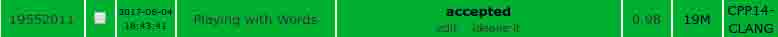
\includegraphics[scale=0.5]{assets/images/jpg/single-submission.jpg}}
  	\caption{Hasil uji coba pada situs penilaian SPOJ}
  	\label{figure:best_submission}
  \end{figure}
  
  \begin{figure}[H]
  	\centerline{ 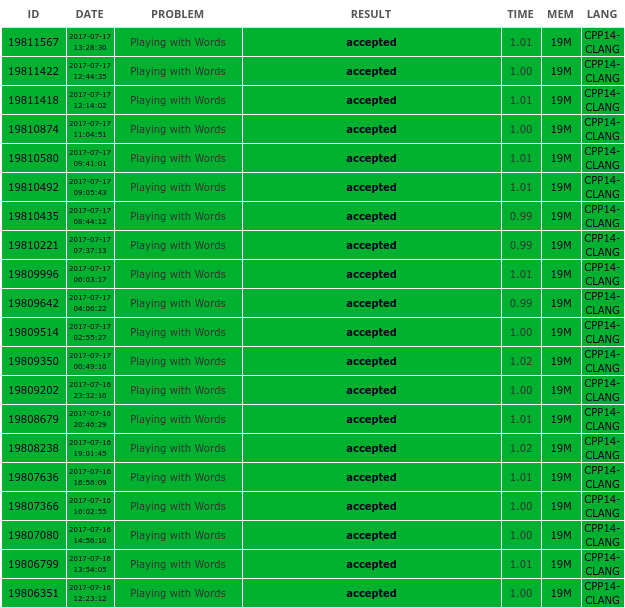
\includegraphics[scale=0.6]{assets/images/ujisubmission1.png}}
  	\caption{Hasil pengujian sebanyak 30 kali pada situs penilaian daring SPOJ (1)}
  	\label{figure:submission1}
  \end{figure}
  
  \begin{figure}[H]
  	\centerline{ 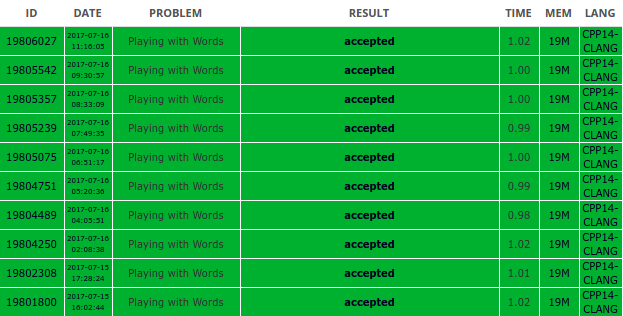
\includegraphics[scale=0.6]{assets/images/ujisubmission2.png}}
  	\caption{Hasil pengujian sebanyak 30 kali pada situs penilaian daring SPOJ (2)}
  	\label{figure:submission2}
  \end{figure}
  
  \begin{figure}[H]
  	\centerline{ 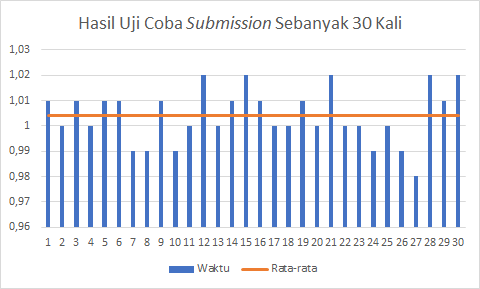
\includegraphics[scale=0.7]{assets/images/submission-chart.png}}
  	\caption{Grafik hasil uji coba pada situs SPOJ sebanyak 30 kali}
  	\label{figure:chart}
  \end{figure}
  
  \chapter{Tabel Simulasi Perhitungan Jumlah Kemungkinan \textit{String} orig1 dan orig2 pada Kasus \textit{String} ad1=c, \textit{String} ad2=n dan X=1}
  \setcounter{table}{0}
  \renewcommand{\thetable}{C.\arabic{table}}
  \renewcommand{\thefigure}{C.\arabic{figure}}
  
  % Iterasi dist = 0
  
  
  \begin{table}[H]
  	\centering
  	\begin{tabular} {|p{3cm}|p{5cm}|p{1cm}|} \hline
  		Fungsi & Perhitungan Nilai & Nilai \\ \hline
  		$ F_{(c, 0, 1)} $ & \textit{base case} & $ 1 $ \\ \hline
  		\rowcolor{LightCyan}
  		$ F_{(c, 1, 1)}  $ & $F_{(c, 0, 1)}$ & $ 1 $ \\ \hline
  	\end{tabular}\caption{Simulasi perhitungan jumlah kombinasi \textit{string} $ orig1 $ tanpa operasi \textit{replace} dengan $ dist= 0  $ pada kasus \textit{string} $ ad1=c $, \textit{string} $ ad2=n $ dan $ X=1 $}
  	\label{tab:f_2_orig1_0_1}
  \end{table}
  
  \begin{table}[H]
  	\centering
  	\begin{tabular} {|p{3cm}|p{5cm}|p{1cm}|} \hline
  		Fungsi & Perhitungan Nilai & Nilai \\ \hline
  		$ G_{(n, 0, 0)} $ & \textit{base case} & $ 0 $ \\ \hline
  		$ F_{(n, 0, 1)} $ & \textit{base case} & $ 1 $ \\ \hline
  		$ F_{(n, 0, 1)} $ & \textit{base case} & $ 1 $ \\ \hline
  		\rowcolor{LightCyan}
  		$ G_{(n, 1, 0)}  $ & $G_{(n, 0, 0)} + F_{(n, 0, 1)} + F_{(n, 0, 1)}$ & $ 2 $ \\ \hline
  	\end{tabular}\caption{Simulasi perhitungan jumlah kombinasi \textit{string} $ orig2 $ dengan operasi \textit{replace} dengan $ dist= 0  $ pada kasus \textit{string} $ ad1=c $, \textit{string} $ ad2=n $ dan $ X=1 $}
  	\label{tab:g_2_orig2_0_1}
  \end{table}
  
  \begin{table}[H]
  	\centering
  	\begin{tabular} {|p{3cm}|p{5cm}|p{1cm}|} \hline
  		Fungsi & Perhitungan Nilai & Nilai \\ \hline
  		$ G_{(c, 0, 1)} $ & \textit{base case} & $ 0 $ \\ \hline
  		$ F_{(c, 0, 2)} $ & \textit{base case} & $ 0 $ \\ \hline
  		$ F_{(c, 0, 2)} $ & \textit{base case} & $ 0 $ \\ \hline
  		\rowcolor{LightCyan}
  		$ G_{(c, 1, 1)}  $ & $G_{(c, 0, 1)} + F_{(c, 0, 2)} + F_{(c, 0, 2)}$ & $ 0 $ \\ \hline
  	\end{tabular}\caption{Simulasi perhitungan jumlah kombinasi \textit{string} $ orig1 $ dengan operasi \textit{replace} dengan $ dist= 0  $ pada kasus \textit{string} $ ad1=c $, \textit{string} $ ad2=n $ dan $ X=1 $}
  	\label{tab:g_2_orig1_0_1}
  \end{table}
  
  \begin{table}[H]
  	\centering
  	\begin{tabular} {|p{3cm}|p{5cm}|p{1cm}|} \hline
  		Fungsi & Perhitungan Nilai & Nilai \\ \hline
  		$ F_{(n, 0, 0)} $ & \textit{base case} & $ 0 $ \\ \hline
  		\rowcolor{LightCyan}
  		$ F_{(n, 1, 0)}  $ & $F_{(n, 0, 0)}$ & $ 0 $ \\ \hline
  	\end{tabular}\caption{Simulasi perhitungan jumlah kombinasi \textit{string} $ orig2 $ tanpa operasi \textit{replace} dengan $ dist= 0  $ pada kasus \textit{string} $ ad1=c $, \textit{string} $ ad2=n $ dan $ X=1 $}
  	\label{tab:f_2_orig2_0_1}
  \end{table}
  
  % Iterasi dist = 1
  
  
  \begin{table}[H]
  	\centering
  	\begin{tabular} {|p{3cm}|p{5cm}|p{1cm}|} \hline
  		Fungsi & Perhitungan Nilai & Nilai \\ \hline
  		$ F_{(c, 0, 0)} $ & \textit{base case} & $ 0 $ \\ \hline
  		\rowcolor{LightCyan}
  		$ F_{(c, 1, 0)}  $ & $F_{(c, 0, 0)}$ & $ 0 $ \\ \hline
  	\end{tabular}\caption{Simulasi perhitungan jumlah kombinasi \textit{string} $ orig1 $ tanpa operasi \textit{replace} dengan $ dist= 1  $ pada kasus \textit{string} $ ad1=c $, \textit{string} $ ad2=n $ dan $ X=1 $}
  	\label{tab:f_2_orig1_1_1}
  \end{table}
  
  \begin{table}[H]
  	\centering
  	\begin{tabular} {|p{3cm}|p{5cm}|p{1cm}|} \hline
  		Fungsi & Perhitungan Nilai & Nilai \\ \hline
  		$ G_{(n, 0, 1)} $ & \textit{base case} & $ 0 $ \\ \hline
  		$ F_{(n, 0, 2)} $ & \textit{base case} & $ 0 $ \\ \hline
  		$ F_{(n, 0, 2)} $ & \textit{base case} & $ 0 $ \\ \hline
  		\rowcolor{LightCyan}
  		$ G_{(n, 1, 1)}  $ & $G_{(n, 0, 1)} + F_{(n, 0, 2)} + F_{(n, 0, 2)}$ & $ 0 $ \\ \hline
  	\end{tabular}\caption{Simulasi perhitungan jumlah kombinasi \textit{string} $ orig2 $ dengan operasi \textit{replace} dengan $ dist= 1  $ pada kasus \textit{string} $ ad1=c $, \textit{string} $ ad2=n $ dan $ X=1 $}
  	\label{tab:g_2_orig2_1_1}
  \end{table}
  
  \begin{table}[H]
  	\centering
  	\begin{tabular} {|p{3cm}|p{5cm}|p{1cm}|} \hline
  		Fungsi & Perhitungan Nilai & Nilai \\ \hline
  		$ G_{(c, 0, 0)} $ & \textit{base case} & $ 0 $ \\ \hline
  		$ F_{(c, 0, 1)} $ & \textit{base case} & $ 1 $ \\ \hline
  		$ F_{(c, 0, 1)} $ & \textit{base case} & $ 1 $ \\ \hline
  		\rowcolor{LightCyan}
  		$ G_{(c, 1, 0)}  $ & $G_{(c, 0, 0)} + F_{(c, 0, 1)} + F_{(c, 0, 1)}$ & $ 2 $ \\ \hline
  	\end{tabular}\caption{Simulasi perhitungan jumlah kombinasi \textit{string} $ orig1 $ dengan operasi \textit{replace} dengan $ dist= 1  $ pada kasus \textit{string} $ ad1=c $, \textit{string} $ ad2=n $ dan $ X=1 $}
  	\label{tab:g_2_orig1_1_1}
  \end{table}
  
  \begin{table}[H]
  	\centering
  	\begin{tabular} {|p{3cm}|p{5cm}|p{1cm}|} \hline
  		Fungsi & Perhitungan Nilai & Nilai \\ \hline
  		$ F_{(n, 0, 1)} $ & \textit{base case} & $ 1 $ \\ \hline
  		\rowcolor{LightCyan}
  		$ F_{(n, 1, 1)}  $ & $F_{(n, 0, 1)}$ & $ 1 $ \\ \hline
  	\end{tabular}\caption{Simulasi perhitungan jumlah kombinasi \textit{string} $ orig2 $ tanpa operasi \textit{replace} dengan $ dist= 1  $ pada kasus \textit{string} $ ad1=c $, \textit{string} $ ad2=n $ dan $ X=1 $}
  	\label{tab:f_2_orig2_1_1}
  \end{table}
  
  \chapter{Tabel Simulasi Perhitungan Jumlah Kemungkinan \textit{String} orig1 dan orig2 pada Kasus \textit{String} ad1=kbenh, \textit{String} ad2=kbenh dan X=5}
  \setcounter{table}{0}
  \renewcommand{\thetable}{D.\arabic{table}}
  \renewcommand{\thefigure}{D.\arabic{figure}}
  
  % Iterasi dist = 0
  
  
  \begin{table}[H]
  	\centering
  	\begin{tabular} {|p{3cm}|p{5cm}|p{1cm}|} \hline
  		Fungsi & Perhitungan Nilai & Nilai \\ \hline
  		$ F_{(behkn, 0, 5)} $ & \textit{base case} & $ 1 $ \\ \hline
  		$ F_{(behkn, 16, 5)}  $ & $F_{(behkn, 0, 5)}$ & $ 1 $ \\ \hline
  		$ F_{(behkn, 8, 8)} $ & \textit{base case} & $ 0 $ \\ \hline
  		$ F_{(behkn, 24, 5)}  $ & $F_{(behkn, 16, 5)} + F_{(behkn, 8, 8)}$ & $ 1 $ \\ \hline
  		$ F_{(behkn, 20, 8)} $ & \textit{base case} & $ 0 $ \\ \hline
  		$ F_{(behkn, 12, 11)} $ & \textit{base case} & $ 0 $ \\ \hline
  		$ F_{(behkn, 28, 5)}  $ & $F_{(behkn, 24, 5)} + F_{(behkn, 20, 8)} + F_{(behkn, 12, 11)}$ & $ 1 $ \\ \hline
  		$ F_{(behkn, 26, 8)} $ & \textit{base case} & $ 0 $ \\ \hline
  		$ F_{(behkn, 22, 11)} $ & \textit{base case} & $ 0 $ \\ \hline
  		$ F_{(behkn, 14, 14)} $ & \textit{base case} & $ 0 $ \\ \hline
  		$ F_{(behkn, 30, 5)}  $ & $F_{(behkn, 28, 5)} + F_{(behkn, 26, 8)} + F_{(behkn, 22, 11)} + F_{(behkn, 14, 14)}$ & $ 1 $ \\ \hline
  		$ F_{(behkn, 29, 8)} $ & \textit{base case} & $ 0 $ \\ \hline
  		$ F_{(behkn, 27, 11)} $ & \textit{base case} & $ 0 $ \\ \hline
  		$ F_{(behkn, 23, 14)} $ & \textit{base case} & $ 0 $ \\ \hline
  	\end{tabular}\caption{Simulasi perhitungan jumlah kombinasi \textit{string} $ orig1 $ tanpa operasi \textit{replace} dengan $ dist= 0  $ pada kasus \textit{string} $ ad1=kbenh $, \textit{string} $ ad2=kbenh $ dan $ X=5 $}
  	\label{tab:f_3_orig1_0_1}
  \end{table}
  
  \begin{table}[H]
  	\centering
  	\begin{tabular} {|p{3cm}|p{5cm}|p{1cm}|} \hline
  		Fungsi & Perhitungan Nilai & Nilai \\ \hline  		
  		$ F_{(behkn, 15, 17)} $ & \textit{base case} & $ 0 $ \\ \hline
  		\rowcolor{LightCyan}
  		$ F_{(behkn, 31, 5)}  $ & $F_{(behkn, 30, 5)} + F_{(behkn, 29, 8)} + F_{(behkn, 27, 11)} + F_{(behkn, 23, 14)} + F_{(behkn, 15, 17)}$ & $ 1 $ \\ \hline
  	\end{tabular}\caption{Simulasi perhitungan jumlah kombinasi \textit{string} $ orig1 $ tanpa operasi \textit{replace} dengan $ dist= 0  $ pada kasus \textit{string} $ ad1=kbenh $, \textit{string} $ ad2=kbenh $ dan $ X=5 $}
  	\label{tab:f_3_orig1_0_2}
  \end{table}
  
  \begin{table}[H]
  	\centering
  	\begin{tabular} {|p{3cm}|p{5cm}|p{1cm}|} \hline
  		Fungsi & Perhitungan Nilai & Nilai \\ \hline
  		$ G_{(behkn, 0, 0)} $ & \textit{base case} & $ 0 $ \\ \hline
  		$ F_{(behkn, 0, 1)} $ & \textit{base case} & $ 0 $ \\ \hline
  		$ F_{(behkn, 0, 1)} $ & \textit{base case} & $ 0 $ \\ \hline
  		$ G_{(behkn, 16, 0)}  $ & $G_{(behkn, 0, 0)} + F_{(behkn, 0, 1)} + F_{(behkn, 0, 1)}$ & $ 0 $ \\ \hline
  		$ F_{(behkn, 0, 1)} $ & \textit{base case} & $ 0 $ \\ \hline
  		$ F_{(behkn, 16, 1)}  $ & $F_{(behkn, 0, 1)}$ & $ 0 $ \\ \hline
  		$ F_{(behkn, 16, 1)}  $ & $memoF_{(behkn, 16, 1)}$ & $ 0 $ \\ \hline
  		$ G_{(behkn, 0, 6)} $ & \textit{base case} & $ 0 $ \\ \hline
  		$ F_{(behkn, 0, 5)} $ & \textit{base case} & $ 1 $ \\ \hline
  		$ F_{(behkn, 0, 7)} $ & \textit{base case} & $ 0 $ \\ \hline
  		$ G_{(behkn, 8, 3)}  $ & $G_{(behkn, 0, 6)} + F_{(behkn, 0, 5)} + F_{(behkn, 0, 7)}$ & $ 1 $ \\ \hline
  		$ F_{(behkn, 0, 7)} $ & \textit{base case} & $ 0 $ \\ \hline
  		$ F_{(behkn, 8, 4)}  $ & $F_{(behkn, 0, 7)}$ & $ 0 $ \\ \hline
  		$ F_{(behkn, 0, 5)} $ & \textit{base case} & $ 1 $ \\ \hline
  		$ F_{(behkn, 8, 2)}  $ & $F_{(behkn, 0, 5)}$ & $ 1 $ \\ \hline
  		$ G_{(behkn, 24, 0)}  $ & $G_{(behkn, 16, 0)} + F_{(behkn, 16, 1)} + F_{(behkn, 16, 1)} + G_{(behkn, 8, 3)} + F_{(behkn, 8, 4)} + F_{(behkn, 8, 2)}$ & $ 2 $ \\ \hline
  		$ F_{(behkn, 16, 1)}  $ & $memoF_{(behkn, 16, 1)}$ & $ 0 $ \\ \hline
  		$ F_{(behkn, 8, 4)}  $ & $memoF_{(behkn, 8, 4)}$ & $ 0 $ \\ \hline
  		$ F_{(behkn, 24, 1)}  $ & $F_{(behkn, 16, 1)} + F_{(behkn, 8, 4)}$ & $ 0 $ \\ \hline
  		$ F_{(behkn, 24, 1)}  $ & $memoF_{(behkn, 24, 1)}$ & $ 0 $ \\ \hline
  		$ G_{(behkn, 16, 6)} $ & \textit{base case} & $ 0 $ \\ \hline
  		$ F_{(behkn, 0, 5)} $ & \textit{base case} & $ 1 $ \\ \hline
  		$ F_{(behkn, 16, 5)}  $ & $F_{(behkn, 0, 5)}$ & $ 1 $ \\ \hline
  		$ F_{(behkn, 16, 7)} $ & \textit{base case} & $ 0 $ \\ \hline
  	\end{tabular}\caption{Simulasi perhitungan jumlah kombinasi \textit{string} $ orig2 $ dengan operasi \textit{replace} dengan $ dist= 0  $ pada kasus \textit{string} $ ad1=kbenh $, \textit{string} $ ad2=kbenh $ dan $ X=5 $ (1)}
  	\label{tab:g_3_orig2_0_1}
  \end{table}
  \begin{table}[H]
  	\centering
  	\begin{tabular} {|p{3cm}|p{5cm}|p{1cm}|} \hline
  		Fungsi & Perhitungan Nilai & Nilai \\ \hline		
  		$ G_{(behkn, 4, 6)} $ & \textit{base case} & $ 0 $ \\ \hline
  		$ F_{(behkn, 4, 7)} $ & \textit{base case} & $ 0 $ \\ \hline
  		$ F_{(behkn, 0, 11)} $ & \textit{base case} & $ 0 $ \\ \hline
  		$ F_{(behkn, 4, 5)}  $ & $F_{(behkn, 0, 11)}$ & $ 0 $ \\ \hline
  		$ G_{(behkn, 20, 3)}  $ & $G_{(behkn, 16, 6)} + F_{(behkn, 16, 5)} + F_{(behkn, 16, 7)} + G_{(behkn, 4, 6)} + F_{(behkn, 4, 7)} + F_{(behkn, 4, 5)}$ & $ 1 $ \\ \hline
  		$ F_{(behkn, 16, 7)} $ & \textit{base case} & $ 0 $ \\ \hline
  		$ F_{(behkn, 4, 7)} $ & \textit{base case} & $ 0 $ \\ \hline
  		$ F_{(behkn, 20, 4)}  $ & $F_{(behkn, 16, 7)} + F_{(behkn, 4, 7)}$ & $ 0 $ \\ \hline
  		$ F_{(behkn, 16, 5)}  $ & $memoF_{(behkn, 16, 5)}$ & $ 1 $ \\ \hline
  		$ F_{(behkn, 4, 5)}  $ & $memoF_{(behkn, 4, 5)}$ & $ 0 $ \\ \hline
  		$ F_{(behkn, 20, 2)}  $ & $F_{(behkn, 16, 5)} + F_{(behkn, 4, 5)}$ & $ 1 $ \\ \hline
  		$ G_{(behkn, 12, 6)} $ & \textit{base case} & $ 0 $ \\ \hline
  		$ F_{(behkn, 12, 7)} $ & \textit{base case} & $ 0 $ \\ \hline
  		$ F_{(behkn, 8, 8)} $ & \textit{base case} & $ 0 $ \\ \hline
  		$ F_{(behkn, 4, 5)}  $ & $memoF_{(behkn, 4, 5)}$ & $ 0 $ \\ \hline
  		$ F_{(behkn, 12, 5)}  $ & $F_{(behkn, 8, 8)} + F_{(behkn, 4, 5)}$ & $ 0 $ \\ \hline
  		$ G_{(behkn, 28, 0)}  $ & $G_{(behkn, 24, 0)} + F_{(behkn, 24, 1)} + F_{(behkn, 24, 1)} + G_{(behkn, 20, 3)} + F_{(behkn, 20, 4)} + F_{(behkn, 20, 2)} + G_{(behkn, 12, 6)} + F_{(behkn, 12, 7)} + F_{(behkn, 12, 5)}$ & $ 4 $ \\ \hline
  		$ F_{(behkn, 24, 1)}  $ & $memoF_{(behkn, 24, 1)}$ & $ 0 $ \\ \hline
  		$ F_{(behkn, 20, 4)}  $ & $memoF_{(behkn, 20, 4)}$ & $ 0 $ \\ \hline
  		$ F_{(behkn, 12, 7)} $ & \textit{base case} & $ 0 $ \\ \hline
  		$ F_{(behkn, 28, 1)}  $ & $F_{(behkn, 24, 1)} + F_{(behkn, 20, 4)} + F_{(behkn, 12, 7)}$ & $ 0 $ \\ \hline
  	\end{tabular}\caption{Simulasi perhitungan jumlah kombinasi \textit{string} $ orig2 $ dengan operasi \textit{replace} dengan $ dist= 0  $ pada kasus \textit{string} $ ad1=kbenh $, \textit{string} $ ad2=kbenh $ dan $ X=5 $ (2)}
  	\label{tab:g_3_orig2_0_2}
  \end{table}
  \begin{table}[H]
  	\centering
  	\begin{tabular} {|p{3cm}|p{5cm}|p{1cm}|} \hline
  		Fungsi & Perhitungan Nilai & Nilai \\ \hline
  		
  		
  		$ F_{(behkn, 28, 1)}  $ & $memoF_{(behkn, 28, 1)}$ & $ 0 $ \\ \hline
  		$ G_{(behkn, 24, 6)} $ & \textit{base case} & $ 0 $ \\ \hline
  		$ F_{(behkn, 16, 5)}  $ & $memoF_{(behkn, 16, 5)}$ & $ 1 $ \\ \hline
  		$ F_{(behkn, 8, 8)} $ & \textit{base case} & $ 0 $ \\ \hline
  		$ F_{(behkn, 24, 5)}  $ & $F_{(behkn, 16, 5)} + F_{(behkn, 8, 8)}$ & $ 1 $ \\ \hline
  		$ F_{(behkn, 24, 7)} $ & \textit{base case} & $ 0 $ \\ \hline
  		$ G_{(behkn, 18, 6)} $ & \textit{base case} & $ 0 $ \\ \hline
  		$ F_{(behkn, 18, 7)} $ & \textit{base case} & $ 0 $ \\ \hline
  		$ F_{(behkn, 16, 11)} $ & \textit{base case} & $ 0 $ \\ \hline
  		$ F_{(behkn, 2, 8)} $ & \textit{base case} & $ 0 $ \\ \hline
  		$ F_{(behkn, 18, 5)}  $ & $F_{(behkn, 16, 11)} + F_{(behkn, 2, 8)}$ & $ 0 $ \\ \hline
  		$ G_{(behkn, 10, 9)} $ & \textit{base case} & $ 0 $ \\ \hline
  		$ F_{(behkn, 10, 10)} $ & \textit{base case} & $ 0 $ \\ \hline
  		$ F_{(behkn, 10, 8)} $ & \textit{base case} & $ 0 $ \\ \hline
  		$ G_{(behkn, 26, 3)}  $ & $G_{(behkn, 24, 6)} + F_{(behkn, 24, 5)} + F_{(behkn, 24, 7)} + G_{(behkn, 18, 6)} + F_{(behkn, 18, 7)} + F_{(behkn, 18, 5)} + G_{(behkn, 10, 9)} + F_{(behkn, 10, 10)} + F_{(behkn, 10, 8)}$ & $ 1 $ \\ \hline
  		$ F_{(behkn, 24, 7)} $ & \textit{base case} & $ 0 $ \\ \hline
  		$ F_{(behkn, 18, 7)} $ & \textit{base case} & $ 0 $ \\ \hline
  		$ F_{(behkn, 10, 10)} $ & \textit{base case} & $ 0 $ \\ \hline
  		$ F_{(behkn, 26, 4)}  $ & $F_{(behkn, 24, 7)} + F_{(behkn, 18, 7)} + F_{(behkn, 10, 10)}$ & $ 0 $ \\ \hline
  		$ F_{(behkn, 24, 5)}  $ & $memoF_{(behkn, 24, 5)}$ & $ 1 $ \\ \hline
  		$ F_{(behkn, 18, 5)}  $ & $memoF_{(behkn, 18, 5)}$ & $ 0 $ \\ \hline
  		$ F_{(behkn, 10, 8)} $ & \textit{base case} & $ 0 $ \\ \hline
  		$ F_{(behkn, 26, 2)}  $ & $F_{(behkn, 24, 5)} + F_{(behkn, 18, 5)} + F_{(behkn, 10, 8)}$ & $ 1 $ \\ \hline
  	\end{tabular}\caption{Simulasi perhitungan jumlah kombinasi \textit{string} $ orig2 $ dengan operasi \textit{replace} dengan $ dist= 0  $ pada kasus \textit{string} $ ad1=kbenh $, \textit{string} $ ad2=kbenh $ dan $ X=5 $ (3)}
  	\label{tab:g_3_orig2_0_3}
  \end{table}
  \begin{table}[H]
  	\centering
  	\begin{tabular} {|p{3cm}|p{5cm}|p{1cm}|} \hline
  		Fungsi & Perhitungan Nilai & Nilai \\ \hline
  		
  		$ G_{(behkn, 22, 6)} $ & \textit{base case} & $ 0 $ \\ \hline
  		$ F_{(behkn, 22, 7)} $ & \textit{base case} & $ 0 $ \\ \hline
  		$ F_{(behkn, 20, 8)} $ & \textit{base case} & $ 0 $ \\ \hline
  		$ F_{(behkn, 18, 5)}  $ & $memoF_{(behkn, 18, 5)}$ & $ 0 $ \\ \hline
  		$ F_{(behkn, 6, 11)} $ & \textit{base case} & $ 0 $ \\ \hline
  		$ F_{(behkn, 22, 5)}  $ & $F_{(behkn, 20, 8)} + F_{(behkn, 18, 5)} + F_{(behkn, 6, 11)}$ & $ 0 $ \\ \hline
  		$ G_{(behkn, 14, 9)} $ & \textit{base case} & $ 0 $ \\ \hline
  		$ F_{(behkn, 14, 10)} $ & \textit{base case} & $ 0 $ \\ \hline
  		$ F_{(behkn, 14, 8)} $ & \textit{base case} & $ 0 $ \\ \hline
  		$ G_{(behkn, 30, 0)}  $ & $G_{(behkn, 28, 0)} + F_{(behkn, 28, 1)} + F_{(behkn, 28, 1)} + G_{(behkn, 26, 3)} + F_{(behkn, 26, 4)} + F_{(behkn, 26, 2)} + G_{(behkn, 22, 6)} + F_{(behkn, 22, 7)} + F_{(behkn, 22, 5)} + G_{(behkn, 14, 9)} + F_{(behkn, 14, 10)} + F_{(behkn, 14, 8)}$ & $ 6 $ \\ \hline
  		$ F_{(behkn, 28, 1)}  $ & $memoF_{(behkn, 28, 1)}$ & $ 0 $ \\ \hline
  		$ F_{(behkn, 26, 4)}  $ & $memoF_{(behkn, 26, 4)}$ & $ 0 $ \\ \hline
  		$ F_{(behkn, 22, 7)} $ & \textit{base case} & $ 0 $ \\ \hline
  		$ F_{(behkn, 14, 10)} $ & \textit{base case} & $ 0 $ \\ \hline
  		$ F_{(behkn, 30, 1)}  $ & $F_{(behkn, 28, 1)} + F_{(behkn, 26, 4)} + F_{(behkn, 22, 7)} + F_{(behkn, 14, 10)}$ & $ 0 $ \\ \hline
  		$ F_{(behkn, 30, 1)}  $ & $memoF_{(behkn, 30, 1)}$ & $ 0 $ \\ \hline
  		$ G_{(behkn, 28, 6)} $ & \textit{base case} & $ 0 $ \\ \hline
  		$ F_{(behkn, 24, 5)}  $ & $memoF_{(behkn, 24, 5)}$ & $ 1 $ \\ \hline
  		$ F_{(behkn, 20, 8)} $ & \textit{base case} & $ 0 $ \\ \hline
  		$ F_{(behkn, 12, 11)} $ & \textit{base case} & $ 0 $ \\ \hline
  		$ F_{(behkn, 28, 5)}  $ & $F_{(behkn, 24, 5)} + F_{(behkn, 20, 8)} + F_{(behkn, 12, 11)}$ & $ 1 $ \\ \hline
  	\end{tabular}\caption{Simulasi perhitungan jumlah kombinasi \textit{string} $ orig2 $ dengan operasi \textit{replace} dengan $ dist= 0  $ pada kasus \textit{string} $ ad1=kbenh $, \textit{string} $ ad2=kbenh $ dan $ X=5 $ (4)}
  	\label{tab:g_3_orig2_0_4}
  \end{table}
  \begin{table}[H]
  	\centering
  	\begin{tabular} {|p{3cm}|p{5cm}|p{1cm}|} \hline
  		Fungsi & Perhitungan Nilai & Nilai \\ \hline
  		
  		$ F_{(behkn, 28, 7)} $ & \textit{base case} & $ 0 $ \\ \hline
  		$ G_{(behkn, 25, 6)} $ & \textit{base case} & $ 0 $ \\ \hline
  		$ F_{(behkn, 25, 7)} $ & \textit{base case} & $ 0 $ \\ \hline
  		$ F_{(behkn, 24, 11)} $ & \textit{base case} & $ 0 $ \\ \hline
  		$ F_{(behkn, 17, 8)} $ & \textit{base case} & $ 0 $ \\ \hline
  		$ F_{(behkn, 9, 11)} $ & \textit{base case} & $ 0 $ \\ \hline
  		$ F_{(behkn, 25, 5)}  $ & $F_{(behkn, 24, 11)} + F_{(behkn, 17, 8)} + F_{(behkn, 9, 11)}$ & $ 0 $ \\ \hline
  		$ G_{(behkn, 21, 9)} $ & \textit{base case} & $ 0 $ \\ \hline
  		$ F_{(behkn, 21, 10)} $ & \textit{base case} & $ 0 $ \\ \hline
  		$ F_{(behkn, 21, 8)} $ & \textit{base case} & $ 0 $ \\ \hline
  		$ G_{(behkn, 13, 12)} $ & \textit{base case} & $ 0 $ \\ \hline
  		$ F_{(behkn, 13, 13)} $ & \textit{base case} & $ 0 $ \\ \hline
  		$ F_{(behkn, 13, 11)} $ & \textit{base case} & $ 0 $ \\ \hline
  		$ G_{(behkn, 29, 3)}  $ & $G_{(behkn, 28, 6)} + F_{(behkn, 28, 5)} + F_{(behkn, 28, 7)} + G_{(behkn, 25, 6)} + F_{(behkn, 25, 7)} + F_{(behkn, 25, 5)} + G_{(behkn, 21, 9)} + F_{(behkn, 21, 10)} + F_{(behkn, 21, 8)} + G_{(behkn, 13, 12)} + F_{(behkn, 13, 13)} + F_{(behkn, 13, 11)}$ & $ 1 $ \\ \hline
  		$ F_{(behkn, 28, 7)} $ & \textit{base case} & $ 0 $ \\ \hline
  		$ F_{(behkn, 25, 7)} $ & \textit{base case} & $ 0 $ \\ \hline
  		$ F_{(behkn, 21, 10)} $ & \textit{base case} & $ 0 $ \\ \hline
  		$ F_{(behkn, 13, 13)} $ & \textit{base case} & $ 0 $ \\ \hline
  		$ F_{(behkn, 29, 4)}  $ & $F_{(behkn, 28, 7)} + F_{(behkn, 25, 7)} + F_{(behkn, 21, 10)} + F_{(behkn, 13, 13)}$ & $ 0 $ \\ \hline
  		$ F_{(behkn, 28, 5)}  $ & $memoF_{(behkn, 28, 5)}$ & $ 1 $ \\ \hline
  		$ F_{(behkn, 25, 5)}  $ & $memoF_{(behkn, 25, 5)}$ & $ 0 $ \\ \hline
  		$ F_{(behkn, 21, 8)} $ & \textit{base case} & $ 0 $ \\ \hline
  		$ F_{(behkn, 13, 11)} $ & \textit{base case} & $ 0 $ \\ \hline
  		
  		
  	\end{tabular}\caption{Simulasi perhitungan jumlah kombinasi \textit{string} $ orig2 $ dengan operasi \textit{replace} dengan $ dist= 0  $ pada kasus \textit{string} $ ad1=kbenh $, \textit{string} $ ad2=kbenh $ dan $ X=5 $ (5)}
  	\label{tab:g_3_orig2_0_5}
  \end{table}
  \begin{table}[H]
  	\centering
  	\begin{tabular} {|p{3cm}|p{5cm}|p{1cm}|} \hline
  		Fungsi & Perhitungan Nilai & Nilai \\ \hline
  		$ F_{(behkn, 27, 7)} $ & \textit{base case} & $ 0 $ \\ \hline
  		$ F_{(behkn, 26, 8)} $ & \textit{base case} & $ 0 $ \\ \hline
  		$ F_{(behkn, 25, 5)}  $ & $memoF_{(behkn, 25, 5)}$ & $ 0 $ \\ \hline
  		$ F_{(behkn, 19, 11)} $ & \textit{base case} & $ 0 $ \\ \hline
  		$ F_{(behkn, 11, 14)} $ & \textit{base case} & $ 0 $ \\ \hline
  		$ F_{(behkn, 27, 5)}  $ & $F_{(behkn, 26, 8)} + F_{(behkn, 25, 5)} + F_{(behkn, 19, 11)} + F_{(behkn, 11, 14)}$ & $ 0 $ \\ \hline
  		$ G_{(behkn, 23, 9)} $ & \textit{base case} & $ 0 $ \\ \hline
  		$ F_{(behkn, 23, 10)} $ & \textit{base case} & $ 0 $ \\ \hline
  		$ F_{(behkn, 23, 8)} $ & \textit{base case} & $ 0 $ \\ \hline
  		$ G_{(behkn, 15, 12)} $ & \textit{base case} & $ 0 $ \\ \hline
  		$ F_{(behkn, 15, 13)} $ & \textit{base case} & $ 0 $ \\ \hline
  		$ F_{(behkn, 15, 11)} $ & \textit{base case} & $ 0 $ \\ \hline
  		\rowcolor{LightCyan}
  		$ G_{(behkn, 31, 0)}  $ & $G_{(behkn, 30, 0)} + F_{(behkn, 30, 1)} + F_{(behkn, 30, 1)} + G_{(behkn, 29, 3)} + F_{(behkn, 29, 4)} + F_{(behkn, 29, 2)} + G_{(behkn, 27, 6)} + F_{(behkn, 27, 7)} + F_{(behkn, 27, 5)} + G_{(behkn, 23, 9)} + F_{(behkn, 23, 10)} + F_{(behkn, 23, 8)} + G_{(behkn, 15, 12)} + F_{(behkn, 15, 13)} + F_{(behkn, 15, 11)}$ & $ 8 $ \\ \hline
  	\end{tabular}\caption{Simulasi perhitungan jumlah kombinasi \textit{string} $ orig2 $ dengan operasi \textit{replace} dengan $ dist= 0  $ pada kasus \textit{string} $ ad1=kbenh $, \textit{string} $ ad2=kbenh $ dan $ X=5 $ (6)}
  	\label{tab:g_3_orig2_0_6}
  \end{table}
  
  \begin{table}[H]
  	\centering
  	\begin{tabular} {|p{3cm}|p{5cm}|p{1cm}|} \hline
  		Fungsi & Perhitungan Nilai & Nilai \\ \hline
  		$ G_{(behkn, 0, 5)} $ & \textit{base case} & $ 0 $ \\ \hline
  		$ F_{(behkn, 0, 6)} $ & \textit{base case} & $ 0 $ \\ \hline
  		$ F_{(behkn, 0, 6)} $ & \textit{base case} & $ 0 $ \\ \hline
  		$ G_{(behkn, 16, 5)}  $ & $G_{(behkn, 0, 5)} + F_{(behkn, 0, 6)} + F_{(behkn, 0, 6)}$ & $ 0 $ \\ \hline
  		$ F_{(behkn, 16, 6)} $ & \textit{base case} & $ 0 $ \\ \hline
  		$ F_{(behkn, 16, 6)} $ & \textit{base case} & $ 0 $ \\ \hline
  		$ G_{(behkn, 8, 8)} $ & \textit{base case} & $ 0 $ \\ \hline
  		$ F_{(behkn, 8, 9)} $ & \textit{base case} & $ 0 $ \\ \hline
  		$ F_{(behkn, 8, 7)} $ & \textit{base case} & $ 0 $ \\ \hline
  		$ G_{(behkn, 24, 5)}  $ & $G_{(behkn, 16, 5)} + F_{(behkn, 16, 6)} + F_{(behkn, 16, 6)} + G_{(behkn, 8, 8)} + F_{(behkn, 8, 9)} + F_{(behkn, 8, 7)}$ & $ 0 $ \\ \hline
  		$ F_{(behkn, 24, 6)} $ & \textit{base case} & $ 0 $ \\ \hline
  		$ F_{(behkn, 24, 6)} $ & \textit{base case} & $ 0 $ \\ \hline
  		$ G_{(behkn, 20, 8)} $ & \textit{base case} & $ 0 $ \\ \hline
  		$ F_{(behkn, 20, 9)} $ & \textit{base case} & $ 0 $ \\ \hline
  		$ F_{(behkn, 20, 7)} $ & \textit{base case} & $ 0 $ \\ \hline
  		$ G_{(behkn, 12, 11)} $ & \textit{base case} & $ 0 $ \\ \hline
  		$ F_{(behkn, 12, 12)} $ & \textit{base case} & $ 0 $ \\ \hline
  		$ F_{(behkn, 12, 10)} $ & \textit{base case} & $ 0 $ \\ \hline
  		$ G_{(behkn, 28, 5)}  $ & $G_{(behkn, 24, 5)} + F_{(behkn, 24, 6)} + F_{(behkn, 24, 6)} + G_{(behkn, 20, 8)} + F_{(behkn, 20, 9)} + F_{(behkn, 20, 7)} + G_{(behkn, 12, 11)} + F_{(behkn, 12, 12)} + F_{(behkn, 12, 10)}$ & $ 0 $ \\ \hline
  		$ F_{(behkn, 28, 6)} $ & \textit{base case} & $ 0 $ \\ \hline
  		$ F_{(behkn, 28, 6)} $ & \textit{base case} & $ 0 $ \\ \hline
  	\end{tabular}\caption{Simulasi perhitungan jumlah kombinasi \textit{string} $ orig1 $ dengan operasi \textit{replace} dengan $ dist= 0  $ pada kasus \textit{string} $ ad1=kbenh $, \textit{string} $ ad2=kbenh $ dan $ X=5 $ (1)}
  	\label{tab:g_3_orig1_0_1}
  \end{table}
  \begin{table}[H]
  	\centering
  	\begin{tabular} {|p{3cm}|p{5cm}|p{1cm}|} \hline
  		Fungsi & Perhitungan Nilai & Nilai \\ \hline		
  		$ G_{(behkn, 26, 8)} $ & \textit{base case} & $ 0 $ \\ \hline
  		$ F_{(behkn, 26, 9)} $ & \textit{base case} & $ 0 $ \\ \hline
  		$ F_{(behkn, 26, 7)} $ & \textit{base case} & $ 0 $ \\ \hline
  		$ G_{(behkn, 22, 11)} $ & \textit{base case} & $ 0 $ \\ \hline
  		$ F_{(behkn, 22, 12)} $ & \textit{base case} & $ 0 $ \\ \hline
  		$ F_{(behkn, 22, 10)} $ & \textit{base case} & $ 0 $ \\ \hline
  		$ G_{(behkn, 14, 14)} $ & \textit{base case} & $ 0 $ \\ \hline
  		$ F_{(behkn, 14, 15)} $ & \textit{base case} & $ 0 $ \\ \hline
  		$ F_{(behkn, 14, 13)} $ & \textit{base case} & $ 0 $ \\ \hline
  		$ G_{(behkn, 30, 5)}  $ & $G_{(behkn, 28, 5)} + F_{(behkn, 28, 6)} + F_{(behkn, 28, 6)} + G_{(behkn, 26, 8)} + F_{(behkn, 26, 9)} + F_{(behkn, 26, 7)} + G_{(behkn, 22, 11)} + F_{(behkn, 22, 12)} + F_{(behkn, 22, 10)} + G_{(behkn, 14, 14)} + F_{(behkn, 14, 15)} + F_{(behkn, 14, 13)}$ & $ 0 $ \\ \hline
  		$ F_{(behkn, 30, 6)} $ & \textit{base case} & $ 0 $ \\ \hline
  		$ F_{(behkn, 30, 6)} $ & \textit{base case} & $ 0 $ \\ \hline
  		$ G_{(behkn, 29, 8)} $ & \textit{base case} & $ 0 $ \\ \hline
  		$ F_{(behkn, 29, 9)} $ & \textit{base case} & $ 0 $ \\ \hline
  		$ F_{(behkn, 29, 7)} $ & \textit{base case} & $ 0 $ \\ \hline
  		$ G_{(behkn, 27, 11)} $ & \textit{base case} & $ 0 $ \\ \hline
  		$ F_{(behkn, 27, 12)} $ & \textit{base case} & $ 0 $ \\ \hline
  		$ F_{(behkn, 27, 10)} $ & \textit{base case} & $ 0 $ \\ \hline
  		$ G_{(behkn, 23, 14)} $ & \textit{base case} & $ 0 $ \\ \hline
  		$ F_{(behkn, 23, 15)} $ & \textit{base case} & $ 0 $ \\ \hline
  		$ F_{(behkn, 23, 13)} $ & \textit{base case} & $ 0 $ \\ \hline
  		$ G_{(behkn, 15, 17)} $ & \textit{base case} & $ 0 $ \\ \hline
  	\end{tabular}\caption{Simulasi perhitungan jumlah kombinasi \textit{string} $ orig1 $ dengan operasi \textit{replace} dengan $ dist= 0  $ pada kasus \textit{string} $ ad1=kbenh $, \textit{string} $ ad2=kbenh $ dan $ X=5 $ (2)}
  	\label{tab:g_3_orig1_0_2}
  \end{table}
  \begin{table}[H]
  	\centering
  	\begin{tabular} {|p{3cm}|p{5cm}|p{1cm}|} \hline
  		Fungsi & Perhitungan Nilai & Nilai \\ \hline
  		
  		$ F_{(behkn, 15, 18)} $ & \textit{base case} & $ 0 $ \\ \hline
  		$ F_{(behkn, 15, 16)} $ & \textit{base case} & $ 0 $ \\ \hline
  		\rowcolor{LightCyan}
  		$ G_{(behkn, 31, 5)}  $ & $G_{(behkn, 30, 5)} + F_{(behkn, 30, 6)} + F_{(behkn, 30, 6)} + G_{(behkn, 29, 8)} + F_{(behkn, 29, 9)} + F_{(behkn, 29, 7)} + G_{(behkn, 27, 11)} + F_{(behkn, 27, 12)} + F_{(behkn, 27, 10)} + G_{(behkn, 23, 14)} + F_{(behkn, 23, 15)} + F_{(behkn, 23, 13)} + G_{(behkn, 15, 17)} + F_{(behkn, 15, 18)} + F_{(behkn, 15, 16)}$ & $ 0 $ \\ \hline
  	\end{tabular}\caption{Simulasi perhitungan jumlah kombinasi \textit{string} $ orig1 $ dengan operasi \textit{replace} dengan $ dist= 0  $ pada kasus \textit{string} $ ad1=kbenh $, \textit{string} $ ad2=kbenh $ dan $ X=5 $ (3)}
  	\label{tab:g_3_orig1_0_3}
  \end{table}
  
  \begin{table}[H]
  	\centering
  	\begin{tabular} {|p{3cm}|p{5cm}|p{1cm}|} \hline
  		Fungsi & Perhitungan Nilai & Nilai \\ \hline
  		$ F_{(behkn, 0, 0)} $ & \textit{base case} & $ 0 $ \\ \hline
  		$ F_{(behkn, 16, 0)}  $ & $F_{(behkn, 0, 0)}$ & $ 0 $ \\ \hline
  		$ F_{(behkn, 0, 6)} $ & \textit{base case} & $ 0 $ \\ \hline
  		$ F_{(behkn, 8, 3)}  $ & $F_{(behkn, 0, 6)}$ & $ 0 $ \\ \hline
  		$ F_{(behkn, 24, 0)}  $ & $F_{(behkn, 16, 0)} + F_{(behkn, 8, 3)}$ & $ 0 $ \\ \hline
  		$ F_{(behkn, 16, 6)} $ & \textit{base case} & $ 0 $ \\ \hline
  		$ F_{(behkn, 4, 6)} $ & \textit{base case} & $ 0 $ \\ \hline
  		$ F_{(behkn, 20, 3)}  $ & $F_{(behkn, 16, 6)} + F_{(behkn, 4, 6)}$ & $ 0 $ \\ \hline
  		$ F_{(behkn, 12, 6)} $ & \textit{base case} & $ 0 $ \\ \hline
  		$ F_{(behkn, 28, 0)}  $ & $F_{(behkn, 24, 0)} + F_{(behkn, 20, 3)} + F_{(behkn, 12, 6)}$ & $ 0 $ \\ \hline
  		$ F_{(behkn, 24, 6)} $ & \textit{base case} & $ 0 $ \\ \hline
  		$ F_{(behkn, 18, 6)} $ & \textit{base case} & $ 0 $ \\ \hline
  		$ F_{(behkn, 10, 9)} $ & \textit{base case} & $ 0 $ \\ \hline
  		$ F_{(behkn, 26, 3)}  $ & $F_{(behkn, 24, 6)} + F_{(behkn, 18, 6)} + F_{(behkn, 10, 9)}$ & $ 0 $ \\ \hline
  		$ F_{(behkn, 22, 6)} $ & \textit{base case} & $ 0 $ \\ \hline
  		$ F_{(behkn, 14, 9)} $ & \textit{base case} & $ 0 $ \\ \hline
  		$ F_{(behkn, 30, 0)}  $ & $F_{(behkn, 28, 0)} + F_{(behkn, 26, 3)} + F_{(behkn, 22, 6)} + F_{(behkn, 14, 9)}$ & $ 0 $ \\ \hline
  		$ F_{(behkn, 28, 6)} $ & \textit{base case} & $ 0 $ \\ \hline
  		$ F_{(behkn, 25, 6)} $ & \textit{base case} & $ 0 $ \\ \hline
  		$ F_{(behkn, 21, 9)} $ & \textit{base case} & $ 0 $ \\ \hline
  		$ F_{(behkn, 13, 12)} $ & \textit{base case} & $ 0 $ \\ \hline
  		$ F_{(behkn, 29, 3)}  $ & $F_{(behkn, 28, 6)} + F_{(behkn, 25, 6)} + F_{(behkn, 21, 9)} + F_{(behkn, 13, 12)}$ & $ 0 $ \\ \hline
  	\end{tabular}\caption{Simulasi perhitungan jumlah kombinasi \textit{string} $ orig2 $ tanpa operasi \textit{replace} dengan $ dist= 0  $ pada kasus \textit{string} $ ad1=kbenh $, \textit{string} $ ad2=kbenh $ dan $ X=5 $ (1)}
  	\label{tab:f_3_orig2_0_1}
  \end{table}
  \begin{table}[H]
  	\centering
  	\begin{tabular} {|p{3cm}|p{5cm}|p{1cm}|} \hline
  		Fungsi & Perhitungan Nilai & Nilai \\ \hline		
  		
  		$ F_{(behkn, 27, 6)} $ & \textit{base case} & $ 0 $ \\ \hline
  		$ F_{(behkn, 23, 9)} $ & \textit{base case} & $ 0 $ \\ \hline
  		$ F_{(behkn, 15, 12)} $ & \textit{base case} & $ 0 $ \\ \hline
  		\rowcolor{LightCyan}
  		$ F_{(behkn, 31, 0)}  $ & $F_{(behkn, 30, 0)} + F_{(behkn, 29, 3)} + F_{(behkn, 27, 6)} + F_{(behkn, 23, 9)} + F_{(behkn, 15, 12)}$ & $ 0 $ \\ \hline
  	\end{tabular}\caption{Simulasi perhitungan jumlah kombinasi \textit{string} $ orig2 $ tanpa operasi \textit{replace} dengan $ dist= 0  $ pada kasus \textit{string} $ ad1=kbenh $, \textit{string} $ ad2=kbenh $ dan $ X=5 $ (2)}
  	\label{tab:f_3_orig2_0_2}
  \end{table}
  
  
  % -----------------------------------------------------
  % -----------------------------------------------------
  % -----------------------------------------------------
  % -----------------------------------------------------
  % -----------------------------------------------------
  % -----------------------------------------------------
  % -----------------------------------------------------
  % -----------------------------------------------------
  % -----------------------------------------------------
  % -----------------------------------------------------
  % -----------------------------------------------------
  % -----------------------------------------------------
  % -----------------------------------------------------
  % -----------------------------------------------------
  % -----------------------------------------------------
  % -----------------------------------------------------
  % -----------------------------------------------------
  % -----------------------------------------------------
  % -----------------------------------------------------
  % -----------------------------------------------------
  % -----------------------------------------------------
  % -----------------------------------------------------
  % -----------------------------------------------------
  % -----------------------------------------------------
  % -----------------------------------------------------
  % -----------------------------------------------------
  % -----------------------------------------------------
  % -----------------------------------------------------
  % -----------------------------------------------------
  % -----------------------------------------------------
  % -----------------------------------------------------
  % -----------------------------------------------------
  % -----------------------------------------------------
  
  % Iterasi dist = 1
  
  
  \begin{table}[H]
  	\centering
  	\begin{tabular} {|p{3cm}|p{5cm}|p{1cm}|} \hline
  		Fungsi & Perhitungan Nilai & Nilai \\ \hline
  		$ F_{(behkn, 0, 4)} $ & \textit{base case} & $ 0 $ \\ \hline
  		$ F_{(behkn, 16, 4)}  $ & $F_{(behkn, 0, 4)}$ & $ 0 $ \\ \hline
  		$ F_{(behkn, 8, 7)} $ & \textit{base case} & $ 0 $ \\ \hline
  		$ F_{(behkn, 24, 4)}  $ & $F_{(behkn, 16, 4)} + F_{(behkn, 8, 7)}$ & $ 0 $ \\ \hline
  		$ F_{(behkn, 20, 7)} $ & \textit{base case} & $ 0 $ \\ \hline
  		$ F_{(behkn, 12, 10)} $ & \textit{base case} & $ 0 $ \\ \hline
  		$ F_{(behkn, 28, 4)}  $ & $F_{(behkn, 24, 4)} + F_{(behkn, 20, 7)} + F_{(behkn, 12, 10)}$ & $ 0 $ \\ \hline
  		$ F_{(behkn, 26, 7)} $ & \textit{base case} & $ 0 $ \\ \hline
  		$ F_{(behkn, 22, 10)} $ & \textit{base case} & $ 0 $ \\ \hline
  		$ F_{(behkn, 14, 13)} $ & \textit{base case} & $ 0 $ \\ \hline
  		$ F_{(behkn, 30, 4)}  $ & $F_{(behkn, 28, 4)} + F_{(behkn, 26, 7)} + F_{(behkn, 22, 10)} + F_{(behkn, 14, 13)}$ & $ 0 $ \\ \hline
  		$ F_{(behkn, 29, 7)} $ & \textit{base case} & $ 0 $ \\ \hline
  		$ F_{(behkn, 27, 10)} $ & \textit{base case} & $ 0 $ \\ \hline
  		$ F_{(behkn, 23, 13)} $ & \textit{base case} & $ 0 $ \\ \hline
  		$ F_{(behkn, 15, 16)} $ & \textit{base case} & $ 0 $ \\ \hline
  		\rowcolor{LightCyan}
  		$ F_{(behkn, 31, 4)}  $ & $F_{(behkn, 30, 4)} + F_{(behkn, 29, 7)} + F_{(behkn, 27, 10)} + F_{(behkn, 23, 13)} + F_{(behkn, 15, 16)}$ & $ 0 $ \\ \hline
  	\end{tabular}\caption{Simulasi perhitungan jumlah kombinasi \textit{string} $ orig1 $ tanpa operasi \textit{replace} dengan $ dist= 1  $ pada kasus \textit{string} $ ad1=kbenh $, \textit{string} $ ad2=kbenh $ dan $ X=5 $}
  	\label{tab:f_3_orig1_1_1}
  \end{table}
  
  \begin{table}[H]
  	\centering
  	\begin{tabular} {|p{3cm}|p{5cm}|p{1cm}|} \hline
  		Fungsi & Perhitungan Nilai & Nilai \\ \hline
  		$ G_{(behkn, 0, 1)} $ & \textit{base case} & $ 0 $ \\ \hline
  		$ F_{(behkn, 0, 2)} $ & \textit{base case} & $ 0 $ \\ \hline
  		$ F_{(behkn, 0, 2)} $ & \textit{base case} & $ 0 $ \\ \hline
  		$ G_{(behkn, 16, 1)}  $ & $G_{(behkn, 0, 1)} + F_{(behkn, 0, 2)} + F_{(behkn, 0, 2)}$ & $ 0 $ \\ \hline
  		$ F_{(behkn, 0, 2)} $ & \textit{base case} & $ 0 $ \\ \hline
  		$ F_{(behkn, 16, 2)}  $ & $F_{(behkn, 0, 2)}$ & $ 0 $ \\ \hline
  		$ F_{(behkn, 16, 2)}  $ & $memoF_{(behkn, 16, 2)}$ & $ 0 $ \\ \hline
  		$ G_{(behkn, 0, 7)} $ & \textit{base case} & $ 0 $ \\ \hline
  		$ F_{(behkn, 0, 6)} $ & \textit{base case} & $ 0 $ \\ \hline
  		$ F_{(behkn, 0, 8)} $ & \textit{base case} & $ 0 $ \\ \hline
  		$ G_{(behkn, 8, 4)}  $ & $G_{(behkn, 0, 7)} + F_{(behkn, 0, 6)} + F_{(behkn, 0, 8)}$ & $ 0 $ \\ \hline
  		$ F_{(behkn, 0, 8)} $ & \textit{base case} & $ 0 $ \\ \hline
  		$ F_{(behkn, 8, 5)}  $ & $F_{(behkn, 0, 8)}$ & $ 0 $ \\ \hline
  		$ F_{(behkn, 8, 3)}  $ & $memoF_{(behkn, 8, 3)}$ & $ 0 $ \\ \hline
  		$ G_{(behkn, 24, 1)}  $ & $G_{(behkn, 16, 1)} + F_{(behkn, 16, 2)} + F_{(behkn, 16, 2)} + G_{(behkn, 8, 4)} + F_{(behkn, 8, 5)} + F_{(behkn, 8, 3)}$ & $ 0 $ \\ \hline
  		$ F_{(behkn, 16, 2)}  $ & $memoF_{(behkn, 16, 2)}$ & $ 0 $ \\ \hline
  		$ F_{(behkn, 8, 5)}  $ & $memoF_{(behkn, 8, 5)}$ & $ 0 $ \\ \hline
  		$ F_{(behkn, 24, 2)}  $ & $F_{(behkn, 16, 2)} + F_{(behkn, 8, 5)}$ & $ 0 $ \\ \hline
  		$ F_{(behkn, 24, 2)}  $ & $memoF_{(behkn, 24, 2)}$ & $ 0 $ \\ \hline
  		$ G_{(behkn, 16, 7)} $ & \textit{base case} & $ 0 $ \\ \hline
  		$ F_{(behkn, 16, 6)} $ & \textit{base case} & $ 0 $ \\ \hline
  		$ F_{(behkn, 16, 8)} $ & \textit{base case} & $ 0 $ \\ \hline
  	\end{tabular}\caption{Simulasi perhitungan jumlah kombinasi \textit{string} $ orig2 $ dengan operasi \textit{replace} dengan $ dist= 1  $ pada kasus \textit{string} $ ad1=kbenh $, \textit{string} $ ad2=kbenh $ dan $ X=5 $ (1)}
  	\label{tab:g_3_orig2_1_1}
  \end{table}
  \begin{table}[H]
  	\centering
  	\begin{tabular} {|p{3cm}|p{5cm}|p{1cm}|} \hline
  		Fungsi & Perhitungan Nilai & Nilai \\ \hline				
  		$ G_{(behkn, 4, 7)} $ & \textit{base case} & $ 0 $ \\ \hline
  		$ F_{(behkn, 4, 8)} $ & \textit{base case} & $ 0 $ \\ \hline
  		$ F_{(behkn, 4, 6)} $ & \textit{base case} & $ 0 $ \\ \hline
  		$ G_{(behkn, 20, 4)}  $ & $G_{(behkn, 16, 7)} + F_{(behkn, 16, 6)} + F_{(behkn, 16, 8)} + G_{(behkn, 4, 7)} + F_{(behkn, 4, 8)} + F_{(behkn, 4, 6)}$ & $ 0 $ \\ \hline
  		$ F_{(behkn, 16, 8)} $ & \textit{base case} & $ 0 $ \\ \hline
  		$ F_{(behkn, 4, 8)} $ & \textit{base case} & $ 0 $ \\ \hline
  		$ F_{(behkn, 20, 5)}  $ & $F_{(behkn, 16, 8)} + F_{(behkn, 4, 8)}$ & $ 0 $ \\ \hline
  		$ F_{(behkn, 20, 3)}  $ & $memoF_{(behkn, 20, 3)}$ & $ 0 $ \\ \hline
  		$ G_{(behkn, 12, 7)} $ & \textit{base case} & $ 0 $ \\ \hline
  		$ F_{(behkn, 12, 8)} $ & \textit{base case} & $ 0 $ \\ \hline
  		$ F_{(behkn, 12, 6)} $ & \textit{base case} & $ 0 $ \\ \hline
  		$ G_{(behkn, 28, 1)}  $ & $G_{(behkn, 24, 1)} + F_{(behkn, 24, 2)} + F_{(behkn, 24, 2)} + G_{(behkn, 20, 4)} + F_{(behkn, 20, 5)} + F_{(behkn, 20, 3)} + G_{(behkn, 12, 7)} + F_{(behkn, 12, 8)} + F_{(behkn, 12, 6)}$ & $ 0 $ \\ \hline
  		$ F_{(behkn, 24, 2)}  $ & $memoF_{(behkn, 24, 2)}$ & $ 0 $ \\ \hline
  		$ F_{(behkn, 20, 5)}  $ & $memoF_{(behkn, 20, 5)}$ & $ 0 $ \\ \hline
  		$ F_{(behkn, 12, 8)} $ & \textit{base case} & $ 0 $ \\ \hline
  		$ F_{(behkn, 28, 2)}  $ & $F_{(behkn, 24, 2)} + F_{(behkn, 20, 5)} + F_{(behkn, 12, 8)}$ & $ 0 $ \\ \hline
  		$ F_{(behkn, 28, 2)}  $ & $memoF_{(behkn, 28, 2)}$ & $ 0 $ \\ \hline
  		$ G_{(behkn, 24, 7)} $ & \textit{base case} & $ 0 $ \\ \hline
  		$ F_{(behkn, 24, 6)} $ & \textit{base case} & $ 0 $ \\ \hline
  		$ F_{(behkn, 24, 8)} $ & \textit{base case} & $ 0 $ \\ \hline
  		$ G_{(behkn, 18, 7)} $ & \textit{base case} & $ 0 $ \\ \hline
  	\end{tabular}\caption{Simulasi perhitungan jumlah kombinasi \textit{string} $ orig2 $ dengan operasi \textit{replace} dengan $ dist= 1  $ pada kasus \textit{string} $ ad1=kbenh $, \textit{string} $ ad2=kbenh $ dan $ X=5 $ (2)}
  	\label{tab:g_3_orig2_1_2}
  \end{table}
  \begin{table}[H]
  	\centering
  	\begin{tabular} {|p{3cm}|p{5cm}|p{1cm}|} \hline
  		Fungsi & Perhitungan Nilai & Nilai \\ \hline				
  		$ F_{(behkn, 18, 8)} $ & \textit{base case} & $ 0 $ \\ \hline
  		$ F_{(behkn, 18, 6)} $ & \textit{base case} & $ 0 $ \\ \hline
  		$ G_{(behkn, 10, 10)} $ & \textit{base case} & $ 0 $ \\ \hline
  		$ F_{(behkn, 10, 11)} $ & \textit{base case} & $ 0 $ \\ \hline
  		$ F_{(behkn, 10, 9)} $ & \textit{base case} & $ 0 $ \\ \hline
  		$ G_{(behkn, 26, 4)}  $ & $G_{(behkn, 24, 7)} + F_{(behkn, 24, 6)} + F_{(behkn, 24, 8)} + G_{(behkn, 18, 7)} + F_{(behkn, 18, 8)} + F_{(behkn, 18, 6)} + G_{(behkn, 10, 10)} + F_{(behkn, 10, 11)} + F_{(behkn, 10, 9)}$ & $ 0 $ \\ \hline
  		$ F_{(behkn, 24, 8)} $ & \textit{base case} & $ 0 $ \\ \hline
  		$ F_{(behkn, 18, 8)} $ & \textit{base case} & $ 0 $ \\ \hline
  		$ F_{(behkn, 10, 11)} $ & \textit{base case} & $ 0 $ \\ \hline
  		$ F_{(behkn, 26, 5)}  $ & $F_{(behkn, 24, 8)} + F_{(behkn, 18, 8)} + F_{(behkn, 10, 11)}$ & $ 0 $ \\ \hline
  		$ F_{(behkn, 26, 3)}  $ & $memoF_{(behkn, 26, 3)}$ & $ 0 $ \\ \hline
  		$ G_{(behkn, 22, 7)} $ & \textit{base case} & $ 0 $ \\ \hline
  		$ F_{(behkn, 22, 8)} $ & \textit{base case} & $ 0 $ \\ \hline
  		$ F_{(behkn, 22, 6)} $ & \textit{base case} & $ 0 $ \\ \hline
  		$ G_{(behkn, 14, 10)} $ & \textit{base case} & $ 0 $ \\ \hline
  		$ F_{(behkn, 14, 11)} $ & \textit{base case} & $ 0 $ \\ \hline
  		$ F_{(behkn, 14, 9)} $ & \textit{base case} & $ 0 $ \\ \hline
  		$ G_{(behkn, 30, 1)}  $ & $G_{(behkn, 28, 1)} + F_{(behkn, 28, 2)} + F_{(behkn, 28, 2)} + G_{(behkn, 26, 4)} + F_{(behkn, 26, 5)} + F_{(behkn, 26, 3)} + G_{(behkn, 22, 7)} + F_{(behkn, 22, 8)} + F_{(behkn, 22, 6)} + G_{(behkn, 14, 10)} + F_{(behkn, 14, 11)} + F_{(behkn, 14, 9)}$ & $ 0 $ \\ \hline
  	\end{tabular}\caption{Simulasi perhitungan jumlah kombinasi \textit{string} $ orig2 $ dengan operasi \textit{replace} dengan $ dist= 1  $ pada kasus \textit{string} $ ad1=kbenh $, \textit{string} $ ad2=kbenh $ dan $ X=5 $ (3)}
  	\label{tab:g_3_orig2_1_3}
  \end{table}
  \begin{table}[H]
  	\centering
  	\begin{tabular} {|p{3cm}|p{5cm}|p{1cm}|} \hline
  		Fungsi & Perhitungan Nilai & Nilai \\ \hline		
  		
  		$ F_{(behkn, 28, 2)}  $ & $memoF_{(behkn, 28, 2)}$ & $ 0 $ \\ \hline
  		$ F_{(behkn, 26, 5)}  $ & $memoF_{(behkn, 26, 5)}$ & $ 0 $ \\ \hline
  		$ F_{(behkn, 22, 8)} $ & \textit{base case} & $ 0 $ \\ \hline
  		$ F_{(behkn, 14, 11)} $ & \textit{base case} & $ 0 $ \\ \hline
  		$ F_{(behkn, 30, 2)}  $ & $F_{(behkn, 28, 2)} + F_{(behkn, 26, 5)} + F_{(behkn, 22, 8)} + F_{(behkn, 14, 11)}$ & $ 0 $ \\ \hline
  		$ F_{(behkn, 30, 2)}  $ & $memoF_{(behkn, 30, 2)}$ & $ 0 $ \\ \hline
  		$ G_{(behkn, 28, 7)} $ & \textit{base case} & $ 0 $ \\ \hline
  		$ F_{(behkn, 28, 6)} $ & \textit{base case} & $ 0 $ \\ \hline
  		$ F_{(behkn, 28, 8)} $ & \textit{base case} & $ 0 $ \\ \hline
  		$ G_{(behkn, 25, 7)} $ & \textit{base case} & $ 0 $ \\ \hline
  		$ F_{(behkn, 25, 8)} $ & \textit{base case} & $ 0 $ \\ \hline
  		$ F_{(behkn, 25, 6)} $ & \textit{base case} & $ 0 $ \\ \hline
  		$ G_{(behkn, 21, 10)} $ & \textit{base case} & $ 0 $ \\ \hline
  		$ F_{(behkn, 21, 11)} $ & \textit{base case} & $ 0 $ \\ \hline
  		$ F_{(behkn, 21, 9)} $ & \textit{base case} & $ 0 $ \\ \hline
  		$ G_{(behkn, 13, 13)} $ & \textit{base case} & $ 0 $ \\ \hline
  		$ F_{(behkn, 13, 14)} $ & \textit{base case} & $ 0 $ \\ \hline
  		$ F_{(behkn, 13, 12)} $ & \textit{base case} & $ 0 $ \\ \hline
  		$ G_{(behkn, 29, 4)}  $ & $G_{(behkn, 28, 7)} + F_{(behkn, 28, 6)} + F_{(behkn, 28, 8)} + G_{(behkn, 25, 7)} + F_{(behkn, 25, 8)} + F_{(behkn, 25, 6)} + G_{(behkn, 21, 10)} + F_{(behkn, 21, 11)} + F_{(behkn, 21, 9)} + G_{(behkn, 13, 13)} + F_{(behkn, 13, 14)} + F_{(behkn, 13, 12)}$ & $ 0 $ \\ \hline
  		$ F_{(behkn, 28, 8)} $ & \textit{base case} & $ 0 $ \\ \hline
  		$ F_{(behkn, 25, 8)} $ & \textit{base case} & $ 0 $ \\ \hline
  		$ F_{(behkn, 21, 11)} $ & \textit{base case} & $ 0 $ \\ \hline
  		
  	\end{tabular}\caption{Simulasi perhitungan jumlah kombinasi \textit{string} $ orig2 $ dengan operasi \textit{replace} dengan $ dist= 1  $ pada kasus \textit{string} $ ad1=kbenh $, \textit{string} $ ad2=kbenh $ dan $ X=5 $ (4)}
  	\label{tab:g_3_orig2_1_4}
  \end{table}
  \begin{table}[H]
  	\centering
  	\begin{tabular} {|p{3cm}|p{5cm}|p{1cm}|} \hline
  		Fungsi & Perhitungan Nilai & Nilai \\ \hline		
  		$ F_{(behkn, 13, 14)} $ & \textit{base case} & $ 0 $ \\ \hline
  		$ F_{(behkn, 29, 5)}  $ & $F_{(behkn, 28, 8)} + F_{(behkn, 25, 8)} + F_{(behkn, 21, 11)} + F_{(behkn, 13, 14)}$ & $ 0 $ \\ \hline
  		$ F_{(behkn, 29, 3)}  $ & $memoF_{(behkn, 29, 3)}$ & $ 0 $ \\ \hline
  		$ G_{(behkn, 27, 7)} $ & \textit{base case} & $ 0 $ \\ \hline
  		$ F_{(behkn, 27, 8)} $ & \textit{base case} & $ 0 $ \\ \hline
  		$ F_{(behkn, 27, 6)} $ & \textit{base case} & $ 0 $ \\ \hline
  		$ G_{(behkn, 23, 10)} $ & \textit{base case} & $ 0 $ \\ \hline
  		$ F_{(behkn, 23, 11)} $ & \textit{base case} & $ 0 $ \\ \hline
  		$ F_{(behkn, 23, 9)} $ & \textit{base case} & $ 0 $ \\ \hline
  		$ G_{(behkn, 15, 13)} $ & \textit{base case} & $ 0 $ \\ \hline
  		$ F_{(behkn, 15, 14)} $ & \textit{base case} & $ 0 $ \\ \hline
  		$ F_{(behkn, 15, 12)} $ & \textit{base case} & $ 0 $ \\ \hline
  		\rowcolor{LightCyan}
  		$ G_{(behkn, 31, 1)}  $ & $G_{(behkn, 30, 1)} + F_{(behkn, 30, 2)} + F_{(behkn, 30, 2)} + G_{(behkn, 29, 4)} + F_{(behkn, 29, 5)} + F_{(behkn, 29, 3)} + G_{(behkn, 27, 7)} + F_{(behkn, 27, 8)} + F_{(behkn, 27, 6)} + G_{(behkn, 23, 10)} + F_{(behkn, 23, 11)} + F_{(behkn, 23, 9)} + G_{(behkn, 15, 13)} + F_{(behkn, 15, 14)} + F_{(behkn, 15, 12)}$ & $ 0 $ \\ \hline
  	\end{tabular}\caption{Simulasi perhitungan jumlah kombinasi \textit{string} $ orig2 $ dengan operasi \textit{replace} dengan $ dist= 1  $ pada kasus \textit{string} $ ad1=kbenh $, \textit{string} $ ad2=kbenh $ dan $ X=5 $ (5)}
  	\label{tab:g_3_orig2_1_5}
  \end{table}
  
  \begin{table}[H]
  	\centering
  	\begin{tabular} {|p{3cm}|p{5cm}|p{1cm}|} \hline
  		Fungsi & Perhitungan Nilai & Nilai \\ \hline
  		$ G_{(behkn, 0, 4)} $ & \textit{base case} & $ 0 $ \\ \hline
  		$ F_{(behkn, 0, 5)} $ & \textit{base case} & $ 1 $ \\ \hline
  		$ F_{(behkn, 0, 5)} $ & \textit{base case} & $ 1 $ \\ \hline
  		$ G_{(behkn, 16, 4)}  $ & $G_{(behkn, 0, 4)} + F_{(behkn, 0, 5)} + F_{(behkn, 0, 5)}$ & $ 2 $ \\ \hline
  		$ F_{(behkn, 16, 5)}  $ & $memoF_{(behkn, 16, 5)}$ & $ 1 $ \\ \hline
  		$ F_{(behkn, 16, 5)}  $ & $memoF_{(behkn, 16, 5)}$ & $ 1 $ \\ \hline
  		$ G_{(behkn, 8, 7)} $ & \textit{base case} & $ 0 $ \\ \hline
  		$ F_{(behkn, 8, 8)} $ & \textit{base case} & $ 0 $ \\ \hline
  		$ F_{(behkn, 8, 6)} $ & \textit{base case} & $ 0 $ \\ \hline
  		$ G_{(behkn, 24, 4)}  $ & $G_{(behkn, 16, 4)} + F_{(behkn, 16, 5)} + F_{(behkn, 16, 5)} + G_{(behkn, 8, 7)} + F_{(behkn, 8, 8)} + F_{(behkn, 8, 6)}$ & $ 4 $ \\ \hline
  		$ F_{(behkn, 24, 5)}  $ & $memoF_{(behkn, 24, 5)}$ & $ 1 $ \\ \hline
  		$ F_{(behkn, 24, 5)}  $ & $memoF_{(behkn, 24, 5)}$ & $ 1 $ \\ \hline
  		$ G_{(behkn, 20, 7)} $ & \textit{base case} & $ 0 $ \\ \hline
  		$ F_{(behkn, 20, 8)} $ & \textit{base case} & $ 0 $ \\ \hline
  		$ F_{(behkn, 20, 6)} $ & \textit{base case} & $ 0 $ \\ \hline
  		$ G_{(behkn, 12, 10)} $ & \textit{base case} & $ 0 $ \\ \hline
  		$ F_{(behkn, 12, 11)} $ & \textit{base case} & $ 0 $ \\ \hline
  		$ F_{(behkn, 12, 9)} $ & \textit{base case} & $ 0 $ \\ \hline
  		$ G_{(behkn, 28, 4)}  $ & $G_{(behkn, 24, 4)} + F_{(behkn, 24, 5)} + F_{(behkn, 24, 5)} + G_{(behkn, 20, 7)} + F_{(behkn, 20, 8)} + F_{(behkn, 20, 6)} + G_{(behkn, 12, 10)} + F_{(behkn, 12, 11)} + F_{(behkn, 12, 9)}$ & $ 6 $ \\ \hline
  		$ F_{(behkn, 28, 5)}  $ & $memoF_{(behkn, 28, 5)}$ & $ 1 $ \\ \hline
  		$ F_{(behkn, 28, 5)}  $ & $memoF_{(behkn, 28, 5)}$ & $ 1 $ \\ \hline
  	\end{tabular}\caption{Simulasi perhitungan jumlah kombinasi \textit{string} $ orig1 $ dengan operasi \textit{replace} dengan $ dist= 1  $ pada kasus \textit{string} $ ad1=kbenh $, \textit{string} $ ad2=kbenh $ dan $ X=5 $ (1)}
  	\label{tab:g_3_orig1_1_1}
  \end{table}
  \begin{table}[H]
  	\centering
  	\begin{tabular} {|p{3cm}|p{5cm}|p{1cm}|} \hline
  		Fungsi & Perhitungan Nilai & Nilai \\ \hline		
  		
  		$ G_{(behkn, 26, 7)} $ & \textit{base case} & $ 0 $ \\ \hline
  		$ F_{(behkn, 26, 8)} $ & \textit{base case} & $ 0 $ \\ \hline
  		$ F_{(behkn, 26, 6)} $ & \textit{base case} & $ 0 $ \\ \hline
  		$ G_{(behkn, 22, 10)} $ & \textit{base case} & $ 0 $ \\ \hline
  		$ F_{(behkn, 22, 11)} $ & \textit{base case} & $ 0 $ \\ \hline
  		$ F_{(behkn, 22, 9)} $ & \textit{base case} & $ 0 $ \\ \hline
  		$ G_{(behkn, 14, 13)} $ & \textit{base case} & $ 0 $ \\ \hline
  		$ F_{(behkn, 14, 14)} $ & \textit{base case} & $ 0 $ \\ \hline
  		$ F_{(behkn, 14, 12)} $ & \textit{base case} & $ 0 $ \\ \hline
  		$ G_{(behkn, 30, 4)}  $ & $G_{(behkn, 28, 4)} + F_{(behkn, 28, 5)} + F_{(behkn, 28, 5)} + G_{(behkn, 26, 7)} + F_{(behkn, 26, 8)} + F_{(behkn, 26, 6)} + G_{(behkn, 22, 10)} + F_{(behkn, 22, 11)} + F_{(behkn, 22, 9)} + G_{(behkn, 14, 13)} + F_{(behkn, 14, 14)} + F_{(behkn, 14, 12)}$ & $ 8 $ \\ \hline
  		$ F_{(behkn, 30, 5)}  $ & $memoF_{(behkn, 30, 5)}$ & $ 1 $ \\ \hline
  		$ F_{(behkn, 30, 5)}  $ & $memoF_{(behkn, 30, 5)}$ & $ 1 $ \\ \hline
  		$ G_{(behkn, 29, 7)} $ & \textit{base case} & $ 0 $ \\ \hline
  		$ F_{(behkn, 29, 8)} $ & \textit{base case} & $ 0 $ \\ \hline
  		$ F_{(behkn, 29, 6)} $ & \textit{base case} & $ 0 $ \\ \hline
  		$ G_{(behkn, 27, 10)} $ & \textit{base case} & $ 0 $ \\ \hline
  		$ F_{(behkn, 27, 11)} $ & \textit{base case} & $ 0 $ \\ \hline
  		$ F_{(behkn, 27, 9)} $ & \textit{base case} & $ 0 $ \\ \hline
  		$ G_{(behkn, 23, 13)} $ & \textit{base case} & $ 0 $ \\ \hline
  		$ F_{(behkn, 23, 14)} $ & \textit{base case} & $ 0 $ \\ \hline
  		$ F_{(behkn, 23, 12)} $ & \textit{base case} & $ 0 $ \\ \hline
  		$ G_{(behkn, 15, 16)} $ & \textit{base case} & $ 0 $ \\ \hline
  		$ F_{(behkn, 15, 17)} $ & \textit{base case} & $ 0 $ \\ \hline
  	\end{tabular}\caption{Simulasi perhitungan jumlah kombinasi \textit{string} $ orig1 $ dengan operasi \textit{replace} dengan $ dist= 1  $ pada kasus \textit{string} $ ad1=kbenh $, \textit{string} $ ad2=kbenh $ dan $ X=5 $ (2)}
  	\label{tab:g_3_orig1_1_2}
  \end{table}
  \begin{table}[H]
  	\centering
  	\begin{tabular} {|p{3cm}|p{5cm}|p{1cm}|} \hline
  		Fungsi & Perhitungan Nilai & Nilai \\ \hline		
  		
  		$ F_{(behkn, 15, 15)} $ & \textit{base case} & $ 0 $ \\ \hline
  		\rowcolor{LightCyan}
  		$ G_{(behkn, 31, 4)}  $ & $G_{(behkn, 30, 4)} + F_{(behkn, 30, 5)} + F_{(behkn, 30, 5)} + G_{(behkn, 29, 7)} + F_{(behkn, 29, 8)} + F_{(behkn, 29, 6)} + G_{(behkn, 27, 10)} + F_{(behkn, 27, 11)} + F_{(behkn, 27, 9)} + G_{(behkn, 23, 13)} + F_{(behkn, 23, 14)} + F_{(behkn, 23, 12)} + G_{(behkn, 15, 16)} + F_{(behkn, 15, 17)} + F_{(behkn, 15, 15)}$ & $ 10 $ \\ \hline
  	\end{tabular}\caption{Simulasi perhitungan jumlah kombinasi \textit{string} $ orig1 $ dengan operasi \textit{replace} dengan $ dist= 1  $ pada kasus \textit{string} $ ad1=kbenh $, \textit{string} $ ad2=kbenh $ dan $ X=5 $ (3)}
  	\label{tab:g_3_orig1_1_3}
  \end{table}
  
  \begin{table}[H]
  	\centering
  	\begin{tabular} {|p{3cm}|p{5cm}|p{1cm}|} \hline
  		Fungsi & Perhitungan Nilai & Nilai \\ \hline
  		$ F_{(behkn, 30, 1)}  $ & $memoF_{(behkn, 30, 1)}$ & $ 0 $ \\ \hline
  		$ F_{(behkn, 29, 4)}  $ & $memoF_{(behkn, 29, 4)}$ & $ 0 $ \\ \hline
  		$ F_{(behkn, 27, 7)} $ & \textit{base case} & $ 0 $ \\ \hline
  		$ F_{(behkn, 23, 10)} $ & \textit{base case} & $ 0 $ \\ \hline
  		$ F_{(behkn, 15, 13)} $ & \textit{base case} & $ 0 $ \\ \hline
  		\rowcolor{LightCyan}
  		$ F_{(behkn, 31, 1)}  $ & $F_{(behkn, 30, 1)} + F_{(behkn, 29, 4)} + F_{(behkn, 27, 7)} + F_{(behkn, 23, 10)} + F_{(behkn, 15, 13)}$ & $ 0 $ \\ \hline
  	\end{tabular}\caption{Simulasi perhitungan jumlah kombinasi \textit{string} $ orig2 $ tanpa operasi \textit{replace} dengan $ dist= 1  $ pada kasus \textit{string} $ ad1=kbenh $, \textit{string} $ ad2=kbenh $ dan $ X=5 $}
  	\label{tab:f_3_orig2_1_1}
  \end{table}
  
  % -----------------------------------------------------
  % -----------------------------------------------------
  % -----------------------------------------------------
  % -----------------------------------------------------
  % -----------------------------------------------------
  % -----------------------------------------------------
  % -----------------------------------------------------
  % -----------------------------------------------------
  % -----------------------------------------------------
  % -----------------------------------------------------
  % -----------------------------------------------------
  % -----------------------------------------------------
  % -----------------------------------------------------
  % -----------------------------------------------------
  % -----------------------------------------------------
  % -----------------------------------------------------
  % -----------------------------------------------------
  % -----------------------------------------------------
  % -----------------------------------------------------
  % -----------------------------------------------------
  % -----------------------------------------------------
  % -----------------------------------------------------
  
  % Iterasi dist = 2
  
  
  \begin{table}[H]
  	\centering
  	\begin{tabular} {|p{3cm}|p{5cm}|p{1cm}|} \hline
  		Fungsi & Perhitungan Nilai & Nilai \\ \hline
  		$ F_{(behkn, 0, 3)} $ & \textit{base case} & $ 0 $ \\ \hline
  		$ F_{(behkn, 16, 3)}  $ & $F_{(behkn, 0, 3)}$ & $ 0 $ \\ \hline
  		$ F_{(behkn, 8, 6)} $ & \textit{base case} & $ 0 $ \\ \hline
  		$ F_{(behkn, 24, 3)}  $ & $F_{(behkn, 16, 3)} + F_{(behkn, 8, 6)}$ & $ 0 $ \\ \hline
  		$ F_{(behkn, 20, 6)} $ & \textit{base case} & $ 0 $ \\ \hline
  		$ F_{(behkn, 12, 9)} $ & \textit{base case} & $ 0 $ \\ \hline
  		$ F_{(behkn, 28, 3)}  $ & $F_{(behkn, 24, 3)} + F_{(behkn, 20, 6)} + F_{(behkn, 12, 9)}$ & $ 0 $ \\ \hline
  		$ F_{(behkn, 26, 6)} $ & \textit{base case} & $ 0 $ \\ \hline
  		$ F_{(behkn, 22, 9)} $ & \textit{base case} & $ 0 $ \\ \hline
  		$ F_{(behkn, 14, 12)} $ & \textit{base case} & $ 0 $ \\ \hline
  		$ F_{(behkn, 30, 3)}  $ & $F_{(behkn, 28, 3)} + F_{(behkn, 26, 6)} + F_{(behkn, 22, 9)} + F_{(behkn, 14, 12)}$ & $ 0 $ \\ \hline
  		$ F_{(behkn, 29, 6)} $ & \textit{base case} & $ 0 $ \\ \hline
  		$ F_{(behkn, 27, 9)} $ & \textit{base case} & $ 0 $ \\ \hline
  		$ F_{(behkn, 23, 12)} $ & \textit{base case} & $ 0 $ \\ \hline
  		$ F_{(behkn, 15, 15)} $ & \textit{base case} & $ 0 $ \\ \hline
  		\rowcolor{LightCyan}
  		$ F_{(behkn, 31, 3)}  $ & $F_{(behkn, 30, 3)} + F_{(behkn, 29, 6)} + F_{(behkn, 27, 9)} + F_{(behkn, 23, 12)} + F_{(behkn, 15, 15)}$ & $ 0 $ \\ \hline
  	\end{tabular}\caption{Simulasi perhitungan jumlah kombinasi \textit{string} $ orig1 $ tanpa operasi \textit{replace} dengan $ dist= 2  $ pada kasus \textit{string} $ ad1=kbenh $, \textit{string} $ ad2=kbenh $ dan $ X=5 $}
  	\label{tab:f_3_orig1_2_1}
  \end{table}
  
  \begin{table}[H]
  	\centering
  	\begin{tabular} {|p{3cm}|p{5cm}|p{1cm}|} \hline
  		Fungsi & Perhitungan Nilai & Nilai \\ \hline
  		$ G_{(behkn, 0, 2)} $ & \textit{base case} & $ 0 $ \\ \hline
  		$ F_{(behkn, 0, 3)} $ & \textit{base case} & $ 0 $ \\ \hline
  		$ F_{(behkn, 0, 3)} $ & \textit{base case} & $ 0 $ \\ \hline
  		$ G_{(behkn, 16, 2)}  $ & $G_{(behkn, 0, 2)} + F_{(behkn, 0, 3)} + F_{(behkn, 0, 3)}$ & $ 0 $ \\ \hline
  		$ F_{(behkn, 0, 3)} $ & \textit{base case} & $ 0 $ \\ \hline
  		$ F_{(behkn, 16, 3)}  $ & $F_{(behkn, 0, 3)}$ & $ 0 $ \\ \hline
  		$ F_{(behkn, 16, 3)}  $ & $memoF_{(behkn, 16, 3)}$ & $ 0 $ \\ \hline
  		$ G_{(behkn, 0, 8)} $ & \textit{base case} & $ 0 $ \\ \hline
  		$ F_{(behkn, 0, 7)} $ & \textit{base case} & $ 0 $ \\ \hline
  		$ F_{(behkn, 0, 9)} $ & \textit{base case} & $ 0 $ \\ \hline
  		$ G_{(behkn, 8, 5)}  $ & $G_{(behkn, 0, 8)} + F_{(behkn, 0, 7)} + F_{(behkn, 0, 9)}$ & $ 0 $ \\ \hline
  		$ F_{(behkn, 8, 6)} $ & \textit{base case} & $ 0 $ \\ \hline
  		$ F_{(behkn, 8, 4)}  $ & $memoF_{(behkn, 8, 4)}$ & $ 0 $ \\ \hline
  		$ G_{(behkn, 24, 2)}  $ & $G_{(behkn, 16, 2)} + F_{(behkn, 16, 3)} + F_{(behkn, 16, 3)} + G_{(behkn, 8, 5)} + F_{(behkn, 8, 6)} + F_{(behkn, 8, 4)}$ & $ 0 $ \\ \hline
  		$ F_{(behkn, 16, 3)}  $ & $memoF_{(behkn, 16, 3)}$ & $ 0 $ \\ \hline
  		$ F_{(behkn, 8, 6)} $ & \textit{base case} & $ 0 $ \\ \hline
  		$ F_{(behkn, 24, 3)}  $ & $F_{(behkn, 16, 3)} + F_{(behkn, 8, 6)}$ & $ 0 $ \\ \hline
  		$ F_{(behkn, 24, 3)}  $ & $memoF_{(behkn, 24, 3)}$ & $ 0 $ \\ \hline
  		$ G_{(behkn, 16, 8)} $ & \textit{base case} & $ 0 $ \\ \hline
  		$ F_{(behkn, 16, 7)} $ & \textit{base case} & $ 0 $ \\ \hline
  		$ F_{(behkn, 16, 9)} $ & \textit{base case} & $ 0 $ \\ \hline
  		$ G_{(behkn, 4, 8)} $ & \textit{base case} & $ 0 $ \\ \hline
  	\end{tabular}\caption{Simulasi perhitungan jumlah kombinasi \textit{string} $ orig2 $ dengan operasi \textit{replace} dengan $ dist= 2  $ pada kasus \textit{string} $ ad1=kbenh $, \textit{string} $ ad2=kbenh $ dan $ X=5 $ (1)}
  	\label{tab:g_3_orig2_2_1}
  \end{table}
  \begin{table}[H]
  	\centering
  	\begin{tabular} {|p{3cm}|p{5cm}|p{1cm}|} \hline
  		Fungsi & Perhitungan Nilai & Nilai \\ \hline
  		$ F_{(behkn, 4, 9)} $ & \textit{base case} & $ 0 $ \\ \hline
  		$ F_{(behkn, 4, 7)} $ & \textit{base case} & $ 0 $ \\ \hline
  		$ G_{(behkn, 20, 5)}  $ & $G_{(behkn, 16, 8)} + F_{(behkn, 16, 7)} + F_{(behkn, 16, 9)} + G_{(behkn, 4, 8)} + F_{(behkn, 4, 9)} + F_{(behkn, 4, 7)}$ & $ 0 $ \\ \hline
  		$ F_{(behkn, 20, 6)} $ & \textit{base case} & $ 0 $ \\ \hline
  		$ F_{(behkn, 20, 4)}  $ & $memoF_{(behkn, 20, 4)}$ & $ 0 $ \\ \hline
  		$ G_{(behkn, 12, 8)} $ & \textit{base case} & $ 0 $ \\ \hline
  		$ F_{(behkn, 12, 9)} $ & \textit{base case} & $ 0 $ \\ \hline
  		$ F_{(behkn, 12, 7)} $ & \textit{base case} & $ 0 $ \\ \hline
  		$ G_{(behkn, 28, 2)}  $ & $G_{(behkn, 24, 2)} + F_{(behkn, 24, 3)} + F_{(behkn, 24, 3)} + G_{(behkn, 20, 5)} + F_{(behkn, 20, 6)} + F_{(behkn, 20, 4)} + G_{(behkn, 12, 8)} + F_{(behkn, 12, 9)} + F_{(behkn, 12, 7)}$ & $ 0 $ \\ \hline
  		$ F_{(behkn, 24, 3)}  $ & $memoF_{(behkn, 24, 3)}$ & $ 0 $ \\ \hline
  		$ F_{(behkn, 20, 6)} $ & \textit{base case} & $ 0 $ \\ \hline
  		$ F_{(behkn, 12, 9)} $ & \textit{base case} & $ 0 $ \\ \hline
  		$ F_{(behkn, 28, 3)}  $ & $F_{(behkn, 24, 3)} + F_{(behkn, 20, 6)} + F_{(behkn, 12, 9)}$ & $ 0 $ \\ \hline
  		$ F_{(behkn, 28, 3)}  $ & $memoF_{(behkn, 28, 3)}$ & $ 0 $ \\ \hline
  		$ G_{(behkn, 24, 8)} $ & \textit{base case} & $ 0 $ \\ \hline
  		$ F_{(behkn, 24, 7)} $ & \textit{base case} & $ 0 $ \\ \hline
  		$ F_{(behkn, 24, 9)} $ & \textit{base case} & $ 0 $ \\ \hline
  		$ G_{(behkn, 18, 8)} $ & \textit{base case} & $ 0 $ \\ \hline
  		$ F_{(behkn, 18, 9)} $ & \textit{base case} & $ 0 $ \\ \hline
  		$ F_{(behkn, 18, 7)} $ & \textit{base case} & $ 0 $ \\ \hline
  		
  	\end{tabular}\caption{Simulasi perhitungan jumlah kombinasi \textit{string} $ orig2 $ dengan operasi \textit{replace} dengan $ dist= 2  $ pada kasus \textit{string} $ ad1=kbenh $, \textit{string} $ ad2=kbenh $ dan $ X=5 $ (2)}
  	\label{tab:g_3_orig2_2_2}
  \end{table}
  \begin{table}[H]
  	\centering
  	\begin{tabular} {|p{3cm}|p{5cm}|p{1cm}|} \hline
  		Fungsi & Perhitungan Nilai & Nilai \\ \hline
  		
  		$ G_{(behkn, 10, 11)} $ & \textit{base case} & $ 0 $ \\ \hline
  		$ F_{(behkn, 10, 12)} $ & \textit{base case} & $ 0 $ \\ \hline
  		$ F_{(behkn, 10, 10)} $ & \textit{base case} & $ 0 $ \\ \hline
  		$ G_{(behkn, 26, 5)}  $ & $G_{(behkn, 24, 8)} + F_{(behkn, 24, 7)} + F_{(behkn, 24, 9)} + G_{(behkn, 18, 8)} + F_{(behkn, 18, 9)} + F_{(behkn, 18, 7)} + G_{(behkn, 10, 11)} + F_{(behkn, 10, 12)} + F_{(behkn, 10, 10)}$ & $ 0 $ \\ \hline
  		$ F_{(behkn, 26, 6)} $ & \textit{base case} & $ 0 $ \\ \hline
  		$ F_{(behkn, 26, 4)}  $ & $memoF_{(behkn, 26, 4)}$ & $ 0 $ \\ \hline
  		$ G_{(behkn, 22, 8)} $ & \textit{base case} & $ 0 $ \\ \hline
  		$ F_{(behkn, 22, 9)} $ & \textit{base case} & $ 0 $ \\ \hline
  		$ F_{(behkn, 22, 7)} $ & \textit{base case} & $ 0 $ \\ \hline
  		$ G_{(behkn, 14, 11)} $ & \textit{base case} & $ 0 $ \\ \hline
  		$ F_{(behkn, 14, 12)} $ & \textit{base case} & $ 0 $ \\ \hline
  		$ F_{(behkn, 14, 10)} $ & \textit{base case} & $ 0 $ \\ \hline
  		$ G_{(behkn, 30, 2)}  $ & $G_{(behkn, 28, 2)} + F_{(behkn, 28, 3)} + F_{(behkn, 28, 3)} + G_{(behkn, 26, 5)} + F_{(behkn, 26, 6)} + F_{(behkn, 26, 4)} + G_{(behkn, 22, 8)} + F_{(behkn, 22, 9)} + F_{(behkn, 22, 7)} + G_{(behkn, 14, 11)} + F_{(behkn, 14, 12)} + F_{(behkn, 14, 10)}$ & $ 0 $ \\ \hline
  		$ F_{(behkn, 28, 3)}  $ & $memoF_{(behkn, 28, 3)}$ & $ 0 $ \\ \hline
  		$ F_{(behkn, 26, 6)} $ & \textit{base case} & $ 0 $ \\ \hline
  		$ F_{(behkn, 22, 9)} $ & \textit{base case} & $ 0 $ \\ \hline
  		$ F_{(behkn, 14, 12)} $ & \textit{base case} & $ 0 $ \\ \hline
  		$ F_{(behkn, 30, 3)}  $ & $F_{(behkn, 28, 3)} + F_{(behkn, 26, 6)} + F_{(behkn, 22, 9)} + F_{(behkn, 14, 12)}$ & $ 0 $ \\ \hline
  		
  	\end{tabular}\caption{Simulasi perhitungan jumlah kombinasi \textit{string} $ orig2 $ dengan operasi \textit{replace} dengan $ dist= 2  $ pada kasus \textit{string} $ ad1=kbenh $, \textit{string} $ ad2=kbenh $ dan $ X=5 $ (3)}
  	\label{tab:g_3_orig2_2_3}
  \end{table}
  \begin{table}[H]
  	\centering
  	\begin{tabular} {|p{3cm}|p{5cm}|p{1cm}|} \hline
  		Fungsi & Perhitungan Nilai & Nilai \\ \hline
  		$ F_{(behkn, 30, 3)}  $ & $memoF_{(behkn, 30, 3)}$ & $ 0 $ \\ \hline		
  		$ G_{(behkn, 28, 8)} $ & \textit{base case} & $ 0 $ \\ \hline
  		$ F_{(behkn, 28, 7)} $ & \textit{base case} & $ 0 $ \\ \hline
  		$ F_{(behkn, 28, 9)} $ & \textit{base case} & $ 0 $ \\ \hline
  		$ G_{(behkn, 25, 8)} $ & \textit{base case} & $ 0 $ \\ \hline
  		$ F_{(behkn, 25, 9)} $ & \textit{base case} & $ 0 $ \\ \hline
  		$ F_{(behkn, 25, 7)} $ & \textit{base case} & $ 0 $ \\ \hline
  		$ G_{(behkn, 21, 11)} $ & \textit{base case} & $ 0 $ \\ \hline
  		$ F_{(behkn, 21, 12)} $ & \textit{base case} & $ 0 $ \\ \hline
  		$ F_{(behkn, 21, 10)} $ & \textit{base case} & $ 0 $ \\ \hline
  		$ G_{(behkn, 13, 14)} $ & \textit{base case} & $ 0 $ \\ \hline
  		$ F_{(behkn, 13, 15)} $ & \textit{base case} & $ 0 $ \\ \hline
  		$ F_{(behkn, 13, 13)} $ & \textit{base case} & $ 0 $ \\ \hline
  		$ G_{(behkn, 29, 5)}  $ & $G_{(behkn, 28, 8)} + F_{(behkn, 28, 7)} + F_{(behkn, 28, 9)} + G_{(behkn, 25, 8)} + F_{(behkn, 25, 9)} + F_{(behkn, 25, 7)} + G_{(behkn, 21, 11)} + F_{(behkn, 21, 12)} + F_{(behkn, 21, 10)} + G_{(behkn, 13, 14)} + F_{(behkn, 13, 15)} + F_{(behkn, 13, 13)}$ & $ 0 $ \\ \hline
  		$ F_{(behkn, 29, 6)} $ & \textit{base case} & $ 0 $ \\ \hline
  		$ F_{(behkn, 29, 4)}  $ & $memoF_{(behkn, 29, 4)}$ & $ 0 $ \\ \hline
  		$ G_{(behkn, 27, 8)} $ & \textit{base case} & $ 0 $ \\ \hline
  		$ F_{(behkn, 27, 9)} $ & \textit{base case} & $ 0 $ \\ \hline
  		$ F_{(behkn, 27, 7)} $ & \textit{base case} & $ 0 $ \\ \hline
  		$ G_{(behkn, 23, 11)} $ & \textit{base case} & $ 0 $ \\ \hline
  		$ F_{(behkn, 23, 12)} $ & \textit{base case} & $ 0 $ \\ \hline
  		$ F_{(behkn, 23, 10)} $ & \textit{base case} & $ 0 $ \\ \hline
  		$ G_{(behkn, 15, 14)} $ & \textit{base case} & $ 0 $ \\ \hline
  	\end{tabular}\caption{Simulasi perhitungan jumlah kombinasi \textit{string} $ orig2 $ dengan operasi \textit{replace} dengan $ dist= 2  $ pada kasus \textit{string} $ ad1=kbenh $, \textit{string} $ ad2=kbenh $ dan $ X=5 $ (4)}
  	\label{tab:g_3_orig2_2_4}
  \end{table}
  \begin{table}[H]
  	\centering
  	\begin{tabular} {|p{3cm}|p{5cm}|p{1cm}|} \hline
  		Fungsi & Perhitungan Nilai & Nilai \\ \hline
  		
  		
  		$ F_{(behkn, 15, 15)} $ & \textit{base case} & $ 0 $ \\ \hline
  		$ F_{(behkn, 15, 13)} $ & \textit{base case} & $ 0 $ \\ \hline
  		\rowcolor{LightCyan}
  		$ G_{(behkn, 31, 2)}  $ & $G_{(behkn, 30, 2)} + F_{(behkn, 30, 3)} + F_{(behkn, 30, 3)} + G_{(behkn, 29, 5)} + F_{(behkn, 29, 6)} + F_{(behkn, 29, 4)} + G_{(behkn, 27, 8)} + F_{(behkn, 27, 9)} + F_{(behkn, 27, 7)} + G_{(behkn, 23, 11)} + F_{(behkn, 23, 12)} + F_{(behkn, 23, 10)} + G_{(behkn, 15, 14)} + F_{(behkn, 15, 15)} + F_{(behkn, 15, 13)}$ & $ 0 $ \\ \hline
  	\end{tabular}\caption{Simulasi perhitungan jumlah kombinasi \textit{string} $ orig2 $ dengan operasi \textit{replace} dengan $ dist= 2  $ pada kasus \textit{string} $ ad1=kbenh $, \textit{string} $ ad2=kbenh $ dan $ X=5 $ (5)}
  	\label{tab:g_3_orig2_2_5}
  \end{table}
  
  \begin{table}[H]
  	\centering
  	\begin{tabular} {|p{3cm}|p{5cm}|p{1cm}|} \hline
  		Fungsi & Perhitungan Nilai & Nilai \\ \hline
  		$ G_{(behkn, 0, 3)} $ & \textit{base case} & $ 0 $ \\ \hline
  		$ F_{(behkn, 0, 4)} $ & \textit{base case} & $ 0 $ \\ \hline
  		$ F_{(behkn, 0, 4)} $ & \textit{base case} & $ 0 $ \\ \hline
  		$ G_{(behkn, 16, 3)}  $ & $G_{(behkn, 0, 3)} + F_{(behkn, 0, 4)} + F_{(behkn, 0, 4)}$ & $ 0 $ \\ \hline
  		$ F_{(behkn, 16, 4)}  $ & $memoF_{(behkn, 16, 4)}$ & $ 0 $ \\ \hline
  		$ F_{(behkn, 16, 4)}  $ & $memoF_{(behkn, 16, 4)}$ & $ 0 $ \\ \hline
  		$ G_{(behkn, 8, 6)} $ & \textit{base case} & $ 0 $ \\ \hline
  		$ F_{(behkn, 8, 7)} $ & \textit{base case} & $ 0 $ \\ \hline
  		$ F_{(behkn, 0, 8)} $ & \textit{base case} & $ 0 $ \\ \hline
  		$ F_{(behkn, 8, 5)}  $ & $F_{(behkn, 0, 8)}$ & $ 0 $ \\ \hline
  		$ G_{(behkn, 24, 3)}  $ & $G_{(behkn, 16, 3)} + F_{(behkn, 16, 4)} + F_{(behkn, 16, 4)} + G_{(behkn, 8, 6)} + F_{(behkn, 8, 7)} + F_{(behkn, 8, 5)}$ & $ 0 $ \\ \hline
  		$ F_{(behkn, 24, 4)}  $ & $memoF_{(behkn, 24, 4)}$ & $ 0 $ \\ \hline
  		$ F_{(behkn, 24, 4)}  $ & $memoF_{(behkn, 24, 4)}$ & $ 0 $ \\ \hline
  		$ G_{(behkn, 20, 6)} $ & \textit{base case} & $ 0 $ \\ \hline
  		$ F_{(behkn, 20, 7)} $ & \textit{base case} & $ 0 $ \\ \hline
  		$ F_{(behkn, 16, 8)} $ & \textit{base case} & $ 0 $ \\ \hline
  		$ F_{(behkn, 4, 8)} $ & \textit{base case} & $ 0 $ \\ \hline
  		$ F_{(behkn, 20, 5)}  $ & $F_{(behkn, 16, 8)} + F_{(behkn, 4, 8)}$ & $ 0 $ \\ \hline
  		$ G_{(behkn, 12, 9)} $ & \textit{base case} & $ 0 $ \\ \hline
  		$ F_{(behkn, 12, 10)} $ & \textit{base case} & $ 0 $ \\ \hline
  		$ F_{(behkn, 12, 8)} $ & \textit{base case} & $ 0 $ \\ \hline
  		$ G_{(behkn, 28, 3)}  $ & $G_{(behkn, 24, 3)} + F_{(behkn, 24, 4)} + F_{(behkn, 24, 4)} + G_{(behkn, 20, 6)} + F_{(behkn, 20, 7)} + F_{(behkn, 20, 5)} + G_{(behkn, 12, 9)} + F_{(behkn, 12, 10)} + F_{(behkn, 12, 8)}$ & $ 0 $ \\ \hline
  	\end{tabular}\caption{Simulasi perhitungan jumlah kombinasi \textit{string} $ orig1 $ dengan operasi \textit{replace} dengan $ dist= 2  $ pada kasus \textit{string} $ ad1=kbenh $, \textit{string} $ ad2=kbenh $ dan $ X=5 $ (1)}
  	\label{tab:g_3_orig1_2_1}
  \end{table}
  \begin{table}[H]
  	\centering
  	\begin{tabular} {|p{3cm}|p{5cm}|p{1cm}|} \hline
  		Fungsi & Perhitungan Nilai & Nilai \\ \hline		
  		
  		$ F_{(behkn, 28, 4)}  $ & $memoF_{(behkn, 28, 4)}$ & $ 0 $ \\ \hline
  		$ F_{(behkn, 28, 4)}  $ & $memoF_{(behkn, 28, 4)}$ & $ 0 $ \\ \hline
  		$ G_{(behkn, 26, 6)} $ & \textit{base case} & $ 0 $ \\ \hline
  		$ F_{(behkn, 26, 7)} $ & \textit{base case} & $ 0 $ \\ \hline
  		$ F_{(behkn, 24, 8)} $ & \textit{base case} & $ 0 $ \\ \hline
  		$ F_{(behkn, 18, 8)} $ & \textit{base case} & $ 0 $ \\ \hline
  		$ F_{(behkn, 10, 11)} $ & \textit{base case} & $ 0 $ \\ \hline
  		$ F_{(behkn, 26, 5)}  $ & $F_{(behkn, 24, 8)} + F_{(behkn, 18, 8)} + F_{(behkn, 10, 11)}$ & $ 0 $ \\ \hline
  		$ G_{(behkn, 22, 9)} $ & \textit{base case} & $ 0 $ \\ \hline
  		$ F_{(behkn, 22, 10)} $ & \textit{base case} & $ 0 $ \\ \hline
  		$ F_{(behkn, 22, 8)} $ & \textit{base case} & $ 0 $ \\ \hline
  		$ G_{(behkn, 14, 12)} $ & \textit{base case} & $ 0 $ \\ \hline
  		$ F_{(behkn, 14, 13)} $ & \textit{base case} & $ 0 $ \\ \hline
  		$ F_{(behkn, 14, 11)} $ & \textit{base case} & $ 0 $ \\ \hline
  		$ G_{(behkn, 30, 3)}  $ & $G_{(behkn, 28, 3)} + F_{(behkn, 28, 4)} + F_{(behkn, 28, 4)} + G_{(behkn, 26, 6)} + F_{(behkn, 26, 7)} + F_{(behkn, 26, 5)} + G_{(behkn, 22, 9)} + F_{(behkn, 22, 10)} + F_{(behkn, 22, 8)} + G_{(behkn, 14, 12)} + F_{(behkn, 14, 13)} + F_{(behkn, 14, 11)}$ & $ 0 $ \\ \hline
  		$ F_{(behkn, 30, 4)}  $ & $memoF_{(behkn, 30, 4)}$ & $ 0 $ \\ \hline
  		$ F_{(behkn, 30, 4)}  $ & $memoF_{(behkn, 30, 4)}$ & $ 0 $ \\ \hline
  		$ G_{(behkn, 29, 6)} $ & \textit{base case} & $ 0 $ \\ \hline
  		$ F_{(behkn, 29, 7)} $ & \textit{base case} & $ 0 $ \\ \hline
  		$ F_{(behkn, 28, 8)} $ & \textit{base case} & $ 0 $ \\ \hline
  		$ F_{(behkn, 25, 8)} $ & \textit{base case} & $ 0 $ \\ \hline
  	\end{tabular}\caption{Simulasi perhitungan jumlah kombinasi \textit{string} $ orig1 $ dengan operasi \textit{replace} dengan $ dist= 2  $ pada kasus \textit{string} $ ad1=kbenh $, \textit{string} $ ad2=kbenh $ dan $ X=5 $ (2)}
  	\label{tab:g_3_orig1_2_2}
  \end{table}
  \begin{table}[H]
  	\centering
  	\begin{tabular} {|p{3cm}|p{5cm}|p{1cm}|} \hline
  		Fungsi & Perhitungan Nilai & Nilai \\ \hline
  		
  		$ F_{(behkn, 21, 11)} $ & \textit{base case} & $ 0 $ \\ \hline
  		$ F_{(behkn, 13, 14)} $ & \textit{base case} & $ 0 $ \\ \hline
  		$ F_{(behkn, 29, 5)}  $ & $F_{(behkn, 28, 8)} + F_{(behkn, 25, 8)} + F_{(behkn, 21, 11)} + F_{(behkn, 13, 14)}$ & $ 0 $ \\ \hline
  		$ G_{(behkn, 27, 9)} $ & \textit{base case} & $ 0 $ \\ \hline
  		$ F_{(behkn, 27, 10)} $ & \textit{base case} & $ 0 $ \\ \hline
  		$ F_{(behkn, 27, 8)} $ & \textit{base case} & $ 0 $ \\ \hline
  		$ G_{(behkn, 23, 12)} $ & \textit{base case} & $ 0 $ \\ \hline
  		$ F_{(behkn, 23, 13)} $ & \textit{base case} & $ 0 $ \\ \hline
  		$ F_{(behkn, 23, 11)} $ & \textit{base case} & $ 0 $ \\ \hline
  		$ G_{(behkn, 15, 15)} $ & \textit{base case} & $ 0 $ \\ \hline
  		$ F_{(behkn, 15, 16)} $ & \textit{base case} & $ 0 $ \\ \hline
  		$ F_{(behkn, 15, 14)} $ & \textit{base case} & $ 0 $ \\ \hline
  		\rowcolor{LightCyan}
  		$ G_{(behkn, 31, 3)}  $ & $G_{(behkn, 30, 3)} + F_{(behkn, 30, 4)} + F_{(behkn, 30, 4)} + G_{(behkn, 29, 6)} + F_{(behkn, 29, 7)} + F_{(behkn, 29, 5)} + G_{(behkn, 27, 9)} + F_{(behkn, 27, 10)} + F_{(behkn, 27, 8)} + G_{(behkn, 23, 12)} + F_{(behkn, 23, 13)} + F_{(behkn, 23, 11)} + G_{(behkn, 15, 15)} + F_{(behkn, 15, 16)} + F_{(behkn, 15, 14)}$ & $ 0 $ \\ \hline
  	\end{tabular}\caption{Simulasi perhitungan jumlah kombinasi \textit{string} $ orig1 $ dengan operasi \textit{replace} dengan $ dist= 2  $ pada kasus \textit{string} $ ad1=kbenh $, \textit{string} $ ad2=kbenh $ dan $ X=5 $ (3)}
  	\label{tab:g_3_orig1_2_3}
  \end{table}
  
  \begin{table}[H]
  	\centering
  	\begin{tabular} {|p{3cm}|p{5cm}|p{1cm}|} \hline
  		Fungsi & Perhitungan Nilai & Nilai \\ \hline
  		$ F_{(behkn, 30, 2)}  $ & $memoF_{(behkn, 30, 2)}$ & $ 0 $ \\ \hline
  		$ F_{(behkn, 29, 5)}  $ & $memoF_{(behkn, 29, 5)}$ & $ 0 $ \\ \hline
  		$ F_{(behkn, 27, 8)} $ & \textit{base case} & $ 0 $ \\ \hline
  		$ F_{(behkn, 23, 11)} $ & \textit{base case} & $ 0 $ \\ \hline
  		$ F_{(behkn, 15, 14)} $ & \textit{base case} & $ 0 $ \\ \hline
  		\rowcolor{LightCyan}
  		$ F_{(behkn, 31, 2)}  $ & $F_{(behkn, 30, 2)} + F_{(behkn, 29, 5)} + F_{(behkn, 27, 8)} + F_{(behkn, 23, 11)} + F_{(behkn, 15, 14)}$ & $ 0 $ \\ \hline
  	\end{tabular}\caption{Simulasi perhitungan jumlah kombinasi \textit{string} $ orig2 $ tanpa operasi \textit{replace} dengan $ dist= 2  $ pada kasus \textit{string} $ ad1=kbenh $, \textit{string} $ ad2=kbenh $ dan $ X=5 $}
  	\label{tab:f_3_orig2_2_1}
  \end{table}
  
  % -----------------------------------------------------
  % -----------------------------------------------------
  % -----------------------------------------------------
  % -----------------------------------------------------
  % -----------------------------------------------------
  % -----------------------------------------------------
  % -----------------------------------------------------
  % -----------------------------------------------------
  % -----------------------------------------------------
  % -----------------------------------------------------
  % -----------------------------------------------------
  % -----------------------------------------------------
  % -----------------------------------------------------
  % -----------------------------------------------------
  % -----------------------------------------------------
  % -----------------------------------------------------
  % -----------------------------------------------------
  % -----------------------------------------------------
  % -----------------------------------------------------
  % -----------------------------------------------------
  % -----------------------------------------------------
  % -----------------------------------------------------
  
  % Iterasi dist = 3
  
  
  \begin{table}[H]
  	\centering
  	\begin{tabular} {|p{3cm}|p{5cm}|p{1cm}|} \hline
  		Fungsi & Perhitungan Nilai & Nilai \\ \hline
  		$ F_{(behkn, 0, 2)} $ & \textit{base case} & $ 0 $ \\ \hline
  		$ F_{(behkn, 16, 2)}  $ & $F_{(behkn, 0, 2)}$ & $ 0 $ \\ \hline
  		$ F_{(behkn, 8, 5)}  $ & $memoF_{(behkn, 8, 5)}$ & $ 0 $ \\ \hline
  		$ F_{(behkn, 24, 2)}  $ & $F_{(behkn, 16, 2)} + F_{(behkn, 8, 5)}$ & $ 0 $ \\ \hline
  		$ F_{(behkn, 20, 5)}  $ & $memoF_{(behkn, 20, 5)}$ & $ 0 $ \\ \hline
  		$ F_{(behkn, 12, 8)} $ & \textit{base case} & $ 0 $ \\ \hline
  		$ F_{(behkn, 28, 2)}  $ & $F_{(behkn, 24, 2)} + F_{(behkn, 20, 5)} + F_{(behkn, 12, 8)}$ & $ 0 $ \\ \hline
  		$ F_{(behkn, 26, 5)}  $ & $memoF_{(behkn, 26, 5)}$ & $ 0 $ \\ \hline
  		$ F_{(behkn, 22, 8)} $ & \textit{base case} & $ 0 $ \\ \hline
  		$ F_{(behkn, 14, 11)} $ & \textit{base case} & $ 0 $ \\ \hline
  		$ F_{(behkn, 30, 2)}  $ & $F_{(behkn, 28, 2)} + F_{(behkn, 26, 5)} + F_{(behkn, 22, 8)} + F_{(behkn, 14, 11)}$ & $ 0 $ \\ \hline
  		$ F_{(behkn, 29, 5)}  $ & $memoF_{(behkn, 29, 5)}$ & $ 0 $ \\ \hline
  		$ F_{(behkn, 27, 8)} $ & \textit{base case} & $ 0 $ \\ \hline
  		$ F_{(behkn, 23, 11)} $ & \textit{base case} & $ 0 $ \\ \hline
  		$ F_{(behkn, 15, 14)} $ & \textit{base case} & $ 0 $ \\ \hline
  		\rowcolor{LightCyan}
  		$ F_{(behkn, 31, 2)}  $ & $F_{(behkn, 30, 2)} + F_{(behkn, 29, 5)} + F_{(behkn, 27, 8)} + F_{(behkn, 23, 11)} + F_{(behkn, 15, 14)}$ & $ 0 $ \\ \hline
  	\end{tabular}\caption{Simulasi perhitungan jumlah kombinasi \textit{string} $ orig1 $ tanpa operasi \textit{replace} dengan $ dist= 3  $ pada kasus \textit{string} $ ad1=kbenh $, \textit{string} $ ad2=kbenh $ dan $ X=5 $}
  	\label{tab:f_3_orig1_3_1}
  \end{table}
  
  \begin{table}[H]
  	\centering
  	\begin{tabular} {|p{3cm}|p{5cm}|p{1cm}|} \hline
  		Fungsi & Perhitungan Nilai & Nilai \\ \hline
  		$ G_{(behkn, 0, 3)} $ & \textit{base case} & $ 0 $ \\ \hline
  		$ F_{(behkn, 0, 4)} $ & \textit{base case} & $ 0 $ \\ \hline
  		$ F_{(behkn, 0, 4)} $ & \textit{base case} & $ 0 $ \\ \hline
  		$ G_{(behkn, 16, 3)}  $ & $G_{(behkn, 0, 3)} + F_{(behkn, 0, 4)} + F_{(behkn, 0, 4)}$ & $ 0 $ \\ \hline
  		$ F_{(behkn, 0, 4)} $ & \textit{base case} & $ 0 $ \\ \hline
  		$ F_{(behkn, 16, 4)}  $ & $F_{(behkn, 0, 4)}$ & $ 0 $ \\ \hline
  		$ F_{(behkn, 16, 4)}  $ & $memoF_{(behkn, 16, 4)}$ & $ 0 $ \\ \hline
  		$ G_{(behkn, 8, 6)} $ & \textit{base case} & $ 0 $ \\ \hline
  		$ F_{(behkn, 8, 7)} $ & \textit{base case} & $ 0 $ \\ \hline
  		$ F_{(behkn, 8, 5)}  $ & $memoF_{(behkn, 8, 5)}$ & $ 0 $ \\ \hline
  		$ G_{(behkn, 24, 3)}  $ & $G_{(behkn, 16, 3)} + F_{(behkn, 16, 4)} + F_{(behkn, 16, 4)} + G_{(behkn, 8, 6)} + F_{(behkn, 8, 7)} + F_{(behkn, 8, 5)}$ & $ 0 $ \\ \hline
  		$ F_{(behkn, 16, 4)}  $ & $memoF_{(behkn, 16, 4)}$ & $ 0 $ \\ \hline
  		$ F_{(behkn, 8, 7)} $ & \textit{base case} & $ 0 $ \\ \hline
  		$ F_{(behkn, 24, 4)}  $ & $F_{(behkn, 16, 4)} + F_{(behkn, 8, 7)}$ & $ 0 $ \\ \hline
  		$ F_{(behkn, 24, 4)}  $ & $memoF_{(behkn, 24, 4)}$ & $ 0 $ \\ \hline
  		$ G_{(behkn, 20, 6)} $ & \textit{base case} & $ 0 $ \\ \hline
  		$ F_{(behkn, 20, 7)} $ & \textit{base case} & $ 0 $ \\ \hline
  		$ F_{(behkn, 20, 5)}  $ & $memoF_{(behkn, 20, 5)}$ & $ 0 $ \\ \hline
  		$ G_{(behkn, 12, 9)} $ & \textit{base case} & $ 0 $ \\ \hline
  		$ F_{(behkn, 12, 10)} $ & \textit{base case} & $ 0 $ \\ \hline
  		$ F_{(behkn, 12, 8)} $ & \textit{base case} & $ 0 $ \\ \hline
  	\end{tabular}\caption{Simulasi perhitungan jumlah kombinasi \textit{string} $ orig2 $ dengan operasi \textit{replace} dengan $ dist= 3  $ pada kasus \textit{string} $ ad1=kbenh $, \textit{string} $ ad2=kbenh $ dan $ X=5 $ (1)}
  	\label{tab:g_3_orig2_3_1}
  \end{table}
  \begin{table}[H]
  	\centering
  	\begin{tabular} {|p{3cm}|p{5cm}|p{1cm}|} \hline
  		Fungsi & Perhitungan Nilai & Nilai \\ \hline
  		$ G_{(behkn, 28, 3)}  $ & $G_{(behkn, 24, 3)} + F_{(behkn, 24, 4)} + F_{(behkn, 24, 4)} + G_{(behkn, 20, 6)} + F_{(behkn, 20, 7)} + F_{(behkn, 20, 5)} + G_{(behkn, 12, 9)} + F_{(behkn, 12, 10)} + F_{(behkn, 12, 8)}$ & $ 0 $ \\ \hline
  		$ F_{(behkn, 24, 4)}  $ & $memoF_{(behkn, 24, 4)}$ & $ 0 $ \\ \hline
  		$ F_{(behkn, 20, 7)} $ & \textit{base case} & $ 0 $ \\ \hline
  		$ F_{(behkn, 12, 10)} $ & \textit{base case} & $ 0 $ \\ \hline
  		$ F_{(behkn, 28, 4)}  $ & $F_{(behkn, 24, 4)} + F_{(behkn, 20, 7)} + F_{(behkn, 12, 10)}$ & $ 0 $ \\ \hline
  		$ F_{(behkn, 28, 4)}  $ & $memoF_{(behkn, 28, 4)}$ & $ 0 $ \\ \hline
  		$ G_{(behkn, 26, 6)} $ & \textit{base case} & $ 0 $ \\ \hline
  		$ F_{(behkn, 26, 7)} $ & \textit{base case} & $ 0 $ \\ \hline
  		$ F_{(behkn, 26, 5)}  $ & $memoF_{(behkn, 26, 5)}$ & $ 0 $ \\ \hline
  		$ G_{(behkn, 22, 9)} $ & \textit{base case} & $ 0 $ \\ \hline
  		$ F_{(behkn, 22, 10)} $ & \textit{base case} & $ 0 $ \\ \hline
  		$ F_{(behkn, 22, 8)} $ & \textit{base case} & $ 0 $ \\ \hline
  		$ G_{(behkn, 14, 12)} $ & \textit{base case} & $ 0 $ \\ \hline
  		$ F_{(behkn, 14, 13)} $ & \textit{base case} & $ 0 $ \\ \hline
  		$ F_{(behkn, 14, 11)} $ & \textit{base case} & $ 0 $ \\ \hline
  		$ G_{(behkn, 30, 3)}  $ & $G_{(behkn, 28, 3)} + F_{(behkn, 28, 4)} + F_{(behkn, 28, 4)} + G_{(behkn, 26, 6)} + F_{(behkn, 26, 7)} + F_{(behkn, 26, 5)} + G_{(behkn, 22, 9)} + F_{(behkn, 22, 10)} + F_{(behkn, 22, 8)} + G_{(behkn, 14, 12)} + F_{(behkn, 14, 13)} + F_{(behkn, 14, 11)}$ & $ 0 $ \\ \hline
  		$ F_{(behkn, 28, 4)}  $ & $memoF_{(behkn, 28, 4)}$ & $ 0 $ \\ \hline
  		$ F_{(behkn, 26, 7)} $ & \textit{base case} & $ 0 $ \\ \hline		
  	\end{tabular}\caption{Simulasi perhitungan jumlah kombinasi \textit{string} $ orig2 $ dengan operasi \textit{replace} dengan $ dist= 3  $ pada kasus \textit{string} $ ad1=kbenh $, \textit{string} $ ad2=kbenh $ dan $ X=5 $ (2)}
  	\label{tab:g_3_orig2_3_2}
  \end{table}
  \begin{table}[H]
  	\centering
  	\begin{tabular} {|p{3cm}|p{5cm}|p{1cm}|} \hline
  		Fungsi & Perhitungan Nilai & Nilai \\ \hline
  		$ F_{(behkn, 22, 10)} $ & \textit{base case} & $ 0 $ \\ \hline
  		$ F_{(behkn, 14, 13)} $ & \textit{base case} & $ 0 $ \\ \hline
  		$ F_{(behkn, 30, 4)}  $ & $F_{(behkn, 28, 4)} + F_{(behkn, 26, 7)} + F_{(behkn, 22, 10)} + F_{(behkn, 14, 13)}$ & $ 0 $ \\ \hline
  		$ F_{(behkn, 30, 4)}  $ & $memoF_{(behkn, 30, 4)}$ & $ 0 $ \\ \hline
  		$ G_{(behkn, 29, 6)} $ & \textit{base case} & $ 0 $ \\ \hline
  		$ F_{(behkn, 29, 7)} $ & \textit{base case} & $ 0 $ \\ \hline
  		$ F_{(behkn, 29, 5)}  $ & $memoF_{(behkn, 29, 5)}$ & $ 0 $ \\ \hline
  		$ G_{(behkn, 27, 9)} $ & \textit{base case} & $ 0 $ \\ \hline
  		$ F_{(behkn, 27, 10)} $ & \textit{base case} & $ 0 $ \\ \hline
  		$ F_{(behkn, 27, 8)} $ & \textit{base case} & $ 0 $ \\ \hline
  		$ G_{(behkn, 23, 12)} $ & \textit{base case} & $ 0 $ \\ \hline
  		$ F_{(behkn, 23, 13)} $ & \textit{base case} & $ 0 $ \\ \hline
  		$ F_{(behkn, 23, 11)} $ & \textit{base case} & $ 0 $ \\ \hline
  		$ G_{(behkn, 15, 15)} $ & \textit{base case} & $ 0 $ \\ \hline
  		$ F_{(behkn, 15, 16)} $ & \textit{base case} & $ 0 $ \\ \hline
  		$ F_{(behkn, 15, 14)} $ & \textit{base case} & $ 0 $ \\ \hline
  		\rowcolor{LightCyan}
  		$ G_{(behkn, 31, 3)}  $ & $G_{(behkn, 30, 3)} + F_{(behkn, 30, 4)} + F_{(behkn, 30, 4)} + G_{(behkn, 29, 6)} + F_{(behkn, 29, 7)} + F_{(behkn, 29, 5)} + G_{(behkn, 27, 9)} + F_{(behkn, 27, 10)} + F_{(behkn, 27, 8)} + G_{(behkn, 23, 12)} + F_{(behkn, 23, 13)} + F_{(behkn, 23, 11)} + G_{(behkn, 15, 15)} + F_{(behkn, 15, 16)} + F_{(behkn, 15, 14)}$ & $ 0 $ \\ \hline
  	\end{tabular}\caption{Simulasi perhitungan jumlah kombinasi \textit{string} $ orig2 $ dengan operasi \textit{replace} dengan $ dist= 3  $ pada kasus \textit{string} $ ad1=kbenh $, \textit{string} $ ad2=kbenh $ dan $ X=5 $ (3)}
  	\label{tab:g_3_orig2_3_3}
  \end{table}
  
  \begin{table}[H]
  	\centering
  	\begin{tabular} {|p{3cm}|p{5cm}|p{1cm}|} \hline
  		Fungsi & Perhitungan Nilai & Nilai \\ \hline
  		$ G_{(behkn, 0, 2)} $ & \textit{base case} & $ 0 $ \\ \hline
  		$ F_{(behkn, 0, 3)} $ & \textit{base case} & $ 0 $ \\ \hline
  		$ F_{(behkn, 0, 3)} $ & \textit{base case} & $ 0 $ \\ \hline
  		$ G_{(behkn, 16, 2)}  $ & $G_{(behkn, 0, 2)} + F_{(behkn, 0, 3)} + F_{(behkn, 0, 3)}$ & $ 0 $ \\ \hline
  		$ F_{(behkn, 16, 3)}  $ & $memoF_{(behkn, 16, 3)}$ & $ 0 $ \\ \hline
  		$ F_{(behkn, 16, 3)}  $ & $memoF_{(behkn, 16, 3)}$ & $ 0 $ \\ \hline
  		$ G_{(behkn, 0, 8)} $ & \textit{base case} & $ 0 $ \\ \hline
  		$ F_{(behkn, 0, 7)} $ & \textit{base case} & $ 0 $ \\ \hline
  		$ F_{(behkn, 0, 9)} $ & \textit{base case} & $ 0 $ \\ \hline
  		$ G_{(behkn, 8, 5)}  $ & $G_{(behkn, 0, 8)} + F_{(behkn, 0, 7)} + F_{(behkn, 0, 9)}$ & $ 0 $ \\ \hline
  		$ F_{(behkn, 8, 6)} $ & \textit{base case} & $ 0 $ \\ \hline
  		$ F_{(behkn, 0, 7)} $ & \textit{base case} & $ 0 $ \\ \hline
  		$ F_{(behkn, 8, 4)}  $ & $F_{(behkn, 0, 7)}$ & $ 0 $ \\ \hline
  		$ G_{(behkn, 24, 2)}  $ & $G_{(behkn, 16, 2)} + F_{(behkn, 16, 3)} + F_{(behkn, 16, 3)} + G_{(behkn, 8, 5)} + F_{(behkn, 8, 6)} + F_{(behkn, 8, 4)}$ & $ 0 $ \\ \hline
  		$ F_{(behkn, 24, 3)}  $ & $memoF_{(behkn, 24, 3)}$ & $ 0 $ \\ \hline
  		$ F_{(behkn, 24, 3)}  $ & $memoF_{(behkn, 24, 3)}$ & $ 0 $ \\ \hline
  		$ G_{(behkn, 16, 8)} $ & \textit{base case} & $ 0 $ \\ \hline
  		$ F_{(behkn, 16, 7)} $ & \textit{base case} & $ 0 $ \\ \hline
  		$ F_{(behkn, 16, 9)} $ & \textit{base case} & $ 0 $ \\ \hline
  		$ G_{(behkn, 4, 8)} $ & \textit{base case} & $ 0 $ \\ \hline
  		$ F_{(behkn, 4, 9)} $ & \textit{base case} & $ 0 $ \\ \hline
  		$ F_{(behkn, 4, 7)} $ & \textit{base case} & $ 0 $ \\ \hline		
  	\end{tabular}\caption{Simulasi perhitungan jumlah kombinasi \textit{string} $ orig1 $ dengan operasi \textit{replace} dengan $ dist= 3  $ pada kasus \textit{string} $ ad1=kbenh $, \textit{string} $ ad2=kbenh $ dan $ X=5 $ (1)}
  	\label{tab:g_3_orig1_3_1}
  \end{table}
  \begin{table}[H]
  	\centering
  	\begin{tabular} {|p{3cm}|p{5cm}|p{1cm}|} \hline
  		Fungsi & Perhitungan Nilai & Nilai \\ \hline
  		$ G_{(behkn, 20, 5)}  $ & $G_{(behkn, 16, 8)} + F_{(behkn, 16, 7)} + F_{(behkn, 16, 9)} + G_{(behkn, 4, 8)} + F_{(behkn, 4, 9)} + F_{(behkn, 4, 7)}$ & $ 0 $ \\ \hline
  		$ F_{(behkn, 20, 6)} $ & \textit{base case} & $ 0 $ \\ \hline
  		$ F_{(behkn, 16, 7)} $ & \textit{base case} & $ 0 $ \\ \hline
  		$ F_{(behkn, 4, 7)} $ & \textit{base case} & $ 0 $ \\ \hline
  		$ F_{(behkn, 20, 4)}  $ & $F_{(behkn, 16, 7)} + F_{(behkn, 4, 7)}$ & $ 0 $ \\ \hline
  		$ G_{(behkn, 12, 8)} $ & \textit{base case} & $ 0 $ \\ \hline
  		$ F_{(behkn, 12, 9)} $ & \textit{base case} & $ 0 $ \\ \hline
  		$ F_{(behkn, 12, 7)} $ & \textit{base case} & $ 0 $ \\ \hline
  		$ G_{(behkn, 28, 2)}  $ & $G_{(behkn, 24, 2)} + F_{(behkn, 24, 3)} + F_{(behkn, 24, 3)} + G_{(behkn, 20, 5)} + F_{(behkn, 20, 6)} + F_{(behkn, 20, 4)} + G_{(behkn, 12, 8)} + F_{(behkn, 12, 9)} + F_{(behkn, 12, 7)}$ & $ 0 $ \\ \hline
  		$ F_{(behkn, 28, 3)}  $ & $memoF_{(behkn, 28, 3)}$ & $ 0 $ \\ \hline
  		$ F_{(behkn, 28, 3)}  $ & $memoF_{(behkn, 28, 3)}$ & $ 0 $ \\ \hline
  		$ G_{(behkn, 24, 8)} $ & \textit{base case} & $ 0 $ \\ \hline
  		$ F_{(behkn, 24, 7)} $ & \textit{base case} & $ 0 $ \\ \hline
  		$ F_{(behkn, 24, 9)} $ & \textit{base case} & $ 0 $ \\ \hline
  		$ G_{(behkn, 18, 8)} $ & \textit{base case} & $ 0 $ \\ \hline
  		$ F_{(behkn, 18, 9)} $ & \textit{base case} & $ 0 $ \\ \hline
  		$ F_{(behkn, 18, 7)} $ & \textit{base case} & $ 0 $ \\ \hline
  		$ G_{(behkn, 10, 11)} $ & \textit{base case} & $ 0 $ \\ \hline
  		$ F_{(behkn, 10, 12)} $ & \textit{base case} & $ 0 $ \\ \hline
  		$ F_{(behkn, 10, 10)} $ & \textit{base case} & $ 0 $ \\ \hline
  	\end{tabular}\caption{Simulasi perhitungan jumlah kombinasi \textit{string} $ orig1 $ dengan operasi \textit{replace} dengan $ dist= 3  $ pada kasus \textit{string} $ ad1=kbenh $, \textit{string} $ ad2=kbenh $ dan $ X=5 $ (2)}
  	\label{tab:g_3_orig1_3_2}
  \end{table}
  \begin{table}[H]
  	\centering
  	\begin{tabular} {|p{3cm}|p{5cm}|p{1cm}|} \hline
  		Fungsi & Perhitungan Nilai & Nilai \\ \hline
  		
  		$ G_{(behkn, 26, 5)}  $ & $G_{(behkn, 24, 8)} + F_{(behkn, 24, 7)} + F_{(behkn, 24, 9)} + G_{(behkn, 18, 8)} + F_{(behkn, 18, 9)} + F_{(behkn, 18, 7)} + G_{(behkn, 10, 11)} + F_{(behkn, 10, 12)} + F_{(behkn, 10, 10)}$ & $ 0 $ \\ \hline
  		$ F_{(behkn, 26, 6)} $ & \textit{base case} & $ 0 $ \\ \hline
  		$ F_{(behkn, 24, 7)} $ & \textit{base case} & $ 0 $ \\ \hline
  		$ F_{(behkn, 18, 7)} $ & \textit{base case} & $ 0 $ \\ \hline
  		$ F_{(behkn, 10, 10)} $ & \textit{base case} & $ 0 $ \\ \hline
  		$ F_{(behkn, 26, 4)}  $ & $F_{(behkn, 24, 7)} + F_{(behkn, 18, 7)} + F_{(behkn, 10, 10)}$ & $ 0 $ \\ \hline
  		$ G_{(behkn, 22, 8)} $ & \textit{base case} & $ 0 $ \\ \hline
  		$ F_{(behkn, 22, 9)} $ & \textit{base case} & $ 0 $ \\ \hline
  		$ F_{(behkn, 22, 7)} $ & \textit{base case} & $ 0 $ \\ \hline
  		$ G_{(behkn, 14, 11)} $ & \textit{base case} & $ 0 $ \\ \hline
  		$ F_{(behkn, 14, 12)} $ & \textit{base case} & $ 0 $ \\ \hline
  		$ F_{(behkn, 14, 10)} $ & \textit{base case} & $ 0 $ \\ \hline
  		$ G_{(behkn, 30, 2)}  $ & $G_{(behkn, 28, 2)} + F_{(behkn, 28, 3)} + F_{(behkn, 28, 3)} + G_{(behkn, 26, 5)} + F_{(behkn, 26, 6)} + F_{(behkn, 26, 4)} + G_{(behkn, 22, 8)} + F_{(behkn, 22, 9)} + F_{(behkn, 22, 7)} + G_{(behkn, 14, 11)} + F_{(behkn, 14, 12)} + F_{(behkn, 14, 10)}$ & $ 0 $ \\ \hline
  		$ F_{(behkn, 30, 3)}  $ & $memoF_{(behkn, 30, 3)}$ & $ 0 $ \\ \hline
  		$ F_{(behkn, 30, 3)}  $ & $memoF_{(behkn, 30, 3)}$ & $ 0 $ \\ \hline
  		$ G_{(behkn, 28, 8)} $ & \textit{base case} & $ 0 $ \\ \hline
  		$ F_{(behkn, 28, 7)} $ & \textit{base case} & $ 0 $ \\ \hline
  		$ F_{(behkn, 28, 9)} $ & \textit{base case} & $ 0 $ \\ \hline
  	\end{tabular}\caption{Simulasi perhitungan jumlah kombinasi \textit{string} $ orig1 $ dengan operasi \textit{replace} dengan $ dist= 3  $ pada kasus \textit{string} $ ad1=kbenh $, \textit{string} $ ad2=kbenh $ dan $ X=5 $ (3)}
  	\label{tab:g_3_orig1_3_3}
  \end{table}
  \begin{table}[H]
  	\centering
  	\begin{tabular} {|p{3cm}|p{5cm}|p{1cm}|} \hline
  		Fungsi & Perhitungan Nilai & Nilai \\ \hline
  		
  		$ G_{(behkn, 25, 8)} $ & \textit{base case} & $ 0 $ \\ \hline
  		$ F_{(behkn, 25, 9)} $ & \textit{base case} & $ 0 $ \\ \hline
  		$ F_{(behkn, 25, 7)} $ & \textit{base case} & $ 0 $ \\ \hline
  		$ G_{(behkn, 21, 11)} $ & \textit{base case} & $ 0 $ \\ \hline
  		$ F_{(behkn, 21, 12)} $ & \textit{base case} & $ 0 $ \\ \hline
  		$ F_{(behkn, 21, 10)} $ & \textit{base case} & $ 0 $ \\ \hline
  		$ G_{(behkn, 13, 14)} $ & \textit{base case} & $ 0 $ \\ \hline
  		$ F_{(behkn, 13, 15)} $ & \textit{base case} & $ 0 $ \\ \hline
  		$ F_{(behkn, 13, 13)} $ & \textit{base case} & $ 0 $ \\ \hline
  		$ G_{(behkn, 29, 5)}  $ & $G_{(behkn, 28, 8)} + F_{(behkn, 28, 7)} + F_{(behkn, 28, 9)} + G_{(behkn, 25, 8)} + F_{(behkn, 25, 9)} + F_{(behkn, 25, 7)} + G_{(behkn, 21, 11)} + F_{(behkn, 21, 12)} + F_{(behkn, 21, 10)} + G_{(behkn, 13, 14)} + F_{(behkn, 13, 15)} + F_{(behkn, 13, 13)}$ & $ 0 $ \\ \hline
  		$ F_{(behkn, 29, 6)} $ & \textit{base case} & $ 0 $ \\ \hline
  		$ F_{(behkn, 28, 7)} $ & \textit{base case} & $ 0 $ \\ \hline
  		$ F_{(behkn, 25, 7)} $ & \textit{base case} & $ 0 $ \\ \hline
  		$ F_{(behkn, 21, 10)} $ & \textit{base case} & $ 0 $ \\ \hline
  		$ F_{(behkn, 13, 13)} $ & \textit{base case} & $ 0 $ \\ \hline
  		$ F_{(behkn, 29, 4)}  $ & $F_{(behkn, 28, 7)} + F_{(behkn, 25, 7)} + F_{(behkn, 21, 10)} + F_{(behkn, 13, 13)}$ & $ 0 $ \\ \hline
  		$ G_{(behkn, 27, 8)} $ & \textit{base case} & $ 0 $ \\ \hline
  		$ F_{(behkn, 27, 9)} $ & \textit{base case} & $ 0 $ \\ \hline
  		$ F_{(behkn, 27, 7)} $ & \textit{base case} & $ 0 $ \\ \hline
  		$ G_{(behkn, 23, 11)} $ & \textit{base case} & $ 0 $ \\ \hline
  		$ F_{(behkn, 23, 12)} $ & \textit{base case} & $ 0 $ \\ \hline
  	\end{tabular}\caption{Simulasi perhitungan jumlah kombinasi \textit{string} $ orig1 $ dengan operasi \textit{replace} dengan $ dist= 3  $ pada kasus \textit{string} $ ad1=kbenh $, \textit{string} $ ad2=kbenh $ dan $ X=5 $ (4)}
  	\label{tab:g_3_orig1_3_4}
  \end{table}
  \begin{table}[H]
  	\centering
  	\begin{tabular} {|p{3cm}|p{5cm}|p{1cm}|} \hline
  		Fungsi & Perhitungan Nilai & Nilai \\ \hline
  		
  		$ F_{(behkn, 23, 10)} $ & \textit{base case} & $ 0 $ \\ \hline
  		$ G_{(behkn, 15, 14)} $ & \textit{base case} & $ 0 $ \\ \hline
  		$ F_{(behkn, 15, 15)} $ & \textit{base case} & $ 0 $ \\ \hline
  		$ F_{(behkn, 15, 13)} $ & \textit{base case} & $ 0 $ \\ \hline
  		\rowcolor{LightCyan}
  		$ G_{(behkn, 31, 2)}  $ & $G_{(behkn, 30, 2)} + F_{(behkn, 30, 3)} + F_{(behkn, 30, 3)} + G_{(behkn, 29, 5)} + F_{(behkn, 29, 6)} + F_{(behkn, 29, 4)} + G_{(behkn, 27, 8)} + F_{(behkn, 27, 9)} + F_{(behkn, 27, 7)} + G_{(behkn, 23, 11)} + F_{(behkn, 23, 12)} + F_{(behkn, 23, 10)} + G_{(behkn, 15, 14)} + F_{(behkn, 15, 15)} + F_{(behkn, 15, 13)}$ & $ 0 $ \\ \hline
  	\end{tabular}\caption{Simulasi perhitungan jumlah kombinasi \textit{string} $ orig1 $ dengan operasi \textit{replace} dengan $ dist= 3  $ pada kasus \textit{string} $ ad1=kbenh $, \textit{string} $ ad2=kbenh $ dan $ X=5 $ (5)}
  	\label{tab:g_3_orig1_3_5}
  \end{table}
  
  \begin{table}[H]
  	\centering
  	\begin{tabular} {|p{3cm}|p{5cm}|p{1cm}|} \hline
  		Fungsi & Perhitungan Nilai & Nilai \\ \hline
  		$ F_{(behkn, 30, 3)}  $ & $memoF_{(behkn, 30, 3)}$ & $ 0 $ \\ \hline
  		$ F_{(behkn, 29, 6)} $ & \textit{base case} & $ 0 $ \\ \hline
  		$ F_{(behkn, 27, 9)} $ & \textit{base case} & $ 0 $ \\ \hline
  		$ F_{(behkn, 23, 12)} $ & \textit{base case} & $ 0 $ \\ \hline
  		$ F_{(behkn, 15, 15)} $ & \textit{base case} & $ 0 $ \\ \hline
  		\rowcolor{LightCyan}
  		$ F_{(behkn, 31, 3)}  $ & $F_{(behkn, 30, 3)} + F_{(behkn, 29, 6)} + F_{(behkn, 27, 9)} + F_{(behkn, 23, 12)} + F_{(behkn, 15, 15)}$ & $ 0 $ \\ \hline
  	\end{tabular}\caption{Simulasi perhitungan jumlah kombinasi \textit{string} $ orig2 $ tanpa operasi \textit{replace} dengan $ dist= 3  $ pada kasus \textit{string} $ ad1=kbenh $, \textit{string} $ ad2=kbenh $ dan $ X=5 $}
  	\label{tab:f_3_orig2_3_1}
  \end{table}
  
  % -----------------------------------------------------
  % -----------------------------------------------------
  % -----------------------------------------------------
  % -----------------------------------------------------
  % -----------------------------------------------------
  % -----------------------------------------------------
  % -----------------------------------------------------
  % -----------------------------------------------------
  % -----------------------------------------------------
  % -----------------------------------------------------
  % -----------------------------------------------------
  % -----------------------------------------------------
  % -----------------------------------------------------
  % -----------------------------------------------------
  % -----------------------------------------------------
  % -----------------------------------------------------
  % -----------------------------------------------------
  % -----------------------------------------------------
  % -----------------------------------------------------
  % -----------------------------------------------------
  % -----------------------------------------------------
  % -----------------------------------------------------
  % -----------------------------------------------------
  % -----------------------------------------------------
  % -----------------------------------------------------
  % -----------------------------------------------------
  % -----------------------------------------------------
  % -----------------------------------------------------
  % -----------------------------------------------------
  % -----------------------------------------------------
  % -----------------------------------------------------
  % -----------------------------------------------------
  % -----------------------------------------------------
  
  % Iterasi dist = 4
  
  
  \begin{table}[H]
  	\centering
  	\begin{tabular} {|p{3cm}|p{5cm}|p{1cm}|} \hline
  		Fungsi & Perhitungan Nilai & Nilai \\ \hline
  		$ F_{(behkn, 0, 1)} $ & \textit{base case} & $ 0 $ \\ \hline
  		$ F_{(behkn, 16, 1)}  $ & $F_{(behkn, 0, 1)}$ & $ 0 $ \\ \hline
  		$ F_{(behkn, 8, 4)}  $ & $memoF_{(behkn, 8, 4)}$ & $ 0 $ \\ \hline
  		$ F_{(behkn, 24, 1)}  $ & $F_{(behkn, 16, 1)} + F_{(behkn, 8, 4)}$ & $ 0 $ \\ \hline
  		$ F_{(behkn, 20, 4)}  $ & $memoF_{(behkn, 20, 4)}$ & $ 0 $ \\ \hline
  		$ F_{(behkn, 12, 7)} $ & \textit{base case} & $ 0 $ \\ \hline
  		$ F_{(behkn, 28, 1)}  $ & $F_{(behkn, 24, 1)} + F_{(behkn, 20, 4)} + F_{(behkn, 12, 7)}$ & $ 0 $ \\ \hline
  		$ F_{(behkn, 26, 4)}  $ & $memoF_{(behkn, 26, 4)}$ & $ 0 $ \\ \hline
  		$ F_{(behkn, 22, 7)} $ & \textit{base case} & $ 0 $ \\ \hline
  		$ F_{(behkn, 14, 10)} $ & \textit{base case} & $ 0 $ \\ \hline
  		$ F_{(behkn, 30, 1)}  $ & $F_{(behkn, 28, 1)} + F_{(behkn, 26, 4)} + F_{(behkn, 22, 7)} + F_{(behkn, 14, 10)}$ & $ 0 $ \\ \hline
  		$ F_{(behkn, 29, 4)}  $ & $memoF_{(behkn, 29, 4)}$ & $ 0 $ \\ \hline
  		$ F_{(behkn, 27, 7)} $ & \textit{base case} & $ 0 $ \\ \hline
  		$ F_{(behkn, 23, 10)} $ & \textit{base case} & $ 0 $ \\ \hline
  		$ F_{(behkn, 15, 13)} $ & \textit{base case} & $ 0 $ \\ \hline
  		\rowcolor{LightCyan}
  		$ F_{(behkn, 31, 1)}  $ & $F_{(behkn, 30, 1)} + F_{(behkn, 29, 4)} + F_{(behkn, 27, 7)} + F_{(behkn, 23, 10)} + F_{(behkn, 15, 13)}$ & $ 0 $ \\ \hline
  	\end{tabular}\caption{Simulasi perhitungan jumlah kombinasi \textit{string} $ orig1 $ tanpa operasi \textit{replace} dengan $ dist= 4  $ pada kasus \textit{string} $ ad1=kbenh $, \textit{string} $ ad2=kbenh $ dan $ X=5 $}
  	\label{tab:f_3_orig1_4_1}
  \end{table}
  
  \begin{table}[H]
  	\centering
  	\begin{tabular} {|p{3cm}|p{5cm}|p{1cm}|} \hline
  		Fungsi & Perhitungan Nilai & Nilai \\ \hline
  		$ G_{(behkn, 0, 4)} $ & \textit{base case} & $ 0 $ \\ \hline
  		$ F_{(behkn, 0, 5)} $ & \textit{base case} & $ 1 $ \\ \hline
  		$ F_{(behkn, 0, 5)} $ & \textit{base case} & $ 1 $ \\ \hline
  		$ G_{(behkn, 16, 4)}  $ & $G_{(behkn, 0, 4)} + F_{(behkn, 0, 5)} + F_{(behkn, 0, 5)}$ & $ 2 $ \\ \hline
  		$ F_{(behkn, 16, 5)}  $ & $memoF_{(behkn, 16, 5)}$ & $ 1 $ \\ \hline
  		$ F_{(behkn, 16, 5)}  $ & $memoF_{(behkn, 16, 5)}$ & $ 1 $ \\ \hline
  		$ G_{(behkn, 8, 7)} $ & \textit{base case} & $ 0 $ \\ \hline
  		$ F_{(behkn, 8, 8)} $ & \textit{base case} & $ 0 $ \\ \hline
  		$ F_{(behkn, 8, 6)} $ & \textit{base case} & $ 0 $ \\ \hline
  		$ G_{(behkn, 24, 4)}  $ & $G_{(behkn, 16, 4)} + F_{(behkn, 16, 5)} + F_{(behkn, 16, 5)} + G_{(behkn, 8, 7)} + F_{(behkn, 8, 8)} + F_{(behkn, 8, 6)}$ & $ 4 $ \\ \hline
  		$ F_{(behkn, 24, 5)}  $ & $memoF_{(behkn, 24, 5)}$ & $ 1 $ \\ \hline
  		$ F_{(behkn, 24, 5)}  $ & $memoF_{(behkn, 24, 5)}$ & $ 1 $ \\ \hline
  		$ G_{(behkn, 20, 7)} $ & \textit{base case} & $ 0 $ \\ \hline
  		$ F_{(behkn, 20, 8)} $ & \textit{base case} & $ 0 $ \\ \hline
  		$ F_{(behkn, 20, 6)} $ & \textit{base case} & $ 0 $ \\ \hline
  		$ G_{(behkn, 12, 10)} $ & \textit{base case} & $ 0 $ \\ \hline
  		$ F_{(behkn, 12, 11)} $ & \textit{base case} & $ 0 $ \\ \hline
  		$ F_{(behkn, 12, 9)} $ & \textit{base case} & $ 0 $ \\ \hline
  		$ G_{(behkn, 28, 4)}  $ & $G_{(behkn, 24, 4)} + F_{(behkn, 24, 5)} + F_{(behkn, 24, 5)} + G_{(behkn, 20, 7)} + F_{(behkn, 20, 8)} + F_{(behkn, 20, 6)} + G_{(behkn, 12, 10)} + F_{(behkn, 12, 11)} + F_{(behkn, 12, 9)}$ & $ 6 $ \\ \hline
  		$ F_{(behkn, 28, 5)}  $ & $memoF_{(behkn, 28, 5)}$ & $ 1 $ \\ \hline
  		$ F_{(behkn, 28, 5)}  $ & $memoF_{(behkn, 28, 5)}$ & $ 1 $ \\ \hline
  	\end{tabular}\caption{Simulasi perhitungan jumlah kombinasi \textit{string} $ orig2 $ dengan operasi \textit{replace} dengan $ dist= 4  $ pada kasus \textit{string} $ ad1=kbenh $, \textit{string} $ ad2=kbenh $ dan $ X=5 $ (1)}
  	\label{tab:g_3_orig2_4_1}
  \end{table}
  \begin{table}[H]
  	\centering
  	\begin{tabular} {|p{3cm}|p{5cm}|p{1cm}|} \hline
  		Fungsi & Perhitungan Nilai & Nilai \\ \hline
  		$ G_{(behkn, 26, 7)} $ & \textit{base case} & $ 0 $ \\ \hline
  		$ F_{(behkn, 26, 8)} $ & \textit{base case} & $ 0 $ \\ \hline
  		$ F_{(behkn, 26, 6)} $ & \textit{base case} & $ 0 $ \\ \hline
  		$ G_{(behkn, 22, 10)} $ & \textit{base case} & $ 0 $ \\ \hline
  		$ F_{(behkn, 22, 11)} $ & \textit{base case} & $ 0 $ \\ \hline
  		$ F_{(behkn, 22, 9)} $ & \textit{base case} & $ 0 $ \\ \hline
  		$ G_{(behkn, 14, 13)} $ & \textit{base case} & $ 0 $ \\ \hline
  		$ F_{(behkn, 14, 14)} $ & \textit{base case} & $ 0 $ \\ \hline
  		$ F_{(behkn, 14, 12)} $ & \textit{base case} & $ 0 $ \\ \hline
  		$ G_{(behkn, 30, 4)}  $ & $G_{(behkn, 28, 4)} + F_{(behkn, 28, 5)} + F_{(behkn, 28, 5)} + G_{(behkn, 26, 7)} + F_{(behkn, 26, 8)} + F_{(behkn, 26, 6)} + G_{(behkn, 22, 10)} + F_{(behkn, 22, 11)} + F_{(behkn, 22, 9)} + G_{(behkn, 14, 13)} + F_{(behkn, 14, 14)} + F_{(behkn, 14, 12)}$ & $ 8 $ \\ \hline
  		$ F_{(behkn, 28, 5)}  $ & $memoF_{(behkn, 28, 5)}$ & $ 1 $ \\ \hline
  		$ F_{(behkn, 26, 8)} $ & \textit{base case} & $ 0 $ \\ \hline
  		$ F_{(behkn, 22, 11)} $ & \textit{base case} & $ 0 $ \\ \hline
  		$ F_{(behkn, 14, 14)} $ & \textit{base case} & $ 0 $ \\ \hline
  		$ F_{(behkn, 30, 5)}  $ & $F_{(behkn, 28, 5)} + F_{(behkn, 26, 8)} + F_{(behkn, 22, 11)} + F_{(behkn, 14, 14)}$ & $ 1 $ \\ \hline
  		$ F_{(behkn, 30, 5)}  $ & $memoF_{(behkn, 30, 5)}$ & $ 1 $ \\ \hline
  		$ G_{(behkn, 29, 7)} $ & \textit{base case} & $ 0 $ \\ \hline
  		$ F_{(behkn, 29, 8)} $ & \textit{base case} & $ 0 $ \\ \hline
  	\end{tabular}\caption{Simulasi perhitungan jumlah kombinasi \textit{string} $ orig2 $ dengan operasi \textit{replace} dengan $ dist= 4  $ pada kasus \textit{string} $ ad1=kbenh $, \textit{string} $ ad2=kbenh $ dan $ X=5 $ (2)}
  	\label{tab:g_3_orig2_4_2}
  \end{table}
  \begin{table}[H]
  	\centering
  	\begin{tabular} {|p{3cm}|p{5cm}|p{1cm}|} \hline
  		Fungsi & Perhitungan Nilai & Nilai \\ \hline
  		$ F_{(behkn, 29, 6)} $ & \textit{base case} & $ 0 $ \\ \hline
  		$ G_{(behkn, 27, 10)} $ & \textit{base case} & $ 0 $ \\ \hline
  		$ F_{(behkn, 27, 11)} $ & \textit{base case} & $ 0 $ \\ \hline
  		$ F_{(behkn, 27, 9)} $ & \textit{base case} & $ 0 $ \\ \hline
  		$ G_{(behkn, 23, 13)} $ & \textit{base case} & $ 0 $ \\ \hline
  		$ F_{(behkn, 23, 14)} $ & \textit{base case} & $ 0 $ \\ \hline
  		$ F_{(behkn, 23, 12)} $ & \textit{base case} & $ 0 $ \\ \hline
  		$ G_{(behkn, 15, 16)} $ & \textit{base case} & $ 0 $ \\ \hline
  		$ F_{(behkn, 15, 17)} $ & \textit{base case} & $ 0 $ \\ \hline
  		$ F_{(behkn, 15, 15)} $ & \textit{base case} & $ 0 $ \\ \hline
  		\rowcolor{LightCyan}
  		$ G_{(behkn, 31, 4)}  $ & $G_{(behkn, 30, 4)} + F_{(behkn, 30, 5)} + F_{(behkn, 30, 5)} + G_{(behkn, 29, 7)} + F_{(behkn, 29, 8)} + F_{(behkn, 29, 6)} + G_{(behkn, 27, 10)} + F_{(behkn, 27, 11)} + F_{(behkn, 27, 9)} + G_{(behkn, 23, 13)} + F_{(behkn, 23, 14)} + F_{(behkn, 23, 12)} + G_{(behkn, 15, 16)} + F_{(behkn, 15, 17)} + F_{(behkn, 15, 15)}$ & $ 10 $ \\ \hline
  	\end{tabular}\caption{Simulasi perhitungan jumlah kombinasi \textit{string} $ orig2 $ dengan operasi \textit{replace} dengan $ dist= 4  $ pada kasus \textit{string} $ ad1=kbenh $, \textit{string} $ ad2=kbenh $ dan $ X=5 $ (3)}
  	\label{tab:g_3_orig2_4_3}
  \end{table}
  
  \begin{table}[H]
  	\centering
  	\begin{tabular} {|p{3cm}|p{5cm}|p{1cm}|} \hline
  		Fungsi & Perhitungan Nilai & Nilai \\ \hline
  		$ G_{(behkn, 0, 1)} $ & \textit{base case} & $ 0 $ \\ \hline
  		$ F_{(behkn, 0, 2)} $ & \textit{base case} & $ 0 $ \\ \hline
  		$ F_{(behkn, 0, 2)} $ & \textit{base case} & $ 0 $ \\ \hline
  		$ G_{(behkn, 16, 1)}  $ & $G_{(behkn, 0, 1)} + F_{(behkn, 0, 2)} + F_{(behkn, 0, 2)}$ & $ 0 $ \\ \hline
  		$ F_{(behkn, 16, 2)}  $ & $memoF_{(behkn, 16, 2)}$ & $ 0 $ \\ \hline
  		$ F_{(behkn, 16, 2)}  $ & $memoF_{(behkn, 16, 2)}$ & $ 0 $ \\ \hline
  		$ G_{(behkn, 0, 7)} $ & \textit{base case} & $ 0 $ \\ \hline
  		$ F_{(behkn, 0, 6)} $ & \textit{base case} & $ 0 $ \\ \hline
  		$ F_{(behkn, 0, 8)} $ & \textit{base case} & $ 0 $ \\ \hline
  		$ G_{(behkn, 8, 4)}  $ & $G_{(behkn, 0, 7)} + F_{(behkn, 0, 6)} + F_{(behkn, 0, 8)}$ & $ 0 $ \\ \hline
  		$ F_{(behkn, 8, 5)}  $ & $memoF_{(behkn, 8, 5)}$ & $ 0 $ \\ \hline
  		$ F_{(behkn, 0, 6)} $ & \textit{base case} & $ 0 $ \\ \hline
  		$ F_{(behkn, 8, 3)}  $ & $F_{(behkn, 0, 6)}$ & $ 0 $ \\ \hline
  		$ G_{(behkn, 24, 1)}  $ & $G_{(behkn, 16, 1)} + F_{(behkn, 16, 2)} + F_{(behkn, 16, 2)} + G_{(behkn, 8, 4)} + F_{(behkn, 8, 5)} + F_{(behkn, 8, 3)}$ & $ 0 $ \\ \hline
  		$ F_{(behkn, 24, 2)}  $ & $memoF_{(behkn, 24, 2)}$ & $ 0 $ \\ \hline
  		$ F_{(behkn, 24, 2)}  $ & $memoF_{(behkn, 24, 2)}$ & $ 0 $ \\ \hline
  		$ G_{(behkn, 16, 7)} $ & \textit{base case} & $ 0 $ \\ \hline
  		$ F_{(behkn, 16, 6)} $ & \textit{base case} & $ 0 $ \\ \hline
  		$ F_{(behkn, 16, 8)} $ & \textit{base case} & $ 0 $ \\ \hline
  		$ G_{(behkn, 4, 7)} $ & \textit{base case} & $ 0 $ \\ \hline
  		$ F_{(behkn, 4, 8)} $ & \textit{base case} & $ 0 $ \\ \hline
  		$ F_{(behkn, 4, 6)} $ & \textit{base case} & $ 0 $ \\ \hline
  	\end{tabular}\caption{Simulasi perhitungan jumlah kombinasi \textit{string} $ orig1 $ dengan operasi \textit{replace} dengan $ dist= 4  $ pada kasus \textit{string} $ ad1=kbenh $, \textit{string} $ ad2=kbenh $ dan $ X=5 $ (1)}
  	\label{tab:g_3_orig1_4_1}
  \end{table}
  \begin{table}[H]
  	\centering
  	\begin{tabular} {|p{3cm}|p{5cm}|p{1cm}|} \hline
  		Fungsi & Perhitungan Nilai & Nilai \\ \hline				
  		$ G_{(behkn, 20, 4)}  $ & $G_{(behkn, 16, 7)} + F_{(behkn, 16, 6)} + F_{(behkn, 16, 8)} + G_{(behkn, 4, 7)} + F_{(behkn, 4, 8)} + F_{(behkn, 4, 6)}$ & $ 0 $ \\ \hline
  		$ F_{(behkn, 20, 5)}  $ & $memoF_{(behkn, 20, 5)}$ & $ 0 $ \\ \hline
  		$ F_{(behkn, 16, 6)} $ & \textit{base case} & $ 0 $ \\ \hline
  		$ F_{(behkn, 4, 6)} $ & \textit{base case} & $ 0 $ \\ \hline
  		$ F_{(behkn, 20, 3)}  $ & $F_{(behkn, 16, 6)} + F_{(behkn, 4, 6)}$ & $ 0 $ \\ \hline
  		$ G_{(behkn, 12, 7)} $ & \textit{base case} & $ 0 $ \\ \hline
  		$ F_{(behkn, 12, 8)} $ & \textit{base case} & $ 0 $ \\ \hline
  		$ F_{(behkn, 12, 6)} $ & \textit{base case} & $ 0 $ \\ \hline
  		$ G_{(behkn, 28, 1)}  $ & $G_{(behkn, 24, 1)} + F_{(behkn, 24, 2)} + F_{(behkn, 24, 2)} + G_{(behkn, 20, 4)} + F_{(behkn, 20, 5)} + F_{(behkn, 20, 3)} + G_{(behkn, 12, 7)} + F_{(behkn, 12, 8)} + F_{(behkn, 12, 6)}$ & $ 0 $ \\ \hline
  		$ F_{(behkn, 28, 2)}  $ & $memoF_{(behkn, 28, 2)}$ & $ 0 $ \\ \hline
  		$ F_{(behkn, 28, 2)}  $ & $memoF_{(behkn, 28, 2)}$ & $ 0 $ \\ \hline
  		$ G_{(behkn, 24, 7)} $ & \textit{base case} & $ 0 $ \\ \hline
  		$ F_{(behkn, 24, 6)} $ & \textit{base case} & $ 0 $ \\ \hline
  		$ F_{(behkn, 24, 8)} $ & \textit{base case} & $ 0 $ \\ \hline
  		$ G_{(behkn, 18, 7)} $ & \textit{base case} & $ 0 $ \\ \hline
  		$ F_{(behkn, 18, 8)} $ & \textit{base case} & $ 0 $ \\ \hline
  		$ F_{(behkn, 18, 6)} $ & \textit{base case} & $ 0 $ \\ \hline
  		$ G_{(behkn, 10, 10)} $ & \textit{base case} & $ 0 $ \\ \hline
  		$ F_{(behkn, 10, 11)} $ & \textit{base case} & $ 0 $ \\ \hline
  		$ F_{(behkn, 10, 9)} $ & \textit{base case} & $ 0 $ \\ \hline
  	\end{tabular}\caption{Simulasi perhitungan jumlah kombinasi \textit{string} $ orig1 $ dengan operasi \textit{replace} dengan $ dist= 4  $ pada kasus \textit{string} $ ad1=kbenh $, \textit{string} $ ad2=kbenh $ dan $ X=5 $ (2)}
  	\label{tab:g_3_orig1_4_2}
  \end{table}
  \begin{table}[H]
  	\centering
  	\begin{tabular} {|p{3cm}|p{5cm}|p{1cm}|} \hline
  		Fungsi & Perhitungan Nilai & Nilai \\ \hline	
  		$ G_{(behkn, 26, 4)}  $ & $G_{(behkn, 24, 7)} + F_{(behkn, 24, 6)} + F_{(behkn, 24, 8)} + G_{(behkn, 18, 7)} + F_{(behkn, 18, 8)} + F_{(behkn, 18, 6)} + G_{(behkn, 10, 10)} + F_{(behkn, 10, 11)} + F_{(behkn, 10, 9)}$ & $ 0 $ \\ \hline
  		$ F_{(behkn, 26, 5)}  $ & $memoF_{(behkn, 26, 5)}$ & $ 0 $ \\ \hline
  		$ F_{(behkn, 24, 6)} $ & \textit{base case} & $ 0 $ \\ \hline
  		$ F_{(behkn, 18, 6)} $ & \textit{base case} & $ 0 $ \\ \hline
  		$ F_{(behkn, 10, 9)} $ & \textit{base case} & $ 0 $ \\ \hline
  		$ F_{(behkn, 26, 3)}  $ & $F_{(behkn, 24, 6)} + F_{(behkn, 18, 6)} + F_{(behkn, 10, 9)}$ & $ 0 $ \\ \hline
  		$ G_{(behkn, 22, 7)} $ & \textit{base case} & $ 0 $ \\ \hline
  		$ F_{(behkn, 22, 8)} $ & \textit{base case} & $ 0 $ \\ \hline
  		$ F_{(behkn, 22, 6)} $ & \textit{base case} & $ 0 $ \\ \hline
  		$ G_{(behkn, 14, 10)} $ & \textit{base case} & $ 0 $ \\ \hline
  		$ F_{(behkn, 14, 11)} $ & \textit{base case} & $ 0 $ \\ \hline
  		$ F_{(behkn, 14, 9)} $ & \textit{base case} & $ 0 $ \\ \hline
  		$ G_{(behkn, 30, 1)}  $ & $G_{(behkn, 28, 1)} + F_{(behkn, 28, 2)} + F_{(behkn, 28, 2)} + G_{(behkn, 26, 4)} + F_{(behkn, 26, 5)} + F_{(behkn, 26, 3)} + G_{(behkn, 22, 7)} + F_{(behkn, 22, 8)} + F_{(behkn, 22, 6)} + G_{(behkn, 14, 10)} + F_{(behkn, 14, 11)} + F_{(behkn, 14, 9)}$ & $ 0 $ \\ \hline
  		$ F_{(behkn, 30, 2)}  $ & $memoF_{(behkn, 30, 2)}$ & $ 0 $ \\ \hline
  		$ F_{(behkn, 30, 2)}  $ & $memoF_{(behkn, 30, 2)}$ & $ 0 $ \\ \hline
  		$ G_{(behkn, 28, 7)} $ & \textit{base case} & $ 0 $ \\ \hline
  		$ F_{(behkn, 28, 6)} $ & \textit{base case} & $ 0 $ \\ \hline
  		$ F_{(behkn, 28, 8)} $ & \textit{base case} & $ 0 $ \\ \hline
  		$ G_{(behkn, 25, 7)} $ & \textit{base case} & $ 0 $ \\ \hline
  	\end{tabular}\caption{Simulasi perhitungan jumlah kombinasi \textit{string} $ orig1 $ dengan operasi \textit{replace} dengan $ dist= 4  $ pada kasus \textit{string} $ ad1=kbenh $, \textit{string} $ ad2=kbenh $ dan $ X=5 $ (3)}
  	\label{tab:g_3_orig1_4_3}
  \end{table}
  \begin{table}[H]
  	\centering
  	\begin{tabular} {|p{3cm}|p{5cm}|p{1cm}|} \hline
  		Fungsi & Perhitungan Nilai & Nilai \\ \hline
  		
  		$ F_{(behkn, 25, 8)} $ & \textit{base case} & $ 0 $ \\ \hline
  		$ F_{(behkn, 25, 6)} $ & \textit{base case} & $ 0 $ \\ \hline
  		$ G_{(behkn, 21, 10)} $ & \textit{base case} & $ 0 $ \\ \hline
  		$ F_{(behkn, 21, 11)} $ & \textit{base case} & $ 0 $ \\ \hline
  		$ F_{(behkn, 21, 9)} $ & \textit{base case} & $ 0 $ \\ \hline
  		$ G_{(behkn, 13, 13)} $ & \textit{base case} & $ 0 $ \\ \hline
  		$ F_{(behkn, 13, 14)} $ & \textit{base case} & $ 0 $ \\ \hline
  		$ F_{(behkn, 13, 12)} $ & \textit{base case} & $ 0 $ \\ \hline
  		$ G_{(behkn, 29, 4)}  $ & $G_{(behkn, 28, 7)} + F_{(behkn, 28, 6)} + F_{(behkn, 28, 8)} + G_{(behkn, 25, 7)} + F_{(behkn, 25, 8)} + F_{(behkn, 25, 6)} + G_{(behkn, 21, 10)} + F_{(behkn, 21, 11)} + F_{(behkn, 21, 9)} + G_{(behkn, 13, 13)} + F_{(behkn, 13, 14)} + F_{(behkn, 13, 12)}$ & $ 0 $ \\ \hline
  		$ F_{(behkn, 29, 5)}  $ & $memoF_{(behkn, 29, 5)}$ & $ 0 $ \\ \hline
  		$ F_{(behkn, 28, 6)} $ & \textit{base case} & $ 0 $ \\ \hline
  		$ F_{(behkn, 25, 6)} $ & \textit{base case} & $ 0 $ \\ \hline
  		$ F_{(behkn, 21, 9)} $ & \textit{base case} & $ 0 $ \\ \hline
  		$ F_{(behkn, 13, 12)} $ & \textit{base case} & $ 0 $ \\ \hline
  		$ F_{(behkn, 29, 3)}  $ & $F_{(behkn, 28, 6)} + F_{(behkn, 25, 6)} + F_{(behkn, 21, 9)} + F_{(behkn, 13, 12)}$ & $ 0 $ \\ \hline
  		$ G_{(behkn, 27, 7)} $ & \textit{base case} & $ 0 $ \\ \hline
  		$ F_{(behkn, 27, 8)} $ & \textit{base case} & $ 0 $ \\ \hline
  		$ F_{(behkn, 27, 6)} $ & \textit{base case} & $ 0 $ \\ \hline
  		$ G_{(behkn, 23, 10)} $ & \textit{base case} & $ 0 $ \\ \hline
  		$ F_{(behkn, 23, 11)} $ & \textit{base case} & $ 0 $ \\ \hline
  		$ F_{(behkn, 23, 9)} $ & \textit{base case} & $ 0 $ \\ \hline
  	\end{tabular}\caption{Simulasi perhitungan jumlah kombinasi \textit{string} $ orig1 $ dengan operasi \textit{replace} dengan $ dist= 4  $ pada kasus \textit{string} $ ad1=kbenh $, \textit{string} $ ad2=kbenh $ dan $ X=5 $ (4)}
  	\label{tab:g_3_orig1_4_4}
  \end{table}
  \begin{table}[H]
  	\centering
  	\begin{tabular} {|p{3cm}|p{5cm}|p{1cm}|} \hline
  		Fungsi & Perhitungan Nilai & Nilai \\ \hline
  		
  		$ G_{(behkn, 15, 13)} $ & \textit{base case} & $ 0 $ \\ \hline
  		$ F_{(behkn, 15, 14)} $ & \textit{base case} & $ 0 $ \\ \hline
  		$ F_{(behkn, 15, 12)} $ & \textit{base case} & $ 0 $ \\ \hline
  		\rowcolor{LightCyan}
  		$ G_{(behkn, 31, 1)}  $ & $G_{(behkn, 30, 1)} + F_{(behkn, 30, 2)} + F_{(behkn, 30, 2)} + G_{(behkn, 29, 4)} + F_{(behkn, 29, 5)} + F_{(behkn, 29, 3)} + G_{(behkn, 27, 7)} + F_{(behkn, 27, 8)} + F_{(behkn, 27, 6)} + G_{(behkn, 23, 10)} + F_{(behkn, 23, 11)} + F_{(behkn, 23, 9)} + G_{(behkn, 15, 13)} + F_{(behkn, 15, 14)} + F_{(behkn, 15, 12)}$ & $ 0 $ \\ \hline
  	\end{tabular}\caption{Simulasi perhitungan jumlah kombinasi \textit{string} $ orig1 $ dengan operasi \textit{replace} dengan $ dist= 4  $ pada kasus \textit{string} $ ad1=kbenh $, \textit{string} $ ad2=kbenh $ dan $ X=5 $ (5)}
  	\label{tab:g_3_orig1_4_5}
  \end{table}
  
  \begin{table}[H]
  	\centering
  	\begin{tabular} {|p{3cm}|p{5cm}|p{1cm}|} \hline
  		Fungsi & Perhitungan Nilai & Nilai \\ \hline
  		$ F_{(behkn, 30, 4)}  $ & $memoF_{(behkn, 30, 4)}$ & $ 0 $ \\ \hline
  		$ F_{(behkn, 29, 7)} $ & \textit{base case} & $ 0 $ \\ \hline
  		$ F_{(behkn, 27, 10)} $ & \textit{base case} & $ 0 $ \\ \hline
  		$ F_{(behkn, 23, 13)} $ & \textit{base case} & $ 0 $ \\ \hline
  		$ F_{(behkn, 15, 16)} $ & \textit{base case} & $ 0 $ \\ \hline
  		\rowcolor{LightCyan}
  		$ F_{(behkn, 31, 4)}  $ & $F_{(behkn, 30, 4)} + F_{(behkn, 29, 7)} + F_{(behkn, 27, 10)} + F_{(behkn, 23, 13)} + F_{(behkn, 15, 16)}$ & $ 0 $ \\ \hline
  	\end{tabular}\caption{Simulasi perhitungan jumlah kombinasi \textit{string} $ orig2 $ tanpa operasi \textit{replace} dengan $ dist= 4  $ pada kasus \textit{string} $ ad1=kbenh $, \textit{string} $ ad2=kbenh $ dan $ X=5 $}
  	\label{tab:f_3_orig2_4_1}
  \end{table}
  
  % -----------------------------------------------------
  % -----------------------------------------------------
  % -----------------------------------------------------
  % -----------------------------------------------------
  % -----------------------------------------------------
  % -----------------------------------------------------
  % -----------------------------------------------------
  % -----------------------------------------------------
  % -----------------------------------------------------
  % -----------------------------------------------------
  % -----------------------------------------------------
  % -----------------------------------------------------
  % -----------------------------------------------------
  % -----------------------------------------------------
  % -----------------------------------------------------
  % -----------------------------------------------------
  % -----------------------------------------------------
  % -----------------------------------------------------
  % -----------------------------------------------------
  % -----------------------------------------------------
  % -----------------------------------------------------
  % -----------------------------------------------------
  % -----------------------------------------------------
  % -----------------------------------------------------
  % -----------------------------------------------------
  % -----------------------------------------------------
  % -----------------------------------------------------
  % -----------------------------------------------------
  % -----------------------------------------------------
  % -----------------------------------------------------
  % -----------------------------------------------------
  % -----------------------------------------------------
  % -----------------------------------------------------
  
  % Iterasi dist = 5
  
  \begin{table}[H]
  	\centering
  	\begin{tabular} {|p{3cm}|p{5cm}|p{1cm}|} \hline
  		Fungsi & Perhitungan Nilai & Nilai \\ \hline
  		$ F_{(behkn, 0, 0)} $ & \textit{base case} & $ 0 $ \\ \hline
  		$ F_{(behkn, 16, 0)}  $ & $F_{(behkn, 0, 0)}$ & $ 0 $ \\ \hline
  		$ F_{(behkn, 8, 3)}  $ & $memoF_{(behkn, 8, 3)}$ & $ 0 $ \\ \hline
  		$ F_{(behkn, 24, 0)}  $ & $F_{(behkn, 16, 0)} + F_{(behkn, 8, 3)}$ & $ 0 $ \\ \hline
  		$ F_{(behkn, 20, 3)}  $ & $memoF_{(behkn, 20, 3)}$ & $ 0 $ \\ \hline
  		$ F_{(behkn, 12, 6)} $ & \textit{base case} & $ 0 $ \\ \hline
  		$ F_{(behkn, 28, 0)}  $ & $F_{(behkn, 24, 0)} + F_{(behkn, 20, 3)} + F_{(behkn, 12, 6)}$ & $ 0 $ \\ \hline
  		$ F_{(behkn, 26, 3)}  $ & $memoF_{(behkn, 26, 3)}$ & $ 0 $ \\ \hline
  		$ F_{(behkn, 22, 6)} $ & \textit{base case} & $ 0 $ \\ \hline
  		$ F_{(behkn, 14, 9)} $ & \textit{base case} & $ 0 $ \\ \hline
  		$ F_{(behkn, 30, 0)}  $ & $F_{(behkn, 28, 0)} + F_{(behkn, 26, 3)} + F_{(behkn, 22, 6)} + F_{(behkn, 14, 9)}$ & $ 0 $ \\ \hline
  		$ F_{(behkn, 29, 3)}  $ & $memoF_{(behkn, 29, 3)}$ & $ 0 $ \\ \hline
  		$ F_{(behkn, 27, 6)} $ & \textit{base case} & $ 0 $ \\ \hline
  		$ F_{(behkn, 23, 9)} $ & \textit{base case} & $ 0 $ \\ \hline
  		$ F_{(behkn, 15, 12)} $ & \textit{base case} & $ 0 $ \\ \hline
  		\rowcolor{LightCyan}
  		$ F_{(behkn, 31, 0)}  $ & $F_{(behkn, 30, 0)} + F_{(behkn, 29, 3)} + F_{(behkn, 27, 6)} + F_{(behkn, 23, 9)} + F_{(behkn, 15, 12)}$ & $ 0 $ \\ \hline
  	\end{tabular}\caption{Simulasi perhitungan jumlah kombinasi \textit{string} $ orig1 $ tanpa operasi \textit{replace} dengan $ dist= 5  $ pada kasus \textit{string} $ ad1=kbenh $, \textit{string} $ ad2=kbenh $ dan $ X=5 $}
  	\label{tab:f_3_orig1_5_1}
  \end{table}
  
  \begin{table}[H]
  	\centering
  	\begin{tabular} {|p{3cm}|p{5cm}|p{1cm}|} \hline
  		Fungsi & Perhitungan Nilai & Nilai \\ \hline
  		$ G_{(behkn, 0, 5)} $ & \textit{base case} & $ 0 $ \\ \hline
  		$ F_{(behkn, 0, 6)} $ & \textit{base case} & $ 0 $ \\ \hline
  		$ F_{(behkn, 0, 6)} $ & \textit{base case} & $ 0 $ \\ \hline
  		$ G_{(behkn, 16, 5)}  $ & $G_{(behkn, 0, 5)} + F_{(behkn, 0, 6)} + F_{(behkn, 0, 6)}$ & $ 0 $ \\ \hline
  		$ F_{(behkn, 16, 6)} $ & \textit{base case} & $ 0 $ \\ \hline
  		$ F_{(behkn, 16, 6)} $ & \textit{base case} & $ 0 $ \\ \hline
  		$ G_{(behkn, 8, 8)} $ & \textit{base case} & $ 0 $ \\ \hline
  		$ F_{(behkn, 8, 9)} $ & \textit{base case} & $ 0 $ \\ \hline
  		$ F_{(behkn, 8, 7)} $ & \textit{base case} & $ 0 $ \\ \hline
  		$ G_{(behkn, 24, 5)}  $ & $G_{(behkn, 16, 5)} + F_{(behkn, 16, 6)} + F_{(behkn, 16, 6)} + G_{(behkn, 8, 8)} + F_{(behkn, 8, 9)} + F_{(behkn, 8, 7)}$ & $ 0 $ \\ \hline
  		$ F_{(behkn, 24, 6)} $ & \textit{base case} & $ 0 $ \\ \hline
  		$ F_{(behkn, 24, 6)} $ & \textit{base case} & $ 0 $ \\ \hline
  		$ G_{(behkn, 20, 8)} $ & \textit{base case} & $ 0 $ \\ \hline
  		$ F_{(behkn, 20, 9)} $ & \textit{base case} & $ 0 $ \\ \hline
  		$ F_{(behkn, 20, 7)} $ & \textit{base case} & $ 0 $ \\ \hline
  		$ G_{(behkn, 12, 11)} $ & \textit{base case} & $ 0 $ \\ \hline
  		$ F_{(behkn, 12, 12)} $ & \textit{base case} & $ 0 $ \\ \hline
  		$ F_{(behkn, 12, 10)} $ & \textit{base case} & $ 0 $ \\ \hline
  		$ G_{(behkn, 28, 5)}  $ & $G_{(behkn, 24, 5)} + F_{(behkn, 24, 6)} + F_{(behkn, 24, 6)} + G_{(behkn, 20, 8)} + F_{(behkn, 20, 9)} + F_{(behkn, 20, 7)} + G_{(behkn, 12, 11)} + F_{(behkn, 12, 12)} + F_{(behkn, 12, 10)}$ & $ 0 $ \\ \hline
  		$ F_{(behkn, 28, 6)} $ & \textit{base case} & $ 0 $ \\ \hline
  		$ F_{(behkn, 28, 6)} $ & \textit{base case} & $ 0 $ \\ \hline
  	\end{tabular}\caption{Simulasi perhitungan jumlah kombinasi \textit{string} $ orig2 $ dengan operasi \textit{replace} dengan $ dist= 5  $ pada kasus \textit{string} $ ad1=kbenh $, \textit{string} $ ad2=kbenh $ dan $ X=5 $ (1)}
  	\label{tab:g_3_orig2_5_1}
  \end{table}
  \begin{table}[H]
  	\centering
  	\begin{tabular} {|p{3cm}|p{5cm}|p{1cm}|} \hline
  		Fungsi & Perhitungan Nilai & Nilai \\ \hline
  		
  		
  		$ G_{(behkn, 26, 8)} $ & \textit{base case} & $ 0 $ \\ \hline
  		$ F_{(behkn, 26, 9)} $ & \textit{base case} & $ 0 $ \\ \hline
  		$ F_{(behkn, 26, 7)} $ & \textit{base case} & $ 0 $ \\ \hline
  		$ G_{(behkn, 22, 11)} $ & \textit{base case} & $ 0 $ \\ \hline
  		$ F_{(behkn, 22, 12)} $ & \textit{base case} & $ 0 $ \\ \hline
  		$ F_{(behkn, 22, 10)} $ & \textit{base case} & $ 0 $ \\ \hline
  		$ G_{(behkn, 14, 14)} $ & \textit{base case} & $ 0 $ \\ \hline
  		$ F_{(behkn, 14, 15)} $ & \textit{base case} & $ 0 $ \\ \hline
  		$ F_{(behkn, 14, 13)} $ & \textit{base case} & $ 0 $ \\ \hline
  		$ G_{(behkn, 30, 5)}  $ & $G_{(behkn, 28, 5)} + F_{(behkn, 28, 6)} + F_{(behkn, 28, 6)} + G_{(behkn, 26, 8)} + F_{(behkn, 26, 9)} + F_{(behkn, 26, 7)} + G_{(behkn, 22, 11)} + F_{(behkn, 22, 12)} + F_{(behkn, 22, 10)} + G_{(behkn, 14, 14)} + F_{(behkn, 14, 15)} + F_{(behkn, 14, 13)}$ & $ 0 $ \\ \hline
  		$ F_{(behkn, 30, 6)} $ & \textit{base case} & $ 0 $ \\ \hline
  		$ F_{(behkn, 30, 6)} $ & \textit{base case} & $ 0 $ \\ \hline
  		$ G_{(behkn, 29, 8)} $ & \textit{base case} & $ 0 $ \\ \hline
  		$ F_{(behkn, 29, 9)} $ & \textit{base case} & $ 0 $ \\ \hline
  		$ F_{(behkn, 29, 7)} $ & \textit{base case} & $ 0 $ \\ \hline
  		$ G_{(behkn, 27, 11)} $ & \textit{base case} & $ 0 $ \\ \hline
  		$ F_{(behkn, 27, 12)} $ & \textit{base case} & $ 0 $ \\ \hline
  		$ F_{(behkn, 27, 10)} $ & \textit{base case} & $ 0 $ \\ \hline
  		$ G_{(behkn, 23, 14)} $ & \textit{base case} & $ 0 $ \\ \hline
  		$ F_{(behkn, 23, 15)} $ & \textit{base case} & $ 0 $ \\ \hline
  		$ F_{(behkn, 23, 13)} $ & \textit{base case} & $ 0 $ \\ \hline
  		$ G_{(behkn, 15, 17)} $ & \textit{base case} & $ 0 $ \\ \hline
  	\end{tabular}\caption{Simulasi perhitungan jumlah kombinasi \textit{string} $ orig2 $ dengan operasi \textit{replace} dengan $ dist= 5  $ pada kasus \textit{string} $ ad1=kbenh $, \textit{string} $ ad2=kbenh $ dan $ X=5 $ (2)}
  	\label{tab:g_3_orig2_5_2}
  \end{table}
  \begin{table}[H]
  	\centering
  	\begin{tabular} {|p{3cm}|p{5cm}|p{1cm}|} \hline
  		Fungsi & Perhitungan Nilai & Nilai \\ \hline
  		
  		
  		$ F_{(behkn, 15, 18)} $ & \textit{base case} & $ 0 $ \\ \hline
  		$ F_{(behkn, 15, 16)} $ & \textit{base case} & $ 0 $ \\ \hline
  		\rowcolor{LightCyan}
  		$ G_{(behkn, 31, 5)}  $ & $G_{(behkn, 30, 5)} + F_{(behkn, 30, 6)} + F_{(behkn, 30, 6)} + G_{(behkn, 29, 8)} + F_{(behkn, 29, 9)} + F_{(behkn, 29, 7)} + G_{(behkn, 27, 11)} + F_{(behkn, 27, 12)} + F_{(behkn, 27, 10)} + G_{(behkn, 23, 14)} + F_{(behkn, 23, 15)} + F_{(behkn, 23, 13)} + G_{(behkn, 15, 17)} + F_{(behkn, 15, 18)} + F_{(behkn, 15, 16)}$ & $ 0 $ \\ \hline
  	\end{tabular}\caption{Simulasi perhitungan jumlah kombinasi \textit{string} $ orig2 $ dengan operasi \textit{replace} dengan $ dist= 5  $ pada kasus \textit{string} $ ad1=kbenh $, \textit{string} $ ad2=kbenh $ dan $ X=5 $ (3)}
  	\label{tab:g_3_orig2_5_3}
  \end{table}
  
  \begin{table}[H]
  	\centering
  	\begin{tabular} {|p{3cm}|p{5cm}|p{1cm}|} \hline
  		Fungsi & Perhitungan Nilai & Nilai \\ \hline
  		$ G_{(behkn, 0, 0)} $ & \textit{base case} & $ 0 $ \\ \hline
  		$ F_{(behkn, 0, 1)} $ & \textit{base case} & $ 0 $ \\ \hline
  		$ F_{(behkn, 0, 1)} $ & \textit{base case} & $ 0 $ \\ \hline
  		$ G_{(behkn, 16, 0)}  $ & $G_{(behkn, 0, 0)} + F_{(behkn, 0, 1)} + F_{(behkn, 0, 1)}$ & $ 0 $ \\ \hline
  		$ F_{(behkn, 16, 1)}  $ & $memoF_{(behkn, 16, 1)}$ & $ 0 $ \\ \hline
  		$ F_{(behkn, 16, 1)}  $ & $memoF_{(behkn, 16, 1)}$ & $ 0 $ \\ \hline
  		$ G_{(behkn, 0, 6)} $ & \textit{base case} & $ 0 $ \\ \hline
  		$ F_{(behkn, 0, 5)} $ & \textit{base case} & $ 1 $ \\ \hline
  		$ F_{(behkn, 0, 7)} $ & \textit{base case} & $ 0 $ \\ \hline
  		$ G_{(behkn, 8, 3)}  $ & $G_{(behkn, 0, 6)} + F_{(behkn, 0, 5)} + F_{(behkn, 0, 7)}$ & $ 1 $ \\ \hline
  		$ F_{(behkn, 8, 4)}  $ & $memoF_{(behkn, 8, 4)}$ & $ 0 $ \\ \hline
  		$ F_{(behkn, 0, 5)} $ & \textit{base case} & $ 1 $ \\ \hline
  		$ F_{(behkn, 8, 2)}  $ & $F_{(behkn, 0, 5)}$ & $ 1 $ \\ \hline
  		$ G_{(behkn, 24, 0)}  $ & $G_{(behkn, 16, 0)} + F_{(behkn, 16, 1)} + F_{(behkn, 16, 1)} + G_{(behkn, 8, 3)} + F_{(behkn, 8, 4)} + F_{(behkn, 8, 2)}$ & $ 2 $ \\ \hline
  		$ F_{(behkn, 24, 1)}  $ & $memoF_{(behkn, 24, 1)}$ & $ 0 $ \\ \hline
  		$ F_{(behkn, 24, 1)}  $ & $memoF_{(behkn, 24, 1)}$ & $ 0 $ \\ \hline
  		$ G_{(behkn, 16, 6)} $ & \textit{base case} & $ 0 $ \\ \hline
  		$ F_{(behkn, 16, 5)}  $ & $memoF_{(behkn, 16, 5)}$ & $ 1 $ \\ \hline
  		$ F_{(behkn, 16, 7)} $ & \textit{base case} & $ 0 $ \\ \hline
  		$ G_{(behkn, 4, 6)} $ & \textit{base case} & $ 0 $ \\ \hline
  		$ F_{(behkn, 4, 7)} $ & \textit{base case} & $ 0 $ \\ \hline
  		$ F_{(behkn, 0, 11)} $ & \textit{base case} & $ 0 $ \\ \hline
  		$ F_{(behkn, 4, 5)}  $ & $F_{(behkn, 0, 11)}$ & $ 0 $ \\ \hline
  	\end{tabular}\caption{Simulasi perhitungan jumlah kombinasi \textit{string} $ orig1 $ dengan operasi \textit{replace} dengan $ dist= 5  $ pada kasus \textit{string} $ ad1=kbenh $, \textit{string} $ ad2=kbenh $ dan $ X=5 $ (1)}
  	\label{tab:g_3_orig1_5_1}
  \end{table}
  \begin{table}[H]
  	\centering
  	\begin{tabular} {|p{3cm}|p{5cm}|p{1cm}|} \hline
  		Fungsi & Perhitungan Nilai & Nilai \\ \hline		
  		
  		
  		$ G_{(behkn, 20, 3)}  $ & $G_{(behkn, 16, 6)} + F_{(behkn, 16, 5)} + F_{(behkn, 16, 7)} + G_{(behkn, 4, 6)} + F_{(behkn, 4, 7)} + F_{(behkn, 4, 5)}$ & $ 1 $ \\ \hline
  		$ F_{(behkn, 20, 4)}  $ & $memoF_{(behkn, 20, 4)}$ & $ 0 $ \\ \hline
  		$ F_{(behkn, 16, 5)}  $ & $memoF_{(behkn, 16, 5)}$ & $ 1 $ \\ \hline
  		$ F_{(behkn, 4, 5)}  $ & $memoF_{(behkn, 4, 5)}$ & $ 0 $ \\ \hline
  		$ F_{(behkn, 20, 2)}  $ & $F_{(behkn, 16, 5)} + F_{(behkn, 4, 5)}$ & $ 1 $ \\ \hline
  		$ G_{(behkn, 12, 6)} $ & \textit{base case} & $ 0 $ \\ \hline
  		$ F_{(behkn, 12, 7)} $ & \textit{base case} & $ 0 $ \\ \hline
  		$ F_{(behkn, 8, 8)} $ & \textit{base case} & $ 0 $ \\ \hline
  		$ F_{(behkn, 4, 5)}  $ & $memoF_{(behkn, 4, 5)}$ & $ 0 $ \\ \hline
  		$ F_{(behkn, 12, 5)}  $ & $F_{(behkn, 8, 8)} + F_{(behkn, 4, 5)}$ & $ 0 $ \\ \hline
  		$ G_{(behkn, 28, 0)}  $ & $G_{(behkn, 24, 0)} + F_{(behkn, 24, 1)} + F_{(behkn, 24, 1)} + G_{(behkn, 20, 3)} + F_{(behkn, 20, 4)} + F_{(behkn, 20, 2)} + G_{(behkn, 12, 6)} + F_{(behkn, 12, 7)} + F_{(behkn, 12, 5)}$ & $ 4 $ \\ \hline
  		$ F_{(behkn, 28, 1)}  $ & $memoF_{(behkn, 28, 1)}$ & $ 0 $ \\ \hline
  		$ F_{(behkn, 28, 1)}  $ & $memoF_{(behkn, 28, 1)}$ & $ 0 $ \\ \hline
  		$ G_{(behkn, 24, 6)} $ & \textit{base case} & $ 0 $ \\ \hline
  		$ F_{(behkn, 24, 5)}  $ & $memoF_{(behkn, 24, 5)}$ & $ 1 $ \\ \hline
  		$ F_{(behkn, 24, 7)} $ & \textit{base case} & $ 0 $ \\ \hline
  		$ G_{(behkn, 18, 6)} $ & \textit{base case} & $ 0 $ \\ \hline
  		$ F_{(behkn, 18, 7)} $ & \textit{base case} & $ 0 $ \\ \hline
  		$ F_{(behkn, 16, 11)} $ & \textit{base case} & $ 0 $ \\ \hline
  		$ F_{(behkn, 2, 8)} $ & \textit{base case} & $ 0 $ \\ \hline
  		$ F_{(behkn, 18, 5)}  $ & $F_{(behkn, 16, 11)} + F_{(behkn, 2, 8)}$ & $ 0 $ \\ \hline
  		$ G_{(behkn, 10, 9)} $ & \textit{base case} & $ 0 $ \\ \hline
  		$ F_{(behkn, 10, 10)} $ & \textit{base case} & $ 0 $ \\ \hline
  	\end{tabular}\caption{Simulasi perhitungan jumlah kombinasi \textit{string} $ orig1 $ dengan operasi \textit{replace} dengan $ dist= 5  $ pada kasus \textit{string} $ ad1=kbenh $, \textit{string} $ ad2=kbenh $ dan $ X=5 $ (2)}
  	\label{tab:g_3_orig1_5_2}
  \end{table}
  \begin{table}[H]
  	\centering
  	\begin{tabular} {|p{3cm}|p{5cm}|p{1cm}|} \hline
  		Fungsi & Perhitungan Nilai & Nilai \\ \hline
  		
  		$ F_{(behkn, 10, 8)} $ & \textit{base case} & $ 0 $ \\ \hline
  		$ G_{(behkn, 26, 3)}  $ & $G_{(behkn, 24, 6)} + F_{(behkn, 24, 5)} + F_{(behkn, 24, 7)} + G_{(behkn, 18, 6)} + F_{(behkn, 18, 7)} + F_{(behkn, 18, 5)} + G_{(behkn, 10, 9)} + F_{(behkn, 10, 10)} + F_{(behkn, 10, 8)}$ & $ 1 $ \\ \hline
  		$ F_{(behkn, 26, 4)}  $ & $memoF_{(behkn, 26, 4)}$ & $ 0 $ \\ \hline
  		$ F_{(behkn, 24, 5)}  $ & $memoF_{(behkn, 24, 5)}$ & $ 1 $ \\ \hline
  		$ F_{(behkn, 18, 5)}  $ & $memoF_{(behkn, 18, 5)}$ & $ 0 $ \\ \hline
  		$ F_{(behkn, 10, 8)} $ & \textit{base case} & $ 0 $ \\ \hline
  		$ F_{(behkn, 26, 2)}  $ & $F_{(behkn, 24, 5)} + F_{(behkn, 18, 5)} + F_{(behkn, 10, 8)}$ & $ 1 $ \\ \hline
  		$ G_{(behkn, 22, 6)} $ & \textit{base case} & $ 0 $ \\ \hline
  		$ F_{(behkn, 22, 7)} $ & \textit{base case} & $ 0 $ \\ \hline
  		$ F_{(behkn, 20, 8)} $ & \textit{base case} & $ 0 $ \\ \hline
  		$ F_{(behkn, 18, 5)}  $ & $memoF_{(behkn, 18, 5)}$ & $ 0 $ \\ \hline
  		$ F_{(behkn, 6, 11)} $ & \textit{base case} & $ 0 $ \\ \hline
  		$ F_{(behkn, 22, 5)}  $ & $F_{(behkn, 20, 8)} + F_{(behkn, 18, 5)} + F_{(behkn, 6, 11)}$ & $ 0 $ \\ \hline
  		$ G_{(behkn, 14, 9)} $ & \textit{base case} & $ 0 $ \\ \hline
  		$ F_{(behkn, 14, 10)} $ & \textit{base case} & $ 0 $ \\ \hline
  		$ F_{(behkn, 14, 8)} $ & \textit{base case} & $ 0 $ \\ \hline
  		$ G_{(behkn, 30, 0)}  $ & $G_{(behkn, 28, 0)} + F_{(behkn, 28, 1)} + F_{(behkn, 28, 1)} + G_{(behkn, 26, 3)} + F_{(behkn, 26, 4)} + F_{(behkn, 26, 2)} + G_{(behkn, 22, 6)} + F_{(behkn, 22, 7)} + F_{(behkn, 22, 5)} + G_{(behkn, 14, 9)} + F_{(behkn, 14, 10)} + F_{(behkn, 14, 8)}$ & $ 6 $ \\ \hline
  		$ F_{(behkn, 30, 1)}  $ & $memoF_{(behkn, 30, 1)}$ & $ 0 $ \\ \hline
  		
  		
  	\end{tabular}\caption{Simulasi perhitungan jumlah kombinasi \textit{string} $ orig1 $ dengan operasi \textit{replace} dengan $ dist= 5  $ pada kasus \textit{string} $ ad1=kbenh $, \textit{string} $ ad2=kbenh $ dan $ X=5 $ (3)}
  	\label{tab:g_3_orig1_5_3}
  \end{table}
  \begin{table}[H]
  	\centering
  	\begin{tabular} {|p{3cm}|p{5cm}|p{1cm}|} \hline
  		Fungsi & Perhitungan Nilai & Nilai \\ \hline
  		$ F_{(behkn, 30, 1)}  $ & $memoF_{(behkn, 30, 1)}$ & $ 0 $ \\ \hline
  		$ G_{(behkn, 28, 6)} $ & \textit{base case} & $ 0 $ \\ \hline
  		$ F_{(behkn, 28, 5)}  $ & $memoF_{(behkn, 28, 5)}$ & $ 1 $ \\ \hline
  		$ F_{(behkn, 28, 7)} $ & \textit{base case} & $ 0 $ \\ \hline
  		$ G_{(behkn, 25, 6)} $ & \textit{base case} & $ 0 $ \\ \hline
  		$ F_{(behkn, 25, 7)} $ & \textit{base case} & $ 0 $ \\ \hline
  		$ F_{(behkn, 24, 11)} $ & \textit{base case} & $ 0 $ \\ \hline
  		$ F_{(behkn, 17, 8)} $ & \textit{base case} & $ 0 $ \\ \hline
  		$ F_{(behkn, 9, 11)} $ & \textit{base case} & $ 0 $ \\ \hline
  		$ F_{(behkn, 25, 5)}  $ & $F_{(behkn, 24, 11)} + F_{(behkn, 17, 8)} + F_{(behkn, 9, 11)}$ & $ 0 $ \\ \hline
  		$ G_{(behkn, 21, 9)} $ & \textit{base case} & $ 0 $ \\ \hline
  		$ F_{(behkn, 21, 10)} $ & \textit{base case} & $ 0 $ \\ \hline
  		$ F_{(behkn, 21, 8)} $ & \textit{base case} & $ 0 $ \\ \hline
  		$ G_{(behkn, 13, 12)} $ & \textit{base case} & $ 0 $ \\ \hline
  		$ F_{(behkn, 13, 13)} $ & \textit{base case} & $ 0 $ \\ \hline
  		$ F_{(behkn, 13, 11)} $ & \textit{base case} & $ 0 $ \\ \hline
  		$ G_{(behkn, 29, 3)}  $ & $G_{(behkn, 28, 6)} + F_{(behkn, 28, 5)} + F_{(behkn, 28, 7)} + G_{(behkn, 25, 6)} + F_{(behkn, 25, 7)} + F_{(behkn, 25, 5)} + G_{(behkn, 21, 9)} + F_{(behkn, 21, 10)} + F_{(behkn, 21, 8)} + G_{(behkn, 13, 12)} + F_{(behkn, 13, 13)} + F_{(behkn, 13, 11)}$ & $ 1 $ \\ \hline
  		$ F_{(behkn, 29, 4)}  $ & $memoF_{(behkn, 29, 4)}$ & $ 0 $ \\ \hline
  	\end{tabular}\caption{Simulasi perhitungan jumlah kombinasi \textit{string} $ orig1 $ dengan operasi \textit{replace} dengan $ dist= 5  $ pada kasus \textit{string} $ ad1=kbenh $, \textit{string} $ ad2=kbenh $ dan $ X=5 $ (4)}
  	\label{tab:g_3_orig1_5_4}
  \end{table}
  \begin{table}[H]
  	\centering
  	\begin{tabular} {|p{3cm}|p{5cm}|p{1cm}|} \hline
  		Fungsi & Perhitungan Nilai & Nilai \\ \hline
  		
  		$ F_{(behkn, 28, 5)}  $ & $memoF_{(behkn, 28, 5)}$ & $ 1 $ \\ \hline
  		$ F_{(behkn, 25, 5)}  $ & $memoF_{(behkn, 25, 5)}$ & $ 0 $ \\ \hline
  		$ F_{(behkn, 21, 8)} $ & \textit{base case} & $ 0 $ \\ \hline
  		$ F_{(behkn, 13, 11)} $ & \textit{base case} & $ 0 $ \\ \hline
  		$ F_{(behkn, 29, 2)}  $ & $F_{(behkn, 28, 5)} + F_{(behkn, 25, 5)} + F_{(behkn, 21, 8)} + F_{(behkn, 13, 11)}$ & $ 1 $ \\ \hline
  		$ G_{(behkn, 27, 6)} $ & \textit{base case} & $ 0 $ \\ \hline
  		$ F_{(behkn, 27, 7)} $ & \textit{base case} & $ 0 $ \\ \hline
  		$ F_{(behkn, 26, 8)} $ & \textit{base case} & $ 0 $ \\ \hline
  		$ F_{(behkn, 25, 5)}  $ & $memoF_{(behkn, 25, 5)}$ & $ 0 $ \\ \hline
  		$ F_{(behkn, 19, 11)} $ & \textit{base case} & $ 0 $ \\ \hline
  		$ F_{(behkn, 11, 14)} $ & \textit{base case} & $ 0 $ \\ \hline
  		$ F_{(behkn, 27, 5)}  $ & $F_{(behkn, 26, 8)} + F_{(behkn, 25, 5)} + F_{(behkn, 19, 11)} + F_{(behkn, 11, 14)}$ & $ 0 $ \\ \hline
  		$ G_{(behkn, 23, 9)} $ & \textit{base case} & $ 0 $ \\ \hline
  		$ F_{(behkn, 23, 10)} $ & \textit{base case} & $ 0 $ \\ \hline
  		$ F_{(behkn, 23, 8)} $ & \textit{base case} & $ 0 $ \\ \hline
  		$ G_{(behkn, 15, 12)} $ & \textit{base case} & $ 0 $ \\ \hline
  		$ F_{(behkn, 15, 13)} $ & \textit{base case} & $ 0 $ \\ \hline
  		$ F_{(behkn, 15, 11)} $ & \textit{base case} & $ 0 $ \\ \hline
  		\rowcolor{LightCyan}
  		$ G_{(behkn, 31, 0)}  $ & $G_{(behkn, 30, 0)} + F_{(behkn, 30, 1)} + F_{(behkn, 30, 1)} + G_{(behkn, 29, 3)} + F_{(behkn, 29, 4)} + F_{(behkn, 29, 2)} + G_{(behkn, 27, 6)} + F_{(behkn, 27, 7)} + F_{(behkn, 27, 5)} + G_{(behkn, 23, 9)} + F_{(behkn, 23, 10)} + F_{(behkn, 23, 8)} + G_{(behkn, 15, 12)} + F_{(behkn, 15, 13)} + F_{(behkn, 15, 11)}$ & $ 8 $ \\ \hline
  	\end{tabular}\caption{Simulasi perhitungan jumlah kombinasi \textit{string} $ orig1 $ dengan operasi \textit{replace} dengan $ dist= 5  $ pada kasus \textit{string} $ ad1=kbenh $, \textit{string} $ ad2=kbenh $ dan $ X=5 $ (5)}
  	\label{tab:g_3_orig1_5_5}
  \end{table}
  
  \begin{table}[H]
  	\centering
  	\begin{tabular} {|p{3cm}|p{5cm}|p{1cm}|} \hline
  		Fungsi & Perhitungan Nilai & Nilai \\ \hline
  		$ F_{(behkn, 30, 5)}  $ & $memoF_{(behkn, 30, 5)}$ & $ 1 $ \\ \hline
  		$ F_{(behkn, 29, 8)} $ & \textit{base case} & $ 0 $ \\ \hline
  		$ F_{(behkn, 27, 11)} $ & \textit{base case} & $ 0 $ \\ \hline
  		$ F_{(behkn, 23, 14)} $ & \textit{base case} & $ 0 $ \\ \hline
  		$ F_{(behkn, 15, 17)} $ & \textit{base case} & $ 0 $ \\ \hline
  		\rowcolor{LightCyan}
  		$ F_{(behkn, 31, 5)}  $ & $F_{(behkn, 30, 5)} + F_{(behkn, 29, 8)} + F_{(behkn, 27, 11)} + F_{(behkn, 23, 14)} + F_{(behkn, 15, 17)}$ & $ 1 $ \\ \hline
  	\end{tabular}\caption{Simulasi perhitungan jumlah kombinasi \textit{string} $ orig2 $ tanpa operasi \textit{replace} dengan $ dist= 5  $ pada kasus \textit{string} $ ad1=kbenh $, \textit{string} $ ad2=kbenh $ dan $ X=5 $}
  	\label{tab:f_3_orig2_5_1}
  \end{table}
  
\end{appendices}
	\backmatter
	\chapter{BIODATA PENULIS}
\begin{wrapfigure}{l}{0.3\textwidth}
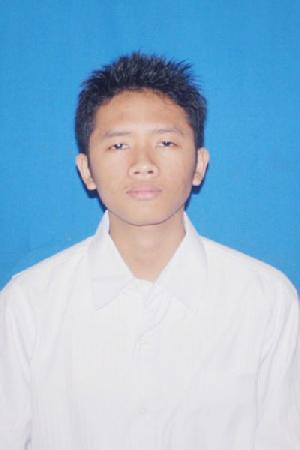
\includegraphics[height=0.3\textheight]{biodata/pas_foto.jpg}
\end{wrapfigure}

\textbf{Dewangga Winasforcepta Winardi}, lahir di Surabaya tanggal 18 Mei 1995. Penulis merupakan anak kedua dari 4 bersaudara. Penulis telah menempuh pendidikan formal TK Aisyiyah Bustanul Athfal Denpasar, SD Negeri 5 Ubung (2001-2007), SMP Negeri 5 Denpasar (2007-2010) dan SMA Negeri 4 Denpasar (2010-2013). Penulis melanjutkan studi kuliah program sarjana di Jurusan Teknik Informatika ITS. 

Selama kuliah di Teknik Informatika ITS, penulis mengambil bidang minat Algoritma Pemrograman (AP). Penulis pernah menjadi asisten dosen dan praktikum untuk mata kuliah Dasar Pemrograman (2015 dan 2016), Struktur data (2015 dan 2016). Selama menempuh perkuliahan penulis juga aktif mengikut kompetisi pemrograman tingkat nasional dan menjadi Juara 2 kategori pemrograman pada lomba COMPFEST Universitas Indonesia 2014. Selain itu penulis juga aktif di kegiatan organisasi dan kepanitiaan diantaranya menjadi staff Departemen Riset dan Teknologi HMTC ITS, wakil ketua National Programming Contest Schematics 2014, ketua National Programming Contest 2014, panitia Pemusatan Latihan Nasional 2 TOKI 2014, 2015, 2016 dan 2017 di ITS dan technical comitee Olimpiade Sains Nasional 2015 di Jogjakarta. Penulis dapat dihubungi melalui surel di \\ \texttt{dewangga.winardi@gmail.com}.

\end{document}
